%%Correcciones menores Gabriel:

%Figura 3.12 ---->> Sacar H2O adsorbida cambiar x Vapor de H2O
%Figura 4.1  ---->> Confusa..... destacar mejor con alguna figura inset u otra cosa
%Figura 3.12 ---->> Cambiar pulverizado x denso (óxido de silicio denso)
%Citar lo de la doble distribuciones con figura incluida


%%%%%%%%%%%%%%%%%%%%%%%%%%%%%%%%%%%%%%%%%%%%%%%%%
% 											                       	%
%   TESIS PARA DOCTORADO DE GUSTAVO GIMENEZ     %
%                                               %
%%%%%%%%%%%%%%%%%%%%%%%%%%%%%%%%%%%%%%%%%%%%%%%%%

%Compila Versión Final
\documentclass[a4paper,10pt,twoside,openright,titlepage]{book}

%Compila como borrador
%\documentclass[draft,a4paper,10pt,twoside,openright,titlepage]{book}

%Muestra marco para ver encabezados, cuerpo del texto, etc.
%\usepackage{showframe}

%Configuraciones
%----------------------------------------------------------------------------------------------
  %Acá van los paquetes y las definiciones de colores, renombrar comandos, nuevo comandos, etc.
  %Sección de Plugins
%--------------------------------------------------------------------------
   %Idioma, fuentes y entrada de teclado
   \usepackage[spanish,activeacute,es-tabla,es-lcroman]{babel}
   \usepackage[utf8]{inputenc}
   \usepackage{lmodern}

   %Suprime el Warning de multiples PDF por pagina
   \pdfsuppresswarningpagegroup=1
   
   %Paquete para adaptar la Bibliografia al Español
   \usepackage[datename]{babelbib}

   %Para manejar la forma en que se presentan las citas
   \usepackage[superscript]{cite}
       
   % Paquete para gestionar imágenes jpg
   \usepackage{graphicx}

   % Paquete para hacer cuadros
   \usepackage{boxedminipage} 

   %Paquete para colocar imagenes en el medio del texto
   \usepackage{wrapfig}

   %paquete para lenguaje matematico y símbolos
   \usepackage{amsmath,amssymb,amsfonts,latexsym,cancel,esint}

   % Paquete para poner colores
   \usepackage[usenames,dvipsnames]{color}

   %Para la justificación, formato y texto de los caption de las figuritas y tablas
   \usepackage{caption}

   %Paquete para poder poner imagenes una al lado de la otra
   \usepackage{subcaption}
   
   %Para hacer graficos cons tikz, con gnuplot y poder exportarlos como pdf
       \usepackage{tikz}
       \usepackage{tikzpagenodes}
     
           %Librerias Tikz Extra
             \usetikzlibrary{shapes,arrows}
             \usetikzlibrary{shapes.arrows, fadings}
             \usetikzlibrary{shadows.blur}
             \usetikzlibrary{shapes.symbols}
             \usetikzlibrary{decorations.pathreplacing}
             \usetikzlibrary{fit}
             \usetikzlibrary{calc}
             \usetikzlibrary{positioning}
             \usetikzlibrary{matrix}

   %Para hacer lineas gruesa y tablas lindas
   \usepackage{booktabs}

   %Para Formatear los capitulos
   \usepackage{titlesec}

   %Herramientas para parches
   %Yo lo use para Cambiar el nombre de la Bibliografia
   \usepackage{etoolbox}
   
   %Para Tablas multicolumnas, multifilas
   \usepackage{multirow,multicol,array} 

   %Para rota Texto
   \usepackage{rotating} 

   %Para los Indices parciales en las portadas de los capitulos
   \usepackage[nohints]{minitoc}

   %Paquete para personalizar encabezados y notas al pie
   \usepackage{fancyhdr}   

   %Para que no numere las paginas en blanco (borrar los header y footnotes)
   \usepackage{emptypage}

   %Para carga Atributos, Propiedades y Titulos al PDF
   \usepackage[hidelinks,colorlinks]{hyperref}

   %Para la lista de abreviaturas
   \usepackage[acronym,nonumberlist,nomain]{glossaries}
   \makeglossaries
   
   %Para hacer un indice alfabetico
   \usepackage{imakeidx}
   \makeindex[columns=2, options= -s Tesis.ist]
   \indexsetup{othercode=\footnotesize}
   %Muestra el indexado en el costado
   %\usepackage{showidx}
   
   %Para Imprimir el LayOut del documento
   \usepackage{layout}

   %Para hacer quimica
   \usepackage{chemfig}

   %para meter text de relleno
   \usepackage{blindtext}

   %Paquete gestor de unidades
   \usepackage[version-1-compatibility]{siunitx}
   \sisetup{output-decimal-marker = {,}}

   %Para Colocar objetos en el fondo, en mi caso los indicadores laterales
   \usepackage[contents={},opacity=1,scale=1,color=black]{background}
   %--------------------------------------------------------------------------

%SUprimir log de Overfull y UNdelfull
%--------------------------------------------------------------------------
    \newcommand{\NoBadBoxesLog}{
      \hfuzz=\maxdimen \vfuzz=\maxdimen 
      \newdimen\hfuzz  \let\vfuzz=\hfuzz
      \hbadness=10000    \vbadness=10000 
      \newcount\hbadness \let\vbadness=\hbadness 
      }

%Propiedades del Documento
%--------------------------------------------------------------------------
   \hypersetup{
   pdftitle={Tesis Gustavo Giménez},
   pdfauthor={Gustavo Giménez},
   pdfsubject={Tesis Doctoral}, %subject of the document
   pdfcreator={Tex},
   pdfproducer={PDFLatex},
   pdfkeywords={UBA,nanomateriales,MEMS,NEMS,INTI},
   % %pdftoolbar=false, % toolbar hidden
   pdfmenubar=true, %menubar shown
   pdfhighlight=/O, %effect of clicking on a link
   % pdfpagemode=UseOutlines,%UseNone, %aucun mode de page
   % pdfpagelayout=TwoPageRight,%SinglePage, %ouverture en simple page
   % pdffitwindow=true, %pages ouvertes entierement dans toute la fenetre
   % bookmarksopenlevel=2,
   %    colorlinks=false,       % false: boxed links; true: colored links
   linkcolor=black,          % color of internal links (change box color with linkbordercolor)
   citecolor=grisoscuro,        % color of links to bibliography
   urlcolor=grisoscuro,          % color of external link
   %backref=true
   }
   %--------------------------------------------------------------------------

  %Aca Pongo los archivos de Formato Personalizados:
  %Margenes, tamaños, titulos, lineas, capitulos, caption, etc.
  %%%%%%%%%%%%%%%%%%%%%%%%%%%%%%%%%%%%%%%%%%%%%%%%%%%%%%%%%%%%%%%%%%%
%   Aca van los Formatos Personalizados de todo el documento	  %
%%%%%%%%%%%%%%%%%%%%%%%%%%%%%%%%%%%%%%%%%%%%%%%%%%%%%%%%%%%%%%%%%%%

%Formato General del Documento
%------------------------------------------------------------
 
 %Intercambio los margenes derechos e izquierdos
 %------------------------------------------------------------
 \let\tmp\oddsidemargin
 \let\oddsidemargin\evensidemargin
 \let\evensidemargin\tmp
 \reversemarginpar

 %La class book por default pone un espacio para notas marginales en el lado derecho para las paginas 
 %impares y en el izquierdo para las pares, yo lo invertí para que me quede mas amplio el espacio para 
 %la unión de las paginas en el lomo del libro, la costura.
 

    % Defino los margenes bien personalizados.
    % Zona de la pagina ocupada por el texto
    % Información detallada: http://en.wikibooks.org/wiki/LaTeX/Page_Layout
    % O descomentar la linea  \layout 
	% \layout
 	%------------------------------------------------------------------------------------------------------------------ 
 		% 	    \hoffset = 2 cm                          % OffSet desde el borde izquierdo de la pagina
 		% 		\voffset = 2 cm                          % OffSet desde el borde Superior de la pagina
 		% 		\topmargin = -2.54 cm                    % Desde el borde superior de la pagina hasta el texto + 1 inch
		% 		\oddsidemargin = -2.54 cm                % Desde el borde izquierdo de la pagina hasta el texto + 1 inc
		% 		\headsep =  0 cm                         % Separación entre el encabezado y el texto	
 		% 		\textwidth = 17 cm                       % Ancho del texto y define margen derecho - margen - offset
 		% 		\textheight = 23.5 cm                    % Largo del texto y margen inferior - margen - offset
 		% 		\headheight = 0.1 cm                     % Espacio del cuadro de texto del Encabezado
		% 		\footskip = 1.5 cm                       %Espacio para el pie de pagina 
 		%    	\marginparwidth = 95pt					 %Ancho de las notas al margen
 		% 	    \marginparsep = 25pt					 %Separación margen-texto
 	%------------------------------------------------------------------------------------------------------------------

%Formato de las Cabeceras, los Pie de Pagina y la numeracion
%------------------------------------------------------------
	%Cambio el Header para que no salga la palabra "Capitulo"
	\addto{\captionsspanish}{\def\chaptername{}}

	%Cambio el Color de la Headrule
	\let\headruleORIG\headrule
	\renewcommand{\headrule}{\color{grisoscuro}\headruleORIG}
	
	%Estilo de las Cabeceras y Pie de pagina para los precapitulos
	\fancypagestyle{frontmatter}{
		\fancyhead{}   							%Borro Cabeceras
		\renewcommand{\headrulewidth}{0pt} 		%Borro Headrule							
		\fancyfoot[C]{\thepage}    				%Numero de pagina centrado
		}
	
	%Estilo de las Cabeceras y Pie de pagina para el cuerpo principal
	\fancypagestyle{mainmatter}{
		\fancyfoot{}													   % Borro las paginas al pie
		\renewcommand{\headrulewidth}{1pt}  							   % Borro la Linea del encabecera		
		\fancyfoot[LE,RO]{\color{grisoscuro}\bfseries\thepage}             % Pongo el numero de pagina en todas la paginas en el lado exterior
	 	\fancyhead[LE]{\color{grisoscuro}\bfseries\nouppercase{\leftmark}} % Pongo el capitulo arriba a la derecha en las paginas pares 
	    \fancyhead[RO]{\color{grisoscuro}\bfseries\nouppercase{\rightmark}}% Pongo la sección arriba a la izquierda en las impares
	    }
	
	%Estilo de las Cabeceras y Pie de pagina para los postcapitulos
	\fancypagestyle{backmatter}{
		\fancyhead{}
		\fancyfoot{}										    %Borro Cabeceras
		\renewcommand{\headrulewidth}{0pt} 				        %Borro Headrule							
		\fancyfoot[LE,RO]{\color{grisoscuro}\bfseries\thepage}  % Pongo el numero de pagina en todas la paginas en el lado exterior
		}
 %--------------------------------------------------------------

%Formato de las Etiquetas (Referencias, Capitulos, etc)
%------------------------------------------------------------
 %Cambiar el nombre de Bibliografia por Referencias
 \patchcmd{\thebibliography}{\chapter*{\bibname}}{\chapter*{Referencias}}{}{}
 %-------------------------------------------------------------

%Formato de los Titulos de los capitulos
%------------------------------------------------------------
    %Ubicación Espacial del conjunto "Titulo" de Capitulos
      \titlespacing*{\chapter}  %Seccion a modificar
 			 {-3cm}             %Indentación Izquierda
 			 {-1cm}            %Espacio Anterior
 			 {50pt} 	        %Espacio Posterior
 			 [0cm]	           %Indentación Derecha
    
    %Formato para Todos los Capitulos, solo lo uso para el Indice General
	 \titleformat{\chapter}[display]
			{\Huge\filleft\scshape\color{grisoscuro}}      	 %Formato para etiqueta y texto
	 		{}	
	 		{20pt}  	     %Separación Etiqueta/Texto                
	 		{}               %Codigo anterior
	 		[]   %Codigo Posteior  \titlerule\vspace{2ex}\filright\vspace{2ex}]
	
	%Variables para ubicar el numero de capitulo	
	 \newlength\NumCapX
	 \setlength\NumCapX{-1cm}  %Aumentar es mas para arriba
	 \newlength\NumCapY	
	 \setlength\NumCapY{-2cm}  %Aumentar es mas para el exterior		

	%Formato para el titulo de los Indices
	 \newcommand{\FormatoIndice}{
	 		\titleformat{name=\chapter,numberless}[display]						 %Sin Numerar
			{\Huge\filleft\scshape\color{grisoscuro}}      	 %Formato para etiqueta y texto
	 		{\begin{tikzpicture}[remember picture,overlay] 						 %Cuadrado con el numero
				\node[at={($(\NumCapX,\NumCapY)$)},anchor=center,font=\rmfamily\fontsize{300pt}{0pt}\bf\selectfont\color{grisoscuro},opacity=0.2] (texto) {\textit{I}};
				\node at (-12.16,-2) {\rule{25cm}{0.5mm}};
				\end{tikzpicture}
			}		
	 		{20pt}  	    				 %Separación Etiqueta/Texto                
	 		{\vspace*{-0.15cm}}              %Codigo anterior
	 		[]   				 %Codigo Posteior
	 } 

	%Formato Para los Capitulos Numerados y que el título ocupa una sola linea
 	 \newcommand{\FormatoCapituloUnaLinea}{
 		\titleformat{\chapter}     						     %Seccion a modificar
			[display]					 			 		 %Formato separado en dos renglones separados
			{\Huge\filleft\scshape\color{grisoscuro}}      	 %Cuadrado con el numero
			{\begin{tikzpicture}[remember picture,overlay]
				\node[at={($(\NumCapX,\NumCapY)$)},anchor=center,font=\rmfamily\fontsize{300pt}{0pt}\bf\selectfont\color{grisoscuro},opacity=0.2] (texto) {\textit{\thechapter}};
				\node at (-12.16,-2) {\rule{25cm}{0.5mm}};
			    \end{tikzpicture}
			}
	 		{20pt}  	     %Separación Etiqueta/Texto                
	 		{}               %Codigo anterior
	 		[]   %Codigo Posteior 
	 		}	
 	 		
	%Formato Para los Capitulos Numerados y que el título ocupa dos lineas
 	 \newcommand{\FormatoCapituloDosLineas}{
 		\titleformat{\chapter}     						     %Seccion a modificar
			[display]					 			 		 %Formato separado en dos renglones separados
			{\Huge\filleft\scshape\color{grisoscuro}}      	 %Cuadrado con el numero
			{\begin{tikzpicture}[remember picture,overlay]
				\node[at={($(\NumCapX,\NumCapY)$)},anchor=center,font=\rmfamily\fontsize{300pt}{0pt}\bf\selectfont\color{grisoscuro},opacity=0.2] (texto) {\textit{\thechapter}};
				\node at (-12.16,-2) {\rule{25cm}{0.5mm}};
				\end{tikzpicture}
			}
	 		{20pt}  	     		 %Separación Etiqueta/Texto                
	 		{\vspace*{-1.05cm}}      %Codigo anterior
	 		[]  		 %Codigo Posteior  
	 		}	
	
	%Formato para el titulo de los Anexos
	 \newcommand{\FormatoAnexoA}{
	 		\titleformat{name=\chapter,numberless}[display]						 %Sin Numerar
			{\Huge\filleft\scshape\color{grisoscuro}}      	 %Formato para etiqueta y texto
	 		{\begin{tikzpicture}[remember picture,overlay] 						 %Cuadrado con el numero
				\node[at={($(\NumCapX,\NumCapY)$)},anchor=center,font=\rmfamily\fontsize{300pt}{0pt}\bf\selectfont\color{grisoscuro},opacity=0.2] (texto) {\textit{A}};
				\node at (-12.16,-2) {\rule{25cm}{0.5mm}};
				\end{tikzpicture}
			}		
	 		{20pt}  	    				 %Separación Etiqueta/Texto                
	 		{\vspace*{-1.05cm}}              %Codigo anterior
	 		[]   				 %Codigo Posteior
	 }
	 \newcommand{\FormatoAnexoB}{
	 		\titleformat{name=\chapter,numberless}[display]						 %Sin Numerar
			{\Huge\filleft\scshape\color{grisoscuro}}      	 %Formato para etiqueta y texto
	 		{\begin{tikzpicture}[remember picture,overlay] 						 %Cuadrado con el numero
				\node[at={($(\NumCapX,\NumCapY)$)},anchor=center,font=\rmfamily\fontsize{300pt}{0pt}\bf\selectfont\color{grisoscuro},opacity=0.2] (texto) {\textit{B}};
				\node at (-12.16,-2) {\rule{25cm}{0.5mm}};
				\end{tikzpicture}
			}		
	 		{20pt}  	    				 %Separación Etiqueta/Texto                
	 		{\vspace*{-0.15cm}}              %Codigo anterior
	 		[]   				 %Codigo Posteior
	 }

	  \newcommand{\FormatoAnexoC}{
	 		\titleformat{name=\chapter,numberless}[display]						 %Sin Numerar
			{\Huge\filleft\scshape\color{grisoscuro}}      	 %Formato para etiqueta y texto
	 		{\begin{tikzpicture}[remember picture,overlay] 						 %Cuadrado con el numero
				\node[at={($(\NumCapX,\NumCapY)$)},anchor=center,font=\rmfamily\fontsize{300pt}{0pt}\bf\selectfont\color{grisoscuro},opacity=0.2] (texto) {\textit{C}};
				\node at (-12.16,-2) {\rule{25cm}{0.5mm}};
				\end{tikzpicture}
			}		
	 		{20pt}  	    				 %Separación Etiqueta/Texto                
	 		{\vspace*{-0.15cm}}              %Codigo anterior
	 		[]   				 %Codigo Posteior
	 }

	%Formato para el titulo del Capitulo Referencias
	  \newcommand{\FormatoReferencias}{
	  		\titleformat{name=\chapter,numberless}[display]  %Sin Numerar
		 	{\Huge\filleft\scshape\color{grisoscuro}}      	 %Formato para etiqueta y texto
	  	 	{\begin{tikzpicture}[remember picture,overlay]   %Cuadrado con el numero
		 		\node[at={($(\NumCapX,\NumCapY)$)},anchor=center,font=\rmfamily\fontsize{300pt}{0pt}\bf\selectfont\color{grisoscuro},opacity=0.2] (texto) {\textit{R}};
		 		\node at (-12.16,-2) {\rule{25cm}{0.5mm}};
		 		\end{tikzpicture}
		 	}
	  		{20pt}  	     %Separación Etiqueta/Texto                
	  		{}               %Codigo anterior
	  		[]   %Codigo Posteior  
	  }

	%-------------------------------------------------------------

%Indicador lateral de capitulos
%------------------------------------------------------------
	
	%Definiciones Generales de variables para los loops if
	 \newif\ifMaterialInd
	 \newif\ifMaterialCap
	 \newif\ifMaterialAxUno
	 \newif\ifMaterialAxDos
	 \newif\ifMaterialAxTres
	 \newif\ifMaterialBib
	 \newif\ifMaterialAlf

	%Posiciones Iniciales de los indicadores laterales
	 \newlength\PosVertical
	 \setlength\PosVertical{6.56cm}       %Aumentar es mas para arriba
	 \newlength\PosHorizontal	
	 \setlength\PosHorizontal{10.2cm}  %Aumentar es mas para el exterior

	%Con \AddLabelsInd se agregan los indicadores laterales de los indices
	 \newcommand\AddLabelsInd{
	 \MaterialIndtrue
	 \AddEverypageHook{
	 	\ifMaterialInd
	 		\ifodd\value{page} 
  				\backgroundsetup{
	 				  angle=90, %Ojo!! Invierte las coordenadas!!
	 				  contents={
	 				  \begin{tikzpicture}[remember picture,overlay] 
	 				    \node[at={($(\PosVertical,-\PosHorizontal)$)}] % Las coordenadas son (y,-x)
	 					(cuadrado) {\tikz {\draw[draw=none,fill=grisoscuro] (0,0) rectangle ++(3,1);} };
	 					\node[at={($(cuadrado.center)+(0,0.2)$)},anchor=center,font=\large\filleft\scshape,text=white](texto) {Índice};
	 					\end{tikzpicture}
	 				  }
	 				 }
  			\else
	 				 \backgroundsetup{
	 				  angle=90, %Ojo!! Invierte las coordenadas!!
	 				  contents={
	 				    \begin{tikzpicture}[remember picture,overlay] 
	 				    \node[at={($(\PosVertical,\PosHorizontal)$)}] % Las coordenadas son (y,-x)
	 					(cuadrado) {\tikz {\draw[draw=none,fill=grisoscuro] (0,0) rectangle ++(3,1);} };
	 					\node[at={($(cuadrado.center)+(0,-0.1)$)},anchor=center,font=\large\filleft\scshape,text=white](texto) {Índice};
	 					\end{tikzpicture}
	 				  }
	 				 }
  			\fi
	 	\BgMaterial
	 	\else\relax\fi}
	 	}	 

	%Con \AddLabelsCap se agregan los indicadores laterales de los capitulos
	 \newcommand\AddLabelsCap{
	 \MaterialCaptrue
	 \AddEverypageHook{
	 	\ifMaterialCap
	 		\ifodd\value{page} 
  				\backgroundsetup{
	 				  angle=90, %Ojo!! Invierte las coordenadas!!
	 				  contents={
	 				  \begin{tikzpicture}[remember picture,overlay] 
	 				    \node[at={($(\PosVertical,-\PosHorizontal)-(\thechapter,0)$)}] % Las coordenadas son (y,-x)
	 					(cuadrado) {\tikz {\draw[draw=none,fill=grisoscuro] (0,0) rectangle ++(3,1);} };
	 					\node[at={($(cuadrado.center)+(0,0.2)$)},anchor=center,font=\large\filleft\scshape,text=white](texto) {Capítulo \thechapter};
	 					\end{tikzpicture}
	 				  }
	 				 }
  			\else
	 				 \backgroundsetup{
	 				  angle=90, %Ojo!! Invierte las coordenadas!!
	 				  contents={
	 				    \begin{tikzpicture}[remember picture,overlay] 
	 				    \node[at={{($(\PosVertical,\PosHorizontal)-(\thechapter,0)$)}}] % Las coordenadas son (y,-x)
	 					(cuadrado) {\tikz {\draw[draw=none,fill=grisoscuro] (0,0) rectangle ++(3,1);} };
	 					\node[at={($(cuadrado.center)+(0,-0.1)$)},anchor=center,font=\large\filleft\scshape,text=white](texto) {Capítulo \thechapter};
	 					\end{tikzpicture}
	 				  }
	 				 }
  			\fi
	 	\BgMaterial
	 	\else\relax\fi}
	 	}

	%Con \AddLabelsAxUno se agregan los indicaroes laterales Anexo A
     \newcommand\AddLabelsAxUno{
	 \MaterialAxUnotrue
	 \AddEverypageHook{
	 	\ifMaterialAxUno
	 		\ifodd\value{page}
  				\backgroundsetup{
	 				  angle=90, %Ojo!! Invierte las coordenadas!!
	 				  contents={
	 				  \begin{tikzpicture}[remember picture,overlay] 
	 					\node[at={($(\PosVertical,-\PosHorizontal)-(\thechapter+1,0)$)}] % Las coordenadas son (y,-x)
	 					(cuadrado) {\tikz {\draw[draw=none,fill=grisoscuro] (0,0) rectangle ++(3,1);} };
	 					\node[at={($(cuadrado.center)+(0,0.2)$)},anchor=center,font=\large\filleft\scshape,text=white](texto) {Anexo A};
	 					\end{tikzpicture}
	 				  }
	 				 }
  			\else
	 				 \backgroundsetup{
	 				  angle=90, %Ojo!! Invierte las coordenadas!!
	 				  contents={
	 				    \begin{tikzpicture}[remember picture,overlay] 
	 				    \node[at={($(\PosVertical,\PosHorizontal)-(\thechapter+1,0)$)}]  % Las coordenadas son (y,-x)
	 				    (cuadrado) {\tikz {\draw[draw=none,fill=grisoscuro] (0,0) rectangle ++(3,1);} };
	 				    \node[at={($(cuadrado.center)+(0,-0.1)$)},anchor=center,font=\large\filleft\scshape,text=white] (texto) {Anexo A};
	 					\end{tikzpicture}
	 				  }
	 				 }
  			\fi
	 	\BgMaterial
	 	\else\relax\fi}
	 	}

	%Con \AddLabelsAxDos se agregan los indicaroes laterales Anexo B
	 \newcommand\AddLabelsAxDos{
	 \MaterialAxDostrue
	 \AddEverypageHook{
	 	\ifMaterialAxDos
	 		\ifodd\value{page}
  				\backgroundsetup{
	 				  angle=90, %Ojo!! Invierte las coordenadas!!
	 				  contents={
	 				  \begin{tikzpicture}[remember picture,overlay] 
	 					\node[at={($(\PosVertical,-\PosHorizontal)-(\thechapter+2,0)$)}] % Las coordenadas son (y,-x)
	 					(cuadrado) {\tikz {\draw[draw=none,fill=grisoscuro] (0,0) rectangle ++(3,1);} };
	 					\node[at={($(cuadrado.center)+(0,0.2)$)},anchor=center,font=\large\filleft\scshape,text=white](texto) {Anexo B};
	 					\end{tikzpicture}
	 				  }
	 				 }
  			\else
	 				 \backgroundsetup{
	 				  angle=90, %Ojo!! Invierte las coordenadas!!
	 				  contents={
	 				    \begin{tikzpicture}[remember picture,overlay] 
	 				    \node[at={($(\PosVertical,\PosHorizontal)-(\thechapter+2,0)$)}]  % Las coordenadas son (y,-x)
	 				    (cuadrado) {\tikz {\draw[draw=none,fill=grisoscuro] (0,0) rectangle ++(3,1);} };
	 				    \node[at={($(cuadrado.center)+(0,-0.1)$)},anchor=center,font=\large\filleft\scshape,text=white] (texto) {Anexo B};
	 					\end{tikzpicture}
	 				  }
	 				 }
  			\fi
	 	\BgMaterial
	 	\else\relax\fi}
	 	}
	
	%Con \AddLabelsAxDos se agregan los indicaroes laterales Anexo C
	 \newcommand\AddLabelsAxTres{
	 \MaterialAxTrestrue
	 \AddEverypageHook{
	 	\ifMaterialAxTres
	 		\ifodd\value{page}
  				\backgroundsetup{
	 				  angle=90, %Ojo!! Invierte las coordenadas!!
	 				  contents={
	 				  \begin{tikzpicture}[remember picture,overlay] 
	 					\node[at={($(\PosVertical,-\PosHorizontal)-(\thechapter+3,0)$)}] % Las coordenadas son (y,-x)
	 					(cuadrado) {\tikz {\draw[draw=none,fill=grisoscuro] (0,0) rectangle ++(3,1);} };
	 					\node[at={($(cuadrado.center)+(0,0.2)$)},anchor=center,font=\large\filleft\scshape,text=white](texto) {Anexo C};
	 					\end{tikzpicture}
	 				  }
	 				 }
  			\else
	 				 \backgroundsetup{
	 				  angle=90, %Ojo!! Invierte las coordenadas!!
	 				  contents={
	 				    \begin{tikzpicture}[remember picture,overlay] 
	 				    \node[at={($(\PosVertical,\PosHorizontal)-(\thechapter+3,0)$)}]  % Las coordenadas son (y,-x)
	 				    (cuadrado) {\tikz {\draw[draw=none,fill=grisoscuro] (0,0) rectangle ++(3,1);} };
	 				    \node[at={($(cuadrado.center)+(0,-0.1)$)},anchor=center,font=\large\filleft\scshape,text=white] (texto) {Anexo C};
	 					\end{tikzpicture}
	 				  }
	 				 }
  			\fi
	 	\BgMaterial
	 	\else\relax\fi}
	 	}
	 	
	%Con \AddLabelsBib se agregan los indicaroes laterales para la bibliografia
	 \newcommand\AddLabelsBib{
	 \MaterialBibtrue
	 \AddEverypageHook{
	 	\ifMaterialBib
	 		\ifodd\value{page}
  				\backgroundsetup{
	 				  angle=90, %Ojo!! Invierte las coordenadas!!
	 				  contents={
	 				  \begin{tikzpicture}[remember picture,overlay] 
	 					\node[at={($(\PosVertical,-\PosHorizontal)-(\thechapter+4,0)$)}] % Las coordenadas son (y,-x)
	 					(cuadrado) {\tikz {\draw[draw=none,fill=grisoscuro] (0,0) rectangle ++(3,1);} };
	 					\node[at={($(cuadrado.center)+(0,0.2)$)},anchor=center,font=\large\filleft\scshape,text=white](texto) {Referencias};
	 					\end{tikzpicture}
	 				  }
	 				 }
  			\else
	 				 \backgroundsetup{
	 				  angle=90, %Ojo!! Invierte las coordenadas!!
	 				  contents={
	 				    \begin{tikzpicture}[remember picture,overlay] 
	 				    \node[at={($(\PosVertical,\PosHorizontal)-(\thechapter+4,0)$)}]  % Las coordenadas son (y,-x)
	 				    (cuadrado) {\tikz {\draw[draw=none,fill=grisoscuro] (0,0) rectangle ++(3,1);} };
	 				    \node[at={($(cuadrado.center)+(0,-0.1)$)},anchor=center,font=\large\filleft\scshape,text=white] (texto) {Referencias};
	 					\end{tikzpicture}
	 				  }
	 				 }
  			\fi
	 	\BgMaterial
	 	\else\relax\fi}
	 	}

	%Con \AddLabelsAlf se agregan los indicadores laterales del indice alfabetico
	 \newcommand\AddLabelsAlf{
	 \MaterialAlftrue
	 \AddEverypageHook{
	 	\ifMaterialAlf
	 		\ifodd\value{page} 
  				\backgroundsetup{
	 				  angle=90, %Ojo!! Invierte las coordenadas!!
	 				  contents={
	 				  \begin{tikzpicture}[remember picture,overlay] 
	 				    \node[at={($(\PosVertical,-\PosHorizontal)-(\thechapter+6,0)$)}] % Las coordenadas son (y,-x)
	 					(cuadrado) {\tikz {\draw[draw=none,fill=grisoscuro] (0,0) rectangle ++(4,1);} };
	 					\node[at={($(cuadrado.center)+(0,0.2)$)},anchor=center,font=\large\filleft\scshape,text=white](texto) {Índice Alfabético};
	 					\end{tikzpicture}
	 				  }
	 				 }
  			\else
	 				 \backgroundsetup{
	 				  angle=90, %Ojo!! Invierte las coordenadas!!
	 				  contents={
	 				    \begin{tikzpicture}[remember picture,overlay] 
	 				    \node[at={($(\PosVertical,\PosHorizontal)-(\thechapter+6,0)$)}] % Las coordenadas son (y,-x)
	 					(cuadrado) {\tikz {\draw[draw=none,fill=grisoscuro] (0,0) rectangle ++(4,1);} };
	 					\node[at={($(cuadrado.center)+(0,-0.1)$)},anchor=center,font=\large\filleft\scshape,text=white](texto) {Índice Alfabético};
	 					\end{tikzpicture}
	 				  }
	 				 }
  			\fi
	 	\BgMaterial
	 	\else\relax\fi}
	 	}	 	
	
	%Con estos comandos se borran los indicadores laterales	
	 \newcommand\RemoveLabelsInd{\MaterialIndfalse}
	 \newcommand\RemoveLabelsCap{\MaterialCapfalse}
	 \newcommand\RemoveLabelsAxUno{\MaterialAxUnofalse}
	 \newcommand\RemoveLabelsAxDos{\MaterialAxDosfalse}
	 \newcommand\RemoveLabelsAxTres{\MaterialAxTresfalse}
	 \newcommand\RemoveLabelsBib{\MaterialBibfalse}
	 \newcommand\RemoveLabelsAlf{\MaterialAlffalse}

%Formato de los mini-indices de los capitulos 
%------------------------------------------------------------
  \mtcindent=0pt  %indentacion de los Indices de los capitulos
  \def\mtctitle{Contenido}  %Cambio el Nombre del indice de los capitulos

  \setcounter{tocdepth}{3}
  \setcounter{minitocdepth}{3} 
  \setcounter{secnumdepth}{3}
  \renewcommand{\thesubsubsection}{\thesubsection.\roman{subsubsection}}
 %-------------------------------------------------------------

%Formato de la Bibliografia
%------------------------------------------------------------
 %links externos con misma fuente que el texto
 \urlstyle{same}

%Formato de la lista de siglas, abreviaturas y nomenclaturas
%------------------------------------------------------------
 	\newlength\myitemwidth

 	%Declara el formato de la lista de items
	\setlength\myitemwidth{3cm}
	\newlist{listasiglas}{description}{1}
	\setlist[listasiglas]{
  		labelindent = 0pt ,
  		labelsep    = 0pt ,
 		leftmargin  = \myitemwidth ,
 		labelwidth  = \myitemwidth ,
 		itemindent  = 0pt ,
 		format      = \bfseries ,
 		parsep      = -2pt
		}

	%Ledigo al paquete de acronimos que use la lista formateada	
	\DeclareAcroListStyle{estilosiglas}{list}{list = listasiglas}
  	\acsetup{ list-style = estilosiglas,only-used=false }	

%Formato de del indice alfabetico
%------------------------------------------------------------
	
	%Dos Columnas y tamaño mas pequeño
	\makeindex[columns=2, options= -s Tesis.ist]
	\indexsetup{othercode=\footnotesize}

%Formato de las notas al margen
%------------------------------------------------------------
 \let\oldmarginpar\marginpar
 \renewcommand{\marginpar}[1]{\oldmarginpar{\itshape{\textcolor{red}{#1}}}}
 %-----------------------------------------------------------
 
%Colores Personalizados
%------------------------------------------------------------
  \definecolor{grisoscuro}{gray}{0.3}          %El gris oscuro de los Capitulos
  \definecolor{marron}{rgb}{0.647,0.165,0.165} %Los use en los graficos de VC del Au INTI contra Au CNEA
  \definecolor{rojo}{rgb}{1,0,0} 			   %Los use en los graficos de VC del Au INTI contra Au CNEA	
  \definecolor{oliva}{rgb}{0.627,0.502,0.125}  %Los use en los graficos de VC del Au INTI contra Au CNEA
 %------------------------------------------------------------

%Formato de los caption para las tablas y figuras y ecuaciones
%------------------------------------------------------------
 \captionsetup[table]{singlelinecheck=false,justification=justified ,labelfont=bf,font=small,position=top,skip=0pt}
 \captionsetup[subtable]{labelfont=bf,font=small,position=top,aboveskip=10pt,belowskip=10pt,labelsep=period,labelformat=empty}
 \captionsetup[figure]{singlelinecheck=false,justification=justified,labelfont=bf,font=footnotesize,position=bottom,aboveskip=10pt,belowskip=-10pt}
 \captionsetup[subfigure]{singlelinecheck=false,justification=justified,labelfont=bf,font=scriptsize,position=top,aboveskip=0pt,belowskip=10pt,labelsep=period,labelformat = simple,width=.95\textwidth}

%Formato de las viñetas
%------------------------------------------------------------
	\renewcommand{\labelitemi}{$\bullet$}
 %-----------------------------------------------------------

%Abreviaturas para cosas que voy a usar mucho
%------------------------------------------------------------
   
   %Sondas electroquimcias
   \newcommand{\hq}{HQ\index{hidroquinona}}
   \newcommand{\fe}{FeCN\index{ferrocianuro de potasio}\index{ferricianuro de potasio}}
   \newcommand{\ru}{ARu\index{aminorutenio}}
   \newcommand{\fc}{FcOH\index{ferroceno metanol}}  

   %Formula Aminorutenio desarrollada
   \newcommand{\aminorutenio}{[Ru(NH$_3$)$_6]^{3+}$\index{aminorutenio}}
   \newcommand{\aminorutenioCompleto}{Ru(NH$_3$)$_6$Cl{$_3$}\index{aminorutenio}}

   %Formula desarrollada para la cupla Ferro/Ferri
   \newcommand{\ferroferri}{[Fe(CN)$_6]^{4-}$\textsuperscript{/}$^{3-}$\index{ferrocianuro de potasio}\index{ferricianuro de potasio}}
   \newcommand{\ferro}{[Fe(CN)$_6]^{4-}$\index{ferrocianuro de potasio}}
   \newcommand{\ferri}{[Fe(CN)$_6]^{3-}$\index{ferricianuro de potasio}}
   \newcommand{\Ferro}{K$_4$Fe(CN)$_6$\index{ferrocianuro de potasio}}
   \newcommand{\Ferri}{K$_3$Fe(CN)$_6$\index{ferricianuro de potasio}}
   \newcommand{\ferroCompleto}{K$_4$Fe(CN)$_6$.3H$_2$O\index{ferrocianuro de potasio}}
   \newcommand{\ferriCompleto}{K$_3$Fe(CN)$_6$.3H$_2$O\index{ferricianuro de potasio}}
  
   %Formula desarrollada para la Ferroceno
   \newcommand{\ferroceno}{C$_{11}$H$_{12}$OFe\index{ferroceno metanol}}

   %Formula desarrollada para el Hidroquinona
   \newcommand{\hidroquinona}{C$_6$H$_4$O$_2$\index{hidroquinona}}

   %Peliculas Delgadas Mesoporosas de oxido de SIlicio
   \newcommand{\pdm}{PDM\index{película!mesoporosa}}
   \newcommand{\pdmF}{SF\index{película!mesoporosa Si(F127)}}
   \newcommand{\pdmC}{SC\index{película!mesoporosa Si(CTAB)}}
   \newcommand{\pdmZ}{SZF\index{película!mesoporosa Zr/Si(F127)}}
   \newcommand{\pdmZB}{SZB\index{película!mesoporosa Zr/Si(Brij58)}}


%Leyendas para los graficos
%------------------------------------------------------------
	%Para los graficos de los problemas tecnologicos Circulitos con Colores
	\newcommand{\unorojo}{\begin{tikzpicture}[baseline={([yshift=-0.8mm]current bounding box.center)}]\node[circle,fill=red!80,text=white,inner sep=1,anchor=mid] at (0,0) {\scriptsize{1}};\end{tikzpicture}\space}
	\newcommand{\dosvioleta}{\begin{tikzpicture}[baseline={([yshift=-0.8mm]current bounding box.center)}]\node[circle,fill=violet!70,text=white,inner sep=1,anchor=mid] at (0,0) {\scriptsize{2}};\end{tikzpicture}\space}
	\newcommand{\tresamarillo}{\begin{tikzpicture}[baseline={([yshift=-0.8mm]current bounding box.center)}]\node[circle,fill=yellow,text=white,inner sep=1,anchor=mid] at (0,0) {\scriptsize{3}};\end{tikzpicture}\space}
	\newcommand{\cuatronaranja}{\begin{tikzpicture}[baseline={([yshift=-0.8mm]current bounding box.center)}]\node[circle,fill=orange!80,text=white,inner sep=1,anchor=mid] at (0,0) {\scriptsize{4}};\end{tikzpicture}\space}

	%Las rayas con los colores mas comunes
   	\newbox{\negro}
  		\savebox{\negro}{\raisebox{2pt}{\tikz{\draw[black,solid,line width=0.8pt](0,0) -- (4mm,0);}}}
	\newbox{\marron} 
	  	\savebox{\marron}{\raisebox{2pt}{\tikz{\draw[marron,solid,line width=0.8pt](0,0) -- (4mm,0);}}}
	\newbox{\rojo} 
	  	\savebox{\rojo}{\raisebox{2pt}{\tikz{\draw[rojo,solid,line width=0.8pt](0,0) -- (4mm,0);}}}
	\newbox{\oliva} 
	  	\savebox{\oliva}{\raisebox{2pt}{\tikz{\draw[oliva,solid,line width=0.8pt](0,0) -- (4mm,0);}}}	
	\newbox{\azul} 
	  	\savebox{\azul}{\raisebox{2pt}{\tikz{\draw[blue,solid,line width=0.8pt](0,0) -- (4mm,0);}}}
	\newbox{\gris} 
	  	\savebox{\gris}{\raisebox{2pt}{\tikz{\draw[gray,solid,line width=0.8pt](0,0) -- (4mm,0);}}}
	\newbox{\verde} 
	  	\savebox{\verde}{\raisebox{2pt}{\tikz{\draw[OliveGreen,solid,line width=0.8pt](0,0) -- (4mm,0);}}}
	\newbox{\punteado}
		\savebox{\punteado}{\raisebox{2pt}{\tikz{\draw[black,dashed,line width=0.8pt](0,0) -- (3.2mm,0);}}}
	  	  

%Separación de las sílabas
%------------------------------------------------------------
	\hyphenation{Pasteur Kelvin PMMA Biopack sonda-electrodo hexadeciltrimetilamonio INTI telluride adherencia Fourier}
 %-----------------------------------------------------------
  %------------------------------------------------\--------------------------------------------\label{sec:microfabricacion}

% Elimina todos los UnderFull y OverFull BadBox's.
%----------------------------------------------------------------------------------------------
  %\NoBadBoxesLog
  %--------------------------------------------------------------------------------------------

\begin{document}

%Incluyo la Portada
%----------------------------------------------------------------------------------------------
  \begin{titlepage}

%Portada

		%Universidad
		\begin{center}
		\sc{\LARGE{Universidad de Buenos Aires\\}\vspace*{4mm}
		\Large{Facultad de Ciencias Exactas y Naturales\\}\vspace*{2mm}
		\large{Departamento de Química Inorgánica, \\ Analítica y Química Física\\}}%\vspace*{1cm}}
		\end{center}

		%Logo Facultad
		\begin{figure}[ht!]
		\centering
		\includegraphics[width=0.4\textwidth]{Imagenes/Logo-Exactas.pdf}%\vspace*{0.5cm}
	 	\end{figure}
	 	%Titulo

	 	\begin{center}
	 	\large{\bfseries{Estudio de propiedades fisicoquímicas y de transporte en películas delgadas de SiO$_2$: integración y bases para su uso en sensores electroquímicos}} \\ \vspace*{1.2cm}
	 	\Large{\bfseries{Gustavo Giménez}} \\ \vspace*{1.2cm}
	 	
	 	\normalsize{Tesis presentada para optar al título de Doctor de la Universidad de Buenos Aires en el área de química inorgánica, analítica y química física} \\ 
	 	\end{center}
		
		\vspace*{1cm}

		%Director
		\setlength\tabcolsep{1.5pt}
		\noindent\begin{tabular}{@{}ll}
		Directores de tesis:&Dr. Gabriel Ybarra\\  %Abreviar nombres
		 &Dr. Juan de Ávila Arturo Galor Soler Illia\\						%Falta segundo nombre
		\end{tabular} \\
		\noindent\begin{tabular}{@{}ll}
		Consejero de Estudios: Dr. Darío Estrin \\ %Falta segundo NOmbre!!!!
		\end{tabular} \\ 

		\noindent\begin{tabular}{@{}ll}
		Lugar de trabajo: &Centro de Micro y Nanoelectrónica del Bicentenario \\
						  & Instituto Nacional de Tecnología Industrial (INTI-CMNB) \\ 
		\end{tabular} 
		\setlength\tabcolsep{6pt}

		%Fecha contra abajo				  
		\vspace*{\fill}
		\begin{center}
		\small{Buenos Aires, 2017}
	 	\end{center}

	 	%Logo de INTI?????

\end{titlepage}
 %---------------------------------------------------------------------------------------------

%Secciones Precapitulos
%----------------------------------------------------------------------------------------------
  %Estilo de las cabeceras y notas al pie para esta partez	
  \frontmatter 
  \pagestyle{frontmatter}
  
  %Incluyo los Creditos de Tex y la firma con Runas
  %Firma con Cirth
  \thispagestyle{empty}	
  \begin{flushright}
    \vspace*{\fill}
    \newfont{\cirth}{cirth scaled\magstep5}
    %{\cirth \color{black!10!white}{gg}}
    {\cirth \color{black}{gg}}
    \vspace*{0.1mm}
    \end{flushright}
\cleardoublepage

%Creditos a Latex, bibtex etc.
\vspace*{\fill}
 \begin{center}
	\begin{minipage}{0.70\textwidth}
	
    \begin{center}
	\scriptsize{
		El presente trabajo fue escrito en \LaTeX. Se usó para las referencias bibliográficas $\mathrm{B{\scriptstyle{IB}} \! T\!_{\displaystyle E} \! X}$, los gráficos fueron realizados con GNUPlot y los esquemas dibujados en Ti\textit{k}Z.
		
		\vspace*{1mm}
		
		Si Ud. está interesado en obtener los códigos fuentes de este trabajo puede bajarlos de 
		\url{https://github.com/ggustavogmailcom/DrGG} o escribir a \href{mailto:ggustavo@gmail.com}{ggustavo@gmail.com}.
		
		\vspace*{1cm}
		
		The present work was written in \LaTeX. It was used $\mathrm{B{\scriptstyle{IB}} \! T\!_{\displaystyle E} \! X}$ for the bibliography references, the graphics were made in GNUPlot and the cartoons were drawn with Ti\textit{k}Z.
			
		\vspace*{1mm}
		
		If you are interested to obtain the source code \\ please contact \href{mailto:ggustavo@gmail.com}{ggustavo@gmail.com} or download from \url{https://github.com/ggustavogmailcom/DrGG}.
		}

	\end{center}

	\end{minipage}
	\vspace*{\fill}
 \end{center} 

  %Incluyo los Agradecimientos
  \vfill
\cleardoublepage

\phantomsection\mtcaddchapter[Agradecimientos]	

\section*{\centering Agradecimientos} 

 \noindent Esta es la última página que escribo de este documento. Aquí concluyen muchos años de trabajo dedicado a elaborar esta tesis. Ahora me toca agradecer a todos los que aportaron para culminarlo, ¡espero no olvidarme de ninguno!

	 \begin{sangria_pers}{0.5cm}

	 A Galo y Gabriel, los directores de este trabajo. A Galo por todas las reuniones las cuales siempre resultaron inspiradoras, por su amplia visión científica, por su mirada integradora del trabajo y por sus correcciones. \linebreak A Gabi por el apoyo incondicional, la gran dedicación, su avidez para profundizar y discutir resultados, la capacidad de diseñar experimentos concluyentes y por sus comentarios siempre acertados.

	 Quiero hacer un agradecimiento muy especial a Lili a quien considero un engranaje fundamental de este trabajo. Me dio todas las libertades para hacerlo, las herramientas, me apoyó, me incentivó y me exigió resultados ¡espero que le guste como quedó!

	 A Mario Tagliazucchi por el gran y excelente aporte que hizo con las simulaciones electroquímicas y por las mediciones a altas velocidades de barrido, ambas contribuciones cruciales para desatar más de un nudo.  

	 A Cecilia Fuertes y Paula Angelomé porque me iniciaron en la síntesis de películas mesoporosas y por las largas jornadas de mediciones en el elipso.

	 A Alejandro Wolosiuk por las sugerencias y recomendaciones sobre cómo funcionalizar los electrodos.

	 A Paula Steinberg y Sebastian Alberti por las comparaciones de resultados y las colaboraciones mutuas.

	 A Claudia Marchi por las imágenes SEM.

	 A Matías Calderon por los espectros XPS.

	 A Alejandra que siempre me sacó todas las dudas, me mando los documentos, resoluciones, comunicados, me orientó con los papeles, etc, etc. ¡Una genia!

	 A toda la gente y compañeros del INTI, que en más de un sentido contribuyeron a este trabajo, especialmente con los que comparto laboratorio cotidianamente desde hace años y siempre están en el día a día, Mariano, Alex, Laura, Omar, Miji, Pipi, Chelo, Ani, Lea, Lea T. (¡sigue siendo del CMNB!), Mati, Charly, Nehuen, Luchito, Kuo, Pao, Sandri, María, Hernán, Lucho, Juli, Eli, Pablo, Fabi, Brunoloti, Bruno, Salva, Diego y Rodrigo.

	 Al Instituto Nacional de Tecnología Industrial, en el cual trabajo hace más de 10 años, que me brindó los medios materiales, el espacio y que apostó a este proyecto. A este INTI en el que siempre me sentí cómodo y me gustó trabajar, que siempre me ofreció proyectos y me recibió apenas recibido de químico, este INTI que esta atravesando un momento triste de su historia, vapuleado, donde se despide personal sin causa, desfinanciado, desmantelado... a este INTI le quiero agradecer profundamente y espero que sepa sobrevivir mas allá de todos los esfuerzo que están haciendo por llevarlo a su mínima expresión.  
	 

\pagebreak\thispagestyle{empty}	

  A la educación pública y gratuita, en la cual me formé desde el jardín de infantes hasta el doctorado. Sin lugar a dudas uno de las mejores baluartes de este país.\medskip

  También quiero agradecer a los lectores de esta tesis, espero que les sea una lectura inspiradora y de utilidad.\bigskip

     \end{sangria_pers}

 \noindent Quiero también hacer algunos agradecimientos en el plano de mi vida personal:\medskip 

		\begin{sangria_pers}{0.5cm}

		A la banda de amigos con los que hice toda la carrera, Esteban, Tomy, Dami, Coni, Cris, Ani (¡repetida!), Gloria y Ani W.\medskip

		A Nico ¡compañero de toda la vida!\medskip 

		A mis tíos Julio y Olga, Horacio y Silvia y a mis queridos primos Emilio y Guille.\medskip

	    A mi mamá Mirta y a mi papá Enrique que siempre me dieron lo mejor.\medskip

		A mis hermanas Vero y Pau y a mi hermano Agus que son el apoyo incondicional en todo momento.\medskip 
		
		A mis sobrinas y sobrinos ¡More, Juli, Manu, Cande y Rafa!\medskip

		A ese espacio maravilloso y lleno de magia que es la Quinta.\medskip

		Y por último quiero dedicarle especialmente este trabajo a Mariana, Gala a Lucía que me bancan siempre y me llenan de alegría día a día.

		\end{sangria_pers}

\begin{figure}[b]
\tikz[remember picture,overlay] \node[opacity=0.5,scale=0.6] at (6,4.5){\includegraphics{Imagenes/inti-corazon.png}};
\end{figure}

\cleardoublepage

 
  %Incluyo el Resumen en Esapñol
  \phantomsection\mtcaddchapter[Resumen]

%\section*{\centering\large{\bfseries{Estudio de propiedades fisicoquímicas y de transporte en películas delgadas mesoporosas basadas en SiO$_2$. Integración y aplicación en sensores electroquímicos}}}
\section*{\centering\large{\bfseries{Fabricación y caracterización de arreglos de electrodos recubiertos con películas delgadas mesoporosas de óxido de silicio y óxidos mixtos de silicio y circonio}}}

\vspace*{\fill}
%noindent Este trabajo tiene por objet
Los sensores químicos han cobrado importancia en las últimas décadas, en particular el subgrupo de sensores electroquímicos es uno de los que más ha crecido. 

%Dicho éxito se debe a la combinación de varios factores. Obtener directamente una señal eléctrica la cual no requiere de transductores, se pueden fabricar mediante procesos de la industria electrónica intengrandolos facimelmente en dispositivos electrónicos, poseen un limite de detección bajo (sasas), no requieren alineación y con el uso racional de intermediarios o una adecuada funcionalización de los electrodos se pueden conseguir sensores altamente específicos, por ejemplo, mediante el empleo de ADN o proteínas.

Este trabajo de tesis tuvo dos objetivos fundamentales. El primero fue sintetizar y estudiar películas delgadas mesoporososas (PDM) basadas en óxido de silicio para utilizar como elemento permeoselectivo para un analito o grupo de analitos. El segundo fue la integración de dichas películas en sensores electroquímicos fabricados con tecnologías de microfabricación, compatibilizando de esta forma los procesos \textit{bottom-up} con los \textit{top-down}.

Durante la primera etapa se sintetizaron PDM sobre electrodos de oro, empleando diferentes surfactantes para regular el tamaño de los poros entre 3 y \SI{10}{\nm}. Dado que la remoción del molde de poros mediante calcinación deteriora los electrodos, se desarrollaron procesos alternativos a la calcinación, permitiendoque permitieron condensar el SiO$_2$ por debajo de los \SI{130}{\celsius}, minimizando efectos difusivos y ampliando el espectro de sustratos compatibles. Las PDM se caracterizaron mediante elipsoporosimetría ambiental, espectroscopia IR, microscopía óptica, de barrido electrónico y de iones de galio.

En una segunda etapa se estudiaron los fenómenos de transporte que ocurren a través de las PDM mediante técnicas electroquímicas: voltametría cíclica, voltametría de corriente alterna y simulación por elementos finitos. Los resultaron permitieron obtener información significativa de los sistemas, tanto cualitativa (casos de exclusión, permeación y preconcentración) como cuantitativa (coeficientes de difusión, capacidad de adsorción, distancias entre sitios redox, etc.). Sin embargo, se observó que las PDM de sílice se disuelven en el término de horas durante las medidas electroquímicas, lo que limita su aplicabilidad en el caso de sensores continuos.

La motivación principal de la tesis estuvo dirigida a la fabricación de sensores basados en la respuesta electroquímica. Es por ello que se fabricaron en forma continua y constante electrodos de Au, optimizando distintos diseños, condiciones de depósito, sustratos y funcionalizaciones superficiales, de forma de mejorar el desempeño electroquímico y aumentar la adherencia de las PDM a los electrodos. Ya en una etapa avanzada se incorporó circonio a los soles lo que redunda en un aumento significativo de la estabilidad química de las PDM de silicio frente a la disolución. Finalmente se funcionalizaron dichas PDM con la intención de darle una característica distintiva a cada uno de los electrodos dentro de un un mismo sensor.

Los resultados obtenidos permiten escalar la fabricación de sensores basados en electrodos de oro recubiertos con PDM, obteniendo sistemas integrados multielectrodo basados en películas potencialmente selectivas, químicamente estables, reproducibles y de fácil funcionalización. El conocimiento adquirido es la base que permitirá avanzar en el desarrollo y diseño de sensores electroquímicos integrados basados en películas delgadas mesoporosas selectivas. 
\vspace*{\fill}

\vfill

\noindent\textbf{Palabras claves:} películas delgadas mesoporosas, SiO$_2$, ZrO$_2$, electrodos de oro, microfabricacion, sensores electroquímicos.

\cleardoublepage

  
  %Incluyo el Resumen en Ingles
  \phantomsection\mtcaddchapter[Abstract]

\section*{\centering Abstract}

\cleardoublepage



  %Indices
   \FormatoIndice
 
   %Crear los MiniIndices de Capiltulos
   \dominitoc
 
   %Agrego marcas laterales de los Indices
   \AddLabelsInd

    %Creo los Indices: General, de figuras y de tablas.
    \cleardoublepage\phantomsection
    \addcontentsline{toc}{chapter}{\contentsname}
    \tableofcontents

    \cleardoublepage\phantomsection
    \addcontentsline{toc}{chapter}{\listfigurename}
    \listoffigures 
    
    \cleardoublepage\phantomsection
    \addcontentsline{toc}{chapter}{\listtablename}
    \listoftables
 	
    %Ajusta la numeración de los MiniInsdices
    \adjustmtc   %Uno por el Indice General
    \adjustmtc   %Uno por el Indice de Figuras
    \adjustmtc   %Uno por el Indice de tablas
    \adjustmtc   %Uno por la pagina Agradecimiento
    \adjustmtc   %Una por la pagina Resumen 
    \adjustmtc   %Uno por la Pagina Abstract

%Capitulos
%----------------------------------------------------------------------------------------------
 	%Estilo de las cabeceras y notas al pie para esta parte
  \mainmatter
  \pagestyle{mainmatter}

  %Saco marcas laterales de los Indices
  \RemoveLabelsInd

  %Agrego marcas laterales en los capitulos
  \AddLabelsCap

	%Incluyo Los capitulos
	%Linea Para poder completar automaticamente las citas con el Sublime
%No hace el documento, se puede borrar esta linea si no se usa el Sublime
%------------------------------------------------------------------------------
 \newcommand{\NoBiblioIntro}[1]{
 \ifthenelse{\equal{#1}{verdadero}}{}{\bibliography{Referencias/base_bibliografica}}
 \NoBiblioIntro{verdadero}}
 %-----------------------------------------------------------------------------

%Formato (Nombre de capitulo largo o corto), nombre del capitulo y estilo de la
%Portada del Capitulo
%------------------------------------------------------------------------------

 %Formato en si, titulo en un solo renglon
 \FormatoCapituloUnaLinea

 %Nombre y etiquete para referir
 \chapter{Introducción}\label{chap:Introduccion}
 %\label{chap:Introduccion}

 %Para que no salga el numero de pagina en la portada del capitulo
 \thispagestyle{empty}
	
 %Resumen del Capitulo en Italica
 \noindent\textit{la Intro}

 
 %Indice de capitulo alineada al borde inferior de la pagina, nueva pagina
 \vfill
 \minitoc
 \newpage
 %-------------------------------------------------------------------------------

\section{Breve reseña sobre nanotecnología}

	En su conferencia, \textit{<<There's Plenty of Room at the Bottom>>} del 29 de diciembre de 1959, el físico Richard Feynman, considerado por muchos el padre de la nanotecnología, sugirió que se podría escribir toda la enciclopedia británica en la cabeza de un alfiler.\cite{Feynman1959} Esta presentación fue sin duda más conceptual e inspiradora que estrictamente científica, anterior al uso masivo de las técnicas de microscopia electrónica y al desarrollo de las microscopias de efecto túnel y fuerza atómica. Pocos años después se publica la fabricación del primer transistor (de varios centímetros cúbicos), el cuál que estaba muy lejos de convertirse en la unidad básica del cálculo computacional que es hoy en día, de unas pocas decenas de nanométros cuadrados. 

	Años más tarde Taniguchi incorpora por primera vez el termino nanotecnología para describir procesos de microfabricación como deposito de películas delgadas o \textit{ion millling} y lo define como <<aquellos procesos de separación, consolidación y deformación de los materiales átomo por átomo o molécula por molécula>>. \cite{taniguchi1974} Fue Drexler quien finalmente popularizó el termino en su libro \textit{<<Engines of Creation: The Coming Era of Nanotechnology>>}\cite{drexler1987}. 

	Una definición más actual y consensuada para nanotecnología puede ser: desarrollo tecnológico de estructuras y sistemas en una escala nanométrica (entre 1 y \SI{100}{\nm}). Se podría, también, establecer una definición funcional: uso e implementación tecnológica de nanociencia. Esta rama de la ciencia se caracteriza fundamentalmente por ser multidisciplinaria y abarcar muchas áreas del conocimiento, ciencia de materiales, química, física y biología (por citar algunas) las cuales interactúan entre sí para generar un espacio sinérgico entre ellas. Cuando los descubrimientos en nanociencia son potencialmente aplicables a productos interviene la nanotecnología, tendiendo un lazo entre la ciencia y la industria para llevar a cabo desarrollos tecnológicos o escalar prototipos que eventualmente puedan acabar en productos de consumo.
	
	Al realizar una búsqueda en la base de datos Scopus\textsuperscript\textregistered (\url{http://www.scopus.com}) de las publicaciones que contienen las palabras en ingles para nanotecnología (\textit{nanotechnology}), nanofísica (\textit{nanophysics}), nanoquímica (\textit{nanochemistry}), nanoescala (\textit{nanoscale}) y nanociencia (\textit{nanoscience}) se obtienen los resultados de la figura \ref{fig:publicaciones-ano}. 

		%Grafico de los paises
			\vspace*{-0.7cm}
 			\begin{figure}[ht!]
 			\begin{center}
 			\includegraphics[width=0.75\textwidth]{Graficos/busqueda-por-ano.pdf}
 			\vspace*{-0.7cm}
 			\caption[Publicaciones por año en nanotecnología]{Publicaciones científicas por año que contienen la palabra \textit{nanotechnology}, \textit{nanoscale}, \textit{nanoscience}, \textit{nanochemistry} o \textit{nanophysics} en el título, resumen o palabras claves.}
 			\label{fig:publicaciones-ano} 		    
 			\end{center}
 		    \end{figure}
	
	Del análisis de dicho gráficos se observa que las publicaciones que contiene la palabra nanotecnología en el título, resumen o como palabra clave son mucho mayor que las que contiene nanoescala, nanociencia, nanofísica o nanoquímica. Contrariamente a la evolución histórica de las ``ciencia aplicadas'', donde primero es el descubrimiento científico y luego el desarrollo tecnológico, la nanotecnología parece presentarse como impulsora, no solo de desarrollos tecnológicos sino también como impulsora de ``ciencias básicas''.

	Whiteside y Deutch en su articulo \textit{<<Let's practical>>} opinan que la química, como rama de la ciencia básica y como industria madura, debe reinventarse para acondicionarse a los requerimientos de la sociedad actual y poder seguir respondiendo preguntas fundamentales a la vez que resuelve problemas del mundo real, los autores afirman que que los ``problemas prácticos'' son generalmente despreciados por las ciencias básicas. \cite{Burdass2010} Sin embargo este no parece ser el caso de la nanotecnología que a hecho grandes contribuciones al desarrollo científico a pesar de ser una disciplina que en general busca resolver problemas prácticos.
	
	Este hecho se ve reflejado si se agrupan los resultados de la búsqueda de la figura \ref{fig:publicaciones-ano} por países, vemos que aquellos que más publicaciones tienen con la palabra nanotecnología, son, como es de esperable los países mas desarrollados tecnológicamente, ocupando los primeros cinco lugares, Estados Unidos, China, Japón, Alemania y Reino Unido. En América Latina, el primero es Brasil con 1453 publicaciones seguido de Argentina, con 567 (figura \ref{fig:paises}).

			\begin{figure}[ht!]
 			\begin{center}
 			\includegraphics[angle=270,width=0.75\textwidth]{Graficos/histogramas-ciencia.pdf}
 			\caption[Nanotecnología por países]{Distribución por países del numero de publicaciones científicas con la palabra nanotecnología.}
 			\label{fig:paises}
 		    \end{center}
 		    \end{figure}

	Además de producción científica y desarrollos tecnológicos, la nanotecnología cuenta patentes internacinales y productos industriales de consumo masivo en el mercado global. Existen bases de datos que registran la actividad del sector creando informes sobre estos productos, patentes, estándares y compañías con base nanotecnologica. Podemos mencionar algunas de ellas como el \textit{Nanotechnology Consumer Products Inventory (CPI)} (\url{http://www.nanotechproject.org/cpi/}) creada por \textit{The Project on Emerging Nanotechnologies} en 2005\cite{Vance2015}; la \textit{Nanotechnology Products Database (NPD)} (\url{http://http://product.statnano.com/}) creada con apoyo del \textit{Iran Nanotechnology Initiative Council (INIC)} en 2010 y \textit{The Nanodatabase} (\url{http://nanodb.dk}) iniciativa desarrollada por \textit{DTU Environment, Danish Ecological Council} y \textit{Danish Consumer Council} en 2011. En el grafico de la figura 

		\begin{figure}[ht!]
 			\begin{center}
 			\includegraphics[angle=270,width=0.75\textwidth]{Graficos/productos2.pdf}
 			\caption[Cantidad de productos, compañías y origen con base nanotecnologica]{Cantidad de productos con base nanotenoclogica distribuidos en compañías y cantidad de paises registrados por las principales bases de datos del.}
 			\label{fig:productos}
 		    \end{center}
 		    \end{figure}

		\begin{figure}[ht!]
 			\begin{center}
 			\includegraphics[width=0.75\textwidth]{Graficos/patentes.pdf}
 			\caption[asdasdasd]{asdasdasdsad}
 			\label{fig:patentes}
 		    \end{center}
 		    \end{figure}

	Existen dos enfoques posibles para obtener estructuras y objetos en la nanoescala. El primero se trata de realizar estructuras por grabado o maquinado de un material, para llevarlo a las dimensiones nano. Esta aproximación se denomina de <<arriba hacía abajo>> o más conocida como \textit{top-down}. Desde la invención del transistor en 1948 las técnicas de miniaturización \textit{top-down} no pararon de multiplicarse y llegar a dimensión realmente asombrosas como los transistores actuales con canales de \SI{10}{nm}. Pertenecen a este grupo las técnicas de fotolitografía, grabado por vía húmeda o seca y gran parte de la tecnología del silicio se basa en esta aproximación (es decir toda la electrónica actual de consumo masivo incluyendo computadoras y dispositivos móviles). 

	El segundo enfoque es aquel denominado de <<abajo hacía arriba>> o \textit{bottom-up} el cual consiste en la construcción de objetos a partir de bloques fundamentales, los cuales pueden ser átomos o moléculas. La nanotecnología se caracteriza por aprovechar propiedades diferentes del material volumétrico que surgen en esta escala. La mayoría de estos descubrimientos, cambios ópticos, eléctricos, magnéticos o mecánicos se deben a al enfoque \textit{bottom-up}, así como nuevas formar de sintetizar materiales, p. ej. grafeno, nanotubos de carbono o fullerenos. Faraday fue uno de los primeros científicos en sugerir que, en la escala nanométrica, el cambio en las propiedades de la materia está ligado al tamaño, estudiando el cambio de color en coloides de Au\cite{faraday1857}. A este grupo pertenecen las técnicas químicas de síntesis de nanopartículas, nanobarras y películas delgadas, métodos de autoensamblado y química supramolecular; también técnicas de crecimiento en fase vapor: epitaxial, \textit{physical vapour deposition (PVD)}, \textit{chemical vapour deposition} y \textit{atomic layer deposition (ALD)}.
			
	Es de esperar que la verdadera revolución nanotecnologica de un salto de calidad cuando converjan ambos enfoques. Las técnicas ya industrializadas de miniaturización aprovechando las propiedades de diferenciales y novedosas. Este se trata de un enfoque ``funcional'', en el cual lo importate es el objetivo, ya sea un trabajo científico, prototipo o un producto.

	Soler-Illia expone en su libro <<Nanotecnología: el desafío del siglo XXI>>\cite{nanotecnologia-galo} que es en este periodo de la historia donde se esta llevando a cabo esta convergencia. A modo de ejemplo presentan un gráfico esquemático donde muestra la evolución de ambos enfoques hacia la convergencia en la nanoescala.

			\begin{figure}[ht!]
 			\begin{center}
 			\includegraphics[width=0.75\textwidth]{Imagenes/convergencia2.png}
 			\caption[Convergencia \textit{top-down }y \textit{bottom-up.}]{Convergencia temporal de las aproximaciones \textit{top-down }y \textit{bottom-up.} Extraída de <<Nanotecnología: El desafío del siglo XXI>>.}
 			\label{fig:galo-convergencia}
 		    \end{center}
 		    \end{figure}
	

    Esta tesis tiene por objetivo fabricar sensores utilizando electroquimica como técnica de detección. La fabricación de los mismos se realiza en base a procesos \textit{top-down} para escalar y miniturizar los electrodos y procesos \textit{bottom-up}, quimica sol-gel y autoensamblado inducido por evaporación, con el fin sintetizar la película activa. El diagrama de  de Venn de la figura \ref{fig:sensores} muestran los elementos necesarios para la fabricación de los sensores electroquímicos basados en películas delgadas mesoporosas. 
	
	   \begin{figure}[ht!]
 			\begin{center}
 			\includegraphics[width=0.60\textwidth]{Esquemas/concepto-interdiplinario.pdf}
 			\caption[Plataforma de sensores. Diagrama de Venn.]{Elementos necesarios para el desarrollo y fabricación de la plataforma de sensores electroquímicos basados en películas delgadas mesoporosas.}
 		   	\label{fig:sensores}
 		    \end{center}
 		    \end{figure}
 	
 	A continuación se exponen los objetivos y motivaciones del presente trabajo de tesis. En las secciones subsiguientes se tratan brevemente los fundamentos teóricos de cada una de las áreas tématicas exploradas para el desarrollos de la plataforma de sensores electroquímicos en base a películas delgadas mesporosas.	    

 
% pongo estas secciones en la intro:
% Se expone breve,ente a cotinuacion los fundamentos teoricos de cada una de las areas etmaticas tratados a lo largo de la tesis que nos llevaran finalmente, en su conjunto a sentar las bases para fabricar microsensores electroqquimicos a base de materiales mesoporoso.

% 1) mesoporoso

% 2) eq

% 3) microfa

% Citas:

% 1) de complejo a ser algo sencillo \\
% 2) trabajo en INTI, aplicado....
% 3) Nanotecnologia.... combiancaion microfab con sol-gel... tema central
% 4) conjunto interseccion entre las 3 patas, EQ, microfab y sol-gel

\section{Motivacion y objetivo}

El presente trabajo se desarrolla en el INTI.... cuya principales actividades son metrologia y i+d+t investigacion mas desarrollo + transferencia.
Esta claro, cuando se lee el presente trabajo que es un trabajo de investigacion basica con un agregado de desarrollop oriencitado al armado de un protopito.


\section{Materiales Mesoporososos}\label{sec:mesoporosos}

				El porque se elijo oxido de silicio, porque F127.... muy importante!
				
				Esta etapa del trabajo involucró la síntesis por sol-gel de películas delgadas de óxido de silicio mesoporoso. La película de oxido es la base de cual partimos para construir la <<palicula activa>>, es por ello que es de suma importancia escoger los elementos fundacionales de esta película. \cite{Soler-Illia2002a,Brinker1999,Soler-Illia2006,Grosso2004,Innocenzi2013}

				\begin{enumerate}
					\item El óxido que define las propiedades estructurales (Morfología, cristalinidad, espesor), ópticas y eléctricas.
					\item El tamaño, estructura y caracteristicas de los poros.
				\end{enumerate}

				Vamos a repasar porque elegimos el óxido de silicio, y no otros oxido de metales tales como Ti, Zr, Al, los cuales se han demostrado que son propicios para hacer estructuras mesoporoosas. El SiO$_2$ es aislante eléctrico y no absorbe en el rango UV/VIS. Estas dos características son fundamentales para los sensores, si bien la primera es común a la mayoritaria de los óxidos de transición, algunos de ellos presentan propiedades de semiconductores, 

				Descripcion de como se sintetizan las peliculas, preparacion de los soles, porque no se usa CTAB ni brij, ni Titanio oxido (quimica del silicio mas rica, mas economica, no absorbe en el UV/VSI)

				Descripcion de Spin - Coating (una sola cara, facilmente escalable, integrable a la industria microelectronica, ventajas de utilizar spin en lugar de dip, (pero tambien se puede utilizar dip, sobre todo para piezas no planas y de mayor volumen)

				Proceso de calcinacion. Despoito sobre Au, Vidrio y Solicio.

				Porque: gran area superficial, escablables, bajos costos, tuneable como filtro por tamaño de poro, quimicamente facil de modicar la superfie, optica adsocion en el UV (por esto no se puede de Ti02, pero si de ZrO4) despoitable por inkjet\cite{Lian2013,Mougenot2006a}, spin (microelectronica), dip (superficies de dificil geometria.)
				Aplicaciones en microfluidica \cite{schmuhl2005,Martinez2009}
				
	\subsection{sol-gel}	

\section{Sensores electroquimicos}

\section{Microfabricación}

%``''Todo deberia hacerse tan simple como sea posible, pero no mas que eso``'' Einsten.

%\url{https://www.ted.com/talks/george_whitesides_toward_a_science_of_simplicity?language=es}\cite{ted_whitesides2010}
Portabilidad

\section{Microfabricacion}\label{sec:microfabricacion}

Porque se elijio Au, Electroquimica, etc.

Sputt: explicar sputt, fotolito porque microelectronica, MEMS, sensores.
En los casos que se depositó la capa dieléctrica de SiO$_2$ se hizo con la fuente de radiofrecuencia (RF), mientras que los depósitos de las películas metálicas se realizaron con la fuente de corriente directa (DC), ambas configuradass a potencia constante, a P=\SI{400}{\watt}.  De esta forma se deja libre la tensión y la corriente, parámeros que dependen a su vez del vacío en la cámara, de la distancia entre el cátodo y el ánodo y el caudal de argón.\cite{sigmund1968}. 

\subsection{Fotolitografia}\label{sec:intro_fotolito}

\subsection{sputtering}

\section{implementacion tecnologica}
nanotecnologia\cite{Gimenez2017}
Intergrar bottom-up, top-down y hacer un dispositivo intergrado, miniaturizado, escalado, industrializable, tecnologicamente compatible, IC, logica, sensores MEM
Integracion, todo en argentina, valor agregado del proceso sol-gel.\cite{Volksen2010}

\section{Aplicaciones}

\section{Objetivos}
  %Linea Para poder completar automaticamente las citas con el Sublime
%No hace el documento, se puede borrar esta linea si no se usa el Sublime
%------------------------------------------------------------------------------
 \newcommand{\NoBiblioMat}[1]{
 \ifthenelse{\equal{#1}{verdadero}}{}{\bibliography{Referencias/base_bibliografica}}
 \NoBiblioMat{verdadero}}
 %-----------------------------------------------------------------------------

%Formato (Nombre de capitulo largo o corto), nombre del capitulo y estilo de la
%Portada del Capitulo
%------------------------------------------------------------------------------

 %Formato en si, titulo en un solo renglon
 \FormatoCapituloUnaLinea

 %Nombre y etiquete para referir
 \chapter{Materiales, Métodos y Procesos}\label{chap:Materiales}

 %Para que no salga el numero de pagina en la portada del capitulo
 \thispagestyle{empty}
	
 %Resumen del Capitulo en Italica 
  \noindent\textit{En este capitulo se presenta la descripción experimental de todos los materiales, instrumental y procesos involucrados en la tesis. En la primera sección se detallan los procesos de síntesis de las películas mesoporosas, desde la preparación de los soles hasta la caracterización de las mismas; la segunda muestra los procesos de fabricación de los electrodos, desde el diseño a las técnicas de transferencia; la tercera sección describe las técnicas de microscopías utilizadas y la última sección detalla como se llevaron a cabo las mediciones electroquímicas.}


 %Indice de capitulo alineada al borde inferior de la pagina, nueva pagina
 \vfill
 \minitoc
 \newpage

 %-------------------------------------------------------------------------------

\section{Síntesis de películas delgadas mesoporosas}\label{sec:sintesis_mesoporosos}	
	
	 Las consideraciones teóricas sobre la química sol-gel y el autoensamblado inducido por evaporación ya fueron mencionadas en el capítulo \ref{chap:Introduccion}. También fueron mencionadas las razones por las cuales fue elegido el óxido de silicio y el Pluronic F127 como estructura para las películas delgadas mesoporosas y como agente moldeante respectivamente. Los procedimientos, métodos y proporciones molares para la preparación de los soles fueron en su mayoría adaptaciones de los utilizados por Angelomé\cite{Angelome2008} y Fuertes\cite{Fuertes2009}. El esquema \ref{esq:peliculas_meso} resume cada etapa de síntesis de las películas, que se explican con detalles en las próximas secciones.
		  \begin{figure}[ht]
			  \begin{center}
			  \includegraphics[width=\textwidth]{Esquemas/Resumen_sintesis_meso.pdf}
			  \caption[Síntesis de películas delgadas mesoporosas]{Diagrama de flujo para la síntesis de películas delgadas mesoporosas.}
			  \label{esq:peliculas_meso}
			  \end{center}
			  \end{figure}

	\subsection{Preparación de los soles, reactivos y nomenclatura}
		
			La síntesis y depósito de las películas delgadas mesoporosas comienzan con la preparación de las soluciones, las cuales deben contener los precursores del óxido (o de los óxidos en el caso de películas mixtas), el agente moldeante de los poros, solvente adecuado, H$_2$O y HCl\cite{Brinker1990}. Cada uno de ellos cumple una función especifica. El precursor del óxido es el que da la estructura a la película. Para este fin se utilizó tetraetoxisilano (TEOS, \textit{Merck}) para las películas de sílice pura, y TEOS combinado con cloruro de circonio(IV) (ZrCl$_4$, \textit{Aldrich}) para las películas mixtas de silicio/circonio. Las condiciones de hidrólisis y condensación para estos dos reactivos (ya sean solos o combinados) son bien conocidas y llevan a la formación películas delgadas estables y reproducibles\cite{Soler-Illia2004,Crepaldi2002a,Angelome2008}. El surfactante es el agente que establece el tamaño de los poros, se utilizó para ello el copolímero de bloque Pluronic F127 (F127, \textit{Aldrich}) y bromuro de hexadeciltrimetilamonio (CTAB, \textit{Aldrich}). Como solvente se utilizó etanol absoluto (EtOH, \textit{Sigma}). El H$_2$O es el reactivo para la formación del óxido, y por último, el HCl es el encargado de generar el medio ácido que cataliza la hidrólisis del TEOS y/o del ZrCl$_4$. Los reactivos utilizados fueron de calidad proanalisis o superior y el H$_2$O de \SI{18}{\mega\ohm\per\cm} fue obtenida con un equipo \textit{Ultra Clear TWF} de la marca \textit{Siemmens}. La nomenclatura, pesos moleculares y estructura química de los reactivos utilizados se pueden consultar en la tabla \ref{tabla:reactivos}.
					
			El preparado de las soluciones se realizó agregando cada reactivo por pesada en balanza analítica. Cada lote de solución fue de aproximadamente \SI{100}{\ml}. Para llegar a este volumen se agregaron, en este orden, \SI{10.417}{\gram} de TEOS, \SI{6.911}{\gram} de etanol y \SI{0.902}{\gram} de HCl \SI{2,77e-3}{\Molar}. En el caso de los soles mixtos, se pesaron \SI{9.375}{\gram} de TEOS y \SI{1.165}{\gram} de ZrCl$_4$. Esta primera solución, denominada solución de prehidrólisis, se deja envejecer bajo agitación constante durante \SI{48}{\hour} a \SI{25}{\celsius}, con el objetivo de hidrolizar los precursores metálicos y mantener un bajo grado de condensación.\cite{Grosso2001}

				\begin{table}[ht!] 
						  \caption[Reactivos para los soles]{Nomenclatura, estructura, peso molecular y función de las moléculas utilizadas en las soluciones para la síntesis de películas delgadas mesoporosas.} 
				  		  \begin{tabular}{>{\raggedright\arraybackslash}m{2.40cm}>{\centering\arraybackslash}m{4cm}>{\centering\arraybackslash}m{2.35cm}>{\raggedright\arraybackslash}m{1.7cm}} 
				  		  \toprule
						  Nombre Nomenclatura    & Estructura & Peso molecular \si{g.mol^{-1}} & Función\\ \midrule
				      	  tetraetoxisilano TEOS & \includegraphics[scale=0.5]{Esquemas/teos.pdf} & $208,33$ & precursor del óxido  \\ \midrule
				      	  \mbox{cloruro de circonio(IV)}  ZrCl$_4$ & \includegraphics[scale=0.8]{Esquemas/zrcl4.pdf} & $233.04$ & precursor del óxido  \\ \midrule
				  		  Pluronic F127 F127    & \hspace*{-10px} 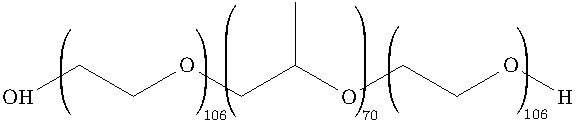
\includegraphics[scale=0.5]{Esquemas/f127.pdf} & \multirow{1}{*}{$13800$}	 & agente moldeante	 \\ \midrule
				  		  bromuro de hexadeciltrimetilamonio  CTAB   & \hspace*{1cm} 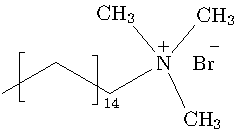
\includegraphics[scale=0.6]{Esquemas/ctab.pdf} & \multirow{1}{*}{$364.48$}	 & agente moldeante	 \\ \midrule
				  		  ácido clohídrico HCl& \includegraphics[scale=0.75]{Esquemas/hcl.pdf}  & \multirow{1}{*}{$36,46$}   & cataliza la hidrólisis \\ \midrule
				  		  agua \hspace{2cm} H$_2$O  &  \includegraphics[scale=0.75]{Esquemas/agua.pdf}  & \multirow{1}{*}{$18,02$}   & reactivo de hidrólisis \\ \midrule
				  		  etanol \hspace{2cm} EtOH  & \includegraphics[scale=0.75]{Esquemas/etanol.pdf}  & \multirow{1}{*}{$46,07$}   & solvente \\ 
				  		  \bottomrule
				    	  \end{tabular}
				   		  \label{tabla:reactivos}
					      \end{table}

			Una vez envejecida la solución de prehidrólisis (ya sea de SiO$_2$ pura o mixta) se agregan a \SI{17.146}{\gram} de esta, \SI{80.184}{\gram} de EtOH, \SI{3.246}{\gram} de F127 o \SI{1.822}{\gram} de CTAB y \SI{7.630}{\gram} de HCl \SI{2,5e-2}{\Molar}. De esta forma se obtienen unos \SI{100}{\ml} de un sol con las relaciones molares de la tabla \ref{tabla:soles}. Se conservan en \textit{frezeer} a \SI{-18}{\celsius} y solo se saca de allí a la hora de depositarlo. 

			Para facilitar la lectura se utilizará la siguiente nomenclatura, tanto para los soles como para las películas delgadas mesoporosas que se fabriquen con ellos: 

				\begin{itemize}
			 			\item \pdm\space para películas delgadas mesoporosas en general.
			 			\item \pdmF\space para \pdm\space de óxido de silicio estructuradas con F127 
			 			\item \pdmC\space para \pdm\space de óxido de silicio estructuradas con CTAB.
			 			\item \pdmZ\space para las \pdm\space mixtas de óxido de circonio y silicio en relación molar $1\!:\!9$ y estructuradas con F127. 
					    \end{itemize}	
			
				\begin{table}[ht]
			  		  \caption[Relación molares de los soles]{Relaciones molares para las soluciones utilizadas.} 
			  		  \begin{tabular}{>{\raggedright\arraybackslash}m{2.2cm}>{\centering\arraybackslash}m{2.2cm}>{\centering\arraybackslash}m{1.875cm}>{\centering\arraybackslash}m{1.875cm}>{\centering\arraybackslash}m{1.875cm}} 
			  		  \toprule
					  Componente & Prehidrólisis  & \pdmF   & \pdmC  & \pdmZ \\  \midrule
			      	  TEOS 		  & 1/0,9$^*$	  & 1   	& 1		 & 0,9   \\ \midrule
			      	  ZrCl$_4$	  & -/0,1$^*$	  &	-		& - 	 & 0,1   \\ \midrule	
			      	  EtOH 		  & 3			  & 40   	& 40	 & 40    \\ \midrule
			      	  F127 		  & -		 	  & 0,0075  & -		 & 0,0075\\ \midrule
			      	  CTAB 		  & -             & -		& 0,1	 & 0,1   \\ \midrule
			      	  H$_2$O	  & 1			  & 9	  	& 9	     & 9     \\ \midrule
			      	  HCl    	  & 0,00005		  & 0,01   	& 0,01	 & 0,01   \\ 
			      	  \bottomrule
			    	  \end{tabular}\vspace*{2pt}
		    	  	  \footnotesize{$^*$Los números después de la barra son los utilizados en soluciones de prehidrolisis para películas mixtas de silicio/circonio.}
			    	  \label{tabla:soles}
			   		  \end{table}
			Todas las soluciones fueron preparadas indistintamente en el Centro de Micro y Nanoelectrónica del Bicentenario del Instituto Nacional de Tecnología Industrial (INTI-CMNB) o en la Gerencia Química, Centro Atómico Constituyentes Comisión Nacional de Energía Atómica (CAC-CNEA). 
				
	\subsection{Depósitos de las películas delgadas mesoporosas}\label{sec:deposito_pdm}

			Las películas mesoporosas utilizadas en esta tesis fueron depositadas en el Laboratorio de Fotolitografía del INTI-CMNB por la técnica de \textit{spin-coating}. El equipo utilizado fue un \textit{Suss MicroTec Delta 20BM},  el cual consiste en un cabezal rotatorio con control de aceleración de 0 a  \SI{1000}{\minute^{-1}.\second^{-1}} y de velocidad variable de 0 a \SI{10000}{\minute^{-1}}; tiene varios portamuestras para sustratos de diferentes tamaños con entrada de vacío para sujetar las muestras (figura \ref{fig:spin}). 
			
			Se utilizaron como sustrato para depositar las \pdm, vidrio, silicio, oro sobre silicio, microelectrodos y sustratos poliméricos como  polimetilmetacrilato (PMMA) y poliestireno de alto impacto (PAI). Cada uno de ellos fue escogido para una función particular (p. ej. sustrato para reacciones electroquímicas) o por alguna característica distintiva (p. ej. transparente en el IR). En la tabla \ref{tabla:sustratos}, pág. \pageref{tabla:sustratos}, se agrupan los sustratos utilizados y se resumen algunas características y funciones destacadas.

			Las dimensiones de las muestras fueron típicamente de \SI{1x1}{\cm} a \linebreak \SI{2x2}{\cm}, aunque la técnica permite depositar películas continuas de hasta \SI{15}{cm} de diámetro. En algunos casos, para obtener un lote de sensores de más cantidad, se utilizaron obleas de silicio de \SI{10}{\cm} de diámetro. Antes de hacer el depósito, el sol se pasa a través de un filtro de jeringa de \SI{0.45}{\um} para evitar discontinuidades y/o <<cometas>> en los depositos\cite{Franssila2004}. Luego, para dispensar el sol en el sustrato, se utilizaron pipetas tipo Pasteur o pipetas automáticas dependiendo del volumen requerido, el cual varió de 80 a \SI{100}{\uL.\cm^{-2}}. Las condiciones del laboratorio durante el depósito se mantuvieron en \SI{25}{\celsius} y a una HR entre 30\% y 50\%. Una vez dispensado el sol, se da comienzo a la rotación que dispersa la solución de manera homogénea sobre el sustrato y, a su vez, la evaporación del solvente promueve la formación del cristal líquido por el mecanismo de autoensamblado molecular inducido por evaporación (EISA, del inglés \textit{evaporation induced self-assembly}) \cite{Brinker1999}.

					\begin{figure}[ht!]
					  \begin{center}
					  \includegraphics[width=\textwidth]{Imagenes/Spin.jpg}
					  \caption[Equipo para el depósito de películas delgadas, \textit{spin-coater}]{\textit{Spin-coater} ubicado en el Laboratorio de Fotolitografía del INTI-CMNB utilizado para el deposito de las películas delgadas mesoporosas, Marca \textit{Suss MicroTec}, modelo \textit{Delta 20BM}.}
					  \label{fig:spin}
					  \end{center}
					  \end{figure}

			El espesor de la película, ($t$), es inversamente proporcional a la raíz cuadrada de la velocidad angular ($\omega$), es decir $t\propto \omega ^{-1/2}$, por lo que las rampas de velocidad y aceleración utilizadas fueron optimizadas para lograr espesores entre 150 y \SI{300}{\nm}\cite{Meyerhofer1978,Hall1998,Brinker1990}. Los esquemas aplicados se muestran en gráfico de la figura \ref{fig:rampa-spin}. 
				
					\begin{figure}[!ht]
						 \begin{center}
						 \includegraphics[width=0.70\textwidth]{Graficos/rotacion_meso.pdf}
						 \caption[Parámetros de depósito para las \pdm]{Esquema con las rampas más frecuentes de aceleración, velocidad y tiempo utilizadas para el depósito de \pdm.}
						 \label{fig:rampa-spin}
						 \end{center}
						 \end{figure}

			 	    \begin{table}[ht!]
			  		   \caption[Sustratos utilizados para el depósito de \pdm]{Sustratos utilizados para el depósito de \pdm.} 
			  		   \begin{tabular}{>{\raggedright\arraybackslash}m{2.4cm}>{\raggedright\arraybackslash}m{2.5cm}>{\raggedright\arraybackslash}m{2cm}>{\raggedright\arraybackslash}m{3.55cm}} 
			  		   \toprule
					   Sustrato Nomenclatura   & Observaciones  & Limpieza previa$^*$ & Función \\ \midrule
			       	   vidrio \hspace{2cm} Vi  &	portaobjetos \textit{BioTraza} & inmersión KOH 40\% & económico para pruebas preliminares de deposito \\ \midrule
			       	   silicio\hspace{2cm} Si  & Si[100] pulido dopado tipo n  \textit{Addison}& inmersión HF 48\% & FTIR, SEM, FIB, EPA \\ \midrule
			       	   Au sobre silicio\hspace{2cm} Si$|$Au & depositado por pulverizacion catódica$^\dagger$  & ultrasonido en H$_2$O  & transporte, EQ\\ \midrule
			      	   microelectrodos \hspace{2cm} $\mu Elec$ & sensores, diseño transferido por fotolitografía$^\mathsection$  	  &  ultrasonido en H$_2$O  & multisensado, EQ \\ \midrule
			      	   polimericos         &  PMMA y PAI		  &  ultrasonido en H$_2$O &  demostrador métodos suaves de síntesis\\ 
			      	   \bottomrule
			    	   \end{tabular}\vspace*{2pt}
			    	   \footnotesize{$^*$Ver la sección <<\nameref{sec:limpieza}>>, tabla \ref{tabla:limpieza}, pág. \pageref{sec:limpieza}.}\\
			    	   \footnotesize{$^\dagger$Ver la sección <<\nameref{sec:sputt}>>, pág.\pageref{sec:sputt}.} \\
			    	   \footnotesize{$^\mathsection$Ver la sección <<\nameref{sec:fotolito}>>, pág. \pageref{sec:sputt}.}
			    	   \label{tabla:sustratos}
			   		   \end{table}
			
	\subsection{Eliminación del surfactante}\label{sec:cond_y_extr}

		Una vez realizado el depósito, se debe conservar la estructura del cristal líquido obtenido, y evitar el deterioro durante la eliminación del surfactante. Para ello se estabiliza la película durante \SI{1}{\hour} en cámara de humedad controlada a una HR constante de 50\%. Para mantener dicha humedad se utilizó una solución saturada de Ca(NO$_3$)$_2$.5H$_2$O (\textit{Biopack}). El ingreso de H$_2$O permite de esta forma aumentar el grado de polimerización del óxido y ayudar a la separación de fases entre el agente moldeante y el óxido\cite{Crepaldi2003}. El proceso de estabilización y condensación del óxido continua con un calentamiento en plancha calefactora, (\textit{Cimarec}) una hora a \SI{60}{\celsius} y una hora más a \SI{130}{\celsius}\cite{Crepaldi2003,Crepaldi2002a}. 
				
		Posteriormente a la estabilización de la película se experimentaron varios tratamientos para completar el proceso de condensación de la fase inorgánica y extraer el surfactante para dar lugar a la película nanoporosa, a saber:

				\begin{itemize}

				\item \textit{Calcinacion.} Este es el proceso clásico en el cual se somete a la película a una temperatura de \SI{350}{\celsius} durante \SI{2}{\hour} con una rampa de \SI{1}{\celsius.\minute^{-1}} (Horno \textit{Indef 337}). De esta forma se condensa el óxido, se elimina el surfactante y se minimiza el daño de la estructura tridimensional de la red nanoporosa \cite{Crepaldi2003}.

				\item \textit{Condensación ácida.} En este método se busca promover la condensación de la matriz inorgánica mediante la exposición de las películas a una atmósfera de vapores de HCl \cite{Doshi2000a}. El arreglo para tal fin consiste en sujetar las muestras al fondo de un vaso precipitados y colocarlo invertido sobre un cristalizador con HCl concentrado (\textit{Biopack}) durante \SI{10}{\minute}. 

				\item \textit{Condensación alcalina.} Al igual que el método anterior, se busca promover la condensación del óxido cambiando las condiciones del entorno químico, en este caso someter las películas a una atmósfera de pH extremadamente básico generada con vapores de NH$_3$ (\textit{Biopack}) \cite{Soler-Illia2012,Soler-Illia2011}. El armado experimental fue igual que el descripto para el método ácido.

				\item \textit{Tratamiento a \SI{130}{\celsius}.} Esta estrategia de síntesis involucró dejar las muestras en estufa a \SI{130}{\celsius} durante 7 días con el objetivo de promover la condensación del óxido.

				\item \textit{Alto vacío.} Este tratamiento consiste en dejar las muestras en una cámara de alto vacío a \SI{1e-5}{\milli\bar} y \SI{130}{\celsius} durante 7 días. Para calentar y llegar al vacío necesario se utilizó la cámara de una soldadura de obleas (\textit{EVG 501 Manual Wafer Bonding System}) la cual fue evacuada por una bomba mecánica y una turbomolecular secuencialmente.

				\end{itemize}
					
		En los casos donde fue necesario realizar la extracción del surfactante sin calcinar, las muestras fueron sometidas a un reflujo de isopropanol a punto de ebullición (\textit{Biopack}) durante \SI{15}{\minute}. Luego se enjuagaron con H$_2$O acidificada con HCl a $\text{pH}=2$. El siguiente diagrama de flujo resume y agrupa los tratamientos realizados sobre las \pdm, desde el depósito hasta la extracción del surfactante.
		
				\begin{figure}[ht!]
						  \begin{center}
						  \includegraphics[width=\textwidth]{Esquemas/Resumen_extraccion.pdf}
						  \caption[Tratamientos pos-depósito de \pdm]{Etapas de estabilización y diferentes tratamientos pos-depósito utilizados para hacer las \pdm, tanto de óxidos puros como las mixtas.}
						  \label{esq:peliculas_meso_tratamientos}
						  \end{center}
						  \end{figure}

	\subsection{Espectroscopia IR}\label{sec:IR}

		El segmento infrarrojo (IR) del espectro electromagnético puede ser divido en tres zonas, según su longitud de onda, IR cercano (400 a \SI{10}{\cm^{-1}}), IR medio (4000 a \SI{400}{\cm^{-1}}), e IR lejano (14000 a \SI{4000}{\cm^{-1}}). El infrarrojo medio puede ser usado para estudiar las vibraciones fundamentales y la estructura roto-vibracional; brinda información acerca de los grupos orgánicos e inorgánicos  presentes a través del análisis de las vibraciones moleculares.\cite{Atkins2006,Barrow1962,Stuart2004} 
		
		A lo largo de este trabajo se uso esta porción del espectro IR para analizar los resultados de la extracción de surfactante y estructura inorgánica de las \pdm. Las mediciones se llevaron a cabo en la Unidad Técnica de Nanomateriales del Centro de Investigaciones en Procesos Superficiales del INTI (INTI-CIEPS). El equipo es un \textit{Thermo Scientific Nicolet 6700 FTIR} que cuenta con un microscopio para poder focalizar el haz en un área de aproximadamente \SI{0.5x0.5}{\mm}. Se utilizó la técnica de espectroscopia infrarroja por transformadas de Fourier (FTIR) tanto en trasmisión como en reflexión y los espectros fueron tomados con el detector MCT/B (\textit{Wide Band mercury cadmium telluride}) que es de 4 a 10 veces más sensible que los detectores estándar para equipos de espectroscopia FTIR.\cite{Nicholet2007} Las películas destinada a ser caracterizadas por FTIR fueron depositadas sobre Si, por ser este trasparente en el IR medio.

	\subsection{Ángulo de contacto}

		La medición del angulo de contacto surge como una descripción teórica para el equilibrio entre tres fases; la fase líquida de la gota, la fase gaseosa del aire y la sólida del sustrato. El valor del ángulo de contacto depende principalmente de la relación que existe entre las fuerzas adhesivas entre el líquido y el sólido y las fuerzas cohesivas del líquido. Se puede, así, cuantificar la mojabilidad de un líquido en aire, en una determinada superficie.\cite{findenegg1997} Tomando dos caso extremos, cuando la superficie interactúa fuertemente con el líquido y se moja, el angulo de contacto se aproxima a $0^{\circ}$, en cambio si la superficie y el líquido se repelen, el angulo tenderá a $180^{\circ}$. En términos de equilibrio termodinámico, el potencial químico de las tres fases  debe ser igual. Quien dió la primera descripción en términos de energías interfasiales fue Young en 1805\cite{young1805}, donde postuló que la energía superficial líquido-vapor ($\gamma$) por el coseno del angulo de contacto($\theta$) es igual a diferencia de las energías superficiales sólido-líquido $\gamma_{_{SL}}$ y sólido-vapor  $\gamma_{_{SV}}$s. Tal relación se la conoce como ecuación de Young (ecuación \ref{eq:young}).

			\begin{equation}
				\gamma\, cos(\theta) = \gamma_{_{SL}} - \gamma_{_{SV}}
				\label{eq:young} 
				\end{equation}

		En este trabajo se utilizaron las medidas de angulo de contacto entre agua y las superficies de las \pdm, para calcular la distribución de los tamaños de poro y cuello de los sistemas porosos aplicando la ecuación de Kelvin.\cite{Boissiere2005} En la próxima sección se explica en detalle como se estiman dichas distribuciones.
		Las medidas de ángulo de contacto se realizaron en la Gerencia Química, CAC-CNEA con un equipo \textit{Ramé-Hart 290} y los datos fueron recogido con el software \textit{DROPImage}.

	\subsection{Elipsometría}\label{sec:elipso}

		La elipsometría es una técnica de análisis óptico que se basa en el cambio del estado de polarización de la luz que incide sobre una o más películas delgadas soportadas sobre un material reflectivo. Dicho análisis es no destructivo y es útil para la determinación de espesores y constantes ópticas (índices de refracción y constante de absorción) de dichas películas.\cite{TompkinsHarlandG.1999,Rothen1945} Las mediciones obtenidas nos devuelven los parámetros elipsométricos $\Delta(\lambda)$ y $\Psi(\lambda)$. 

		Mediante un modelo matemático (en el cual se proponen valores iniciales para las constantes ópticas y el espesor de la muestra) se ajusta por cuadrados mínimos hasta minimizar, por sucesivas iteraciones, la diferencia con los datos experimentales. De esta forma se extrae del modelo el espesor y el índice de refracción de la película. Cuando se adapta una cámara al equipo, donde se puede variar la presión parcial de H$_2$O, es posible medir los cambio de las propiedades ópticas de las \pdm durante la adsorción y desorción de H$_2$O. A esta técnica se la conoce con el nombre de porosimetría elipsométrica ambiental (PEA) \cite{Boissiere2005}. La figura \ref{fig:elipso} esquematiza el funcionamiento del elipsómetro y la figura \ref{fig:elipsofoto}, pág \pageref{fig:elipsofoto}, es una fotografía del equipo utilizado un \textit{SOPRA} modelo \textit{GES 5E}. 

			  \begin{figure}[t]
				\begin{center}
				\includegraphics[width=\textwidth]{Esquemas/Elipso.pdf}
			  	\caption[Esquema de la técncia de elipsoporosimetría ambiental]{Esquema de los componentes principales del equipos de elipsometría utilizado para determinar las constantes elipsométricas, $\Delta(\lambda)$ y $\Psi(\lambda)$, de las cuales se obtienen el espesor, indice de refracción, coeficiente de absorción, distribución y tamaño de poros y cuellos de las \pdm.}
			  	\label{fig:elipso}
			  	\end{center}
			  	\end{figure}
		
		El volumen de vapor adsorbido dentro de los poros se determina a partir de dicha variación utilizando aproximaciones de medio efectivo como la de Bruggeman\cite{Bruggeman1935} o la de Maxwell-Garnett\cite{Garnett1906} que son simplificaciones de la ecuación general de Lorentz-Lorentz\cite{TompkinsHarlandG.1999}.
		La aproximacion de Bruggeman considera dos componentes mezclados al azar cuyas fracciones en volumen ($f_i$) y constante dielectrica ($\mathcal{E}_i$) deben cumplir con la ecuación \ref{eq:bruggeman} donde $\mathcal{E}_e$ es la constante dieléctrica del material compuesto, la cual se determina experimentalmente.
							\begin{equation}
					 		   	 f_1\left(\frac{\mathcal{E}_1-\mathcal{E}_e}{\mathcal{E}_1+2\mathcal{E}_e}\right)+
					 		   	 f_2\left(\frac{\mathcal{E}_2-\mathcal{E}_e}{\mathcal{E}_2+2\mathcal{E}_e}\right)=0
					 		     \label{eq:bruggeman}
								\end{equation}
		La aproximación de Maxwell-Garnett considera al material compuesto por al menos dos especies, la matriz y la inclusión. En el caso de los óxidos porosos, la matriz es el óxido y el aire el surfactante la inclusión. Se deben satisfacer en este caso las ecuaciones \ref{eq:maxwall1} y \ref{eq:maxwall2}.
							\begin{equation}
					 		   	 f_1\left(\frac{\mathcal{E}_1-\mathcal{E}_2}{\mathcal{E}_1+1\mathcal{E}_2}\right)-
					 		   	 \left(\frac{\mathcal{E}_e-\mathcal{E}_2}{\mathcal{E}_e+2\mathcal{E}_2}\right)=0
					 		     \label{eq:maxwall1}
								\end{equation}
								\begin{equation}
					 		   	 f_2\left(\frac{\mathcal{E}_2-\mathcal{E}_1}{\mathcal{E}_1+2\mathcal{E}_1}\right)-
					 		   	 \left(\frac{\mathcal{E}_e-\mathcal{E}_1}{\mathcal{E}_e+2\mathcal{E}_1}\right)=0
					 		     \label{eq:maxwall2}
								\end{equation}
		El volumen total ocupado por los poros, V$_p$, y el volumen de agua adsorbido para cada HR, V$_{ads}$, se calcularon aplicando indistintamente dichas aproximaciones (ya que para \pdm\space dan resultados equivalentes) a las constantes dieléctricas medidas del film seco y lleno de agua, luego de la condensación capilar.\cite{Angelome2008,Fuertes2009,Nano-compuestas2013}. Se construye de esta forma una isoterma de adsorción/desorción de H$_2$O en función del índice de refracción de la o las películas porosas.
		El tamaño de los poros y los cuellos, que forman la red porosa tridimensional, se puede calcular a partir de la rama de adsorción y de la de desorción de la isoterma respectivamente. Para ello debemos recurrir a la ecuación de Kelvin (ec. \ref{eq:kelvin}), que describe el equilibrio líquido-vapor considerando tamaño de la esfera y energía superficial. Donde R es la constante de los gases, T es la temperatura, P es la presión de vapor, P$_s$ es la presión de vapor de saturación, $\gamma$ es la tensión superficial del líquido, V$_m$ es el volumen molar del líquido y $\theta$ es el ángulo de contacto sólido-líquido. \cite{Baklanov2000,Boissiere2005,Sing1985} Para poros esféricos la relación $\partial S/ \partial dV$ es proporcional al radio de la esfera, llamado radio de Kelvin.\cite{FernandezPrini2005}
			\begin{equation}
			  	 \ln \left(\frac{P}{P_s}\right)=\frac{2\gamma V_m}{RT} \cos{\theta}\frac{\partial S}{\partial V}
			     \label{eq:kelvin}
			 	 \end{equation}					
		Todas las medidas fueron tomadas en la Gerencia Química, CAC-CNEA con un elipsómetro espectroscópico marca \textit{SOPRA}, modelo \textit{GES 5E}. El rango espectral del equipo va de 190 a \SI{900}{\nm}, pose una cámara para realizar las mediciones en condiciones de humedad controladas y también permite configuración en modo \textit{micro-spot} que permite reducir el área de medición a una región de aproximadamente \SI{1}{\mm^2}. El modelado de los parámetros se hizo mediante el \textit{software Winelli II} también de la marca \textit{SOPRA}.
					\begin{figure}[ht]
							  \begin{center}
							  \includegraphics[width=\textwidth]{Imagenes/elipsometro.jpg}
							  \caption[Elipsómetro]{Foto del equipos elipsómetro espectroscópico marca \textit{SOPRA}, modelo \textit{GES 5E} ubicado en la Gerencia Química, CAC-CNEA utilizado para la caracterización de las \pdm.}
							  \label{fig:elipsofoto}
							  \end{center}
							  \end{figure}

\section{Microfabricación de los electrodos}
		
	 En esta sección se dará cuenta de los detalles experimentales para la fabricación de los electrodos, los cuales son una parte fundamental de los sensores. Es en la superficie de los electrodos donde se llevan a cabo las reacciones de óxido-reducción de los analitos de interés y donde se depositan la película delgada mesoporosa. Por estos motivos resulta fundamental contar con un diseño funcional y compacto y, además, controlar los aspectos superficiales tales como la rugosidad, control de impurezas, espesor, y funcionalización en los caso que sea necesario.

	 Los electrodos fueron enteramente diseñados y fabricados en los laboratorios del CMNB-INTI. 
		
	 Las herramientas y técnicas empleadas para la fabricación son propias del sector de la microelectrónica; herramientas de \textit{software} tipo CAD, fotolitografía, pulverización catódica, grabado por vía húmeda, \textit{lift-off}, corte y encapsulado, etc.\cite{Franssila2004,Jaeger2001} Cada uno de estos procesos y metodologías se explicarán en las secciones subsiguientes. 

	 El flujo general de trabajo para la transferencias de diseños en una o más capas se presenta en la figura \ref{esq:micro}.

			\begin{figure}[ht]
			  \begin{center}
			  \includegraphics[width=\textwidth]{Esquemas/Resumen_micro.pdf}
			  \caption[Esquema para la transferencia de diseños]{Diagrama general para la transferencias y fabricaciones de diseños de una o más capas. Este esquema contempla el uso de las técnicas de \textit{lift-off }o grabado según se requiera dependiendo de las características de los materiales empleados para esa capa.}
			  \label{esq:micro}
			  \end{center}
			  \end{figure}
			  
	\subsection{Diseño e impresión de las máscaras}\label{sec:impresion_mascaras}

		El primer paso necesario en la fabricación de los sensores es el diseño. Como todo diseño en microelectrónica, se pensó en función de las tecnologías disponibles, de la calidad de las máscaras y de la aplicación final en la cual se emplearán. Todos estos aspectos ya fueron expuestos en el capitulo \ref{chap:Introduccion}, por lo que aquí nos remitiremos a describir los detalles técnicos.

		Los diseño fueron pensaron para obleas de \SI{10}{\cm} de diámetro. El primer diseño se mandó a imprimir en filmina de \SI{13x13}{\cm} en una filmadora de películas \textit{Agfa Accuset 1000}, a una resolución de \SI{3600}{dpi}, perteneciente a la firma $Imacrom$. Esto ha permitido obtener resoluciones de linea de \SI{50}{\um}, muy por encima de la resolución de la tecnología de la cual disponemos (transferencia por UV, $\lambda=365nm$). El segundo diseño, mas completo e integrado, también fue diagramado para obleas \SI{10}{\cm} de diámetro. Este contempló la integración del contraelectrodo y el electrodo de referencia, además de incluir 6 electrodos de trabajo. Las máscaras correspondientes a este diseños se mandaron a imprimir en filminas de \SI{13x13}{\cm} a la empresa \textit{International Phototool Company} a una resolución de \SI{48000}{dpi}, logrando mejor resolución y lineas más definidas que en el primer diseño, hasta de \SI{7}{\um}. Todos los diseños se llevaron a cabo con el \textit{software CAD electric} (\url{http://www.staticfreesoft.com/productsFree.html}) de licencia pública general de GNU, \url{https://www.gnu.org/licenses/gpl.html}. 
				
	\subsection{Limpieza de los sustratos}\label{sec:limpieza}
			
			Una vez terminado el diseño, comienza la etapa de transferencia del mismo. El primer paso es la limpieza de los sustratos para evitar problemas de falta de adhesión y eliminar impurezas superficiales adsorbidas. 

			\begin{table}[!ht]
					  \caption[Soluciones para la limpieza de los sustratos]{Soluciones utilizadas para hacer la limpieza antes de realizar cualquier proceso de fotolitografía o pulverización catódica.\cite{Franssila2004,Kern1990}}
			  		  \begin{tabular}{>{\raggedright\arraybackslash}m{1.02cm}>{\centering\arraybackslash}m{2.8cm}>{\centering\arraybackslash}m{1.9cm}>{\centering\arraybackslash}m{1.9cm}>{\raggedright\arraybackslash}m{2.4cm}} 
			  		  \toprule
					  Nombre  & Composición &  Proporciones & Condiciones & Blanco \\ \midrule
			      	  KOH$^*$ & KOH:H$_2$O 	&    40\%p/v    &  \SI{25}{\celsius}/\SI{10}{\minute}  &  residuos orgánicos \\  \midrule
			      	  SC1$^\dagger$ &	H$_2$O:H$_2$O$_2$:NH$_4$OH & 5:1:1 & \SI{80}{\celsius}/\SI{10}{\minute} & residuos orgánicos  \\ \midrule
			      	  SC2 &	H$_2$O:H$_2$O$_2$:HCl & 6:1:1 & \SI{80}{\celsius}/\SI{10}{\minute}   &  residuos iónicos y metálicos \\ \midrule
			      	  HF  &	H$_2$O:HF & 50:1 & \SI{25}{\celsius}/\SI{2}{\minute} & óxido de silicio \\ \midrule
			      	  iPOH    &	  (CH$_3)_2$CHOH &  puro$^\mathsection$      &  enjuague & residuos grasos \\ \midrule
			      	  H$_2$O & H$_2$O desionizada & puro$^\ddagger$  &  enjuague  & desorción de partículas \\ \midrule
			      	  Piraña &  H$_2$SO$_4$:H$_2$O$_2$ & 2:1 & \SI{25}{\celsius}/\SI{10}{\minute}  & residuos orgánicos  \\
			      	  \bottomrule
			    	  \end{tabular}
			    	  \footnotesize{$^*$}No apta para silicio, racciona con el mismo para formar Si(OH)$_4$ e H$_2$. \\
				      \footnotesize{$^\dagger$}Crece una capa de SiO$_2$ de 10 a \SI{15}{\angstrom} de espesor. \\
				      \footnotesize{$^\mathsection$}Grado analítico o superior. \\
			    	  \footnotesize{$^\ddagger$}Resistividad de o \SI{18}{\mega\ohm\per\cm} o mayor.
			    	  \label{tabla:limpieza}
			   		  \end{table}
			
							
			La tabla \ref{tabla:limpieza} resume cuales fueron las soluciones utilizadas para limpieza, su composición y cuál es la finalidad de cada una. Al finalizar cada etapa de limpieza siempre se hace un lavado con H$_2$O DI seguido de un secado con aire o N$_2$. El porqué de los materiales elegidos para usar de sustratos ya fueron discutidos en el capitulo \ref{chap:Introduccion}, aquí solo se mencionan los protocolos de limpieza\cite{Franssila2004,Kern1990} utilizados para cada uno de ellos:

				\begin{itemize}
					\item{Vidrio: KOH}
					\item{Silicio: SC1, SC2, HF o piraña según el caso}
					\item{Sustratos poliméricos: ipOH}
				\end{itemize}

    \subsection{Transferencia de los diseños por fotolitografía}\label{sec:fotolito}

		La transferencia de los diseños se realizó por fotolitografía, técnica que también se conoce con los nombres de litografía óptica o litografía ultravioleta (UV). La técnica consiste en depositar una resina fotosensible sobre un sustrato, irradiar con luz UV de $\lambda\!=$\SI{365}{nm} a través de una máscara y por último revelar la fotorresina. Dependiendo si esta es negativa, positiva o de doble exposición, se disolverá la parte expuesta (positiva) o la no expuesta a la luz (negativa). \cite{Jaeger2001,Franssila2004,Mack2007,Mack2006}
	
		Antes de depositar la fotorresina se calienta el sustrato hasta \SI{120}{\celsius} con el objetivo de desorber H$_2$O. El depósito se realizó con el equipo descrito en la sección <<\nameref{sec:deposito_pdm}>>, pág. \pageref{sec:deposito_pdm}. Para cubrir una oblea completa de \SI{10}{\cm} de diámetro se necesitan colocar un mínimo de \SI{5}{\ml} de fotorresina \textit{TI35E image reversal} de la marca \textit{Microchemicals}, la cual es de doble exposición, especialmente elegida por formar un perfil negativo, particularmente útil para el proceso \textit{lift-off}, explicado mas adelante.\cite{MicrochemicalsTeam2009} 
			  \begin{figure}[ht]
			  \begin{center}
			  \includegraphics[width=0.60\textwidth]{Esquemas/fotolito.pdf}
			  \caption[Esquema fotolitografía]{Proceso de fotolitografía para una resina de doble exposición. 1) Deposito de la resina, 2) Calentamiento suave, mejora la adherencia y evapora solventes, 3) 1$a$ exposición, 4) Calentamiento para invertir la polaridad de la resina, 5) 2$a$ exposición sin máscara, 6) Revelado, notese el perfil invertido, especialmente útil para aplicar en procesos de\textit{ lift-off}.}
			  \label{esq:fotolito}
			  \end{center}
			  \end{figure}			  
		El deposito se hizo por \textit{spin-coating}, a una velocidad final de \SI{4000}{\minute^{-1}} durante \SI{40}{\second}, con una aceleración de \SI{400}{\minute^{-1}.\second^{-1}} para obtener un espesor final de \SI{4}{\um}. Luego se realiza un calentamiento durante \SI{2}{\minute} a \SI{95}{\celsius} para evaporar el exceso de solvente y promover la adhesión de la resina al sustrato. Seguidamente se cargan el sustrato y la máscara en la alineadora de máscaras (\textit{EVG 620}, figura \ref{fig:alineadora}), la cual cuenta con un microscopio incorporado para hacer la alineación máscara/sustrato y una lámpara de Hg para el sistema de irradiación UV. 

		Después de alinear, se realiza la primera exposición con un densidad de energía de \SI{140}{mJ.\cm^{-2}} y se deja reposar \SI{10}{\minute} para dar tiempo a la difusión de N$_2$ liberado durante la reacción. Se realiza ahora el calentamiento para invertir el perfil (las zonas expuestas polimerizan volviéndose inerte al solvente) de la resina a una temperatura de \SI{120}{\celsius} durante \SI{2}{\minute}  y se expone por segunda vez a una densidad de energía de \SI{540}{mJ.cm^{-2}},
		
		esta vez sin máscara. En esta segunda exposición las partes polimerizadas no se afectan, mientras las no expuestas en la primera iluminación se vuelven solubles en el medio revelador. Para finalizar, se hace el revelado surmegiendo la oblea en un cristalizador con una solución de revelador \textit{AZ General} (\textit{Microchemicals}) y H$_2$O 1:1. La evolución del revelado se siguió mediante microscopía óptica y se determinó en aproximadamente unos \SI{7}{\minute}, dependiendo del espesor de la fotoresina. De esta forma quedan transferidos los diseños. El flujo de trabajo se sintetiza en el esquema \ref{esq:fotolito}.

			\begin{figure}[ht]
			  \begin{center}
			  \includegraphics[width=\textwidth]{Imagenes/alineadora.jpg}
			  \caption[Alineadora de máscaras]{Alineadora de máscaras \textit{EVG 620} semiautomática de doble cara, con lámpara de Hg de \SI{350}{W}  y capacidad para obleas de hasta \SI{150}{\mm} .}
			  \label{fig:alineadora}
			  \end{center}
			  \end{figure}	

	\subsection{Depósito películas delgadas metálicas}\label{sec:sputt}

			En esta sección se describe el modo en que fueron fabricadas las películas delgadas de Au cuya función es ser usadas como electrodos en los sensores. 
				  \begin{figure}[t!]
				  \begin{center}
				  \includegraphics[width=\textwidth]{Imagenes/sputt.jpg}
				  \caption[Equipo para depósito de películas delgadas, \textit{sputtering}]{Foto del instrumental utilizado para realizar los depósitos bicapa Ti\textbar Au o Cr\textbar Au. A)El equipo \textit{BOC Edwards} completo donde se ve el gabinete de control y la cámara de vacío, B)Foto a través de la ventana al momento de realizar un deposito de Cr y C)Foto a través de la ventana al momento de realizar un deposito de Au.}
				  \label{fig:sputt}
				  \end{center}
				  \end{figure}	
			
			Para su fabricación se utilizó la técnica de pulverización catódica, la cual es comúnmente conocida por su nombre en ingles, \textit{sputtering}\cite{sigmund1968}. Los fundamentos básicos de la técnica se discutieron en el capitulo \ref{chap:Introduccion}, pág. \pageref{sec:microfabricacion}.

			Se utilizaron como sustratos de los electrodos principalmente obleas de silicio monocristalinas (vírgenes o fotolitografiadas) y portaobjetos de vidrio.  Estos soporte fueron escogidos debido la baja rugosidad de su superficie y por ser materiales que pueden ser sometidos a temperaturas altas, en particular \SI{350}{\celsius}, que es la temperatura de calcinación para la ruta de síntesis clásica de óxidos mesoporosos. Previo a realizar el depósito, los sustratos fueron tratados con los procesos de limpieza descritos en la sección \ref{sec:limpieza}, pág. \pageref{sec:limpieza} y una vez dentro de la cámara se realizó una limpieza por plasma para promover una mayor adherencia del depósito al sustrato.

			Cabe destacar que si se trabaja sobre obleas de silicio, estas tienen que estar recubiertas con una capa dieléctrica para que no haya fugas eléctricas a través del silicio. A lo largo de este tesis se utilizó indistintamente obleas que ya venían con capa aislante u obleas a las cuales se le depositó una película delgada de SiO$_2$, también por pulverización catódica.

			Para promover la adherencia del Au, se deposita una capa de al menos \SI{20}{\nm} de espesor, la misma puede ser indistintamente de Ti o Cr. Sin esta capa el Au no adhiere sobre superficies no metálicas\cite{Hieber1976}. Una vez depositada esta capa de adherente y sin romper el vacío de la cámara del equipo, se depositan un mínimo \SI{150}{\nm} de Au, para lograr un electrodo mecánicamente robusto y con buenas propiedades de conducción eléctrica. En los casos que se depositó una capa dieléctrica de SiO$_2$ se utilizó la fuente de radiofrecuencia (RF) a potencia constante, P=\SI{400}{W}. Mientras que los depósitos de las películas metálicas se realizaron todos con la fuente de corriente directa (DC) también configurada a P=\SI{400}{W}, dejando la tensión y la corriente libre, parámetros que dependen a su vez del vacío en la cámara, de la distancia entre el cátodo y el ánodo y el caudal de argón. Para cada caso, en condiciones constantes, se puede realizar una curva de calibración. La misma se construye graficando el espesor de las películas depositadas en función del tiempo de depósito, con el objetivo de establecer la tasa de depósito para cada material. 

			Las condiciones de depósito de cada una de las sucesivas capas se detallan en la tabla \ref{tabla:sputt1} para las películas metálicas y en la tabla  \ref{tabla:sputt2} para el SiO$_2$ y el plasma previo al deposito.

			%Tabla con los parámetros de deposito de la películas
		  		\begin{table}[ht]
		  		\caption[Parámetros de depósito películas metálicas]{Parámetros de depósito de las distintas películas delgadas metálicas para su uso como electrodos de trabajo.}
		  		\begin{tabular}{lcccccc} 
		  		\toprule
		    	 Depósito&$P_{_{\text{DC}}}$(W) & $T$(V)  &  $I$(A)   & $p$(mbar) & $Q_{Ar}$(sccm)   & $T$(nm/min) \\
		    	 		\midrule
		  		 Ti 	 & $400$ & $750$ & $0.53$ & \num{1.70e-3} & $5$ & $50$ \\
		  		 Cr 	 & $400$ & $453$ & $0.84$ & \num{1.70e-3} & $5$ & $55$ \\
		  		 Au 	 & $400$ & $679$ & $0.56$ & \num{1.35e-3} & $5$ & $44$ \\
		    	 \bottomrule
		    	 \end{tabular}
		   		\label{tabla:sputt1}
		   		\end{table}
		   		
		  		\begin{table}[ht]
		  		\caption[Parámetros de depósito películas dieléctricas]{Parámetros de depósito utilizado para el depósito de $SiO_2$.}
		  		\begin{tabular}{lccccc} 
		  		 		\toprule
		       	Depósito&$P_{_{\text{RF}}}$(W)  &$P_{ref}$(W)  &$p$(mbar) & $Q_{Ar}$(sccm) &$T$(nm/min)\\
		    	 		\midrule
		  		 $SiO_2$  & $400$ & $23$ & \num{1.23e-2} & $80$ & $1.18$ \\
		  		 Limpieza & 150   & 3    & \num{2.04e-3} & 10   & -      \\
		  		\bottomrule
		  		\end{tabular}
		   		\label{tabla:sputt2}
		   		\end{table}
		   	
		   	Todos los depósitos fueron realizados en el equipo de \textit{sputtering} del INTI-CMNB. El mismo cuenta, entre sus principales capacidades, con una fuente DC (hasta \SI{1.5}{\kW}) una fuente de RF (\SI{600}{W} a \SI{13.56}{\MHz}), posibilidad de depositar 3 materiales consecutivamente y capacidad para colocar sustratos de hasta \SI{250}{\nm}. El mismo es de la marca \textit{Boc Edwards}, en la figura \ref{fig:sputt} se muestra el equipo y un detalle al momento de hacer los depósitos.

	\subsection{Proceso de\textit{ lift-off}}
			Una vez finalizados los procesos de fotolitografía y pulverización catódica del metal o de los metales necesarios queda sólo remover la resina.

					\begin{figure}[!ht]
							  \begin{center}
							  \includegraphics[width=\textwidth]{Esquemas/liftoff.pdf}
							  \caption[Esquema del proceso de\textit{ lift-off}]{Esquema del proceso de\textit{ lift-off} en el cual se solubiliza la fotorresina con película metálica encima. 1) Fotorresina transferida en base a un diseño arbitrario, 2) depósito metálico, 3) disolución de la fotorresina con un solvente adecuado, 4) Diseño completamente trasferido.}
							  \label{esq:liftoff}
							  \end{center}
							  \end{figure}

		 La bicapa Ti\textbar Au o Cr\textbar Au se pulverizó sobre toda la superficie de la oblea, tanto en las partes donde estaba el silicio descubierto como en las partes donde quedó la fotorresina sin revelar. 
			
		 De esta forma, al estar el metal sobre la resina, disolviendo ésta, se desvincula la capa Ti\textbar Au del sustrato y queda completa la transferencia de los diseños. 
		 La disolución de la fotoresina se lleva a cabo en acetona (\textit{Sigma}) dentro de un baño de ultrasonido (\textit{TESTLAB} Modelo \textit{tb02}) a \SI{22}{\kHz}. En la figura \ref{esq:liftoff} se esquematiza todo el proceso completo.

	\subsection{Modificación superficial}\label{sec:silanizacion}
		
		A lo largo del trabajo surgió la necesidad de mejorar la adherencia de las \pdm\space sobre los electrodos de Au. Para lograr ésto, se realizó sobre los electrodos una modificación superficial, de forma de generar puntos de anclaje para promover la adherencia del óxido de silicio sobre la superficie de los electrodos.
		El proceso consistió en vincular covalentemente una molécula a la superficie de Au y, por otro lado, que ésta misma molécula sea parte estructural de las \pdm. Para lograr ésto se preparó una solución \SI{10}{\milli\Molar} de 3-mercaptopropil trimetoxisilano (MPTMS) en tolueno (se eligió tolueno de forma de minimizar la hidrólisis y condensación del MPTMS) y se dejo reaccionar durante 2 horas en cristalizador. \cite{Goss1991,Herzog2013} Luego se realiza un enjuague con acetona y se seca en flujo de N$_2$.

	\subsection{Encapsulado y corte}\label{sec:corte}

		Sobre los electrodos depositados se deposita una resina negativa, epoxi y fotocurable, \textit{SU8-100} de \textit{MicroChemical}\cite{MicrochemicalsTeam2009}. Dicha resina es ópticamente transparente y de alta viscosidad, lo que permite generar capas de hasta \SI{100}{\um} de espesor. 

		Fue utilizada con un doble propósito, proteger mecánicamente los sensores y hacer un reservorio o celda con un volumen  $V \approx$ \SI{2}{\ul}, el cual contendrá la solución con los analitos que se desean detectar.  
			%Graficos de rampa de velocidades		  
			\begin{figure}[ht]
			 		  \begin{center}
			 		  \includegraphics[width=0.70\textwidth]{Graficos/rotacion_su8.pdf}
			 		  \caption[Parámetros de depósito para la resina epoxi]{Esquema de aceleración y velocidad de rotación para el depósito de la fotorresina epoxi SU8.}
			 		  \label{fig:spin-su8}
			 		  \end{center}
			 		  \end{figure}
	
		Para controlar el espesor mediante \textit{spin-coating} se utilizó el esquema de rotación que de la figura \ref{fig:spin-su8}. Luego se realizó un secado para evaporar solventes a \SI{65}{\celsius} durante \SI{1}{\minute} y \SI{95}{\celsius} durante \SI{10}{\minute}. Seguidamente, se expone al UV a través de la máscara con una densidad de energía de \SI{680}{mJ.cm^{-2}}, para activar los iniciadores de la polimerización sólo en las zonas iluminadas. Se realiza un segundo calentamiento gradual de \SI{1}{\minute} a \SI{65}{\celsius} y \SI{12}{\minute} a \SI{95}{\celsius} para incrementar el grado de polimerización y finalmente se lleva a cabo el revelado (revelador para resina SU-8 de \textit{MicroChemical}), el cual requiere un tiempo de \SI{10}{\minute} para disolver completamente las partes que no fueron expuestas a la luz UV. 
		
		Para concluir la fabricación de los sensores se corta la oblea en cuadrados de \SI{1x1}{\cm} con el próposito de obtiener así cada dispositivo individual con 6 electrodos de trabajo cada uno. El corte se realiza con un disco de carburo de silicio de  de la marca \textit{Loadpoint} girando a \SI{44000}{\minute^{-1}} y con una velocidad de avance de \SI{1}{\mm}. El mismo fue montado en una cortadora de obleas marca \textit{Laser Optics} ubicada en los laboratorios del INTI-CMNB (ver figurea \ref{fig:dicer}).
			\begin{figure}[ht]
			 		  \begin{center}
			 		  \includegraphics[width=\textwidth]{Imagenes/dicer.jpg}
			 		  \caption[Cortadora de obleas]{Cortadora de obleas de la marca \textit{Laser Optics}.}
			 		  \label{fig:dicer}
			 		  \end{center}
			 		  \end{figure}

	\subsection{Espectroscopia de fotoelectrones de rayos X}

		La técnica de XPS (del ingles, \textit {X-ray photoelectron spectroscopy}) es una espectroscopia semi-cuantitativa y de baja resolución espacial que habitualmente se utiliza para estimar la estequiometría, estado químico de oxidación de algún elemento en particular y la estructura electrónica de los elementos en superficie.\cite{siegbahn1956,siegbahn1981}

		Se hizo uso de esta técnica para evaluar estados de oxidación del Au y comprobar difusión de contaminantes hacia la superficie de los electrodos.  Los equipos constan de diferentes componentes; una cámara de ultra alto vacío (UHV) con presiones del orden de \SI{1e-9}{mbar} para disminuir la cantidad de contaminantes superficiales y asegurar a los electrones eyectados un camino libre medio lo suficientemente grande como para alcanzar el analizador. La cámara está construida en acero inoxidable y posee ventanas de vidrio para poder observar su interior. A ella se acoplan diferentes elementos necesarios para el análisis superficial como la fuente de rayos X, el analizador de electrones, el cañón de iones, entre otros.\cite{XPS1978,Corthey2012}

		Las medidas de XPS realizadas se llevaron a cabo en el Instituto de Investigaciones Fisicoquímicas Teóricas y Aplicadas (INIFTA). Se utilizó una fuente de Mg K$\alpha$ (\textit{XR50, Specs GmbH}) y un analizador hemisférico (\textit{PHOIBOS 100, Specs GmbH}). La presión dentro de la cámara de UHV fue menor a \SI{1e-9}{mbar} mbar. El ángulo entre la fuente de rayos X y el eje del analizador está fijado en \ang{54;44;00}. Los valores de sección eficaz de fotoionización están tabulados para esta geometría. Se realizó una calibración de la escala de energía de dos puntos utilizando Au evaporado ($E_B$ de Au$f_{7/2}$ = \SI{84}{\electronvolt}) y Cu ($E_B$ de Cu $2_{p3/2}$ = \SI{932.67}{\electronvolt}).
		
\section{Microscopías}
		
	 En este apartado haremos un breve resumen de los tipos de microscopía utilizadas durante la tesis.

	\subsection{Microscopía óptica}

		Se utilizó microscopia óptica en modo reflexión fundamentalmente para evaluar la superficie (homogeneidad, fracturas, grietas, etc), tanto de las películas metálicas como de las mesoporosas. También para determinar la calidad de las máscaras impresas y para establecer los tiempos de revelado en los procesos fotolitográficos. Se utilizó un microscopio \textit{Olympus} modelo \textit{BX51} configurado tanto para trasmisión como para reflexión. Como fuente de luz el equipo cuenta con lámpara halógena y, en los casos que hizo falta, se intercaló un filtro ultravioleta de forma de no exponer las fotorresinas durante la inspección y evaluación de los tiempos de revelado.
	
	\subsection{Microscopía electrónica de barrido (MEB)}\label{sec:SEM}

		La microscopia electrónica de barrido (MEB) nos permitió ver y caracterizar las películas delgadas, ya sean los electrodos o las \pdm. Tamaño de poro, homogeneidad, tamaño de cristales, microfisuras y espesores son algunas las características que se pudieron evaluar con esta técnica. Además, el equipo utilizado nos permitió hacer análisis por espectroscopia de rayos X dispersiva en energía (EDS, del inglés \textit{Energy Dispersive Spectroscopy}) y tomar imágenes tanto con electrones secundarios como con electrones retrodifundidos. \cite{Goodhew2000,Watt1997}

		Se utilizó un microscopio de la marca \textit{FEI}, modelo \textit{Helios NanoLab 650} equipado con dos columnas, una de iones de galio y otra de electrones. Dejaremos la explicación de la microsopía de iones de Ga para la siguiente sección. La fuente de la columna de electrones es un emisor tipo FEG (del ingles \textit{Field Emission Gun}) y como instrumental de detección cuenta con detector de electrones secundarios (SE, del ingles \textit{Secondary Electron}), de electrones retrodifundidos (BSD, del ingles \textit{back scatter detector}) y de inmersión (TLD, \textit{Thought Lens Detector}), ver esquema presentado en la figura \ref{fig:sem-fib}. 

		Se utilizaron tensiones de trabajo bajas típicamente entre \SI{1}{\kilo\electronvolt} y \SI{5}{\kilo\electronvolt} e intensidades del orden de los \SI{25}{\pA}. La justificación de estos valores es que al acelerar los electrones con bajas tensiones la penetración en la muestra es pobre. Si bien depende del tipo de material, podemos estimar en base simulaciones de trabajos en la literatura especializada que, para oro o silicio, la penetración con los valores de tensión citados es de unos 50 a \SI{200}{\nm} \cite{Joy1984,Shur2012,Hafner2007}. Por el otro, se utilizo un flujo de electrones también bajo (\SI{25}{\pA}), de manera de evitar el apantallamiento debido a la acumulación de carga superficial en la muestra. Todos las imágenes de MEB en este trabajo incluyen las condiciones experimentales utilizadas en la barra de escala situada debajo de cada una de ellas.

	\subsection{Microscopía con iones de galio focalizados (FIB)}\label{sec:FIB}

		El bombardeo con haz de iones (FIB, del ingles \textit{focused ion beam}) es una técnica que se utiliza fundamentalmente para el análisis de materiales en general y en particular materiales de la industria de la microelectrónica, más específicamente para análisis de microsistemas (MEMS, del ingles \textit{Micro Electro Mechanical Systems}) y circuitos integrados (IC, del ingles \textit{Integrated Circuits}).

			\begin{figure}[ht]
			 		  \begin{center}
			 		  \includegraphics[width=\textwidth]{Imagenes/sem-fib.jpg}
			 		  \caption[Microscopio de doble haz FIB/SEM]{Equipo de FIB/SEM utilizados para realizar las observaciones, cortes y caracterizaciones de los sensores. Consta de un microscopio de barrido electrónico de alta resolución y de una fuente de galio líquido para realizar, entre otras cosas, cortes en la micro y nanoescala.}
			 		  \label{fig:sem-fib}
			 		  \end{center}
			 		  \end{figure}

		Consiste en el bombardeo de iones de galio para desplazar los átomos de la muestras. El Ga$^{\circ}$ (que se almacena en en un reservorio en la cabeza de la columna) se licua y se ioniza para dar lugar a los iones de Ga${^+}$, los cuales mediante un sistema de lentes magnéticas (similar al usado en MEB)  aceleran y focalizan los iones sobre la muestra. 

		\begin{figure}[ht!]
			 		  \begin{center}
			 		  \includegraphics[width=0.60\textwidth]{Esquemas/sem-fib.pdf}
			 		  \caption[Esquema de las microscopias FIB/SEM]{Esquema donde se muestra la disposición de las columnas de electrones y de átomos de galio del \textit{Helios NanoLab 650} y los principales eventos que ocurren al impactar los haces con la muestras.}
			 		  \label{esq:sem-fib}
			 		  \end{center}
			 		  \end{figure}

		El impacto de los mismos desplaza los átomos de la muestra generando así <<cortes>> sobre la muestra. Previo al impacto se deposita sobre la muestra una delgada capa de Pt ($\sim$\SI{150}{\nm}) para protección de la muestra y generar un borde de corte mas abrupto, ya que la taza de desplazamiento de los átomos de Pt con iones Ga${^+}$ es baja.\cite{Giannuzzi2005,Orloff1996} La técnica es de especial utilidad para examinar secciones transversales de muestras, calcular espesores, reconstruir volumenes en 3D, preparar láminas para microscopia electrónica de trasmisión, entre otros tantos ejemplos. El haz de iones se utiliza en la mayoría de los casos a \SI{30}{\kilo\electronvolt}. En el esquema \ref{esq:sem-fib} se muestra como es la disposición de las columnas y en la figura \ref{fig:sem-fib} una foto del equipo utilizado ubicado en los laboratorios del INTI-CMNB.\cite{Orloff2003,Reyntjens2001}

\section{Mediciones Electroquímicas}\label{sec:medidas_eq}
		
			Las mediciones electroquímicas fueron una parte central de este trabajo. Se utilizaron dos tipos de técnicas voltamperométricas, de corriente continua y de corriente alterna. No solo se hizo uso de ellas como técnicas analíticas sino también como herramienta para establecer parámetros de transporte, concentración dentro y fuera de los poros, calcular constantes de difusión y e inferir mecanismos de transporte de las sondas a través de la red nanoporosa. 

			Se utilizó, para ambas técnicas la típica configuración de celda de tres electrodos. La celda en sí fue fabricada en acrílico, con un volumen aproximado de \SI{3}{\ml} y con un orificio en la parte inferior. Para sellar contra el sustrato y evitar perdidas de la solución, se utilizo un sello de \SI{1}{\mm} de radio, el cual determina el área geométrica utilizada en \SI{3.15}{\mm^{2}}. En la figura \ref{fig:celda} se muestra un esquema del sistema de medición EQ y en la figura \ref{esq:eq} una fotografía de una de las tantas mediciones realizadas. 

			 \begin{figure}[!ht]
			 		  \begin{center}
			 		  \includegraphics[width=\textwidth]{Esquemas/celda.pdf}
			 		  \caption[Configuración de una celda de tres electrodos]{Configuración de de una celda tres electrodos para realizar medidas electroquímicas.}
			 		  \label{fig:celda}
			 		  \end{center}
			 		  \end{figure}

	 		 \begin{figure}[ht!]
			 		  \begin{center}
			 		  \includegraphics[width=\textwidth]{Imagenes/eq.jpg}
			 		  \caption[Equipo para realizar la medidas electroquímicas]{Fotografía del instrumental que se utilizó a lo largo de la tesis para tomar las medidas electroquímicas.}
			 		  \label{esq:eq}
			 		  \end{center}
			 		  \end{figure}	
			 		  
			Las mediciones electroquímicas fueron tomadas con un potencionestato \textit{Teq4}, para las medidas que se necesitaron velocidades de barrido mayores a \SI{1}{\volt\per\second} se uso un \textit{Autolab}, de la firma \textit{Ecochemie}. Como electrodo de referencia se utilizó un electrodo saturado de calomel (ESC) de la firma \textit{Cole-Parmer} y como contraelectrodo (CE) se utilizaron indistintamente electrodos de Au depositados por pulverización catódica o una pieza de Pt de tamaño adecuado. En la tabla \ref{tabla:eq} se resumen los reactivos utilizados para llevar a cabo las mediciones electroquímicas. 
			
			A continuación se hace una breve reseña sobre las técnicas utilizadas, los parámetros empleados y las configuraciones experimentales.

			 \pagebreak

				%Tabla ractivos EQ
				     \begin{table}[ht!]
			  		  \caption[Reactivos utilizados para las mediciones electroquímicas]{Reactivos y sondas electroquímicas utilizados para las mediciones electroquímicas}
			  		   \begin{tabular}{>{\raggedright\arraybackslash}m{4.4cm}>{\centering\arraybackslash}m{1.75cm}>{\centering\arraybackslash}m{2.7cm}>{\raggedright\arraybackslash}m{1.6cm}} 
			  		  \toprule
					  Reactivo \hspace{3cm}Nombre& Marca & Peso Molecular (\si{g.mol^{-1}}) & Función  \\ \midrule
			    	  \ferroCompleto \hspace{3cm} ferrocianuro de potasio & \textit{Sigma} & 422,41  & Sonda \\ \midrule
			    	  \ferriCompleto \hspace{3cm} ferricianuro de potasio & \textit{Sigma} & 329,27  & Sonda  \\ \midrule
			  		  \aminorutenioCompleto  \hspace{3cm}  cloruro de hexaaminorutenio& \textit{Aldrich} &  309,61  & Sonda  \\ \midrule
			  		  \raisebox{-.5\height}{\includegraphics[scale=0.4]{Esquemas/Fc.pdf}}  \hspace{3cm} ferroceno metanol   & \textit{Aldrich} &  216,06 & Sonda  \\ \midrule
			  		  \raisebox{-.5\height}{\includegraphics[scale=0.4]{Esquemas/HQ.pdf}} \hspace{3cm} hidroquinona	& \textit{Biopack} & 110.11  & Sonda  \\ \midrule
			  		  H$_2$O \hspace{3cm} agua &  \SI{18}{\mega\ohm\per\cm}  &  18,02 & Solvente \\ \midrule
			  		  KCl  \hspace{3cm} cloruro de potasio   & \textit{Biopack} & 74,56 & Electrolito Soporte \\
 			  		  \bottomrule
			    	  \end{tabular}
			   		  \label{tabla:eq}
			   		  \end{table}

	 \subsection{Voltametría cíclica}
	 		
	 		La voltamperometría cíclica (VC) consiste en variar, de una manera cíclica, el potencial de un electrodo estacionario contra un electrodo de referencia. Ambos se encuentran inmersos en una solución en reposo y se mide la corriente resultante entre ellos. La señal de excitación es un barrido de potencial lineal con una onda de forma triangular, la cual parte de un potencial E$_1$, evoluciona linealmente hasta un potencial E$_2$ para luego volver a E$_1$. Las velocidades de este barrido pueden variar desde unos cuantos milivolts por segundo hasta cientos de volts por segundo; en nuestro caso se utilizaron velocidades próximas a los \SI{50}{\milli\volt.\second^{-1}}, se escogieron estas velocidades para llevar a cabo experimentos de una duración aceptable pero donde aún predomine la transferencia de carga y no se observe desplazamiento de potenciales para los picos de máxima oxidación y/o reducción.\cite{nicholson1964,Gewirth2004}

	 		Como ya se dijo anteriormente se barre el potencial del electrodo de trabajo en dirección de ida y vuelta entre dos valores arbitrarios, E$_1$ y E$_2$. Al usar soluciones en base acuosa se debe trabajar en la región de estabilidad electroquímica del H$_2$O, para evitar reducción u oxidación de la misma, que genera H$_2$ u O$_2$ respectivamente. En la gran mayoría de los experimentos presentados en este trabajo se trabajo en un pH$\sim 5$ para el cual el rango de estabilidad del agua es entre \SI{-0.5}{\volt} y \SI{0.7}{\volt}, usando como referencia un electrodo saturado de calomel.\cite{wang2014} 

	 		En la figura \ref{fig:CV_ideal} se muestra la onda triangular de excitación aplicada y la curva obtenida para una sonda electroquímica idealmente reversible, donde se destacan los parámetros mas importantes.
	 			 \begin{figure}[ht]
			  		  \begin{subfigure}[t]{0.495\textwidth}
			  		  \includegraphics[width=\textwidth]{Graficos/onda-triangular.pdf}
			  		  \end{subfigure}
			  		  \begin{subfigure}[t]{0.495\textwidth}
			  		  \includegraphics[width=\textwidth]{Esquemas/CV-ideal.pdf}
			  		  \end{subfigure}
			  		  \caption[Voltamperometria ideal reversible]{Curva de excitación y voltagrama típico para una especie redox reversible.}
			  		  \label{fig:CV_ideal}
			  		  \end{figure}

	 		Esta técnica se utilizó para evaluar fenómenos de exclusión, permeación y preconcentración. También para determinar concentración de las sondas electroactivas dentro y fuera de los poros, calcular coeficientes de difusión y estimar distancias de sitios redox así como chequear accesibilidad y estructura de las películas delgadas mesoporosas.

	 \subsection{Voltametría cíclica de corriente alterna}

	 		La técnica de voltametría cíclica de corriente alterna (VCA) consta en aplicar una oscilación sinusoidal de voltaje a la celda electroquímica. A la onda triangular clásica usada en VC se la perturba, montando sobre ella, una pequeña onda de corriente alterna, en los experimentos presentados en este trabajo la perturbación fue de de \SI{10}{\milli\volt} y la frecuencia de la misma de 1 y \SI{2}{\hertz}. Esta técnica se emplea en conjunto con un analizador de frecuencias para filtrar la componente continua de la alterna, de este modo, ofrece un limite de detección menor e incrementa la sensibilidad respecto de la CV tradicional.\cite{Wi2000,Skoog1995}

	 		En la figura \ref{fig:ACV_ideal} se muestra la onda triangular con la perturbación, y la curva obtenida para una sonda electroquímica idealmente reversible, luego del filtrado de la componente continua.

	 			 \begin{figure}[ht]
			  		  \begin{subfigure}[t]{0.495\textwidth}
			  		  \includegraphics[width=\textwidth]{Graficos/onda-triangular-sin.pdf}
			  		  \end{subfigure}
			  		  \begin{subfigure}[t]{0.495\textwidth}
			  		  \includegraphics[width=\textwidth]{Graficos/ACV-ideal.pdf}
			  		  \end{subfigure}
			  		  \caption[Voltamperometria ideal reversible]{Curva de excitación y voltagrama típico para una especie redox reversible.}
			  		  \label{fig:ACV_ideal}
			  		  \end{figure}
	 		
	 		El propósito de esta técnica fue el obtener el coeficiente de difusión de hexaaminorutenio en sistemas porosos y contrastar con otras técnicas de forma de validar dicho coeficiente y los mecanismos de trasporte propuestos. 

	 \subsection{Simulaciones electroquímicas}\label{simulacion}

	 	 Para validar las hipótesis de transporte planteadas en el capitulo \ref{chap:Electroquimica} se llevaron a cabo simulaciones por computadora para voltametrías cíclicas. Las mismas se hicieron con el software  \textit{COMSOL Multiphysics\textsuperscript\textregistered} (\url{https://www.comsol.com/}) el cual simula las voltametrías utilizando elementos finitos. En la tabla \ref{tabla:simulacion} se resumen las variables utilizados para las simulaciones, sus valores y su descripción.
	 	
	    	\begin{table}[ht!]
	 	    \caption[Parámetros de las simulacinoes]{Parámetros y valores de entrada usadas durante las simulaciones de las voltametrías cíclicas.}
	 	    \begin{tabular}{>{\raggedright\arraybackslash}m{1.4cm}>{\centering\arraybackslash}m{2.8cm}>{\raggedright\arraybackslash}m{6.7cm}} 
	 	    \toprule
	 	    Variable  & 	Valor  &   descripción      \\ \midrule
	 	    $h$  	  &    \SI{200}{nm}	& 	   espesor de las películas delgadas mesoporosas 	    \\ \midrule
	 	    $C_{\fc}$  & \SI{5}{\milli\Molar}  & concentración de FeOH en solución    \\ \midrule
	 	    $C_{\ru}$ & \SI{1}{\milli\Molar}  & concentración de \ru\space en las películas    \\ \midrule
	 	    $k$ 		   & variable 	 & 	constante de mediación redox    \\ \midrule
	 	    $E^\circ_{\ru}$  & \SI{-0.3}{\volt} vs ESC & potencial reducción estandar el \ru \\ \midrule
	 	    $E^\circ_{\fc}$  & \SI{0.3}{\volt} vs ESC & potencial reducción estandar el \fc \\ \midrule
	 	    $D_{\fc}$  & variable & coeficiente de difusión del \fc\space en el film \\ \midrule
	 	    $D_{e}$  & variable & coeficiente de difusión por \textit{electron hopping }del \ru\space en el film \\ \midrule
	 	    $\nu$    & \SI{50}{\milli\volt\per\second}  &  velocidad de barrido \\
	 	     \bottomrule
			\end{tabular}
			\label{tabla:simulacion}
			\end{table} 

%Revisión de LOGS

% B: /home/gustavo/Dropbox/Tesis/Capitulos/02_materiales.tex:56 Overfull --> tabla ok!
% B: /home/gustavo/Dropbox/Tesis/Capitulos/02_materiales.tex:57 Overfull --> tabla ok!
% B: /home/gustavo/Dropbox/Tesis/Capitulos/02_materiales.tex:58 Overfull --> tabla ok!
% B: /home/gustavo/Dropbox/Tesis/Capitulos/02_materiales.tex:268 Overfull --> tabla ok!
% B: /home/gustavo/Dropbox/Tesis/Capitulos/02_materiales.tex:268 Overfull --> tabla ok!
% B: /home/gustavo/Dropbox/Tesis/Capitulos/02_materiales.tex:269 Overfull --> tabla ok!
% B: /home/gustavo/Dropbox/Tesis/Capitulos/02_materiales.tex:270 Overfull --> tabla ok!
% B: /home/gustavo/Dropbox/Tesis/Capitulos/02_materiales.tex:270 Overfull --> tabla ok!
% B: /home/gustavo/Dropbox/Tesis/Capitulos/02_materiales.tex:271 Overfull --> tabla ok!
% B: /home/gustavo/Dropbox/Tesis/Capitulos/02_materiales.tex:275 Overfull --> tabla ok!
% B: /home/gustavo/Dropbox/Tesis/Capitulos/02_materiales.tex:0 Underfull --> Pagina de la foto de la alineadora, mucho espacio. Aceptable. OK!
% B: /home/gustavo/Dropbox/Tesis/Capitulos/02_materiales.tex:344 Overfull --> tabla ok!
% B: /home/gustavo/Dropbox/Tesis/Capitulos/02_materiales.tex:504 Overfull --> tabla ok!
% B: /home/gustavo/Dropbox/Tesis/Capitulos/02_materiales.tex:0 Underfull --> Pagina del esquema de la celda --> Aceptable 
% B: /home/gustavo/Dropbox/Tesis/Capitulos/02_materiales.tex:0 Underfull --> Pagina de la tabla de reactivos --> Aceptable
% B: /home/gustavo/Dropbox/Tesis/Capitulos/02_materiales.tex:572 Overfull --> tabla ok!%Corregido por Gabriel Marzo 2016 / Visto Ok por Galo  21/4
  %Linea Para poder completar automaticamente las citas con el Sublime
%No hace el documento, se puede borrar esta linea si no se usa el Sublime
%------------------------------------------------------------------------------
 \newcommand{\NoBiblioMeso}[1]{
 \ifthenelse{\equal{#1}{verdadero}}{}{\bibliography{Referencias/base_bibliografica}}
 \NoBiblioMeso{verdadero}}
 %-----------------------------------------------------------------------------

%Formato (Nombre de capitulo largo o corto), nombre del capitulo, resumen y estilo de la
%Portada del Capitulo
%------------------------------------------------------------------------------
 
 %Formato en si, titulo en dos renglones
 \FormatoCapituloDosLineas
 
 %Nombre y etiquete para referir
 \chapter{Métodos novedosos de síntesis de películas delgadas mesoporosas}
 \label{chap:Mesoporosos}

 %Para que no salga el numero de pagina en la portada del capitulo
 \thispagestyle{empty}
	
 %Resumen del Capitulo en Italica
 \noindent\textit{En este capítulo se exponen los resultados obtenidos para la fabricación y caracterización de películas delgadas mesoporosas. Se desarrollan metodologías y tratamientos alternativos a la calcinación, con el objetivo de obtener \pdm\space a menores temperaturas, y así compatibilizar con sustratos lábiles, poliméricos y con técnicas empleadas en microelectrónica. Se evaluó la estabilidad de las películas, adherencia a los electrodos, porosidad, accesibilidad, diámetro de poros, cuellos, control del espesor y demás variables que se consideraron relevantes para su aplicación como película permeoselectiva para iones en sensores electroquímicos}
 
 %Indice de capitulo alineada al borde inferior de la pagina, nueva pagina
 \vfill
 \minitoc
 \newpage
 %-------------------------------------------------------------------------------

\section{Introducción}

	Existen una gran variedad de precursores para controlar la composición y la estructura de películas delgadas mesoporosas de óxidos (PDM). Estas se pueden conformar tanto de óxidos puros, como SiO$_2$, TiO$_2$, ZrO$_2$ o de óxidos de mixtos de metales como (Si,Zr)O$_2$ o (Si,Ti)O$_2$; en general de óxidos metálicos de formula (M,M')O$_2$ siendo M y M', Si, Ti, Zr, Ce o Hf por enumerar los más utilizados.

	También existe una gran variedad de agentes moldeante para establecer el tamaño y la estructura espacial de los poros (F127, P123, Brij58, CTAB, etc) \cite{angelome2011,schuth2013,Soler-Illia2006,Soler-Illia2002a}. Este trabajo se centró exclusivamente en la síntesis de \pdm\space basadas en óxido de silicio generar la estructura inorgánica. En la mayoría de los casos se utilizó puro, y en algunos combinado con óxido de circonio (ZrO$_2$). Para controlar el tamaño y estructura espacial de los poros se utilizó el copolímero de bloque Pluronic F127, bromuro de hexadeciltrimetilamonio (CTAB) y polioxietileno[20] cetil éter (Brij58). Esta elección no fue arbitraria, sino que se hizo en base a premisas bien fundamentadas:
		
		\begin{enumerate}

		\item El SiO$_2$ es procesable por técnicas sol-gel a través de diferentes precursores, es económico y fundamentalmente es el óxido mas utilizado en microelectrónica, aspecto fundamental en este trabajo para compatibilizar los procesos \textit{top-down} y \textit{bottom-up}.

		\item Tiene una química rica, bien conocida, forma enlaces covalentes con el carbono y es fácilmente funcionalizable pos-síntesis mediante el agregado de una gran variedad de grupos funcionales orgánicos o biológicos. Esta característica resulta fundamental para conferir selectividad de los sensores.

		\item No presenta absorción en el UV/Vis, esta propiedad es fundamental para poder hacer polimerizaciones dentro de los nanoporos sin tener interferencias por absorción de luz.

		\item Como agente moldeante se utilizó F127, CTAB y Brij58 de forma de obtener \pdm\space con tamaño de poros bien variados, con diámetros que van desde los 10 a los \SI{2}{\nm}.

		\end{enumerate}
	
	Una vez elegidos los componentes esenciales que darán estructura a la película activa, se hizo foco en variar los sustratos. Ya que, al ser el objetivo final de la tesis sentar las bases para la fabricación de sensores multiselectivos, se debían explorar las distintos soportes para las películas mesoporosas, de forma de poder abarcar un rango amplio de materiales para distintos usos.

	Se depositaron los soles base sílice sobre silicio monocristalino, sobre vidrio y sobre películas delgadas de Au, con el objetivo de estudiar el comportamiento sobre cada uno de estos sustratos. Para poder comparar los resultados con la bibliografía\cite{Soler-Illia2006,Brinker1990} se decidió, en una primera etapa, tratar las películas por la ruta clásica de calcinación, explicada en la sección \ref{sec:cond_y_extr}, pág. \pageref{sec:cond_y_extr}. Impuestas estas condiciones de temperatura, se eligieron sustratos térmicamente estables:

		\begin{itemize}

			\item \textit{Portaobjetos de vidrio}. Se utilizó para todo tipo de experimentos exploratorios, por ejemplo para pruebas de depósito, cortes o diseños, ya que es el más económico del que disponemos, de superficie plana y con la misma composición que el sol, lo cual minimiza el estrés térmico sustrato-película.

			\item \textit{Silicio monocristalino, orientación cristalina [100]}. Las películas depositadas sobre silicio se utilizaron para obtener resultados de espectroscopía de absorbancia IR, para hacer elipsoporosimetrías e imágenes MEB principalmente. El silicio ofrece también un mayor contraste para visualizar las \pdm\space que el vidrio o el oro, por lo que se usó también para estimar la uniformidad de espesor sin la necesidad de utilizar microscopio, evaluando la homogeneidad a la largo de la superficie a través del color del depósito , el cual resulta de la interferencia óptica.
		
			\item \textit{Películas delgadas de Au}. El Au es el material elegido para los electrodos de los sensores. Sobre ellos se llevaron a cabo las pruebas electroquímicas, se evaluaron fenómenos de transporte, accesibilidad y propiedades de permeoselectividad. También se utilizó para obtener imágenes de MEB. 

			\end{itemize}
	
	En una segunda etapa, una vez dominada la química y física para obtener soles estables, películas homogéneas de espesor controlado y poder depositar sobre una amplia variedad de sustratos térmicamente estables, se dedicará el resto del capitulo a la discusión sobre métodos pos-depósito. Dicho tratamientos tienen por objetivo preservar la estructura del cristal líquido y extraer el molde sin necesidad de recurrir a procesos de calcinación ($\text{T} \geq 350^\circ \text{C}$).

	El desarrollo de métodos alternativos a la calcinación para condensar y extraer el molde supramolecular tienen varios própositos y surge de necesidades concretas. Por un lado, disminuir la temperatura permite compatibilizar los procesos \textit{bottom-up} (utilizados en la síntesis de las \pdm), y los procesos \textit{top-down} (necesarios para fabricar los sensores). Por otro lado, permite incluir sustratos no aptos para altas temperaturas (orgánicos en su mayoría) y de esta forma diversificar las opciones a la hora de elegir soportes para fabricar sensores basados en \pdm.\cite{Doshi2000a,Wagner2013,Innocenzi2013,Soler-Illia2002a,Zhang2005}.

	La gran mayoría de los autores emplean temperaturas típicamente entre \SI{350}{\celsius} y \SI{600}{\celsius} para producir materiales mesoporosos en general. Dicho rango de temperatura tiene como ventaja que promueve la condensación del óxido y, a su vez, calcina el surfactante (materia orgánica) dando lugar a la formación de los poros.\cite{Kresge1992,Beck1992,DiRenzo1997}  Sin embargo, para obtener un control adecuado sobre la estructura final, antes de la calcinación se debe estabilizar el arreglo micelar, es decir la estructura que actúa de molde supramolecular. Es abundante en la literatura los trabajos que se concentran en optimizar condiciones experimentales para estabilizar diferentes organizaciones espaciales de poros, empleando diferentes precursores con diversos surfactante\cite{Huo1996,Herregods2013,Grosso2001}. Existen muchos tratamientos y estrategias de síntesis para lograr dicho control basados en pH o variaciones del mismo durante la síntesis\cite{Doshi2000a,Soler-Illia2011,Boissiere2000,Huo1996,GonzalezSolveyra2017,Ichinose2002}, ciclos de P$_\text{H$_2$O}$\cite{Cagnol2002,Soler-Illia2012}, tiempos de envejecimiento\cite{Malfatti2009,Grosso2001} y rampas de temperatura\cite{Huang2002,Andrini2016,Soler-Illia2006,Rohlfing2005} por citar algunas de las variables mas influyentes. En general todos estas etapas pre-calcinación de los citados trabajos son a temperaturas moderadas, alrededor de los \SI{100}{\celsius} y destacan la importancia de controlar estás variables y, en el mejor de los casos, poder mantener la integridad estructural de la fase inorgánica luego de la calcinación. 

	Las publicaciones en las cuales se reporten métodos alternativos a la calcinación para la extracción del molde supramolecular son escasas. En el año 2000 Clark y col.\cite{Clark2000} emplean UV ($\lambda=187-$\SI{254}{\nm}) para generar una atmósfera oxidante rica en O$_3$ de forma de remover el surfactante. El método lo aplican con éxito sobre películas de sílice estructuradas con Brij56, sin embargo el arreglo de poros muda de hexagonal a cúbica luego de la exposición al UV. Los trabajos de Huang y col. en 2002\cite{Huang2002} y Zhang y col. en 2005\cite{Zhang2005} utilizan plasma para remover el molde. El primero emplea plasma de oxigeno sobre \pdm\space de TiO$_2$ y el segundo adapta el método para utilizarlo sobre mesoporosos en base sílice con plasma de argón. Ambos trabajos llegan a la conclusión de que la estructura se desordena, cambia el grado de porosidad y el control sobre la estructura es poco predecible. Horiuchi y col.\cite{Horiuchi2011} en 2011 propone un proceso fotocatalítico para remover el surfactante. Para ello modifican la superficie de las \pdm\space de sílice con TiO$_2$, irradian con UV (con lámpara de HgXe) y concluyen que el TiO$_2$ interviene activamente en la oxidación y remoción del Brij78, el cuál fue utilizado como molde. Utilizaron \pdm\space de sílice sin modificar como experimento control y bajo estas condiciones no observaron evidencia de que el surfactante abandone la película.

	Los métodos citados en el párrafo anterior como alternativa a la calcinación, parecen promisorios. Sin embargo presenta algunas dificultades en su aplicación. El uso de plasma es aparentemente difícil de controlar y la penetración en las \pdm\space es poca. El uso de UV requiere de surfactantes fotodegradable o bien asistir la oxidación del molde con alguna modificación fotoactiva.

	En este trabajo se optó, como alternativa a la calcinación y a los métodos mencionados, extraer el surfactante por inmersión en solvente. Existen antecedentes de trabajos en los cuales se realiza este tipo extracción empleando como solvente etanol acidificado a una temperatura de \SI{200}{\celsius} \cite{Angelome2008,Calvo20210,Calvo2010,Fuertes2009}. Esta temperatura fue elegida por los autores para promover la condensación de la fase inorgánica sin comprometer la integridad de las funciones orgánicas incorporas en las películas. Para avanzar aún más en esa dirección, en este trabajo, se exploró una gama de procesos y condiciones de contorno para condensar la pared inorgánica y extraer el molde orgánico de películas delgadas mesoporosas de SiO$_2$ reduciendo todavía más la temperatura, por debajo de los \SI{130}{\celsius}.

	La búsqueda de procesos de síntesis con temperaturas de condensación extracción suaves permite fabricar los electrodos sobre Au metalúrgico o carbono (ver capitulo \ref{chap:Microfabricacion}, donde se desarrolla en profundidad estos aspectos) e incorporar sustratos poliméricos, como acrílico, resinas de poliéster, polibutileno de tereftalato (PBT), polietileno de tereftalato (PET), abriendo la posibilidad de utilizar una gama de materiales mucho mas amplia y abaratando costos en aplicaciones.	Veremos que mediante los procedimientos desarrollados que es posible extender considerablemente el uso de sustratos para depositar \pdm\space en base sílice, abarcando virtualmente a cualquier superficie de baja rugosidad cuyo material sea estable por encima de los \SI{130}{\celsius}, incluyendo materiales flexibles.
	
\section{Síntesis de películas delgadas mesoporosas}
		
		Para la síntesis de las películas mesoporosas se utilizaron modificaciones de los procesos conocidos como <<Autoensamblado inducido por evaporación>> desarrolladas por el grupo de Brinker.\cite{Brinker1999} En el capitulo \ref{chap:Introduccion}, pág. \pageref{sec:mesoporosos}, se hizo breve introducción sobre los aspectos teóricos de este proceso y en el capitulo \ref{chap:Materiales}, pág. \pageref{sec:sintesis_mesoporosos}, se detallan los aspectos experimentales para la obtención de las \pdm. Se recuerda la nomenclatura usada en el capítulo \ref{chap:Materiales}; \pdmF\space y \pdmC\space para películas delgadas mesoporosas de SiO$_2$ estructuradas con Pluronic F127 y CTAB respectivamente; \pdmZ\space y \pdmZB\space para películas delgadas mesoporosas mixtas SiO$_2$/ZrO$_2$ estructuradas con F127 y Brij58 respectivamente.

		En los apartados que siguen se discuten los resultados obtenidos durante la fabricación de las \pdm\space por el método tradicional de depósito seguido de calcinación. Se discuten detalladamente los aspectos para controlar la homogeneidad, adherencia al sustrato, espesor y porosidad. Ésta será la base de conocimientos fundamentales para extrapolar y usar en el desarrollo de métodos de síntesis alternativos a la calcinación tratados en el resto del capítulo.

	\subsection{Control de la homogeneidad y espesor}
		
		Las técnicas más utilizadas para el depósito de películas por sol-gel son \textit{dip-coating} y \textit{spin-coating}. 
		Pensando en establecer las bases para la fabricación de sensores, se eligió trabajar exclusivamente por \textit{spin coating} con la intención de, en un futuro, escalar la síntesis, ya que esta técnica de síntesis permite obtener recubrimientos homogéneos en superficies extensas, en una sola cara y sobre sustratos con una gran variedad de texturas. De hecho es la que se utiliza en la megaindustria de los semiconductores.\cite{Franssila2004,Jaeger2001} 

		

			\begin{figure}[hb!]
	 	   	    \begin{subfigure}[t]{0.325\textwidth}
		        	\includegraphics[width=0.95\textwidth]{Imagenes/CTAB-Si.jpg}
		       		\caption{\pdmC\space sobre una oblea de silicio.}
		         	\label{fig:F127_vidrio}
		     		\end{subfigure}
	     		\begin{subfigure}[t]{0.325\textwidth}
		        	\includegraphics[width=0.95\textwidth]{Imagenes/CTAB-Au.jpg}
		       		\caption{\pdmC\space sobre un electrodo de Cr\textbar Au.}
		         	\label{fig:F127_silicio}
		     		\end{subfigure}
	     		\begin{subfigure}[t]{0.325\textwidth}
		        	\includegraphics[width=0.90\textwidth]{Imagenes/CTAB-electrodo.jpg}
		       		\caption{\pdmC\space sobre un arreglo de electrodos (diseño 1).}
		         	\label{fig:F127_Au}
		     		\end{subfigure}
	 	   	    \begin{subfigure}[t]{0.325\textwidth}
		        	\includegraphics[width=0.95\textwidth]{Imagenes/F127-Si.jpg}
		       		\caption{\pdmF\space sobre una oblea de silicio.}
		         	\label{fig:CTAB_vidrio}
		     		\end{subfigure}
	     		\begin{subfigure}[t]{0.325\textwidth}
		        	\includegraphics[width=0.95\textwidth]{Imagenes/F127-Au.jpg}
		       		\caption{\pdmF\space sobre un electrodo de Cr\textbar Au.}
		         	\label{fig:CTAB_silicio}
		     		\end{subfigure}
	     		\begin{subfigure}[t]{0.325\textwidth}
		        	\includegraphics[width=0.95\textwidth]{Imagenes/F127-electrodo.jpg}
		       		\caption{\pdmF\space sobre un arreglo de electrodos (diseño 2).}
		         	\label{fig:CTAB_Au}
		     		\end{subfigure}
	     		\caption[Películas mesoporosas sobre distintos soportes.]{Fotografías de las \pdm\space obtenidas por \textit{spin-coating }sobre distintos sustratos para los dos surfactantes utilizados: F127 y CTAB.}
	     		\label{fig:fotos_films}
	     	   	\end{figure}

		 Primero se establecieron las rampas de aceleración y velocidad final del \textit{spinner}; los tiempos de estabilización en cámara de humedad; los tiempos de calentamiento y calcinación, de forma de obtener películas homogéneas, sin fisuras y del espesor deseado. Los detalles del proceso se encuentran en la sección \ref{sec:deposito_pdm} y \ref{sec:cond_y_extr}, pág. \pageref{sec:deposito_pdm}. 

	     En la figura \ref{fig:fotos_films} se muestran fotografías de las \pdm\space obtenidas para los surfactante utilizados y los distintos sustratos. 


		 Allí se pueden destacar dos características de las \pdm: 1) la continuidad, ya que no se ven ni grietas ni fisuras y, 2) la homogeneidad en el color de interferencias. Dicho color es indicador de que el espesor es constante en toda la superficie, salvo en los bordes debido, precisamente, a los efectos de borde generados por la rotación del \textit{spinner}\cite{Franssila2004,Jaeger2001}.

		 La ausencia de discontinuidades microscópicas (grietas o fisuras) se pudo corroborar con imágenes MEB, donde se ve que el depósito es homogéneo en la superficie (ver figura \ref{fig:sem_homogeneidad}). En dichas imágenes también se observan detalles del arreglo poroso, y, en el caso del F127 se ve que dicho arreglo poroso esta homogéneamente distribuido también a lo largo del eje transversal a la superficie, como se muestra en la ampliación de la figura \ref{fig:sem_homogeneidad2}.
		

				\begin{figure}[bh!]
		 	   	    \begin{subfigure}[t]{0.495\textwidth}
			        	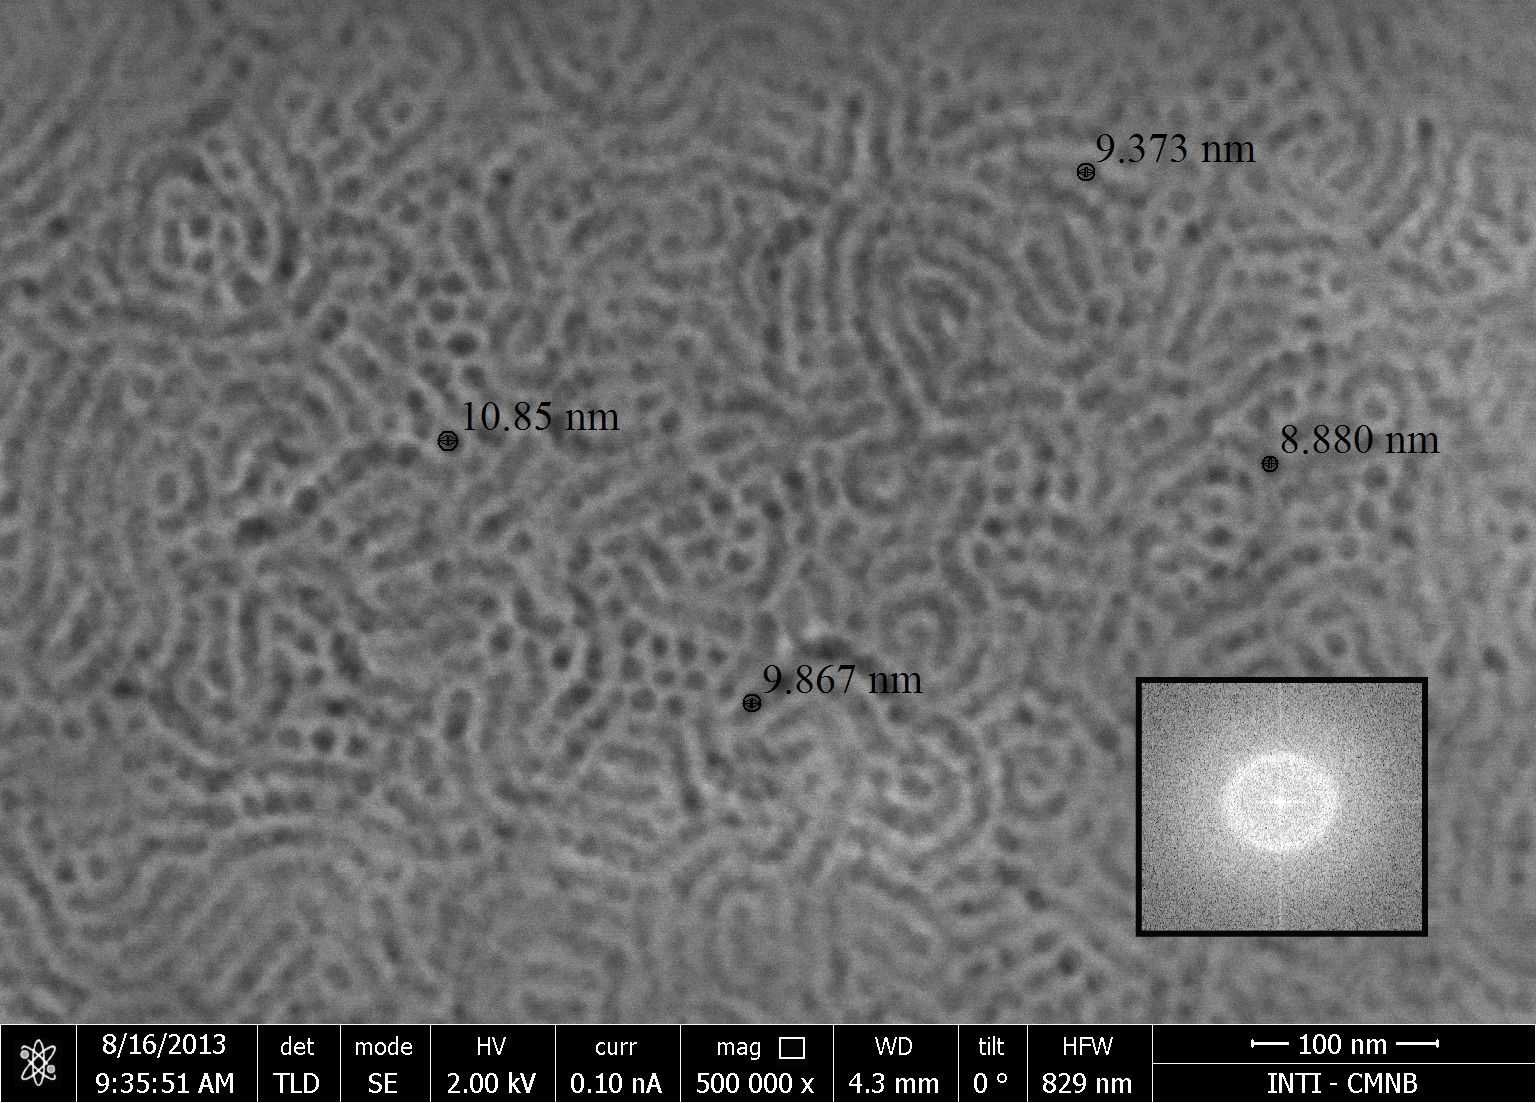
\includegraphics[width=\textwidth]{Imagenes/Superficie-F127-medidas.jpg}
			       		\caption{Microscopía electrónica donde se observa la superficie de una \pdmF\space con poros de \SI{10}{nm} de diámetro en promedio. Recuadro: FFT de la imagen completa.}
			       		\label{fig:sem_homogeneidad1}
			       		\end{subfigure}
			       	\begin{subfigure}[t]{0.495\textwidth}
			 	   	    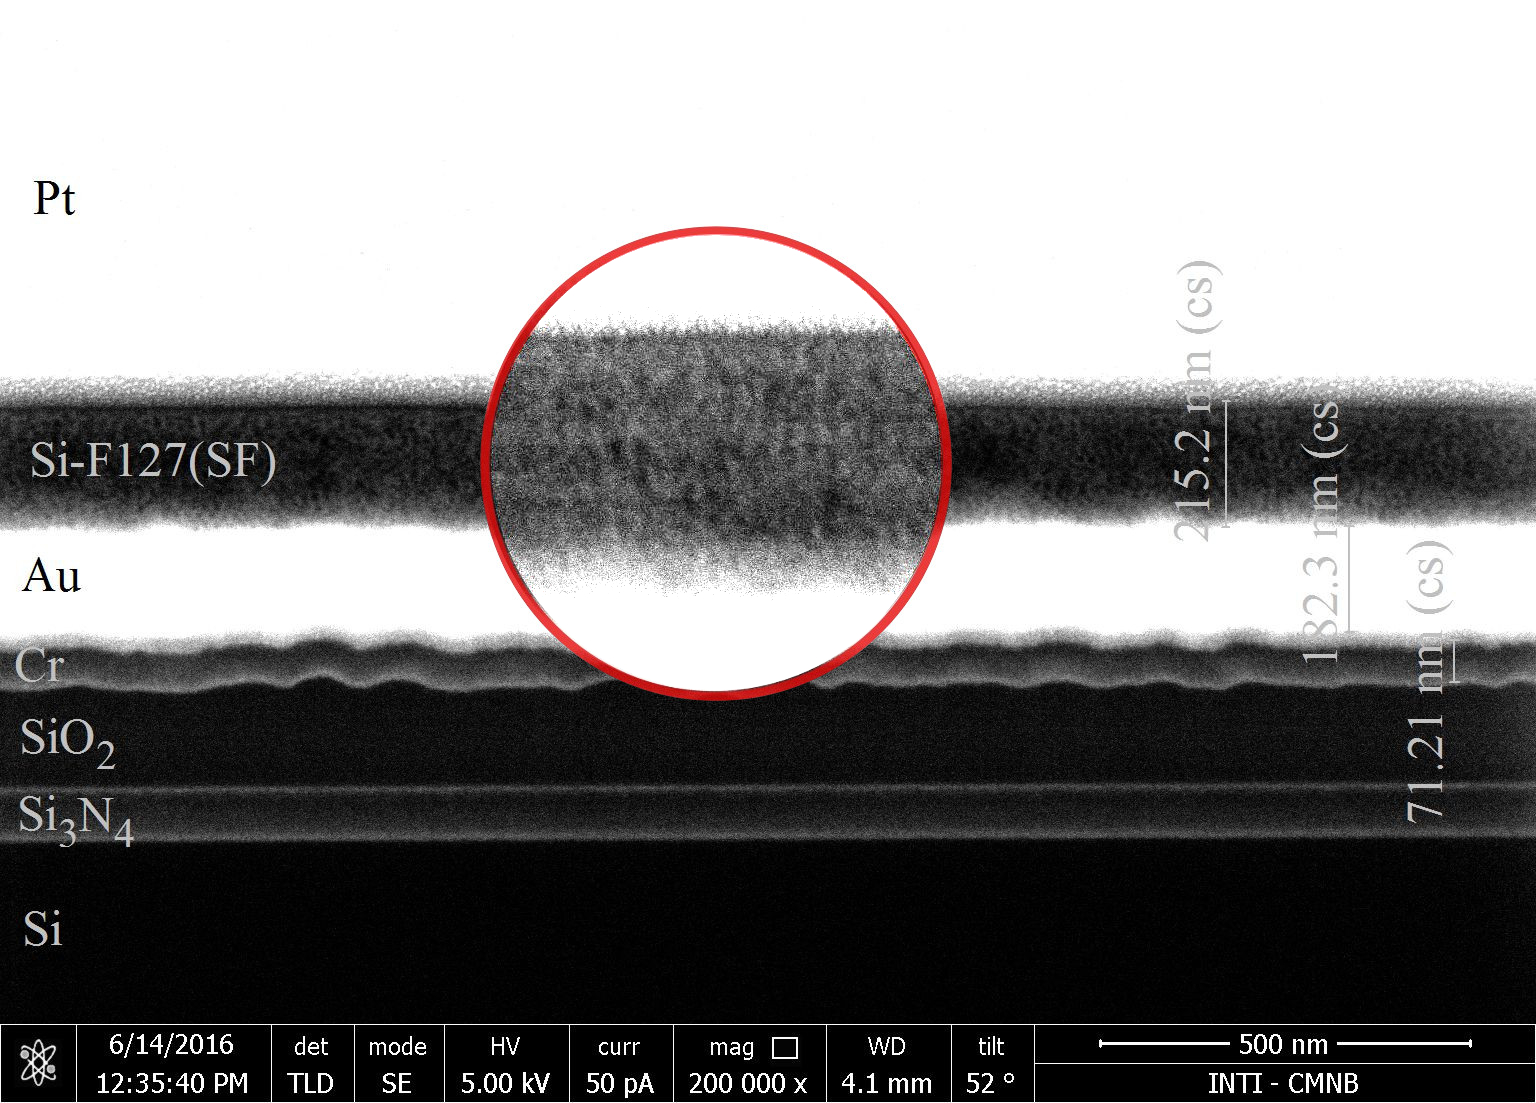
\includegraphics[width=\textwidth]{Imagenes/Perfil-F127.jpg}
			       		\caption{Corte transversal por FIB de una \pdmF\space desde se puede medir el espesor y observar los nanoporos a lo largo del eje transversal de la película.}
			       		\label{fig:sem_homogeneidad2}
			       		\end{subfigure}	
			       	\begin{subfigure}[t]{0.495\textwidth}
			        	\includegraphics[width=\textwidth]{Imagenes/Superficie-CTAB-medidas.jpg}
			       		\caption{Microscopía electrónica donde se observa la superficie regular de muestra \pdmC\space con poros de \SI{3}{nm} de diámetro en promedio.}
			       		\label{fig:sem_homogeneidad3}
			       		\end{subfigure}
					\begin{subfigure}[t]{0.49\textwidth}
			 	   	    \includegraphics[width=\textwidth]{Imagenes/Perfil-CTAB.jpg}
			       		\caption{Corte transversal por FIB de una muestra \pdmC\space en la cual se puede medir el espesor de la película. La resolución transcersal de la técnica no es suficiente para observar los nanoporos.}
			       		\label{fig:sem_homogeneidad4}
			       		\end{subfigure}	
					
					\vspace{-2mm}
					 \caption[MEB \pdmC\space y \pdmF.]{Microscopia para sistemas de sílice porosos con CTAB y F127 calcinados sobre silicio con electrodos de Cr\textbar Au (a y c). Secciones transversales donde se puede apreciar la homogeneidad en el espesor de las películas (b y d).}
					 \label{fig:sem_homogeneidad}	
				     \vspace*{0.2cm}
				     \end{figure}
 	
		 El espesor se controla variando las condiciones de aceleración y velocidad final del \textit{spin-coater}, por lo tanto, para cada condición, se obtiene un espesor diferente. Las rampas de aceleración que se han utilizado para las \pdm\space se muestran en la figura \ref{fig:spin}. Tener control y conocimiento del espesor de las películas es importante para calcular o estimar otras magnitudes, por ejemplo concentración dentro de los poros o la distancia características de difusión. 

		 Algunos autores han desarrollado un marco teórico para establecer la dependencia del espesor con la velocidad de rotación en depósitos de películas poliméricas, encontrando una relación matemática según: \cite{Norrman2005,Meyerhofer1978,Bornside1989,Lora1990}
			\begin{equation}
			  t = k_1 \omega^{\alpha}
			  \label{eq:spin_meso}
			  \end{equation}		
		donde $k_1$ y $\alpha$ son constantes empíricas que dependen de la concentración del monómero, del solvente, del sustrato, de la interacción sol/sustrato y  de las propiedades reológicas del sol. Tal como se mostró en la ecuación \ref{eq:spin_meso}, y siguiendo los reportes de la literatura, el valor de $\alpha$ parece mantenerse contante y en las cercanías de $\alpha=-0.5$ para una gran cantidad de polímeros. 

		Para controlar el espesor de los depósitos se realizaron mediciones del mismo en función de la velocidad final de rotación.  Dichas mediciones fueron tomadas en todos los casos por elipsoporosimetría ambiental (EPA) y sólo en algunos casos selecionados se contrastaron por MEB/FIB, obteniéndose valores comparables por ambas metodologías. Una vez establecido un valor de rotación de referencia se midieron en forma sistemática para cada tratamientos pos-depósito, con ambos surfactantes. Los valores de dichas mediciones se encuentras resumidos en la tabla \ref{tabla:resultados}.
		Los gráficos de la figura \ref{fig:esp} corresponden a la mediciones de espesores en sistemas calcinados. Fueron ajustados matemáticamente por la ecuación \ref{eq:spin_meso} y se obtuvieron valores de $k_1=6413\pm 2300$ y $\alpha=-0.44 \pm 0.04$ para \pdmF\space y $k_1=7601\pm 1800$ y $\alpha=-0.44 \pm 0.04$ para \pdmC. Dichos resultados siguen la tendencia esperada; disminución del espesor con el aumento de la velocidad angular y decaimiento exponencial con $\alpha \approx -0.5$. 

		
			\begin{figure}[!ht]
				\begin{subfigure}[t]{0.495\textwidth}
				\includegraphics[width=\textwidth]{Graficos/Esp_F127.pdf}
				\end{subfigure}
				\begin{subfigure}[t]{0.495\textwidth}
				\includegraphics[width=\textwidth]{Graficos/Esp_CTAB.pdf}
				\end{subfigure}
				\caption[Espesor en función de la velocidad angular]{Control del espesor en función de la velocidad de velocidades angulares para valores comprendidos entre 1000 y \SI{4000}{\minute^{-1}} en sistemas calcinados estructurados con F127 (izquierda) y CTAB (derecha). Todas las mediciones fueron llevadas a cabo por EPA.}
				\label{fig:esp}		
				\end{figure}
	
	\subsection{Adherencia al sustrato de las \pdm}	

		 En numerosos trabajos se ha demostrado la producción de películas delgadas mesoporososas de sílice (con surfactantes como F127, P123, CTAB, Brij56, Brij58, etc.) sobre sustratos de vidrio o silicio. En ninguno de ellos se menciona la existencia de problemas de adherencia al sustrato \cite{Angelome2008,Fuertes2010,Violi2015}. Resulta natural utilizar sustratos de silicio o vidrio debido a la compatibilidad estructural y química que comparten con las películas en base sílice. De hecho tanto película como sustrato son óxidos de silicio. Se conoce que luego de tratamientos térmicos para condensar y calcinar el surfactante, las películas sufren una contracción uniaxial a lo largo del eje normal a la superficie del sustrato debido a la fuerte adherencia al sustrato.\cite{Grosso2004,Soler-Illia2012,Chougnet2005} Uno de los pilares de este trabajo es el depósito de \pdm\space en base silicio sobre sustratos metálicos, más precisamente sobre Au. Sin embargo, se sabe desde hace décadas, que los metales nobles no tienen una buena adherencia sobre sustratos no-metálicos\cite{Kern1990,Hieber1976}, con lo cual es de esperar que también se experimenten problemas de adherencia al querer depositar un sol sobre una película delgada de Au. \cite{Meyer2004,Nugen2009,nasa1973}

		\subsubsection{Adherencia de \pdm\space sobre electrodos de Au}

			En los electrodos en los cuales se depositó \pdm\space estructuradas con Pluronic F127 sobre películas de Au, se observó, en algunos casos, adherencia deficiente. 
			
			Las tres voltametrías cíclicas (VC) de color negro del gráfico \ref{fig:adherencia_F127} corresponden a respuesta de la sonda \aminorutenio (la cual difunde a través de la película) luego de 38 ciclos consecutivos, cantidad de ciclos suficiente para adsorber y saturar la \pdm\space con la sonda. Los mecanismos de transporte, adsorción y forma de las VC (tanto los cambios en la intensidad como los corrimientos en el potencial) se discuten en profundidad en el capitulo \ref{chap:Electroquimica}. La observación de interés para determinar la adherencia es el cambio repentino en dos VC consecutivas (del ciclo 41 al 42). Este cambio sugiere que el sistema muda de la típica respuesta de una sonda que atraviesa una \pdm, a la respuesta habitual de un electrodo desnudo de Au, representado por la voltametría roja. Esta comportamiento sugiere que la película no sufrió una disolución lenta y paulatina, sino que se desprendió del electrodo, total o parcialmente, en algún momento de la medición.
			
				\begin{figure}[th]
				 	   	    \begin{center} 
				        	\includegraphics[width=0.70\textwidth]{Graficos/Adherencia_F127.pdf}
				       		\caption[Adherencia de \pdmF \space sobre una película delgada de Au.]{Serie de voltametrías cíclicas consecutivas, del ciclo 39 al 42, donde se evidencia la falta de adherencia de \pdmF\space sobre electrodo de Au. Las flechas negras indican un cambio repentino en el comportamiento, de un electrodo recubierto con una \pdm\space (negro) a un electrodo desnudo (rojo). Las VC fueron tomadas a \SI{50}{\milli\volt.\second^{-1}} usando de referencia ESC y con sonda \ru\space \SI{1}{\milli\Molar}.}
				         	\label{fig:adherencia_F127}
				     		\end{center}
				     		\end{figure}

			En los casos en los cuales se utilizó CTAB como molde para los poros, el comportamiento es algo diferente. Se manifiestan problemas de adherencia en la mayoría de los tratamientos alternativos, así como en la calcinación. Presentan grietas y fisuras, macro y microscópicas y se observan desprendimientos antes de poder someter los sensores a cualquier medición electroquímica, es decir, apenas terminada la síntesis. Sólo se rescataron algunos pocos casos exitosos de formación de \pdmC\space por calcinación, utilizando como soporte electrodos de Au, y con una superficie lo suficientemente extensa para poder realizar dichas mediciones. Éstos sirvieron para hacer experimentos de EQ conceptuales sobre transporte en poros (consultar capitulo \ref{chap:Electroquimica}), pero en la generalidad de los casos se observa desprendimiento de la película tal como muestran las imágenes de la figura \ref{fig:CTAB_adherencia}.

	     
				\begin{figure}[th]
		 	   	    \begin{subfigure}[t]{0.49\textwidth}
			        	\includegraphics[width=\textwidth]{Imagenes/Au_FCCTAB_adherencia1.jpg}
			       		\end{subfigure}
					\begin{subfigure}[t]{0.49\textwidth}
			 	   	    \includegraphics[width=\textwidth]{Imagenes/Au_FCCTAB_adherencia2.jpg}
			       		\end{subfigure}
					 \caption[Adherencia de CTAB sobre electrodos.]{Microscopías electrónicas donde se muestra la falta de adherencia de \pdmC\space sobre una película delgada de Au. Obsérvese los círculos grises que corresponden, en realidad a burbujas separadas del sustrato. La imagen de la derecha muestra una porción de \pdmC\space despegada y elevada.}
					 \label{fig:CTAB_adherencia}	
				     \end{figure}
			
			Además de la ya mencionada falta de adherencia de los óxidos sobre películas de Au, este desprendimiento se debe, sobre todo, a la interacción CTAB-Au. Es numerosa la información que se encuentra en la literatura sobre la interacción superficial de CTAB sobre películas delgadas y/o nanopartículas de Au. La principal aplicación se basa en la adsorción y autoensamblado del CTAB para controlar el crecimiento y estabilización de nanopartículas de Au. \cite{Cheng2003,Smith2008,Meena2013,Wang2013,Hamon2009} Algunos autores lo utilizan por encima de la concentración micelar crítica (cmc)\cite{Lim2014}o combinado con otros reactivos para favorecer el crecimiento cristalino en alguna dirección preferencial\cite{Smith2009}. Los electrodos de Au, depositados por pulverización catódica, generan películas policristalinas sin favorecer ninguna dirección cristalina.\cite{Svorcik2010,Bechelany2010} Sobre esta superficie las moléculas de CTAB o las micelas se adsorben. Su distribución y densidad a largo de la superficie del electrodo parece depender de la concentración, la orientación cristalina del Au, el solvente y la rugosidad de la superficie\cite{Meena2013,Lim2014}. La adsorción del surfactante en la superficie del electrodo, sumada a la poca adherencia propia del SiO$_2$, son factores que van en demerito de la adherencia y consecuentemente de la formación de \pdmC\space sobre electrodos de Au.
							
		\subsubsection{Estrategias para mejorar la adherencia}\label{sec:adherencia}

			 En función de los resultados expuestos en la sección anterior queda claro que la falta de adherencia de las \pdm\space sobre oro es crítica para la elaboración de los sensores. Por otra parte, al fabricar electrodos de Au con un diseño arbitrario, se suma la dificultad de obtener películas delgadas continuas y adherentes sobre un sistema con dos regiones distintas en su superficie, óxido y metal.
 
             Las estrategias empleadas para promover la adherencia en estos sistemas se basaron en dos conceptos:
				\begin{enumerate}

					\item Optimizar el diseño de forma de minimizar el área metálica de los electrodos, pistas y contactos, ampliando la región del óxido para favorecer la adhenrecia de las \pdm.

					\item Realizar modificaciones superficial en los electrodos, tendiendo puntos de anclaje entre el electrodo y el esqueleto inorgánico de las \pdm.

					\end{enumerate}
			
			 La primera estrategia utilizada para promover una mayor adherencia de las \pdm\space a los sensores, se basa en minimizar el área de contacto electrodo-mesoporoso. Las mayoría de los resultados discutidos en este capítulo fueron realizados en \pdm\space sobre electrodos plenos de Au. Sin embargo, los sensores comprenden un conjunto de electrodos o microelectrodos sobre un sustrato dieléctrico (p. ej. SiO$_2$ o vidrio). Eligiendo un diseño adecuado se puede minimizar el área de los electrodos metálicos. De ésta forma las \pdm\space quedan adheridas fuertemente a los sectores del óxido, donde no está el Au. El resultado final es una película bien adherida sobre una superficie mixta soporte/electrodos.  La figura \ref{fig:adherencia_microelectrodo} representa de manera esquemática esta situación.
			
				\begin{figure}[!ht]
					\begin{center}
					\includegraphics[width=0.80\textwidth]{Esquemas/adherencia_microelectrodo.pdf}
					\caption[Adherencia a los microelectrodos.]{Esquema de un corte transversal de los sensores donde se observan los microelectrodos y la \pdm\space depositada sobre ellos. Las flechas indican las zonas de baja y alta adherencia.}
					\label{fig:adherencia_microelectrodo}
					\end{center}
					\end{figure}
					
					
			 La segunda estrategia se basa en modificar los electrodos mediante una funcionalización superficial, la cual se llevó acabo siguiendo el procedimiento detallado en el capitulo \ref{chap:Materiales}, sección \ref{sec:silanizacion}. Se buscó una molécula compatible con el sistema utilizado, capaz de vincular la superficie del electrodo e integrarse al esqueleto de las \pdm. Se usó para este fin el 3-mercaptopropil trimetoxisilano (MPTMS), el cual es fácilmente de ligar covalentemente al Au por el tiol\cite{Gosser,Byun2013}, y por el otro tiene el silano el cual es perfectamente compatible con el precursor de Si(IV) utilizado\cite{Wu2014,Wu2013,Chen2011}. En la figura \ref{fig:mod_sup} se muestra la molécula en cuestión y un esquema de como queda anclado la \pdm, mediante el MPTMS, al electrodo.
		
			 Una vez realizada la modificación superficial, se llevaron a cabo mediciones EQ para evaluar si los voltagramas sufren distorsiones debido a la funcionalización. Se realizaron dos comparaciones con propósitos diferentes: 1) verificar que la señal sobre un electrodo desnudo no se vea afectada significativamente por la presencia de MPTMS ligado a la superficie del Au; y 2) demostrar que la funcionalización del Au mejora la adherencia cuando se depositan \pdm\space sobre esta superficie modificada.

			 \begin{figure}[!ht]
							\begin{center}
							\includegraphics[width=0.70\textwidth]{Esquemas/mod_sup.pdf}
							\caption[Modificación superficial de los electrodos.]{Izquierda: Molécula de  3-mercaptopropil trimetoxisilano utilizada como ligante entre los electrodos y las \pdm. Derecha: Esquema pictórico de la modificación superficial con MPTMS.}
							\label{fig:mod_sup}
							\end{center}
							\end{figure}
			 \pagebreak
							
			 En la figura \ref{fig:comparaciones_MPTMS-A} se presentan dos voltagramas en los cuales se compara la respuesta para \aminorutenio\space \SI{1}{\milli\Molar} con dos electrodos de Au, uno virgen y otro funcionalizado con MPTMS. Como se puede apreciar en el gráfico la respuesta es prácticamente igual para ambos tipos de electrodos, demostrando que la funcionalización con el tiol no modifica significativamente la respuesta electroquímica.

					\begin{figure}[!ht]
							\begin{center}
							\includegraphics[width=0.70\textwidth]{Graficos/Comparacion_Au-MPTMS.pdf}
							\caption[Comparación de electrodos con y sin MPTMS]{VC para \aminorutenio\space \SI{1}{\milli\Molar} a \SI{50}{\milli\volt\per\second} sobre un electrodo virgen de Au (rojo) comparado con uno funcionalizado con MPTMS (negro). La funcionalización con el tiol no bloquea ni modificar el desempeño electroquímico de los electrodos.}
							\label{fig:comparaciones_MPTMS-A}
							\end{center}
							\end{figure}

             Las voltametrías cíclicas de la figura \ref{fig:comparaciones_MPTMS-B} muestran un típico experimento donde el \aminorutenio\space ingresa y a medida que va difundiendo a lo largo de una película \pdmF, se adsorbe sobre las paredes de la mismas. Dicho voltagrama esta constituido por 30 voltametrías cíclicas consecutivas correspondiente a los ciclos 45 al 75. A partir del ciclo 65 se ve una disminución en la intensidad de pico, la cual es compatible con un fenómeno de disolución de la película y no a un evento de desprendimiento. Los fenómenos de ingreso, adsorción y disolución de las películas se discute en profundidad en el capitulo \ref{chap:Electroquimica}.
       	
					\begin{figure}[!ht]
							\begin{center}
				 	   	    \includegraphics[width=0.70\textwidth]{Graficos/Comparacion_F127-MPTMS.pdf}
				       		\caption[Comparación de superficies con y sin MPTMS.]{Voltametrías cíclicas consecutivas luego de 44 ciclos para \aminorutenio\space \SI{1}{\milli\Molar} realizados a \SI{50}{\milli\volt.\second^{-1}} sobre electrodos modificados con MPTMS. La respuesta es de características similares a la obtenida para este tipo de sistemas, donde se observa el ingreso de la sonda, la adsorción y la disminución de la intensidad debido a un fenómeno de disolución.}
						 \label{fig:comparaciones_MPTMS-B}	
					    \end{center}
					    \end{figure}
			
			 \pagebreak

			 Ambas estrategias para promover la adherencia de las \pdm\space son complementarias y compatibles. Esto quiere decir que se puede optimizar el diseño para minimizar la superficie de electrodos y, a su vez, es posible funcionalizar  con MPTMS las regiones de los electrodos, generando puntos de vinculación entre el mesoporosos y el electrodo. La funcionalización se debe lleva a cabo luego de depositar el Au y antes de realizar el decapado de la fotorresina (consultar sección \ref{sec:fotolito}, pág. \pageref{sec:fotolito}) y no sobre los sensores terminados. De esta forma la modificación queda delimitada sólo a las regiones donde están los electrodos, evitando reacciones colaterales como la silanización del vidrio o silicio con el MPTMS por el extremo del silanol.

			 Es importante resaltar que en los casos que no se utilizó MPTMS, el desprendimiento o despegue de las \pdm\space se hizo evidente por microscopía óptica o durante las mediciones EQ en una fracción de las casos, en otros se observaron grietas, fisuras o discontinuidades en las películas. En contrapartida, en los electrodos que se funcionalizaron con MPTMS, el 100\% de los casos llevaron a la formación de películas continuas, sin grietas y con buena adherencia.

\section{Métodos alternativos de síntesis de \pdm}
	
	 En esta sección se da cuenta de los resultados obtenidos en la fabricación y caracterización de \pdm\space por métodos alternativos a la calcinación. Como ya se mencionó anteriormente, el desarrollo de estos métodos surgió de necesidades que emergieron durante el proceso de fabricación de los sensores. Entre las principales necesidades se cuenta: minimizar la diferencia de expansión térmica entre las películas delgadas mesoporosas y metálicas, evitar procesos difusivos, ampliar sustancialmente la gama de sustratos, mejorar la adherencia y disminuir costos.

	 En este sentido, se idearon metodologías que permiten disminuir la temperatura de procesado hasta \SI{130}{\celsius}, sin perder grado de condensación y manteniendo las características espaciales de los poros. Al no calcinar, se agrega una etapa extra, la eliminación del surfactante. Presentamos a continuación una tabla con la nomenclatura y una breve reseña de los procesos que se exploraron y que fueron descriptos en detalle en la sección \ref{sec:cond_y_extr}.

	 Se exponen primero los resultados de las caracterizaciones de las \pdm\space obtenidas por calcinación. El propósito de ésto es tener datos de referencia para comparar con los métodos alternativos. Luego se discuten los resultados que se obtuvieron por cada uno de ellos y se resumen en la tabla \ref{tabla:resultados}. Finalmente, se expone una discusión global comparando cada una de las técnicas, para cada uno de los métodos. Para facilitar la lectura, la información detallada microscópica y espectroscópica de cada proceso se encuentra en el anexo C.
	 
	  	 \begin{table}[h!] 
		 	 \caption[Tratamientos alternativos de síntesis de \pdm]{Nomenclatura de los métodos alternativos de síntesis de \pdm.}
			 \begin{tabular}{>{\raggedright\arraybackslash}m{1.9cm}>{\centering\arraybackslash}m{1cm}>{\raggedright\arraybackslash}m{0.9cm}>{\raggedright\arraybackslash}m{6.62cm}} 
			 \toprule
				 Método   &  Nomenclatura$^*$&  & Descripción \\ \midrule
				 Calcinado & CalSC CalSF& &  Condensación \SI{130}{\celsius} \SI{1}{hora}\hspace{2cm} Extracción \SI{350}{\celsius} \SI{2}{hora}\hspace{2cm} \\ \midrule
				 Simplificado & SimSC SimSF& &  Condensación \SI{130}{\celsius} \SI{1}{hora}\hspace{2cm} Extracción IpOH / H$_2$O pH=2 \\ \midrule
				 Prolongado & ProSC ProSF& & Condensación \SI{130}{\celsius} \SI{7}{dias}\hspace{2cm} Extracción IpOH / H$_2$O pH=2 \\ \midrule				
				 Vacío & VacSC VacSF VacZSF& &  Condensación \SI{130}{\celsius} \SI{7}{dias}, P=\SI{e-5}{\milli\bar}\hspace{2cm} Extracción IpOH / H$_2$O pH=2 \\ \midrule
				 Ácido & ÁciSC ÁciSF& &  Condensación en atmósfera de HCl\hspace{2cm} Extracción IpOH / H$_2$O pH=2 \\ \midrule
				 Alcalino & AlcSC AlcSF& & Condensación en atmósfera de NH$_3$\hspace{2cm} Extracción IpOH / H$_2$O pH=2 \\ 
				\bottomrule
				   \end{tabular}\vspace*{2pt}
		    	  	\footnotesize{$^*$SC=sílice/CTAB, SF=sílice/F127, ZSF=circonio-sílice/F127}
				   	\label{tabla:tratamientos}
				   \end{table}
	
	 \subsection{Método de calcinación}
	 	
	 		El tratamientos de calcinación luego del depósito del sol es una ruta sintética clásica utilizada por muchos autores para la producción de películas delgadas mesoporosas de óxidos\cite{Soler-Illia2002a,Brinker1999,Soler-Illia2006,Grosso2004,Innocenzi2013,angelome2011}. Consiste en estabilizar las \pdm\space mediante un tratamiento a humedad y temperatura controladas, seguidas de calcinación a \SI{350}{\celsius} para eliminar el molde. Los detalles técnicos se pueden consultar en la sección \ref{sec:cond_y_extr}, pág. \pageref{sec:cond_y_extr}.

	 	  \subsubsection{Análisis de la porosidad}

		 Como veremos en adelante, la porosidad y accesibilidad son factores que determinan la cantidad de analito que se adsorbe o difunde a través de las \pdm, por este motivo resulta fundamental tener herramientas para cuantificar dichas magnitudes. 

		 Del estudio de las películas por MEB se puede obtener información muy valiosa como tamaño y distribución de los poros, así como estudios de la organización espacial de los mismos mediante transformadas de Fourier (FFT). En la figura \ref{fig:F127_Si_Au} se muestran imágenes de MEB para películas \pdmF sobre distintos sustratos, cada una con su respectiva transformadas. De éstas, se hace obtiene que se trata de un arreglo de poros con orden local, con tamaños próximos a los de \SI{10}{\nm} de diámetro, coincidiendo la con información existente en la literatura\cite{urade2005,angelome2011,lee2006} y con los datos obtenidos por EPA (ver más adelante y consultar la tabla \ref{tabla:resultados} para mas información).  

			\begin{figure}[th]
		 	   	    \begin{subfigure}[t]{0.49\textwidth}
			        	\includegraphics[width=\textwidth]{Imagenes/F127_Si_sup.jpg}
			       		\end{subfigure}
					\begin{subfigure}[t]{0.49\textwidth}
			 	   	    \includegraphics[width=\textwidth]{Imagenes/F127_Au_sup.jpg}
			       		\end{subfigure}
					\caption[MEB arreglo poroso para \pdmF\space sobre Si y Au.]{Microscopía electrónica de barrido de sistemas \pdmF\space y sus respectivas FFT. Se observa la distribución y homogeneidad de los poros en superficie. Izquierda: sobre sustrato de silicio. Derecha: sobre sustrato de Au.}	 
					 \label{fig:F127_Si_Au}
					 \end{figure}

		 En el caso de las películas porosas estructuradas con CTAB el análisis por MEB brinda una información más limitada, ya que el diámetro de los poros ($\approx$ \SI{3}{\nm}) esta en el límite de resolución de la técnica para muestras no conductoras. Sin embargo, alcanza para  ver que existe un sistema de poros (ver figura \ref{fig:sem_homogeneidad3}). En este caso, para hacer un estudio por imágenes mas completo, se debería recurrir a microscopía electrónica de transmisión (MET).

		 El estudio por MEB es sumamente útil en muchos aspectos; sin embargo, la información que brinda es de áreas muy pequeñas, superficial y no da información completa sobre la conectividad y cuellos de las películas. Es por ello que se recurrió a la técnica de elipsoporosimetría ambiental (EPA). Ésta es una técnica promedio, donde podemos obtener información valiosa sobre la accesibilidad de agua en los poros, se puede determinar el volumen poroso de las \pdm, la distribución de tamaños de poros y cuellos y la variación del espesor en función de la presión de vapor de agua relativa a la presión de saturación ($\text{P/P}_s$). Para valores crecientes de P/P$_s$, la adsorción en los mesoporos se produce a través de la formación de una monocapa y luego de multicapas de moléculas de agua sobre las paredes de los poros, seguida de condensación capilar, es decir, llenado de los poros con agua líquida. La posterior disminución de la presión externa resulta en la desorción mediante evaporación capilar, vaciando primero el centro de los poros, seguida por la desorción de la multicapa de solvente presente en las paredes de los mismos. Para cada punto de P/P$_s$ en equilibrio se tiene un valor del índice de refracción efectivo ($n$), de esta forma se construye la isoterma de adsorción/desorción de agua. Los cálculos realizados para obtener información estructural (volumen poroso, y distribución de poro y cuello) a partir de las isotermas se basaron en el protocolo detallado los trabajos del grupo de Sánchez y Baklanova\cite{Baklanov2000,Boissiere2005,Sakatani2006}. Los detalles experimentales de esta técnica se presentaron en el capitulo \ref{sec:elipso}, pág. \pageref{sec:elipso}.

		 \pagebreak

		 En las figuras \ref{fig:F127_EPA} y \ref{fig:CTAB_EPA} se presentan las isotermas de adsorción de agua para sistemas calcinados \pdmF\space y \pdmC. Se observa que ambas son de tipo IV, según la clasificación de Brunauer\cite{Gregg1967,Violi2015,Fuertes2010}. Este tipo de isotermas con histéresis entre la rama de adsorción y la de desorción es característico de materiales con mesoporos, donde los poros se llenan por condensación capilar. Por otro lado el ciclo de histéresis se podría clasificar como un ciclo intermedio entre H1 y H2, según la clasificación IUPAC\cite{Thommes2015}. Esto es indicativo de una estructura de poros de tamaño uniforme que formar parte de un red compleja con efectivos significativos sobre la adsorción de solvente.\cite{Thommes2015,Gregg1967,Lowell2004,Sing1985}

		 En las figuras \ref{fig:F127_PSD} y \ref{fig:CTAB_PSD} se muestran se muestran las distribuciones de tamaño de poro para estos sistemas. Dichas distribuciones se obtuvieron a partir de las isotermas, y se extrajo información estructural tanto de la rama de adsorción como de la de desorción.


		     	  	\begin{figure}[!ht]
		     	  		\begin{subfigure}[t]{0.495\textwidth}
		     	  		\includegraphics[width=\textwidth]{Graficos/SI_F127_Calcinado_EPA.pdf}
						\caption{Elipsoporosimetría de una \pdmF\space depositada sobre silicio sintetizada por calcinación.}
						\label{fig:F127_EPA}
						\end{subfigure}
						\begin{subfigure}[t]{0.495\textwidth}
		     	  		\includegraphics[width=\textwidth]{Graficos/SI_F127_Calcinado_PSD.pdf}
						\caption{Distribución de tamaño de poro y cuello correspondientes a la isoterma de (a).}
						\label{fig:F127_PSD}
						\end{subfigure}
						\caption[Elipsoporosimetría para sistemas \pdmF.]{(a) Curva de adsorción/desorción de agua para una \pdmF\space. La misma corresponde a una isoterma de tipo IV con un lazo de histéresis de tipo H1/H2, lo cual se concuerda con materiales mesoporosos con poros y cuellos interconectados. (b) Distribución de poros y cuellos con tamaño de poros uniformes, de aproximadamente \SI{10}{\nm} de diámetro.}
						\end{figure}
					\begin{figure}[!ht]
		     	  		\begin{subfigure}[t]{0.495\textwidth}
		     	  		\includegraphics[width=\textwidth]{Graficos/SI_CTAB_Calcinado_EPA.pdf}
						\caption{Elipsoporosimetría de una \pdmF\space sobre sustrato de silicio sintetizada por el método clásico de calcinación.}
						\label{fig:CTAB_EPA}
						\end{subfigure}
						\begin{subfigure}[t]{0.495\textwidth}
		     	  		\includegraphics[width=\textwidth]{Graficos/SI_CTAB_Calcinado_PSD.pdf}
						\caption{Distribución de tamaño de poro y cuello correspondientes a la isoterma de (a).}
						\label{fig:CTAB_PSD}
						\end{subfigure}
						\caption[Elipsoporosimetría para sistemas \pdmC.]{(a) Curva de adsorción/desorción de agua para una \pdmC\space . La misma corresponde a una isoterma de tipo IV con un lazo de histéresis de tipo H1/H2, lo cual se concuerda con materiales mesoporosos con poros y cuellos interconectados. (b) Distribución de poros y cuellos con tamaño de poros uniformes, de aproximadamente \SI{3}{\nm} de diámetro.}
						\end{figure}	
		
		 	\pagebreak

		 	Del conjunto de resultados presentados cabe resaltar que son películas homogéneas, sin grietas ni discontinuidades tanto a nivel macro como microscópico, con poros organizados localmente y distribución de tamaños de poros y cuellos estrecha . Las \pdm\space estructuradas con F127 presentan poros y cuellos de 9 y \SI{4.5}{\nm} de diámetro respectivamente, mientras que las estructuradas con CTAB, 2.5 y \SI{2}{\nm}. También se pueden extraer los valores de $n$, porcentaje de volumen poroso (\%V) y espesor los cuales se resumen en la tabla \ref{tabla:resultados}. Estos valores son los que se usarán para establecer un parámetros de condensación y porosidad de las \pdm\space y se usaran como semilla para la discusión comparativa con los resultados obtenidos para el resto de los tratamientos.

	      \subsubsection{Análisis por FTIR}\label{sec:Analisis_IR}

		 Son muchos los trabajos en los cuales se caracterizan las películas delgadas de SiO$_2$ por IR\cite{Olsen1989,Almeida1990,Redol1997,Innocenzi2003}, y también muchos otros que recolectan y emplean dichos resultados.\cite{Angelome2008,Calvo2008,Calvo20210}.
		 El análisis de espectroscopia infrarroja por transformada de Fourier (FTIR) se utilizó en esta tesis para identificar y caracterizar la estructura inorgánica porosa de SiO$_2$, evaluar comparativamente la condensación del óxido, y determinar la presencia de grupos orgánicos, en particular residuos de surfactante. 

		 Innocenzi ha realizado un análisis completo y bien fundamentado sobre las vibraciones en el IR, de películas delgadas de SiO$_2$ tanto densas como mesoporososas.\cite{Innocenzi2003} Para los enlaces Si-O-Si, se observa la presencia de 4 modos de vibración óptico-trasversales (TO$_x$) y 4 modos óptico-longitudinales (LO$_x$) en películas delgadas de SiO$_2$. Aquellas películas de SiO$_2$ sintetizadas por sol-gel se caracterizan principalmente por presentar tres de los cuatro modos transversales, los cuales en general son tomados como huella digital para este tipo de materiales.\cite{Innocenzi2003,Angelome2008,Calvo2008} El modo TO$_1$, presenta una banda débil $\approx$\SI{460}{\cm^{-1}} asociada a movimientos de balanceo; el modo TO$_2$ está asociado a un estiramiento simétrico con un pico débil cercano a $\approx$\SI{800}{\cm^{-1}}; el modo TO$_3$ presenta un pico intenso centrado en $\approx$\SI{1075}{\cm^{-1}} y se asocia a vibraciones asimétricas del enlace Si-O-Si. 

		 		 \begin{figure}[!ht]
						\begin{center}
						\includegraphics[width=0.90\textwidth]{Imagenes/modos-infra.jpg}
						\caption[Modos de vibración Si-O-Si]{Representación de los movimientos de vibración del oxigeno (gris oscuro) respecto de los átomos de silicio (gris claro).(a) y (b) estiramientos simétrico perpendicular a plano Si-Si. (c) y (d) estiramientos antisimétrico paralelo a la recta Si-Si. (e) y (f) balanceo perpendicular al plano Si-O-Si. La figura fue adaptada de la publicación \textit{Infrared spectrocopy of sol-gel derived silica-based films: a spectra-microstructure overvire}, J. Non. Cryst. Solids, 316(2-3), p. 309-319. }
						\label{fig:modos-ir}
						\end{center}
						\end{figure}

		 El modo TO$_4$ por lo general no es observable, algunos autores lo reportan como una banda muy débil en las cercanías de \SI{1150}{\cm^{-1}} \cite{Pai1986,Grosse1986}. La figura \ref{fig:modos-ir} es una representación esquemática de los tres principales modos de vibración: TO$_1$, TO$_2$ y TO$_3$.

		 En experimentos de incidencia normal a la superficie, solo deberían excitarse las vibraciones óptico-transversales, sin embargo se observan banda de vibraciones correspondientes a modos óptico-longitudinales asociadas a oscilaciones colectivas acopladas TO-LO\cite{Pai1986,Grosse1986,Innocenzi2003}. Los modos ópticos-longitudinales, LO$_1$ y LO$_2$ no son visibles, y LO$_3$, aparece como un hombro de la banda TO$_3$ a mayores frecuencias. La observación experimental de LO$_4$ es escasa, cuando se observa aparece como una banda muy débiles en la zona comprendida entre 1200 y \SI{1150}{\cm^{-1}} \cite{Pai1986,Grosse1986}.
				 
				 \begin{figure}[!b]
						\begin{center}
						\includegraphics[width=0.83\textwidth]{Graficos/IR_Denso.pdf}
						\caption[FTIR SiO$_2$ denso y SiO$_2$ mesoporoso.]{Espectro de absorción de IR de una película SiO$_2$ denso depositada por \textit{sputtering }comparada con una de SiO$_2$ mesoporoso. Se observa, para las \pdm, la aparición de un marcado hombro en \SI{1180}{\per\cm} debido al acoplamiento TO$_3$-LO$_3$ y un pico correspondiente a la vibración $\nu$Si-OH.}\index{sputtering@\textit{sputtering}}
						\label{fig:IR-denso}
						\end{center}
						\end{figure}

		 Otra observación relevante, realizadas por Almeida y Pantano\cite{Almeida1990}, es la naturaleza del hombro presente en $\approx$\SI{1180}{\cm^{-1}}, el cual se intensifica con el aumento de la porosidad de la película y lo asocia a un acoplamiento de los modos LO$_3$ y TO$_3$ con predominancia de carácter LO. Este fenómeno parece estar asociado a la dispersión de la radiación IR dentro de los poros y la consecuente activación del modo longitudinal.	
			
		 Se pudo corroborar dicha observación en los espectros de la figura \ref{fig:IR-denso}, donde se compara una \pdm\space con una película delgada de SiO$_2$ depositada por \textit{sputtering}.  Allí se ve el hombro bien acentuado para la \pdm\space y una banda en $\approx$\SI{965}{\cm^{-1}} asociada al estiramiento Si-OH/Si-O$^-$; mientras que para la película de SiO$_2$ denso depositada por \textit{sputtering} ($n\sim 1.5$ a $\lambda=$\SI{600}{\nm})\cite{Vergohl1999} se observa la ausencia del hombro, aparición de la incipiente banda de LO$_4$ y desaparece la banda del Si-OH/Si-O$^-$.

		 Además del análisis de la estructura inorgánica, se utilizó FTIR para evidenciar la presencia del surfactante usado de molde para los poros. Se centrará la atención en las bandas que corresponden a las vibraciones del enlace C-H, las cuales aparecen en la zona de 2950 a \SI{2850}{\cm^{-1}}. En la figuras \ref{fig:IR_F127_calciando} y \ref{fig:IR_CTAB_calcinado} se comparan \pdm\space calcinadas \SI{350}{\celsius} y sin calcinar para los surfactantes utilizados. Se ve como desaparecen las bandas correspondientes a al vibración C-H debido a la eliminación del surfactante. Se conserva la forma del hombro a $\approx$\SI{1180}{\cm^{-1}} indicador de una estructura porosa y se observa la banda en en $\approx$\SI{965}{\cm^{-1}} asociada al estiramiento Si-OH/Si-O$^-$, el cual según algunos autores sólo desaparece cuando las películas son sometidas a T$>$\SI{500}{\celsius} debido a la condensación de grupos silanol en la superficie.\cite{Innocenzi2003,Almeida1990,Bertoluzza1982}

				\begin{figure}[!h]
						\begin{center}
						\includegraphics[width=0.83\textwidth]{Graficos/IR_F127.pdf}
						\caption[FTIR para una \pdmF.]{Espectro de absorción para una \pdmF\space antes y después de calcinar, donde se puede apreciar la aparición de un pico fuerte el cual correspondiente al surfactante F127.}
						\label{fig:IR_F127_calciando}
						\end{center}
						\end{figure}
				
				\begin{figure}[!hb]
						\begin{center}
						\includegraphics[width=0.83\textwidth]{Graficos/IR_CTAB.pdf}
						\caption[FTIR para una \pdmC.]{Espectro de absorción para una \pdmC\space antes y después de calcinar, donde se puede apreciar la aparición de un pico fuerte el cual correspondiente al surfactante CTAB.}
						\label{fig:IR_CTAB_calcinado}
						\end{center}
						\end{figure}		
		 
		  Estos espectros IR, obtenidos para películas calcinadas, se utilizarán de referencia para comparar con los espectros IR de \pdm\space producidas por métodos alternativos a la calcinación. Por un lado, se evalúa la presencia de poros, indicado por la presencia del hombro LO$_3$-TO$_3$ y  por otro, el grado de condensación, siguiendo la relación de picos Si-O-Si/Si-OH. Por último, la técnica es utilizada para corroborar la eliminación del surfactante por ausencia de la banda $\approx$\SI{2900}{\per\cm} correspondiente a la vibración C-H.

		 En la tabla que sigue, se asignan las vibraciones observadas que servirán de referencia para el análisis de resultados de las próximas secciones.

		 	\begin{table}[ht!] 
		 	 \caption[Asignación de vibraciones en el IR]{Bandas y asignación de vibraciones en el IR frecuentemente observadas a lo largo de la tesis.}
			 \begin{tabular}{>{\raggedright\arraybackslash}m{2.6cm}>{\centering\arraybackslash}m{2.55cm}>{\raggedright\arraybackslash}m{5.7cm}} 
			 \toprule
				 Posición (\si{\per\cm})   &  Vibración &  Presente en \\ \midrule
				 3500-3000	& $\nu_\text{OH}$ & H$_2$O, 2-propanol \\ \midrule
				 2950-2850  & $\nu_\text{C-H}$ & Molde (CTAB, Pluronic F127) \\ \midrule
				 2450		& CO$_2$ & CO$_2$ ambiental \\ \midrule
				 2000-1200  & H$_2$O & Estructura fina del H$_2$O\hspace{2cm} H$_2$O adsorbida  \\ \midrule
				 1250		& $\nu_\text{Si-O-Si}$ & SiO$_2$ denso LO$_3$ \\ \midrule
				 1170		& $\nu_\text{Si-O-Si}$ & SiO$_2$ denso LO$_4$ \\ \midrule
				 1075		& $\nu_\text{Si-O-Si}$ & SiO$_2$ TO$_3$ \\ \midrule
				 1180 (hombro) & $\nu_\text{Si-O-Si}$ & SiO$_2$ poroso acoplamieno LO$_3$-TO$_3$ \\ \midrule
				 965 		& $\nu_\text{Si-OH}$ & SiO$_2$ parcialmente condensado silanoles superficiales\\ \midrule 
				 800		& $\nu_\text{Si-O-Si}$ & SiO$_2$ denso TO$_2$ \\
				 \bottomrule
				   \end{tabular}
				   	\label{tabla:ftir}
				   \end{table}

	      \subsubsection{Accesibilidad de las PDM}\label{sec:acc}

			Hasta ahora se han evaluado muchos de los aspectos fundamentales para poder pensar en utilizar las películas mesoporosas de óxido de silicio como componentes de sensores: estructura porosa, volumen poroso, compatibilidad de sustratos, técnicas de depósito, control del espesor, etc. 

			Sin embargo, se debe considerar un aspecto crítico para utilizar estas películas como parte de un sensor electroquímico. Se debe garantizar el libre acceso de los analitos a través de los nanoporos, de forma de poder difundir hasta la superficie del electrodo, para que tenga lugar allí, la reacción electroquímica.

			Para evaluar el transporte de especies a través de los materiales, se coloca una solución con una sonda electroquímica adecuada, en la celda de medición en contacto con el electrodo. La forma en que fueron tomadas las medidas se explica extensamente en la sección \ref{sec:medidas_eq}, pág \ref{sec:medidas_eq}. 

			La figura \ref{fig:accesibilidad} muestra dos voltametrías cíclicas, una para \pdmF\space y otra para \pdmC\space en presencia de \aminorutenio\space \SI{1}{\milli\Molar} en solución de KCl \SI{0.1}{\Molar}. En ambos voltagramas se registra una respuesta electroquímica, demostrando que la superficie del electrodo se encuentra accesible. Los resultados sugieren que existe un camino percolativo en las \pdm, tanto si se estructuran con F127 o con CTAB, que permite, o bien que la señal electroquímica se propague desde el seno de la solución hasta el electrodo (transporte de carga) o bien que el analito difunda desde la solución al electrodo (transporte de masa). Los diferentes mecanismos de trasporte involucrados en estos experimentos, son tema central de esta tesis y se discuten en detalle en el capitulo \ref{chap:Electroquimica}. De estos experimentos preliminares se puede concluir que la síntesis de \pdm\space sobre electrodos lleva a películas que, al menos en parte, son accesibles y permiten a una sonda EQ difundir hasta la superficie del electrodo.   

						\begin{figure}[th]
				 	   	    \begin{subfigure}[t]{0.495\textwidth}
				        	\includegraphics[width=\textwidth]{Graficos/SF-accesibilidad.pdf}
				       		\caption{Voltametría Cíclica sobre \pdmF}
				         	\end{subfigure}
				         	\begin{subfigure}[t]{0.495\textwidth}
				        	\includegraphics[width=\textwidth]{Graficos/SC-accesibilidad.pdf}
				       		\caption{Voltametría Cíclica sobre \pdmC}
				         	\end{subfigure}
				     		\caption[Accesibilidad electrodo de trabajo.]{Voltametrías Cíclicas de \aminorutenio\space \SI{1}{\milli\Molar} sobre Au recubierto con \pdm\space con una velocidad de barrido \SI{50}{\milli\volt\per\second} utilizando como referencia ESC.}
				     		\label{fig:accesibilidad}
				     		\end{figure}
	
	 \subsection{Método simplificado}

		 	De todos los tratamientos pos-depósito, se denomina método simplifcado a aquel que sigue los procedimientos establecidos en la literatura para eliminar el surfactante sin recurrir a la calcinación.\cite{Angelome2008,Calvo20210,Calvo2010,Fuertes2009} El proceso consiste en estabilizar las \pdm\space a \SI{130}{\celsius} durante \SI{1}{\hour} y luego extraer el surfactante en reflujo de 2-propanol durante \SI{15}{\minute}. 
			
			En el análisis por microscopía se aprecia que las \pdmF\space sometidas a éste tratamiento se adhieren correctamente en ambos sustratos, quedan bien estructuradas, sin grietas ni discontinuidades y se obtienen poros uniformes en tamaño y con estructuras de orden local (figura \ref{fig:Microscopia_F127_simplificado}). Las \pdmC\space sobre silicio también adhieren bien y no presentan grietas, mientras que sobre Au presentan grietas y discontinuidades en su estructura (figura \ref{fig:Microscopia_CTAB_simplificado}), lo cual se adjudica al hecho de la adsorción del bromuro sobre el Au, tema que ya fue discutido en la sección \ref{sec:adherencia}, pág. \pageref{sec:adherencia}. 
			
			La caracterización por elipsoporosimetría para las \pdmF\space resultó en una isoterma tipo IV con histéresis H5 para las \pdmC\space y tipo IV con histéresis H2 para las \pdmF\cite{Thommes2015}. Los sistemas estructurados con CTAB presentan una porosidad del 40\% aproximadamente, con una histéresis pequeña entre las ramas de adsorción y desorción de la isoterma. Esto posiblemente signifique, que no hay prácticamente diferencia entre el tamaño de poro y cuello (figuras \ref{fig:CTAB_simplificado_EPA}  y \ref{fig:CTAB_simplificado_PSD}). Este diámetro de poro pequeño se puede atribuir a que el surfactante ha sido sólo parcialmente eliminado de la estructura, estrechando el tamaño de poro hasta hacerlo prácticamente igual tamaño de los cuellos.
			En el caso de los sistemas \pdmF\space la adsorción de agua se produce en una única etapa mientras que la desorción ocurre a dos valores de presión diferentes, a P/P$_s=0,65$ y a P/P$_s=0,45$ (figura \ref{fig:F127_simplificado_EPA_2}). 

			Thielemann \cite{Thielemann2011} y Groen\cite{Groen2003} proponen que este comportamiento se produce al desorber el agua ocluida en poros, que están más o menos <<bloqueados>> por el diámetro de los cuellos, tal como se ejemplefica en la figura \ref{fig:thielemann}. Al producirse la desorción del agua a través de cuellos de distinto tamaño, la fuerza  necesaria para vencer la tensión superficial debe ser mayor, desorbiendo a menor P/P$_s$ cuanto menor sea el diámetro de los cuellos; tal como predice la ecuación de Kelvin (ver ecuación {\ref{eq:kelvin}). Esta observación se repite para varios de los tratamientos practicados e indica una población de cuellos con una doble distribución de tamaño (figura \ref{fig:F127_simplificado_PSD}). Esto sugiere dos posibilidades: 1) la existencia de dos sistemas porosos no conectados entre sí, o 2) falta de condensación en el sistema porosos con cuellos o poros medianamente ocluidos por sílice parcialmente condensada.

			%Grafico de Thielemann
			\begin{figure}[th]
		 	   	    \begin{subfigure}[t]{0.49\textwidth}
			       	\includegraphics[width=0.90\textwidth]{Graficos/Doble-distr.png}
			       	\caption{Efecto de poros bloqueados en silice calcinada estructurada con Pluronic 123.}
			       	\label{fig:thielemann}
			   		\end{subfigure}
			   		\begin{subfigure}[t]{0.49\textwidth}
			   	    \includegraphics[width=\textwidth]{Graficos/SI_F127_simplificado_EPA.pdf}
			   	    \caption{Isoterma de adsorción/desorción de agua realizada por EPA para una \pdmF.}
			   		\end{subfigure}
					 \caption[Microscopías \pdmF\space tratamiento simplificado.]{Isotermas obtenidas para sílice mesoporosa con poros bloquedados. (a) Isoterma extradida de la publicación de Thielemann\cite{Thielemann2011} y, (b) isoterma para sistemas \pdmF\space condensadas y extraídas por el métodos simplificado.}
					 \label{fig:F127_simplificado_EPA_2}	
				     \end{figure}

			 En los espectros de IR, para ambos sistemas de poros (figuras \ref{fig:IR_CTAB_simplificado} y \ref{fig:IR_F127_simplificado}), se observa, entre otras, el típico acoplamiento TO$_3$-LO$_3$ que resultan en un hombro a \SI{1180}{\cm^{-1}}} indicativo de una estructura porosa\cite{Innocenzi2003}. También se ha estimado el grado de condensación en función de la relación en la intensidad de las bandas para $\nu_{\text{Si-O-Si/}}\nu_{\text{Si-OH}}$ y el porcentaje de extracción del surfactante siguiendo la intensidad de la banda para el estiramiento C-H. Como se discutirá más adelante, ésta vibración puede no sólo estar asociada al surfactante sino a la esterificación de grupos etóxidos con silanoles superficiales durante el proceso de extracción alcohólica.

			 Todos los resultados, para este y todos los tratamientos, se encuentran resumidos en la tabla \ref{tabla:resultados}.

	 \subsection{Método prolongado}

	 	 Este tratamiento se basó en prolongar el tiempo de condensación. Luego de la estabilizar las \pdm\space en cámara de humedad ($t=$\SI{1}{\hour}50 \% HR) se colocó en horno a \SI{130}{\celsius} por el término de 7 días, luego se llevó a cabo la extracción del surfactante. La elección de un período de 7 días se debe a que experimentos realizados por 1,2 y 5 días resultaban en sistemas porosos poco estables. Luego, con el propósito de estandarizar y sistematizar los experimentos y procesos de este trabajo se utilizó esté período como tiempo estándar de condensasción.

	 	 Los resultados de este proceso llevaron a depósitos homogéneas sobre silicio, sin discontinuidades ni grietas y con poros bien formados para ambos surfactantes. Cuando se utilizó Au como sustrato, sólo se obtuvieron películas de buen aspecto cuando se las estructuró con F127. Para las estructuradas con CTAB se observaron grietas y sectores enteros completamente desprendidos de los electrodos. Nuevamente, al igual que en el tratamientos anterior, este hecho sugiere que la adsorción de las micelas de CTAB al oro impiden la adhesión de las \pdmC\space a los electrodos (figuras \ref{fig:Microscopia_F127_prolongado} y \ref{fig:Microscopia_CTAB_prolongado}).

	 	 Respecto de la caracterización por EPA, para \pdmF, se observa la misma distribución de <<doble cuello>> o poros bloqueados que en el caso del tratamiento simplificado (figura \ref{fig:F127_prolongado_EPA}). En cambio, los sistemas \pdmC\space sometidos a este tratamiento muestran isotermas prácticamente idénticas al sistema calcinado, con poros de \SI{2,5}{\nm} y cuellos de \SI{1,9}{\nm} (figura \ref{fig:CTAB_prolongado_EPA}).

	 	 Los gráficos de espectroscopia IR para ambos sistemas de poros, F127 y CTAB (figuras \ref{fig:IR_F127_prolongado} y \ref{fig:IR_CTAB_prolongado}), muestran que la extracción fue exitosa. Si bien en el caso de las \pdmC\space se ve todavía una pequeña cantidad de surfactante, la cantidad relativa al no extraído es mucho menor que en el tratamiento simplificado, indicando que la extracción fue mayor. La condensación también se ha mejorado, respecto del tratamiento anterior, tal como indica el aumento relativo de la vibración correspondiente al estiramiento Si-O-Si, lo cual sugiere una maduración de la estructura porosa debido a la elongación en el tiempo de condensación. Los valores porcentuales de ambas observaciones se pueden consultar en la tabla \ref{tabla:resultados}.

	 \subsection{Método de alto vacío}\label{sec:trat-vacio}

	     Luego del éxito parcial del tratamiento prolongado, donde se obtuvieron películas homogéneas y con arreglos de poros bien formados y con estructuras comparables a la de las películas mesoporosas calcinadas\cite{Mogilnikov2002,Fuertes2008,Rothen1945}, se realizó un tratamiento similar, en cuanto a duración y temperatura (7 días a \SI{130}{\celsius}), pero colocando las muestras en alto vacío, a \SI{e-5}{\milli\bar}.

		 El motivo de llevar a cabo este tratamiento fue abastecer al sistema de calor, durante un período tiempo, para darle oportunidad de relajar y estabilizar el cristal líquido y, a la vez, aplicando vacío, desplazar el equilibrio de la reacción  \ref{eq:vacio} según el principio de Le Chatelier\cite{Atkins2006}, removiendo productos de reacción volátiles (H$_2$O y alcoholes) y así favorecer la condensación del óxido.\cite{Zhuravlev2000}

	 		\begin{equation}
				 \schemestart 
				 Si-OH + X-O-Si 
				 \arrow{->[\scriptsize{T=\SI{130}{\celsius},P=\SI{e-5}{\milli\bar}}][\scriptsize{X=H,CH$_3$CH$_2$}]}[0,2.5] 
				 Si-O-Si + X-OH $\hspace{-0.1cm}\Big\uparrow$
				 \schemestop
				 \label{eq:vacio}
				 \end{equation}
				
		 Para sistemas \pdmF, las microscopías ópticas muestran películas homogéneas, sin discontinuidades ni grietas mientras que las imgagenes de MEB revelan la presencia de nanoporos sobre ambos sustratos, silicio y oro, con poros de \SI{9}{\nm} de diámetro (ver figura \ref{fig:Microscopia_F127_vacio}). Respecto de las películas estructuradas con CTAB, presenta el mismo comportamiento que en los casos anteriores: se observa un depósito homogéneo y sin grietas cuando se depositan sobre silicio, pero se observan discontinuidades y grietas cuando se depositan sobre Au \ref{fig:Microscopia_CTAB_vacio}.

		 La isoterma de adsorción/desorción de H$_2$O muestra que desaparece la doble distribución de cuellos que se observó en los tratamientos anteriores para las películas estructuras con F127 (figuras \ref{fig:F127_vacio_EPA} y \ref{fig:F127_vacio_PSD}). El resultado es una isoterma tipo IV con histéresis H2, propia de sistemas con poros monodispersos uniformemente distribuidos, alcanzando un índice de refracción de $n=1,25$ (a P/P$_s$=0\%) y una porosidad de $38\%$, valores próximos a los de un sistema calcinado. A su vez, para \pdmC, el resultado por PEA es una isoterma que devuelve una porosidad (44 \%) y un índice de refracción ($n=1,393$) prácticamente igual al del calcinado (figura \ref{fig:CTAB_vacio_EPA}) con una distribución de tamaño de poros y cuellos (figura \ref{fig:CTAB_vacio_PSD}) comparable con la reportada por Boissiere\cite{Boissiere2005}.

		 De los espectros IR  (figuras \ref{fig:IR_F127_vacio} y \ref{fig:IR_CTAB_vacio}) se puede concluir que que la extracción del surfactante (ya sea para las películas estructuradas con F127 o estructuradas con CTAB) fue buena, pero no total, obteniendo valores de extracción por encima del 85\%. Para ambos sistemas la relación de intensidades $\nu{\text{Si-O-Si/}}\nu{\text{Si-OH}}$, así como un ángulo de contacto alto, demuestran que se trata de una estructura porosa con pared bien condensada. Los valores se encuentran en la tabla \ref{tabla:resultados}.

		 %Fijarse de algun trabajo de mesosporoso con angulo de contacto para poner de referencia.

	 \subsection{Método ácido}

	 	 Algunos autores proponen que un medio fuertemente ácido (pH$<1$) favorece la hidrólisis del alcóxido y la condensación de los grupo siloxano \cite{Soler-Illia2011,Doshi2000a,Huo1996,Boissiere2000,Beck1992}. Las películas depositadas, estabilizadas en cámara de humedad y  parcialmente condensadas a \SI{130}{\celsius}, tal como se explica en la sección \ref{sec:cond_y_extr}, pág. \pageref{sec:cond_y_extr}, fueron expuestas a una atmósfera de HCl durante \SI{15}{\minute}. 

		 En las microscopias para las \pdm\space sometidas a este método (ya sean estructuradas con F127 como con CTAB) se observan grietas y discontinuidades cuando se depositaron sobre electrodos de Au (figuras \ref{fig:Microscopia_F127_acido} y \ref{fig:Microscopia_CTAB_acido}). Este hecho se ha atribuido a una condensación rápida, catalizada por el medio extremadamente ácido. Al no presentar buena adherencia sobre el sustrato, las películas de sílice se contraen en todas las direcciones, y no solo en la dirección normal a la superficie, como ocurre en las \pdm\space depositadas sobre silicio, donde las fuerzas de adherencia al sustrato priman por sobre las fuerzas contracción en el plano\cite{Sakatani2006,Boissiere2005,Guillemin2010}. En ese caso las películas quedan bien formadas y homogéneas en toda el área de la muestra para ambos surfactantes. Se ha observado por microscopía electrónica que para los sistemas \pdmF\space (\ref{fig:Microscopia_F127_acido}) los  poros están casi unidos formando una especie de poro elongado, propio de una estructura \textit{p6mm}\cite{GonzalezSolveyra2017}. 
	
		 Esta morfología superficial de poros elongados se corroboró por PEA (figura \ref{fig:F127_acido_EPA}). Allí se observa, en la isoterma de adsorción/desorción de agua, una doble distribución de cuellos donde predominan cuellos de diámetro grandes, casi del mismo tamaño que los poros, coincidiendo con la observación por microscopía electrónica.
		 Como se puede apreciar en la tabla \ref{tabla:resultados}, las dimensiones de los poros, medidos por por ambas técnicas, dan valores diferentes. Esta discrepancia posiblemente se deba a que la medición por PEA no resulte del todo apropiada para este tipo de estructuras de poros elongados, no esféricos, suposición necesaria para el calculo de las dimensiones de los poros. En cambio, mediante MEB se puede extrapolar la curvatura para simular una esfera y medir los poros, obteniéndose valores de diámetro similares a los de las \pdmF sintetizadas por otros métodos.

		 La isoterma de adsorción/desorción de agua para \pdmC\space muestra que se trata de sistemas con una porosidad del 38\% y un índice de refracción $n=1.23$, al igual que en el caso del F127 apenas superior que en el caso de lo sistemas calcinados.
		
		 En lo referente a la etapa de extracción, se observa por espectroscopia IR, que fue efectiva para ambos sistemas de poros, alcanzando un alto porcentaje de extracción, $91,5$\% para CTAB y $85,7$\% para F127 (figuras \ref{fig:IR_CTAB_acido} y \ref{fig:IR_F127_acido}).  	
				
	 \subsection{Método alcalino}

	 	 El último de los tratamientos experimentados en pos de conseguir depositar y condensar peliculas mesoporosa de óxido de silicio a bajas temperatura fue el tratamiento en medio básico. Análogamente al realizado en medio ácido, se basa en someter a las películas a un medio de pH extremo (pH$>12$), el cual, según algunos autores \cite{Soler-Illia2011,Huo1996,Ichinose2002,GonzalezSolveyra2017}, cataliza los procesos de hidrólisis del TEOS. En este caso las películas, luego de la estabilización en humedad, fueron colocadas en una atmósfera de NH$_3$ durante \SI{15}{\minute}. 

		 Los depósitos obtenidos sobre Au presentan grandes grietas y zonas muy fraccionadas para ambos sistemas porosos, \pdmF\space y \pdmC. Esta observación se atribuye nuevamente a la violenta condensación catalizada por el medio, en este caso fuertemente alcalino. Sobre silicio las \pdm\space resultaron en depósitos homogéneos y de buen aspecto tanto por microscopia óptica como electrónica (figuras \ref{fig:Microscopia_F127_basico} y \ref{fig:Microscopia_CTAB_basico}).

		 En las elipsoporosimetría realizadas, se observa para el sistema \pdmF\space una doble distribución de cuellos muy similar a la obtenida por el tratamientos en medio ácido, pero en este caso el índice de refracción fue de $n=1.22$ (a P/P$_s$ = 0) el cual es prácticamente idéntico al que presentan los sistema calcinado (ver figura \ref{fig:F127_basico_EPA} y tabla \ref{tabla:resultados}). Para poros estructurados con CTAB las mediciones por PEA muestran una isoterma tipo IV, con histérisis H1, resultando en un sistema muy poroso ($40\%$) y un índice de refracción $n=1,22$.
	
		 Los espectros IR para ambos surfactantes (figura \ref{fig:IR_CTAB_basico} para CTAB y \ref{fig:IR_F127_basico} para F127) muestran una ruptura en el aspecto del típico hombro (acoplamiento LO$_3$-TO$_3$, en \SI{1180}{\per\cm}) para estructuras de sílice mesoporosas \cite{Olsen1989,Innocenzi2003,Angelome2008}. Esto sugiere un colapso de la organización de poros en la nanoescala, debido a la disolución parcial de la sílice, catalizada por el medio básico. Si bien el medio básico acelera la hidrólisis del TEOS, también aumenta la tasa de disolución del SiO$_2$.\cite{Mazer1994,Niibori2000,Gorrepati2010}

	 \subsection{Comparación de resultados de los tratamientos pos-síntesis}
	 		
	 		En la tabla \ref{tabla:resultados} se comparan los resultados de las caracterización de las \pdm\space obtenidas por cada uno de los tratamientos pos-depósito. La información organizada en forma concisa y sistemática resume los resultados de microscopia (óptica, MEB y FIB), elipsoporosimetría, angulo de contacto, FTIR, electroquímica para cada sistema en particular. Respecto de los resultados por microscopia se destaca que el visto bueno es para aquellas películas homogéneas en superficies extensas, sin grietas ni discontinuidades tanto a escala macro como microscópica. La señal EQ positiva se refiere a pruebas de \pdm\space homogéneas sobre electrodos de Au, en las cuales la sonda puede difundir a través de la película hasta alcanzar la superficie del electrodo.

	 		%Se presentan en la tabla \ref{tabla:resultados} todos los resultados, obtenidos para cada sistema de poros, \pdmF\space y \pdmC, por cada una de las técnicas de caracterización empleadas. 

	 		%La tabla se compone de varias columna; una para microscopía donde se coloca el aspecto que presentan las diferentes \pdm\space tanto sobre oro como sobre silicio; otra con resultados de poroelipsometría ambiental y los valores que extraídos de las isotermas: diámetro de poro ($\varnothing_p$), de cuello($\varnothing_c$), porosidad (\%P), espesor ($e$) e índice de refracción de la pared ($n$); otra para los resultados de FTIR donde se ha volcado el porcentaje de extracción del surfactante y la relación de intensidad picos $\nu_{\text{Si-O-Si/}}\nu_{\text{Si-OH}}$; una más para la accesibilidad al electrodo de sondas EQ; otra para el ángulo de contacto ($\theta$) y una última reservada para observaciones generales.  
	 
	 		 \begin{table}[p]
			 \caption[Comparación de resultados \pdm]{Resumen de resultados obtenidos por cada una de las técnicas de caracterización, para cada uno de los métodos pos-depósito aplicados a \pdm. Tanto los diámetros ($\varnothing$) como los espesores ($e$) están expresando en nm.}
			 \label{tabla:resultados}
		 	 \begingroup
		 	 \subcaption{Parte A: Microscopía, elipsoporosimetría y ángulo de contacto.}
			 \endgroup
			 \addtolength{\tabcolsep}{-2.7pt} 
			 \begin{tabular}{l c@{\hspace{5.9mm}} c c c@{\hspace{4.3mm}} c c c c@{\hspace{6.6mm}} c c@{\hspace{2pt}} c c c c@{\hspace{6.25mm}} c}
			 \toprule
			 Técnica & &\multicolumn{6}{c}{Microscopia}& &\multicolumn{5}{c}{Elipsoporosimetría} &  & AC \\
   			 Sustrato& &\multicolumn{2}{c}{Si}& &\multicolumn{3}{c}{Au}& &\multicolumn{5}{c}{Si}&  & Si \\ 
    			 	 & &\faEye&$\varnothing_p$& &\faEye&$\varnothing_p$&$e$& &$\varnothing_p$&$\varnothing_c$&\%P&$e$&$n(\lambda)^\mathsection$& &$\theta^\circ$\\ \midrule 

    		 CalSC & &\checkmark&-   & &\xmark    &-  &258& &2,5 & 2,0 & 42 & 265 & 1,384 & & 33,2 \\ 
  	 	     CalSF & &\checkmark&9,0 & &\checkmark&9,1&215& &8,2& 4,4 & 38 & 207 & 1,391 & & 20,0 \\ \midrule
  	 	     SimSC & &\checkmark&-   & &\xmark    &-  &-& & 2,2& 2,0 & 30 & 308 & 1,389 & & 41,2 \\ 
			 SimSF & &\checkmark&7,8 & &\checkmark&7,0&-& &7,5 & \hspace{1.5mm}3,9$^\dagger$& 30 & 211 & 1,390 & & 36,4 \\ \midrule
			 ProSC & &\checkmark&-   & &\xmark    &-  &-& & 2,5& 2,0 & 41 & 338 & 1,375 & & 44,5 \\ 
			 ProSF & &\checkmark&8,1 & &\checkmark&8,5&-& &8,0 & \hspace{1.5mm}4,0$^\dagger$  & 39 & 212 & 1,381 & & 22,7 \\ \midrule
			 VacSC & &\checkmark&-   & &\xmark    &-  &-& &2,2 & 1,7  & 44 & 381 & 1,393 &&  65,5 \\ 
			 VacSF & &\checkmark&8,2 & &\checkmark&8,2&201& &9,0 & 4,0  & 38 & 223 & 1,383 & & 42,5 \\
			 VacZSF& &\checkmark&-   & &\checkmark&-  &-& & -  &  -	 & -  &  -  &    -  &  &  -  \\ \midrule	
			 ÁciSC & &\checkmark&-   & &\xmark    &-  &-& &2,0 & 1,6  & 37 & 340 & 1,386 & &46,0 \\ 
			 ÁciSF & &\checkmark&8,2 & &\xmark    &-  &-& &5,7 & \hspace{1.5mm}2,1$^\dagger$  & 31 & 191 & 1,399 & & 28,2 \\ \midrule
			 AlcSC & &\checkmark&-   & &\xmark    &-  &-& &2,3 & 1,6  & 46 & 383 & 1,396 & & 47,6 \\ 
			 AlcSF & &\checkmark&8,3 & &\xmark    &-  &-& &8,0 & \hspace{1.5mm}2,1$^\dagger$ & 32 & 225 & 1,374 &  & 24,5 \\
			\bottomrule
			\end{tabular}
		    \begingroup
		    \subcaption{Parte B: Espectroscopía IR, accesibilidad de sondas EQ y observaciones.}
			\endgroup
			\begin{tabular}{l@{\hspace{8.2mm}} c c@{\hspace{6.25mm}} c@{\hspace{6.25mm}} l@{\hspace{3.7mm}}} 
			\toprule
				 \multirow{2}{*}{Método}& \multicolumn{2}{c}{FTIR} & Señal EQ & Observaciones generales\\
    			   		 & $\frac{\nu{\text{Si-O-Si}}}{\nu{\text{Si-OH}}}$ & \%$_{\text{ext}}$  \\ \midrule

    			 CalSC   & 1,08  & 100  & \checkmark & falta de adherencia en Au  \\ 
  	 	         CalSF   & 0,77  & 100  & \checkmark &   \\ \midrule
  	 	         SimSC   & 0,67  & 72,7 & \xmark & falta de adherencia en Au  \\ 
			     SimSF   & 0,53  & 70,4 & \xmark & doble cuello \\ \midrule
				 ProSC   & 0,80  & 87,7 & \xmark & falta de adherencia en Au  \\ 
				 ProSF   & 0,78  & 97,0 & \xmark & doble cuello \\ \midrule
				 VacSC   & 0,88  & 87,5 & \checkmark & falta de adherencia en Au  \\ 
				 VacSF   & 0,78  & 88,0 & \checkmark &   \\ 
				 VacZSF  &   -   &   -  & \checkmark &   \\ \midrule
				 ÁciSC   & 0,80  & 91,5 & \xmark & falta de adherencia en Au  \\ 
				 ÁciSF   & 0,81  & 85,7 & \xmark & doble cuello, poros <<elongados>>  \\ \midrule
				 AlcSC   & 0,99  & 94,4 & \xmark & \multirow{2}{*}{pérdida de la estructura porosa} \\ 
				 AlcSF   & 0,98  & 91,2 & \xmark &   \\
			\bottomrule
			\end{tabular}\vspace*{2pt}
			\footnotesize{$^\mathsection$ Valores de $n$ calculados para las paredes de los sistemas mesoporosos a $\lambda=$\SI{600}{\nm}; índice de refracción de SiO$_2$ por sol-gel, $n=1,45$.} \\
			\footnotesize{$^\dagger$ Sistemas con doble distribución de cuellos, se reporta la población más abundante.}\\
			\end{table}					 	  

			
\section{Discusión sobre los métodos}
		
			Luego de depositar, sintetizar, llevar a cabo los tratamientos y caracterizar las distintas películas, en esta sección se presenta una discusión general sobre los resultados obtenidos para cada uno de los métodos. El resultado de la discusión y el análisis exhaustivo de los datos para cada tratamiento libre de calcinación, tendrá como objetivo final escoger de ellos el o los adecuados para la fabricación de sensores basados en películas mesoporosas de sílice.

	\subsection{Sobre los sustratos}

			Para utilizar las \pdm\space como sensores EQ, se deben depositar sobre un sustrato apto para reacciones electroquímicas. Podemos contar dentro de este grupo: carbono vítreo, ITO, FTO, grafito y metales nobles como Au y Pt. Se decidió utilizar Au, depositado por pulverización catódica sobre obleas de silicio para obtener electrodos de baja rugosidad. Este tipo de sustrato permite obtener señales EQ repetibles, sin interferencias ni distorsiones y comparables con aquellas en literatura.\  De esta forma se pudo focalizar la atención en los fenómenos de transporte a lo largo de las membranas mesoporosa y no en las distorsiones de la señal que podría causar otro tipo de electrodo, debida a efectos de alta rugosidad o de una cinética de electrodo lenta.\cite{Wi2000,Bockris1974}
		
		    En los electrodos con un diseño transferido se utiliza una capa dieléctrica de SiO$_2$, por lo que fue necesario realizar depósitos sobre silicio para determinar la compatibilidad con estos sustrato. Además estos depósitos fueron de suma importancia llevar cabo numerosas caracterizaciones (que sobre Au no eran posibles), entender las bases de algunos comportamientos y comparar con la literatura.

			Los sistemas que usaron CTAB y fueron depositados sobre Au presentaron grietas, fracturas y discontinuidades en todos los casos como ya fue mencionando. Esto es consecuencia de la adsorción superficial del Br sobre el Au que disminuye la adherencia de las \pdm\space sobre los electrodos. 

			Hubo dos métodos en particular, el tratamiento en medio ácido y el tratamiento en medio básico, que mostraron el mismo comportamiento independientemente del surfactante utilizado. Ambos resultaron en la aparición de grietas a lo largo de toda la película sobre sustrato de Au. Esto es resultado de dos factores combinados; la baja adherencia sobre sustrato de Au (a los sistemas con CTAB se le suma la adsorción del surfactante al sustrato) y la rápida condensación catalizada por el medio, ya se sea ácido o básico. Esto lleva a una contracción en todas direcciones ya que la fuerza de adherencia al Au es menor que la fuerza de contracción en el plano de la película, lo cual genera las discontinuidades y grietas en las \pdm. No ocurre lo mismo cuando el sustrato es silicio, donde la adherencia entre la película y el sustrato es fuerte. En este caso la contracción es uniaxial (como es lo habitual para sistemas calcinados) y sólo ocurre en el eje normal a la superficie, resultando en depósitos continuos y homogéneos.

			El resto de los tratamientos sobre Au para F127 resultó en depósitos homogéneos.

			Respecto de la adherencia sobre silicio, todos los tratamientos fueron exitosos para ambos surfactantes.

	\subsection{Sobre la condensación}

		Una de las dos técnicas utilizadas para evaluar la condensación de las \pdm\space fue elipsoporosimetria ambiental (PEA), mediante la cual construye una isoterma donde se gráfica índice de refracción en función de la presión parcial de H$_2$O. De dicha técnica se puede extraer el índice de refracción del SiO$_2$ de las \pdm, ponderando su porosidad, según la aproximación de Bruggeman, la cuál debe satisfacer la ecuación \ref{eq:bruggeman} \cite{Bruggeman1935} (los detalles se puede consulta en la sec. \ref{sec:elipso}, pág. \pageref{sec:elipso}) Este valor, comparado con el sistema calcinado, nos da una idea de cuán condensada está la película. También se obtienen información cuantitativa sobre el volumen poroso de las películas, información estadística sobre el diámetro de los poros y cuellos. En las figuras \ref{fig:todos_EPA_F127} y \ref{fig:todos_EPA_CTAB} se comparan las isotermas obtenidas para cada uno de los sistemas, estructurado con CTAB y con F127. Y en la figura \ref{fig:histogramas} se presentan histogramas comparativos relativos a las magnitudes mas relevantes para llegar a conclusiones sobre los métodos experimentados.

		Todos los métodos ensayados para sistemas \pdmF\space y \pdmC resultaron en películas porosas. Sin embargo en algunos en los que se empleó F127 como surfactante (simplificado, ácido y básico) presentaron doble distribución de cuellos, sugiriendo sistemas con doble tamaños de cuellos o sistemas condensados parcialmente por sectores no conectados entre sí, con su propia y característica distribución de poros y cuellos. Para todos los tratamientos, los índices de refracción dan valores similares con óxidos mesoporosos calcinados, indicando una condensación similar a éstos. 


			\begin{figure}[bh!]
		 	   	   \begin{center}
		 	   	   \includegraphics[width=\textwidth]{Graficos/SI_CTAB_todos_EPA.pdf}
			   	   \caption[Comparación PEA tratamientos alternativos (CTAB)]{Comparación de las isotermas para todos los tratamientos pos-depósito para \pdmC\space. Destacan los altos índices de refracción para los tratamientos simplificado y en medio ácido.}
				   \label{fig:todos_EPA_CTAB}	
				   \end{center}
				   \end{figure}
			
			\begin{figure}[th!]
		 	   	   \begin{center}
		 	   	   \includegraphics[width=\textwidth]{Graficos/SI_F127_todos_EPA.pdf}
			   	   \caption[Comparación PEA tratamientos alternativos (F127)]{Comparación de las isotermas para todos los tratamientos pos-depósito para \pdmF\space. Se destacan la doble distribuciones de cuellos para algunos de ellos.}
				   \label{fig:todos_EPA_F127}	
				   \end{center}
				   \end{figure}	

				   \begin{figure}[ht!]
				 	   	    
				 	   	    \begin{subfigure}[t]{0.5\textwidth}
				        	\includegraphics[width=\textwidth]{Graficos/histogramas-poros.pdf}
				       		\end{subfigure}
				         	\begin{subfigure}[t]{0.5\textwidth}
				        	\includegraphics[width=\textwidth]{Graficos/histogramas-cuellos.pdf}
				       		\end{subfigure}
				         	 \begin{subfigure}[t]{0.5\textwidth}
				        	\includegraphics[width=\textwidth]{Graficos/histogramas-volumen.pdf}
				       		\end{subfigure}
				         	\begin{subfigure}[t]{0.5\textwidth}
				        	\includegraphics[width=\textwidth]{Graficos/histogramas-indice.pdf}
				       		\end{subfigure}
				     		\caption[a]{Comparación de las magnitudes, extraídas del análisis por EPA, mas relevante para comparar el grado de condensación de las películas delgadas mesoporosas en base sílice, estructuradas con F127 (SF) y CTAB (SC).}
				     		\label{fig:histogramas}
				     		\end{figure}
		
		\clearpage

		La otra técnica utilizada para evaluar la condensación fue espectroscopia IR. Para ello se calculó la relación existente entre la intensidad de picos correspondiente a las vibraciones $\nu{\text{Si-O-Si}}$ y $\nu{\text{Si-OH}}$ \cite{Pai1986,Innocenzi2003}. Un número mayor indica mayor cantidad de enlaces Si-O-Si, por lo tanto mayor grado de condensación. Se observa en la tabla \ref{tabla:resultados} que los mayores valores corresponden a los sistemas calcinados y los menores a los sistemas en lo que solo se estabilizó a \SI{130}{\celsius} (método simplificado). Los valores obtenidos para el resto de los tratamientos se encuentran próximos a los valores correspondientes a sistemas calcinados, lo cual sugiere un buen grado de condensación.  Otra banda importante es el hombro de LO$_3$ (\SI{1180}{\per\cm}) formado a mayores frecuencias de TO$_3$, característico de estructuras porosas de SiO$_2$. Esta señal se debe al acoplamiento longitudinal/transversal de los modos TO$_3$ y LO$_3$ ocasionada por la dispersión de la luz en la red porosa, que estimula el modo longitudinal el cual habitualmente no se excita cuando se mide en modo trasmisión\cite{Innocenzi2003,Lange1990,Lange1989}. La ausencia de este acoplamiento sugiere un sistema poco poroso o más denso. Esto sugiere, junto a otros indicios, al colapso parcial de la estructura porosa. En la tabla \ref{tabla:resultados} se muestran los valores cuantitativos respecto de estas bandas.	
			

	\subsection{Sobre la extracción}

		Al utilizar métodos alternativos a la calcinación se requirió una etapa de extracción para eliminar el surfactante. En todos los caso se llevó a cabo en 2-propanol a reflujo. Si bien fue exitosa en la mayoría de los casos, con valores de extracción por encima del 85\%, siempre se observa una pequeña banda correspondiente a la vibración C-H en el IR. Dicha banda puede provenir tanto del surfactante como de intercambiar el hidroxilo por propanol según:
			\begin{equation}
				 \schemestart 
				 Si-OH + OH-CH$_2$CH$_3$ 
				 \arrow{<=>}[0,1.5] 
				 Si-O-CH$_2$CH$_3$ + H$_2$O
				 \schemestop
				 \label{eq:prolilo}
				 \end{equation}
				 \begin{figure}[ht!]
			\begin{center}
			\includegraphics[width=0.85\textwidth]{Graficos/IR_F127_vacio_AGUA.pdf}
			\caption[FTIR extracción agua ácida.]{IR para cada etapa de eliminación del surfactante correspondiente a una \pdmF\space sintetizada por el método de alto vacío.}
			\label{fig:IR_agua}
			\end{center}
			\end{figure}

			
		Por este motivo, luego de la extracción con 2-propanol, se realizó un enjuague de las muestras con H$_2$O acidificada con HCl (pH$\approx 2$) para poder completar la extracción, ya sean residuos de surfactante o propanol ligado.
				
		En la figura \ref{fig:IR_agua} se muestra una película delgada de sílice, estructurada con F127, y preparado por el método de alto vacío. Allí donde se comparan tres espectros IR para cada etapa; la película antes de extraer el surfactante, luego de extraerlo con 2-propanol y, luego de extraerlo con el alcohol y seguido de un enjuague en agua acidificada. Se ve como con el enjuague en agua ácida disminuye la señal correspondiente a la vibración C-H, que aparece ya sea por restos de surfactante y/o de la esterificación del 2-propanol.

	\subsection{Sobre la respuesta electroquímica}\label{sec:acc_eq}

	  Una parte fundamental en la fabricación de las \pdm\space y su potencial uso para sensores electroquímicos es la accesibilidad de moléculas dentro de la red porosa. Ya se demostró, en la sección \ref{sec:acc}, pág. \pageref{sec:acc} que el \aminorutenio\space es capaz de difundir en sistemas calcinados a través de los poros hasta la superficie del electrodo, donde tiene lugar la reacción electroquímica. Se debe evaluar, entonces,  la accesibilidad en sistemas de poros no calcinados. Parra ello se realizaron sendas mediciones electroquímicas sobre películas depositadas, condensadas y extraídas con el tratamiento de alto vacío, ya que es el que mostró las mejores condiciones de adherencia al Au, condensación y distribución de poros para usar en sensores EQ. 

	  		\begin{figure}[bt!]
		 	
		 	\begin{subfigure}[t]{0.5\textwidth}
		          	\includegraphics[width=\textwidth]{Graficos/Ru-F127-CNEA-Calcinado-0-1.pdf}
		          	\vspace*{-6mm}
		         	\caption{Ciclos de VC para \ru\space \SI{0.1}{\milli\Molar} sobre \pdmF\space calcinadas.}
		          	\vspace*{3mm}
		          	\label{fig:cal_01mM}
		          	\end{subfigure}
		    \begin{subfigure}[t]{0.5\textwidth}
		          	\includegraphics[width=\textwidth]{Graficos/Ru-F127-INTI-BajaT-0-1.pdf}
		         	\vspace*{-6mm}
		         	\caption{Ciclos de VC para \ru\space \SI{0.1}{\milli\Molar} sobre \pdmF\space sin calcinar.}
		      		\vspace*{3mm}
		      		\label{fig:vac_01mM}
		      		\end{subfigure}
		    \begin{subfigure}[t]{0.5\textwidth}
		          	\includegraphics[width=\textwidth]{Graficos/Ru-F127-CNEA-Calcinado-1.pdf}
		         	\vspace*{-6mm}
		         	\caption{Ciclos de VC para \ru\space \SI{1}{\milli\Molar} sobre \pdmF\space calcinadas.}
		            \vspace*{3mm}
		            \label{fig:cal_1mM}
		            \end{subfigure}
		    \begin{subfigure}[t]{0.5\textwidth}
		          	\includegraphics[width=\textwidth]{Graficos/Ru-F127-INTI-BajaT-1.pdf}
		         	\vspace*{-6mm}
		         	\caption{Ciclos de VC para \ru\space \SI{1}{\milli\Molar} sobre \pdmF\space sin calcinar.}
		    		\vspace*{3mm}
		    		\label{fig:vac_1mM}
		    		\end{subfigure}
		      	 	\caption[Voltagrama comparativo SF calcinados/alto vacío I]{Voltametrías cíclicas donde se compara la accesibilidad de una sonda electroquímica sobre \pdmF\space con dos tratamientos pos-depósito diferentes; (a) y (c) por calcinación a (\SI{350}{\celsius}) y, (b) y (d) por el método de alto vacío (\SI{130}{\celsius}, 7 días, P=\SI{e-5}{\milli\bar}). Todas las VC fueron realizadas en una solución \SI{0.1}{\Molar} de KCl a \SI{50}{\milli\volt\per\second}.}
		      		\label{fig:comp-calc-vacio}
	      \end{figure}

	  En la figura \ref{fig:comp-calc-vacio} se exponen las voltametrías cíclicas comparando \pdmF\space condensadas por calcinación y por el método de alto vacío, a dos concentraciones de sonda diferentes. Los voltagramas están compuestos por ciclos consecutivos de voltametrías cíclicas hasta llegar a un máximo donde ya no varía la respuesta. Este respuesta corresponde al ingreso y adsorción de la sonda en las \pdm, hasta llegar a la saturación. Este comportamiento es materia central del capitulo siguiente donde se lleva a cabo una profunda discusión sobre los fenómenos de transporte dentro de los poros.

      Si bien la capacidad de adsorción es prácticamente igual (la concentración dentro de los poros, determinada por el área de la curva azul de los voltagramas), ya sea que se trate del sistema calcinado o del sistema de alto vacío, el mecanismo de adsorción, hasta llegar a saturación, parece ser diferente. 

      En los sistemas calcinados la respuesta del primer ciclo (representado por la curva roja en la figura \ref{fig:comp-calc-vacio}) es comparable con la respuesta esperada en un electrodo de Au desnudo, sin recubrir. A medida que se realizan ciclos consecutivos de VC, el sistemas evoluciona en la respuesta típica de un adsorbido. Esta tendencia seta marcada con una flecha en los voltagramas de la la figuras \ref{fig:cal_1mM} y \ref{fig:cal_01mM}. En cambio, en los sistemas de alto vacío, los primeros ciclos no dan respuesta EQ, mostrando una señal chata (curva roja) , y, conforme la sonda ingresa en los poros, la respuesta aumenta y hasta ser prácticamente igual a la del sistema calcinado (marcado por la flechas en las figuras \ref{fig:vac_1mM} y \ref{fig:vac_01mM}. 

      Este comportamiento sugiere que la accesibilidad no es la misma para estos sistemas, con marcadas diferencias en la cinética de adsorción. Los calcinados son sistemas más abiertos o más comunicados, en los cuales la sonda difunde rápidamente a través de canales hasta llegar al electrodo y reaccionar desde el primer ciclo. En los sistemas condensados a bajas temperaturas la difusión de la sonda al electrodo parece esta impedida, y la respuesta aumenta conforme aumenta la concentración de sonda dentro de los poros. En resumen, en los sistemas calcinados la difusión es más rápida que la adsorción y en los de alto vacío la difusión esta impedida y solo se manifiesta señal EQ luego de varios ciclos voltamperometricos, a medida que se adsorbe, a pesar de que la capacidad final de adsorción es igual para ambos métodos.

      Esta observación ya fue observada en la tesis de Calvo\cite{Calvo20210}, donde utiliza \pdmF\space funcionalizadas con grupos aminos, no calcinados y condensados a \SI{200}{\celsius}. En dicho trabajo no se observa señal EQ para estos sistemas mientras que en sus homólogos calcinados si. Este hecho se lo atribuye a que los poros necesitan ser <<activados>> debida a una baja condensación. Aquí queda demostrado que que que en realidad se trata de una impedimento cinético debido a la condensación realizadas a T$<$\SI{350}{\celsius}.

      Esta diferencia de accesibilidad de los sistemas calcinados respectos de los sistemas de alto vacío también se hizo evidente cuando se utilizó ferroceno metanol como sonda. Esta sonda es neutra, por lo tanto no debería verse influenciada por la carga dentro de las películas. En la figura \ref{fig:fcOH_accesibilidad} se compara la respuesta de un \pdmF\space condensado y extraído por el método de alto vacío y un sistema \pdmF\space calcinado. Si bien ambos sistemas demostraron ser accesibles, los sistemas condensados a bajas temperaturas da un respuesta propia de un sistema limitado por difusión. En el capítulo \ref{chap:Electroquimica} se discute y analiza en profundidad  los resultados de transporte del ferroceno metanol en sistemas \pdmF, así como cálculos de constantes de difusión.

      		\begin{figure}[ht!]
		 	\begin{subfigure}[t]{0.5\textwidth}
		          	\includegraphics[width=\textwidth]{Graficos/Acc-FcOH-Calcinado.pdf}
		          	\end{subfigure}
		    \begin{subfigure}[t]{0.5\textwidth}
		          	\includegraphics[width=\textwidth]{Graficos/Acc-FcOH-BajaT.pdf}
		         	\end{subfigure}
		         	\caption[Voltagrama comparativo SF calcinados/alto vacío II]{Voltametrías para \fc\space \SI{1}{\milli\Molar} en \SI{100}{\milli\Molar} de KCl realizada a \SI{50}{\volt\per\second} contra ESC. Izquierda: sobre sistemas \pdmF\space calcinados. Derecha: sobre sistemas \pdmF\space condensados por el método de alto vacío y extraído con 2-propanol y agua.}
		         	\label{fig:fcOH_accesibilidad}
		    \end{figure}     	

\section{Conclusiones parciales}
	
	En este capítulo se presentaron los resultados obtenidos durante el proceso de fabricación, desarrollo y caracterización de películas delgadas mesoporosas de óxido de silicio con potencial uso en sensores electroquímicos.
	
	Los soles, precursores de las \pdm, se depositaron exclusivamente por \textit{spin-coating}, previendo la futura integración a los procesos propios de la industria electrónica. La organización espacial de los poros se llevó a cabo con dos agentes moldeantes, CTAB y F127, sobre diferentes sustratos: silicio, vidrio y oro. Se ajustó el espesor entre 200 y \SI{250}{\nm}, el cuál se consideró óptimo para obtener \pdm\space sin fracturas ni discontinuidades; y frente a los problemas de adherencia a los electrodos se utilizaron dos estrategias: modificación química y optimización del diseño de los electrodos. 

	Una vez adquirida la experiencia para depositar y condensar por calcinación \pdm\space sobre electrodos, con poros accesibles, sin discontinuidades y con buena adherencia, se propusieron distintos métodos pos-depósito para obtener \pdm\space a temperaturas menores a \SI{130}{\celsius}. Para ello se realizó un trabajo sistemático y metódico sobre el estudio y desarrollo de procesos pos-depósito. En total fueron cinco los procesos desarrollados: simplificado, prolongado, alto vacío, ácido y alcalino.

	Los resultados muestran que cualquiera de los métodos es plausible de ser usado para obtener \pdm, con poros accesibles, y porosidades entre 30\% y 45\%. Sin embargo, este trabajo tiene por objetivo utilizar estas películas como elemento activo permeoselectivo incorporado en sensores. Para ello no basta solo con obtener películas mesoporosas sobre silicio o vidrio (sistemas más clásicos), sino que hay que depositarlas y condensarlas sobre electrodos que permitan una detección electroquímica confiable, como Au o Pt. También es preciso mantener, durante todo el proceso de síntesis, la temperatura por debajo de los \SI{150}{\celsius} para evitar procesos difusivos, como discutiremos en el capítulo \ref{chap:Microfabricacion}.

	Las películas estructuradas con F127 mostraron dificultades a la hora de obtener distribuciones homogéneas de poro y cuello para los tratamientos simplificado, prolongado, ácido y básico. Sin embargo con tiempos de estabilización prologados y en alto vacío resultaron homogéneas en todo sentido, tanto en el depósito en sí, como en un distribución estrecha de poros y cuellos. Este hecho sugiere que el tiempo de estabilización prolongado sumado al alto vacío (que favorece la reacción de condensación) ayudan a controlar la condensación y la organización espacial de los poros, obteniendo sistemas de un buen grado de condensación con poros y cuellos uniformemente distribuidos.

	No fue posible obtener depósitos continuos sobre Au en películas estructuras con CTAB. Esto se debe a las limitaciones de adherencia sobre Au, sumado a la adsorción del surfactante catiónico sobre la superficie del mismo. A pesar de ello, los métodos desarrollados sobre silicio demostraron ser parcialmente exitosos en todos los casos.

	De los cinco métodos desarrollados, sólo el de alto vacío resulto ser apto para utilizar indistintamente CTAB o F127. Este resultado resulta interesante en sí, ya que, si bien las películas con CTAB sobre Au no adhieren, es importante saber que el proceso de condensación y extracción es compatible con este tipo de películas, ya que permitiría combinar dispositivos multicapas mixtos de CTAB y/o F127 en un solo proceso de fabricación.

	El diagrama de la figura \ref{fig:flujo-trabajo} muestra el flujo de trabajo para el desarrollo de películas mesoporosas de óxido de silicio a bajas temperaturas sobre electrodos de Au y las dificultades asociadas.

		\begin{figure}[!ht]
			\begin{center}
			\includegraphics[width=0.85\textwidth]{Esquemas/arbol-problemas.pdf}
			\caption[Flujo de trabajo para obtener electrodos con películas mesoporosa]{Diagrama árbol donde se muestra las etapas y tratamientos utilizadas con sus problemas asociados, para lograr fabricar electrodos recubiertos con películas delgadas meosoporosas de óxido de silicio}
			\label{fig:flujo-trabajo}
			\end{center}
			\end{figure}	
	
	Por supuesto el tema principal es que, a diferencia de los métodos existentes hasta ahora, en ninguno de los procesos la temperatura se eleva mas de \SI{130}{\celsius}. Evitar la calcinación permite trabajar sobre sustratos térmicamente lábiles, como polímeros, y evitar procesos difusivos en las interfaces electrodos-mesoporoso. 

	Si se piensa en sensores y procesos de fabricación complejos, que involucren una diversidad de etapas de fabricación, se podría usar cualquiera de los métodos desarrollados, eligiendo adecuadamente según el propósito que se persiga. Por ejemplo, si se desea funcionalizar las películas con polímeros o si se usan sustratos químicamente más lábiles, hay que tener en cuenta que de los métodos en medios ácidos o básicos son químicamente muy agresivos, pero son rápidos y económicos. 

	Se lograron fabricar \pdm\space estables sobre electrodos de SiO$_2$ estructuras con F127. El tema central del próximo capitulo es el estudio de los fenómenos de transporte de sondas electroquímicas a través de \pdm. Para los sensores prototipos que se usaron en las pruebas EQ, se eligió condensar y extraer las películas por el método de lato vacío. Está elección esta fundada en que es el métodos más suave desde el punto de vista químico, sin intervención de reactivos químicos ni inmersión en un medio a pH extremo, el mas compatible con otras películas mesoporosas y el que resultó tener mejor adherencia sobre Au. 			 

	

%El esquema de la figura \ref{fig:modelo-problemas} sintetiza los problemas a superar durante el proceso de síntesis de las películas.

% \begin{figure}[!ht]
% \begin{center}
% \includegraphics[width=0.75\textwidth]{Esquemas/esquema-problemas.pdf}
% \caption[Modelo de los problemas tecnologicos]{Esquema en sección transversal de los sensores y los problemas tecnológicos asociados cuando se combinan los procesos\textit{ bottom-up} y\textit{ top-down}. \unorojo Falta de adherencia entre las \pdm\space y el Au. \dosvioleta Bloqueo de los electrodos para realizar reacciones redox debido a la difusión desde las capas metálicas a la interfaz electrodo\textbar mesoporoso. \tresamarillo Desarrollo de un método de síntesis a baja temperatura para minimizar los efectos difusivos. \cuatronaranja Extraer los remanentes de surfactante dentro de los poros ya que las películas no son sometidas a temperaturas de calcinación.}
% \label{fig:modelo-problemas}
% \end{center}
% \end{figure}	

	

%En este capitulo se presentan los primeros resultados que se obtuvieron en el proceso de fabricación, desarrollo y caracterización de los sensores electroquímicos permeoselectivos basados en películas delgadas de óxido de silicio. Se lograron sintetizar las películas mesoporosas de óxido de silicio sobre diferentes sustratos, silicio, vidrio, oro y microelectrodos. Se utilizaron dos agentes moldeantes F127 y CTAB y seguió la vía clásica de calcinación a \SI{350}{\celsius} para condensación del SiO$_2$ y calcinación del surfactante. Teniendo en cuenta las herramientas y procesos propios de la microelectrónica, para el deposito del sol, se eligió usar exclusivamente el método de \textit{spin-coating}. Se regulo el espesor de las películas al deseado, entre 200 y \SI{250}{\nm} para que no se produzcan fracturas y discontinuidades en las películas. Frente a los problemas encontrados de adherencia a los electrodos de Au se utilizaron dos estrategias: modificación química y optimización del diseño de los electrodos. Mejorada la adherencia se demostró que el desempeño electroquímico no se vio afectado. 

%Las películas fueron caracterizadas por microscopia electrónica, elipsoporossimetría, espectroscopia IR y electroquimicamente. De estas caracterización se demostró que las películas son homogéneas en espesor, en superficie, de poroso uniformes en tamaño y distribución y que existe un camino percolativo del seno de la solución a la superficie del electrodo, permitiendo realizar reacciones de óxido/reducción sobre la superficie del electrodo.


%Siempre con la idea de desarrollar un multisensor electroquímicos selectivo, especifico, integrado y escalable decidimos, para logra este fin, explorar las propiedades de las películas delgadas de óxidos mesoporosos descritas con anterioridad. Nos dedicamos, como primera aproximación, a depositar estas películas de óxido sobre otra película delgada, esta vez de Au, que a su vez está depositada sobre algún sustrato rígido y térmicamente estable como vidrio u silicio, de forma de obtener una estructura bicapa electrodo$|$mesoporoso. 

%Muchos de los trabajos que figuran el la bibliografía utilizan técnicas de electroquímica como herramienta de caracterización para películas mesoporosas con múltiples propósitos; como inferir estructuras de poros, accesibilidad, deducir propiedades de transporte y estimar variables del sistema. En este trabajo se plantea el uso de la electroquímica, no solo como herramienta de caracterización de películas mesoporososas sino también como técnica analítica. Para lograr dicho objetivo se evaluó el desempeño electroquímico de los electrodos de Au así como la viabilidad de ser utilizados como sustrato para el depósito de película delgada mesoporosa. Dichas películas serán el elemento activo, que actúa como membrana selectiva de los analitos electroactivos a cuantificar. 

%Revisión de LOGS


% B: /home/gustavo/Dropbox/Tesis/Capitulos/03_mesoporosos.tex:61 Overfull \hbox (1.11682pt too wide) in paragraph --> OK Texto fuera de margen
% B: /home/gustavo/Dropbox/Tesis/Capitulos/03_mesoporosos.tex:262 Overfull \hbox (37.56091pt too wide) in paragraph --> Ok Tabla
% B: /home/gustavo/Dropbox/Tesis/Capitulos/03_mesoporosos.tex:264 Overfull \hbox (0.991pt too wide) in paragraph --> Ok Tabla 
% B: /home/gustavo/Dropbox/Tesis/Capitulos/03_mesoporosos.tex:266 Overfull \hbox (5.85289pt too wide) in paragraph --> Ok Tabla
% B: /home/gustavo/Dropbox/Tesis/Capitulos/03_mesoporosos.tex:260 Underfull \hbox (badness 10000) in paragraph --> Ok Tabla
% B: /home/gustavo/Dropbox/Tesis/Capitulos/03_mesoporosos.tex:382 Underfull \hbox (badness 10000) in paragraph --> OK
% B: /home/gustavo/Dropbox/Tesis/Capitulos/03_mesoporosos.tex:0 Underfull \vbox (badness 4886) has occurred while \output is active []
% B: /home/gustavo/Dropbox/Tesis/Capitulos/03_mesoporosos.tex:527 Overfull \hbox (4.98322pt too wide) in paragraph --> Ok Tabla
% B: /home/gustavo/Dropbox/Tesis/Capitulos/03_mesoporosos.tex:527 Overfull \hbox (2.44086pt too wide) in paragraph --> Ok Tabla
% B: /home/gustavo/Dropbox/Tesis/Capitulos/03_mesoporosos.tex:529 Overfull \hbox (1.4382pt too wide) in paragraph --> Ok Tabla
% B: /home/gustavo/Dropbox/Tesis/Capitulos/03_mesoporosos.tex:530 Overfull \hbox (1.4382pt too wide) in paragraph --> Ok Tabla
% B: /home/gustavo/Dropbox/Tesis/Capitulos/03_mesoporosos.tex:531 Overfull \hbox (1.4382pt too wide) in paragraph --> Ok Tabla
% B: /home/gustavo/Dropbox/Tesis/Capitulos/03_mesoporosos.tex:532 Overfull \hbox (1.4382pt too wide) in paragraph --> Ok Tabla
% B: /home/gustavo/Dropbox/Tesis/Capitulos/03_mesoporosos.tex:533 Overfull \hbox (1.4382pt too wide) in paragraph --> Ok Tabla
% B: /home/gustavo/Dropbox/Tesis/Capitulos/03_mesoporosos.tex:534 Overfull \hbox (1.4382pt too wide) in paragraph --> Ok Tabla
% B: /home/gustavo/Dropbox/Tesis/Capitulos/03_mesoporosos.tex:535 Overfull \hbox (1.4382pt too wide) in paragraph --> Ok Tabla
% B: /home/gustavo/Dropbox/Tesis/Capitulos/03_mesoporosos.tex:536 Overfull \hbox (1.4382pt too wide) in paragraph --> Ok Tabla
% B: /home/gustavo/Dropbox/Tesis/Capitulos/03_mesoporosos.tex:538 Overfull \hbox (1.4382pt too wide) in paragraph --> Ok Tabla
% B: /home/gustavo/Dropbox/Tesis/Capitulos/03_mesoporosos.tex:539 Overfull \hbox (1.4382pt too wide) in paragraph --> Ok Tabla
% B: /home/gustavo/Dropbox/Tesis/Capitulos/03_mesoporosos.tex:540 Overfull \hbox (1.4382pt too wide) in paragraph --> Ok Tabla
% B: /home/gustavo/Dropbox/Tesis/Capitulos/03_mesoporosos.tex:541 Overfull \hbox (1.4382pt too wide) in paragraph --> Ok Tabla
% B: /home/gustavo/Dropbox/Tesis/Capitulos/03_mesoporosos.tex:549 Overfull \hbox (3.31227pt too wide) in paragraph --> Ok Tabla
% B: /home/gustavo/Dropbox/Tesis/Capitulos/03_mesoporosos.tex:546 Underfull \hbox (badness 10000) in paragraph --> Ok Tabla
% B: /home/gustavo/Dropbox/Tesis/Capitulos/03_mesoporosos.tex:0 Underfull \vbox (badness 10000) has occurred while \output is active [] --> OK
% B: /home/gustavo/Dropbox/Tesis/Capitulos/03_mesoporosos.tex:0 Underfull \vbox (badness 1389) has occurred while \output is active []  --> OK
% B: /home/gustavo/Dropbox/Tesis/Capitulos/03_mesoporosos.tex:645 Overfull \hbox (2.22221pt too wide) in paragraph --> EQ Graficos Comparativos, ok!
	%Linea Para poder completar automaticamente las citas con el Sublime
%No hace el documento, se puede borrar esta linea si no se usa el Sublime
%------------------------------------------------------------------------------
 \newcommand{\NoBiblioBT}[1]{
 \ifthenelse{\equal{#1}{verdadero}}{}{\bibliography{Referencias/base_bibliografica}}
 \NoBiblioBT{verdadero}}
 %-----------------------------------------------------------------------------
 
%Formato (Nombre de capitulo largo o corto), nombre del capitulo y estilo de la
%Portada del Capitulo
%------------------------------------------------------------------------------

 %Formato en si, titulo en un solo renglon
 \FormatoCapituloDosLineas
 
 %Nombre y etiquete para referir
 \chapter{Tratamientos alternativos de síntesis a bajas temperaturas}
 \label{chap:Optimizacion}

 %Para que no salga el numero de pagina en la portada del capitulo
 \thispagestyle{empty}
	
 %Resumen del Capitulo en Italica
 \noindent\textit{En este capítulo se analizaron los resultados de los métodos desarrollados para sintetizar películas mesoporosas por debajo de \SI{130}{\celsius}. Ya se expuso, anteriormente, el dominio adquirido sobre la química de los materiales, reacciones sol-gel y técnicas de depósito. También se demostró la accesibilidad de los poros, accesibilidad al electrodo y adherencia sobre distintos sustratos. Con estos conocimientos, la siguiente etapa, consistió en desarrollar películas de SiO$_2$ a bajas temperaturas, de forma de evitar tratamientos de calcinación. Los métodos suaves, a bajas temperaturas, permiten una mayor compatibilidad de procesos\textit{ top-down} y\textit{ bottom-up}, bajar costos en la síntesis y abrir la posibilidad de depositar las películas sobre sustratos en materiales poliméricos, flexibles y de bajo costo.}\label{reemplazo1}
 
 %Indice de capitulo alineada al borde inferior de la pagina, nueva pagina
 \vfill
 \minitoc
 \newpage
 %-------------------------------------------------------------------------------

\section{Introducción}

	Uno de los objetivos principales que tiene este trabajo de tesis es compatibilizar los procesos \textit{bottom-up}, utilizados en la síntesis de las películas delgadas mesoporososas, y los procesos \textit{top-down}, los cuales son necesarios para fabricar los sensores. Otro, es flexibilizar los procesos de síntesis y microfabricación, para poder incluir cada vez, materiales más diversos y, a su vez, poder tener mayores opciones a la hora de elegir de que forma fabricar los sensores para aplicaciones dedicadas\cite{Doshi2000a,Wagner2013,Innocenzi2013,Soler-Illia2002a}.

	Para ir en la dirección de concretar ambos objetivos se exploró la posibilidad de sintetizar las películas delgadas mesoporosas bajando la temperatura durante el proceso de síntesis. Recordemos que la misma involucra un paso de calcinación a \SI{350}{\celsius}, que promueve la condensación del óxido y, a su vez, calcina el surfactante (materia orgánica) dando lugar a la formación de los poros.\cite{Zhang2015,Horiuchi2011,Clark2000,Zhang2005}

	La búsqueda de métodos de síntesis a bajas temperaturas permitiría fabricar los electrodos con Au metalúrgico o carbono (ver capitulo \ref{chap:Microfabricacion}, donde se desarrolla en profundidad estos aspectos) e incorporar sustratos poliméricos, como acrílico, resinas de poliéster, polibutileno de tereftalato (PBT), polietileno de tereftalato (PET), abriendo la posibilidad de utlizar una gama de materiales mucho mas amplia y abaratando costos.

\section{Tratamientos alternativos a bajas temperaturas}
	
		En función de lo expuesto anteriormente se experimentaron cinco procesos alternativos a la calcinación. Unos basados en condensación a bajas temperaturas durante distintos tiempos, otros basados en catálisis química y un último basado en desplazamiento del equilibrio químico. Al omitir el proceso de calcinación se realizó sobre todos ellos una etapa de extracción y lavado para remover el surfactante de la estructura porosa. Los detalles experimentales fueron descritos en la sección \ref{sec:cond_y_extr}, pág \pageref{sec:cond_y_extr}.

		Se realizó un trabajo sistemático de caracterización, para cada tratamiento, para películas mesoestructuradas con F127 y con CTAB (denominadas \pdmF\space y \pdmC\space respectivamente). Se empleó elipsoporosimetría ambiental (PEA) para caracterizar espesor, tamaño de poro y cuellos; FTIR para análisis de la condensación siguiendo la evolución de la forma de la banda LO$_3$ y la relación de los picos correspondientes a las vibraciones Si-O-Si y Si-OH (ver la sección \ref{sec:IR}, pág. \pageref{sec:IR}, para un análisis detallado de los espectros IR); y microcopías ópticas y electrónicas para evaluar morfología, adherencia e integridad de las películas.

	\subsection{Tratamiento simplificado}

		De todos los tratamientos post-deposito, este fue el más sencillo de todos. Consintió simplemente en extrae el surfactante luego de tratar la muestra a \SI{130}{\celsius} durante \SI{1}{\hour}. La extracción se llevó a cabo con un reflujo de 2-propanol durante 15 min. 
		
		En el análisis por microscopía óptica para \pdmF\space (figura \ref{fig:Microscopia_F127_simplificado}) se aprecia que las película sintetizadas con este tratamiento se adhieren bien y quedan bien formadas, sin grietas ni discontinuidades, tanto sobre Au como sobre Si. También se observa en el recuadro de las figuras  la presencia de poros bien formados sobre la superficie para ambos sustratos.
			
			\begin{figure}[th]
		 	   	    \begin{subfigure}[t]{0.49\textwidth}
			       	\includegraphics[width=\textwidth]{Imagenes/Au_EtF127-Combinada.jpg}
			   		\end{subfigure}
			   		\begin{subfigure}[t]{0.49\textwidth}
			   	    \includegraphics[width=\textwidth]{Imagenes/Si_EtF127-Combinada.jpg}
			   		\end{subfigure}
					 \caption[Microscopías \pdmF\space tratamiento simplificado.]{Microscopías ópticas para \pdmF\space sintetizadas por el tratamiento simplificado. Izquierda: sobre sustrato de Au. Derecha: sobre sustrato de Si. En los respectivos recuadros se observa el detalle por MEB del arreglo nanoporoso.}
					 \label{fig:Microscopia_F127_simplificado}	
				     \end{figure}		

		En la figura \ref{fig:F127_simplificado_EPA} se presentan las mediciones por PEA para las \pdmF. Allí se observa que las desorción de agua ocurre en dos etapas, a dos humedades relativas (P/P$_s$) diferentes, en $0,65$ y en $0,45$. En los trabajos de Jörg P. Thielemann \cite{Thielemann2011} y Johan C. Groen\cite{Groen2003} se propone que este comportamiento, de la desorción en dos etapas, se produce al desorber el agua ocluida en poros que están más o menos <<bloqueados>> por el diámetro de los cuellos. Al producirse la desorción del agua a través de cuellos de distintos tamaño, la fuerza  necesaria para vencer la tensión superficial debe ser mayor, desorbiendo a menores P/P$s$ cuanto menores sea el diámetro de los cuellos; tal como predice la ecuación de Kelvin (ver ecuación {\ref{eq:kelvin}). Esta doble distribución de tamaño de cuellos también se ve reflejada en el gráfico de la figura \ref{fig:F127_simplificado_PSD} donde se gráfican las distribuciones de tamaño de poro y cuello.

			\begin{figure}[th]
			  	\begin{subfigure}[t]{0.495\textwidth}
			  	\includegraphics[width=\textwidth]{Graficos/SI_F127_simplificado_EPA.pdf}
				\caption{Isorterma de adsorción/desorción de agua realizada por PEA para una \pdmF.}
				\label{fig:F127_simplificado_EPA}
				\end{subfigure}
				\begin{subfigure}[t]{0.495\textwidth}
			  	\includegraphics[width=\textwidth]{Graficos/SI_F127_simplificado_PSD.pdf}
				\caption{Distribución de tamaño de poro y cuello.\\ }
				\label{fig:F127_simplificado_PSD}
				\end{subfigure}
				\caption[Elipsoporosimetría \pdmF\space tratamiento simplificado.]{Resultados de elipsoporosimetría ambiental para una \pdmF\space sintetizada por el tratamientos simplificado.}
				\label{fig:F127_simplificado}
				\end{figure}

			\begin{figure}[ht]
				\begin{center}
				\includegraphics[width=0.75\textwidth]{Graficos/IR_F127_simplificado.pdf}
				\caption[FTIR \pdmF\space tratamiento simplificado.]{Espectro de absorción en el IR para una \pdmF\space sintetizada con el tratamiento simplificado antes y después de extraer el surfactante. Desaparece la banda de estiramiento C-H correspondiente al surfactante luego de la extarcción.}
				\label{fig:IR_F127_simplificado}
				\end{center}
				\end{figure}

		En la figuras \ref{fig:IR_F127_simplificado} se comparan el espectro de absorción en el IR para una \pdmF\space antes y después de practicar la extracción del surfactante. Se ve como desaparece el pico correspondiente al surfactante (estiramiento C-H) luego de la extracción. También se observa la típica banda de la vibración TO$_3$ de silice mesoporosa en $\approx \text{\SI{1070}{\cm^{-1}}}$.

		En el caso del tratamiento simplificado, cuando las películas mesoporosas son estructuradas con CTAB, se observan que estám bien formadas sobre silicio pero no sobre Au (figura \ref{fig:Microscopia_CTAB_simplificado}). Allí la estructura presenta grietas y discontinuidades, posiblemente se deba al hecho de la adsorción del bromuro sobre el Au, ya discutido en la sección \ref{sec:adherencia}, pág. \pageref{sec:adherencia}.

			\begin{figure}[th]
		 	   	    \begin{subfigure}[t]{0.49\textwidth}
			       	\includegraphics[width=\textwidth]{Imagenes/Au_EtCTAB-Combinada.jpg}
			   		\end{subfigure}
			   		\begin{subfigure}[t]{0.49\textwidth}
			   	    \includegraphics[width=\textwidth]{Imagenes/Si_EtCTAB-Combinada.jpg}
			   		\end{subfigure}
					 \caption[Microscopías \pdmC\space tratamiento simplificado.]{Microscopías ópticas para \pdmC\space sintetizadas por el tratamiento simplificado. Observese las grietas presentes cuando se sintetiza sobre Au (izquierda), mientras que sobre Si las \pdmC\space no presentan rupturas ni discontinuidades.}
					 \label{fig:Microscopia_CTAB_simplificado}	
				     \end{figure}	
		
		En la figura \ref{fig:CTAB_simplificado_EPA} se muestra la medición por PEA para las \pdmC\space sintetizadas por el mismo tratamiento. Se ve que que la porosidad es alta, aproximadamente 40\%, sin embargo la isoterma no presenta casi histéresis entre las ramas de adsorción y desorción. Esto significa, que no hay prácticamente diferencia entre el tamaño de poro y cuello, como se muestra en la figura \ref{fig:CTAB_simplificado_PSD} donde se gráfica la distribución de cuellos y poros. Este tamaño pequeño en el diámetro de poro se puede atribuir a un residuo de surfactante en la estructura, en el IR (figura \ref{fig:IR_CTAB_simplificado}) se ve dicho residuo en el espectro correspondiente a la película extraída con 2-pronanol. El hecho de exista esa cantidad de residuo remanente, se lo atribuye a la baja condensación que presentan las películas con este tratamiento, ya que de queda surfactante retenido en la red de silice parcialmente condensada.

		\begin{figure}[!ht]	
			\begin{subfigure}[t]{0.495\textwidth}
		  	\includegraphics[width=\textwidth]{Graficos/SI_CTAB_simplificado_EPA.pdf}
			\caption{Isorterma de adosroción/desorción de agua ralizada por PEA para una \pdmC.}
			\label{fig:CTAB_simplificado_EPA}
			\end{subfigure}
			\begin{subfigure}[t]{0.495\textwidth}
		  	\includegraphics[width=\textwidth]{Graficos/SI_CTAB_simplificado_PSD.pdf}
			\caption{Distribución de tamaño de poro y cuello.\\ }
			\label{fig:CTAB_simplificado_PSD}
			\end{subfigure}
			\caption[Elipsoporosimetría \pdmC\space tratamiento simplificado.]{Resultados de elipsoporosimetría ambiental para una \pdmC\space sintetizada por el tratamientos simplificado.}
			\end{figure}
		
		\begin{figure}[!ht]
			\begin{center}
			\includegraphics[width=0.75\textwidth]{Graficos/IR_CTAB_simplificado.pdf}
			\caption[FTIR \pdmC\space tratamiento simplificado.]{Espectro de absorción en el IR para una \pdmC\space sintetizada con el tratamiento simplificado antes y después de extraer el surfactante. Todavía se puede apreciar un cantidad pequeña de surfactante luego de la extracción.}
			\label{fig:IR_CTAB_simplificado}
			\end{center}
			\end{figure}	

	\subsection{Tratamiento prolongado}

		Otro de los tratamientos que se experimentó fue el de realizar una condensación a \SI{130}{\celsius} durante un período de 7 días. 

		Para el F127 se logró sintetizar películas homogéneas sin discontinuidades, tanto para sustratos de Au como para sustratos de Si. Al igual que en el caso anterior, en la figura \ref{fig:Microscopia_F127_prolongado}, se muestran estos resultados, y, en los respectivos recuadros, se observa nuevamente los nanoporoso, donde, antes de la extracción, se ubicaban las miscelas de F127. 

		 \begin{figure}[th]
		 	   	    \begin{subfigure}[t]{0.49\textwidth}
			       	\includegraphics[width=\textwidth]{Imagenes/Au_130F127-Combinada.jpg}
			   		\end{subfigure}
			   		\begin{subfigure}[t]{0.49\textwidth}
			   	    \includegraphics[width=\textwidth]{Imagenes/Si_130F127-Combinada.jpg}
			   		\end{subfigure}
					 \caption[Microscopía \pdmF tratamiento prolongado.]{Microscopías ópticas para \pdmF\space sintetizadas por el tratamiento prolongado. Izquierda: sobre sustrato de Au. Derecha: sobre sustrato de Si. En los respectivos recuadros se observa el detalle por MEB del arreglo nanoporoso.}
					 \label{fig:Microscopia_F127_prolongado}	
				     \end{figure}	
		
		Respecto de la caracterización por PEA, para el F127, se observa la misma distribución de <<doble cuello>> o poros bloqueados que en el caso del tratamiento simplificado (figura \ref{fig:F127_prolongado_EPA}). 

		 \begin{figure}[!ht]
			  	\begin{subfigure}[t]{0.495\textwidth}
			  	\includegraphics[width=\textwidth]{Graficos/SI_F127_prolongado_EPA.pdf}
				\caption{Isorterma de adosroción/desorción de agua ralizada por PEA para \pdmF.}
				\label{fig:F127_prolongado_EPA}
				\end{subfigure}
				\begin{subfigure}[t]{0.495\textwidth}
			  	\includegraphics[width=\textwidth]{Graficos/SI_F127_prolongado_PSD.pdf}
				\caption{Distribución de tamaño de poro y cuello.\\ }
				\label{fig:F127_prolongado_PSD}
				\end{subfigure}
				\caption[Elipsoporosimetría \pdmF\space tratamiento prolongado.]{Resultados de elipsoporosimetría ambiental para una \pdmF\space sintetizada por el tratamientos prolongado, 7 días a \SI{130}{\celsius} luego de la estabilización del deposito.}
		 		\end{figure}

		En el caso del CTAB se logró sintetizar películas delgadas homogéneas y sin fisuras solo para el silicio, tal como 
		se muestra en la microscopía de la figura \ref{fig:Microscopia_CTAB_prolongado}. 

		Cuando se depositaron sobre sustrato de Au, se vuelven a observar grietas y sectores enteros <<despegados>>. En el recuadro de la figura \ref{fig:Microscopia_CTAB_prolongado} se observa el detalle de algunas de estas discontinuidades en las películas. 		
		 \begin{figure}[!th]
	 	   	    \begin{subfigure}[t]{0.49\textwidth}
		       	\includegraphics[width=\textwidth]{Imagenes/Au_130CTAB-Combinada.jpg}
		   		\end{subfigure}
		   		\begin{subfigure}[t]{0.49\textwidth}
		   	    \includegraphics[width=\textwidth]{Imagenes/Si_130CTAB-Combinada.jpg}
		   		\end{subfigure}
				 \caption[Microscopía óptica \pdmC\space tratamiento prolongado.]{Microscopías ópticas para \pdmC\space sintetizadas por el tratamiento prolongado. Derecha: sobre sustrato de Au. Izquierda: sobre sustrato de Si.}
				 \label{fig:Microscopia_CTAB_prolongado}	
			     \end{figure}	
			     
		Las elipsoporosimetrías para este sistema, es decir, poros formados por miscelas de CTAB y sintetizados por el tratamiento prolongado, muestra isotermas prácticamente idénticas al sistema calcinado, con poros de \SI{2,5}{nm} y cuellos de \SI{1,9}{nm}.
			     
		 \begin{figure}[!ht]
		  	\begin{subfigure}[t]{0.495\textwidth}
		  	\includegraphics[width=\textwidth]{Graficos/SI_CTAB_prolongado_EPA.pdf}
			\caption{Isoterma de adosroción/desorción de agua ralizada por PEA para \pdmC\space.}
			\label{fig:CTAB_prolongado_EPA}
			\end{subfigure}
			\begin{subfigure}[t]{0.495\textwidth}
		  	\includegraphics[width=\textwidth]{Graficos/SI_CTAB_prolongado_PSD.pdf}
			\caption{Distribución de tamaño de poro y cuello.\\ }
			\label{fig:CTAB_prolongado_PSD}
			\end{subfigure}
			\caption[Elipsoporosimetría \pdmC\space tratamiento prolongado.]{Resultados de elipsoporosimetría ambiental para una \pdmC\space sintetizada por el tratamientos prolongado, 7 días a \SI{130}{\celsius} luego de la estabilización del deposito.}
			\end{figure}

		Los gráficos de espectroscopia IR para ambos sistemas de poros, F127 y CTAB (figuras \ref{fig:IR_F127_prolongado} y \ref{fig:IR_CTAB_prolongado}),  muestran que la extracción fue exitosa. Si bien en caso de las \pdmC\space se ve todavía una pequeña cantidad de surfactante, la cantidad relativa al no extraído es mucho menor que en el tratamiento simplificado, indicando que la extracción fue mejor. %Poner referencias aca!!!!!!
		
		\begin{figure}[!ht]
			\begin{center}
			\includegraphics[width=0.75\textwidth]{Graficos/IR_F127_prolongado.pdf}
			\caption[FTIR \pdmF\space tratamiento prolongado.]{Espectro de absorción de IR correspondiente a una \pdmF\space sintetizada por el tratamiento prolongado antes y después de la extracción con 2-propanol.}
			\label{fig:IR_F127_prolongado}
			\end{center}
			\end{figure}
		
		\begin{figure}[!ht]
			\begin{center}
			\includegraphics[width=0.75\textwidth]{Graficos/IR_CTAB_prolongado.pdf}
			\caption[FTIR \pdmC\space tratamiento prolongado.]{Espectro de absorción de IR correspondiente a una \pdmC\space sintetizada por el tratamiento prolongado antes y después de la extracción con 2-propanol.}
			\label{fig:IR_CTAB_prolongado}
			\end{center}
			\end{figure}	

		\pagebreak

	\subsection{Tratamiento alto vacío}\label{sec:trat-vacio}
					
	\subsection{Tratamiento ácido}
		
		Algunos autores proponen que un medio fuertemente ácido (pH$<1$) favorece la hidrólisis del alcóxido y la condensación de los grupo siloxano \cite{Soler-Illia2011,Doshi2000a,Boissiere2000,Huo1996,Beck1992}. Las películas depositadas, estabilizadas en cámara de humedad y  parcialmente condensadas a \SI{130}{\celsius}, tal como se explica en la sección \ref{sec:cond_y_extr}, pág. \pageref{sec:cond_y_extr}, fueron expuestos a una atmósfera de HCl durante \SI{15}{\minute}. 

		En la figura \ref{fig:Microscopia_F127_acido} se presentas las microscopias ópticas para películas estructuras con F127 sintetizadas por el método de atmósfera ácida. Se observan grietas en las películas depositadas sobre películas delgadas de Au, debido a una condensación rápida catalizada por el medio ácido. Al no tener una excelente adherencia sobre el sustrato, se contraen en todas las direcciones y no solo en la dirección normal a la superficie, como es en el caso del silicio\cite{Sakatani2006,Boissiere2005,Guillemin2010}. En ese caso las películas quedan bien formadas. Sin embargo, en por microscopía electrónica (recuadro figura \ref{fig:Microscopia_F127_acido}) se observan los poros casi unidos formando una especie de poro elongado.

		\begin{figure}[!th]
	 	   	    \begin{subfigure}[t]{0.49\textwidth}
		       	\includegraphics[width=\textwidth]{Imagenes/Au_AF127-Combinada.jpg}
		   		\end{subfigure}
		   		\begin{subfigure}[t]{0.49\textwidth}
		   	    \includegraphics[width=\textwidth]{Imagenes/Si_AF127-Combinada.jpg}
		   		\end{subfigure}
				 \caption[Microscopía óptica \pdmF tratamiento en medio ácido.]{Microscopías ópticas para \pdmF\space sintetizadas por el tratamiento de condensación y extracción en medio ácido. Izquierda: sobre sustrato de Au. Derecha: sobre sustrato de Si. En los respectivos recuadros se observa el detalle por MEB del arreglo nanoporoso.}
				 \label{fig:Microscopia_F127_acido}	
			     \end{figure}	

		Esta morfología superficial de los poros se corrobora con el gráfico de la figura \ref{fig:F127_acido_EPA}, donde se observa en la isoterma de adsorción/desorción de agua una <<doble distribución>> de cuellos, sin embargo, en este caso predominan los cuellos de diámetro pequeño, siendo los grandes casi del mismo tamaño que los poros, como se ve por microscopía electrónica de la figura \ref{fig:Microscopia_F127_acido}.
		
		\begin{figure}[!ht]
		  	\begin{subfigure}[t]{0.495\textwidth}
		  	\includegraphics[width=\textwidth]{Graficos/SI_F127_acido_EPA.pdf}
			\caption{Isoterma de adsorción/desorción de agua realizada por PEA para una \pdmF.}
			\label{fig:F127_acido_EPA}
			\end{subfigure}
			\begin{subfigure}[t]{0.495\textwidth}
		  	\includegraphics[width=\textwidth]{Graficos/SI_F127_acido_PSD.pdf}
			\caption{Distribución de tamaño de poro y cuello.\\ }
			\label{fig:F127_acido_PSD}
			\end{subfigure}
			\caption[Elipsoporosimetría \pdmF\space tratamiento ácido.]{Resultados de elipsoporosimetría ambiental para una \pdmF\space sintetizada por el tratamiento en medio ácido.}
			\end{figure}

		Las películas nanoporosas formadas con el CTAB se depositan homogéneamente en sustrato de silicio. Sobre Au, una vez mas, presentan grietas a lo largo de toda la superficie. Esto es debido al al efecto de condensación rápida, baja adherencia en sustrato de Au y se suma el efecto de adsorción del CTAB sobre dicho metal (figura \ref{fig:Microscopia_CTAB_acido}). 

		\begin{figure}[!th]
 	   	    \begin{subfigure}[t]{0.49\textwidth}
	       	\includegraphics[width=\textwidth]{Imagenes/Au_ACTAB-Combinada.jpg}
	   		\end{subfigure}
	   		\begin{subfigure}[t]{0.49\textwidth}
	   	    \includegraphics[width=\textwidth]{Imagenes/Si_ACTAB-Combinada.jpg}
	   		\end{subfigure}
			 \caption[Microscopía óptica \pdmC tratamiento en medio ácido.]{Microscopías ópticas para \pdmC\space sintetizadas por el tratamiento de condensación y extracción en medio ácido. Izquierda: sobre sustrato de Au. Derecha: sobre sustrato de Si.}
			 \label{fig:Microscopia_CTAB_acido}	
		     \end{figure}	

		La figura \ref{fig:CTAB_EPA} muestra la isoterma para el sistema \pdmC, con una porosidad del 38\% y un índice de refracción $n=1.23$, al igual que en el caso del F127 apenas mayor que en el caso del sistema calcinado.

		\pagebreak

		\begin{figure}[!ht]
		  	\begin{subfigure}[t]{0.495\textwidth}
		  	\includegraphics[width=\textwidth]{Graficos/SI_CTAB_acido_EPA.pdf}
			\caption[Elipsoporsimetría \pdmC\space tratamiento ácido.]{Isoterma de adsorción/desorción de agua realizada por PEA para una \pdmC.}
			\label{fig:CTAB_acido_EPA}
			\end{subfigure}
			\begin{subfigure}[t]{0.495\textwidth}
		  	\includegraphics[width=\textwidth]{Graficos/SI_CTAB_acido_PSD.pdf}
			\caption{Distribución de tamaño de poro y cuello.\\ }
			\label{fig:CTAB_acido_PSD}
			\end{subfigure}
			\caption[Elipsoporosimetría \pdmC\space tratamiento ácido.]{Resultados de elipsoporosimetría ambiental para una \pdmC\space sintetizada por el tratamiento en medio ácido.}
			\end{figure}

		En lo referente a la etapa de extracción, se observa por espectroscopia IR, que fue efectiva para ambos sistemas de poros, CTAB y F127 (figuras \ref{fig:IR_CTAB_acido} y \ref{fig:IR_F127_acido} respectivamente).	
			
		\begin{figure}[!ht]
			\begin{center}
			\includegraphics[width=0.75\textwidth]{Graficos/IR_F127_acido.pdf}
			\caption[FTIR \pdmF\space tratamiento ácido.]{Espectro de absorción en el IR para una \pdmF\space sintetizada con el tratamiento ácido antes y después de extraer el surfactante.}
			\label{fig:IR_F127_acido}
			\end{center}
			\end{figure}
		
		\pagebreak

		 \begin{figure}[!ht]
			\begin{center}
			\includegraphics[width=0.75\textwidth]{Graficos/IR_CTAB_acido.pdf}
			\caption[FTIR \pdmC\space tratamiento ácido.]{Espectro de absorción en el IR para una \pdmC\space sintetizada con el tratamiento ácido antes y después de extraer el surfactante.}
			\label{fig:IR_CTAB_acido}
			\end{center}
			\end{figure}
 	
	\subsection{Tratamiento básico}

		El último de los tratamientos experimentados en pos de conseguir sintetizar mesoporoso de óxido de silicio a bajas temperatura fue el tratamiento en medio básico, al igual que el realizado en medio ácido, se basa en someter a las películas a un medio con un pH extremo (pH$>12$), el cual, según algunos autores \cite{Soler-Illia2011,Huo1996,Ichinose2002}, cataliza los procesos de hidrólisis del TEOS. En este caso las películas fueron colocadas en una atmósfera de NH$_3$ durante \SI{15}{\minute}. 

		Las películas obtenidas sobre Au con F127 presentan grietas, mientras que las depositadas sobre Si son películas continuas. Los recuadros de la figura \ref{fig:Microscopia_F127_basico} muestran la grieta cuando se uso Au como sustrato y los poros cuando se uso Si.

		En las elipsoporosimetría realizadas para el sistema \pdmF\space se vuelve a observa la <<doble distribución>> muy similar a la obtenida por el tratamientos en medio ácido, pero en este caso el índice de refracción es $n=1.22$ el cual es prácticamente idéntico al de un sistema calcinado (figura \ref{fig:F127_basico_EPA} ).

		\begin{figure}[!ht]
		  	\begin{subfigure}[t]{0.495\textwidth}
		  	\includegraphics[width=\textwidth]{Graficos/SI_F127_basico_EPA.pdf}
			\caption[Elipsoporsimetría \pdmF\space tratamiento básico.]{Isoterma de adsorción/desorción de agua realizada por PEA para una \pdmF.}
			\label{fig:F127_basico_EPA}
			\end{subfigure}
			\begin{subfigure}[t]{0.495\textwidth}
		  	\includegraphics[width=\textwidth]{Graficos/SI_F127_basico_PSD.pdf}
			\caption{Distribución de tamaño de poro y cuello.\\ }
			\label{fig:F127_basico_PSD}
			\end{subfigure}
			\caption[Elipsoporosimetría \pdmF\space tratamiento básico.]{Resultados de elipsoporosimetría ambiental para una \pdmF\space sintetizada por el tratamiento en medio básico.}
			\end{figure}

		El sistema sintetizado en medio básico usando CTAB como surfactante muestra una película muy fraccionada cuando el sustrato es Au y una película homogéneamente depositada cuando es silicio, como se puede apreciar en las microscopías de la figura \ref{fig:Microscopia_CTAB_basico}. Los resultados de las mediciones por PEA muestran un sistema con muy porosos ($40\%$) y un índice de refracción $n=1,22$.
			
		\begin{figure}[!th]
 	   	    \begin{subfigure}[t]{0.49\textwidth}
	       	\includegraphics[width=\textwidth]{Imagenes/Au_BCTAB-Combinada.jpg}
	   		\end{subfigure}
	   		\begin{subfigure}[t]{0.49\textwidth}
	   	    \includegraphics[width=\textwidth]{Imagenes/Si_BCTAB-Combinada.jpg}
	   		\end{subfigure}
			 \caption[Microscopía óptica \pdmC tratamiento en medio básico.]{Microscopías ópticas para \pdmC\space sintetizadas por el tratamiento de condensación y extracción en medio básico. Izquierda: sobre sustrato de Au. Derecha: sobre sustrato de Si.}
			 \label{fig:Microscopia_CTAB_basico}	
		     \end{figure}		

		\begin{figure}[!ht]
		  	\begin{subfigure}[t]{0.495\textwidth}
		  	\includegraphics[width=\textwidth]{Graficos/SI_CTAB_basico_EPA.pdf}
			\caption[Elipsoporsimetría \pdmC\space tratamiento básico.]{Isoterma de adosroción/desorción de agua realizada por PEA para una \pdmC.}
			\label{fig:CTAB_basico_EPA}
			\end{subfigure}
			\begin{subfigure}[t]{0.495\textwidth}
		  	\includegraphics[width=\textwidth]{Graficos/SI_CTAB_basico_PSD.pdf}
			\caption{Distribución de tamaño de poro y cuello.\\ }
			\label{fig:CTAB_basico_PSD}
			\end{subfigure}
			\caption[Elipsoporosimetría \pdmC\space tratamiento básico.]{Resultados de elipsoporosimetría ambiental para una \pdmC\space sintetizada por el tratamiento en medio básico.}
			\end{figure}

		En el IR para ambos surfactantes (figura \ref{fig:IR_CTAB_basico} para CTAB y \ref{fig:IR_F127_basico} para F127) se observa una ruptura del típico hombro para estructuras mesoporososas de sílice\cite{Olsen1989,Innocenzi2003,Angelome2008}, (presente a mayores frecuencias de TO$_3$) indicando un posible colapso de la organización de poros en la nanoescala, posiblemente debido a la disolución parcial de la sílice, dada por el medio básico. Si bien el medio básico cataliza la hidrólisis del TEOS, también aumenta la tasa de disolución del SiO$_2$.\cite{Mazer1994,Niibori2000,Gorrepati2010}

		\begin{figure}[!ht]
			\begin{center}
			\includegraphics[width=0.75\textwidth]{Graficos/IR_F127_basico.pdf}
			\caption[FTIR \pdmF\space tratamiento básico.]{Espectro de absorción en el IR para una \pdmF\space sintetizada con el tratamiento básico antes y después de extraer el surfactante. Obsérvese la ausencia de hombro en la región 1250-\SI{1100}{\cm^{-1}}, la cual es típica de sistemas de SiO$_2$ mesoestrucuturas.}
			\label{fig:IR_F127_basico}
			\end{center}
			\end{figure}

        \clearpage

		\begin{figure}[!ht]
			\begin{center}
			\includegraphics[width=0.75\textwidth]{Graficos/IR_CTAB_basico.pdf}
			\caption[FTIR \pdmC\space tratamiento básico.]{Espectro de absorción en el IR para una \pdmC\space sintetizada con el tratamiento básico antes y después de extraer el surfactante. Obsérvese la ausencia de hombro en la región 1250-\SI{1100}{\cm^{-1}}, la cual es típica de sistemas de SiO$_2$ mesoestrucuturas.}
			\label{fig:IR_CTAB_basico}
			\end{center}
			\end{figure}		

\section{Discusión sobre los distintos tratamientos}

		Luego de depositar, sintetizar, llevar a cabo los tratamientos y caracterizar las distintas películas, se hace aquí, una discusión de los resultados sobre cada sistema. El resultado de la discusión y el análisis llevará a elegir uno o más tratamientos adecuados para la fabricación de los sensores basados en películas mesoporosas.
 		
 	\subsection{Sobre los sustratos}
	
		Es importante destacar que uno de los objetivos principales de este trabajo es depositar las \pdm\space sobre un sustrato óptimo para hacer reacciones electroquímicas. En este caso se eligió oro. Sin embargo, para llevar a cabo numerosas caracterizaciones, entender las bases de algunos comportamientos y comparar con la literatura, fue necesario hacer depósitos sobre silicio, ya que además se utiliza una capa dieléctrica de SiO$_2$.

		Los sistemas que usaron CTAB y fueron depositados sobre Au presentaron todos grietas, fracturas y discontinuidades, como ya fué mencionando en reiteradas ocasiones, esto es consecuencia de la adsorción superficial del Br sobre el Au. 

		Hubo dos métodos en particular, el tratamientos en medio ácido y el tratamientos en medio básico, que mostraron el mismo comportamiento independientemente del surfactante utilizado. Ambos presentan grietas a lo largo de toda la película sobre sustrato de Au. Esto es resultado de dos factores combinados, la baja adherencia sobre sustrato de Au (a los sistemas con CTAB se le suma la adsorción del surfactante al sustrato) y la violenta condensación catalizada por el medio, ya se sea ácido o básico. Esto lleva a una contracción en todas direcciones ya que fuerza de adherencia al Au es menor que la fuerza de contracción en el plano de la películas, lo cual genera las discontinuidades y grietas en las \pdm. No ocurre lo mismo cuando el sustrato es silicio, donde la contracción es uniaxial (como es lo habitual para sistemas calcinados) y sólo ocurre en el eje normal a la superficie.

		El resto de los tratamientos sobre Au para F127 resultó en depósitos homogéneos.

		Respecto de la adherencia sobre silicio, todos lo tratamientos fueron exitosos para ambos surfactantes.

    \subsection{Sobre la condensación}	
	
	 	Una de las dos técnicas utilizadas para evaluar la condensación fue la espectroscopia IR evaluando la relación en la intensidad de picos correspondiente a las vibraciones 	

		
			Siguiendo la relación de picos Si-O-Si/Si-OH se puede evaluar el grado de condensación de la red de óxido de silicio. Un número más grande indica mayor cantidad de enlaces Si-O-Si, por lo tanto mayor grado de condensación. Otra banda importante es el hombro de LO$_3$ formado a mayores frecuencia de TO$_3$ característico de estructuras porosas de SiO$_2$. La ausencia de este hombro o predominancia de la frecuencia del fonon compuesto por las vibraciones TO$_4$-LO$_4$ es indicador de un sistema desordenado\cite{Innocenzi2003,Lange1990,Lange1989}, lo que le atribuimos, junto a otros indicios al colapso de la estructura porosa. En la tabla \ref{tabla:Resultados_IR} se muestras los valores cuantitativos respecto de estas bandas.

			La otra técnica fue la elipsoporosimetria ambiental (PEA). De esta técnica podemos extraer datos como el índice de refracción del SiO$_2$ poroso ponderando su porosidad, según la aproximación de Bruggeman, la cuál debe satisfacer la ecuación \ref{eq:bruggeman} \cite{Bruggeman1935}. Este valor, comparado con el sistema calcinado, nos da una idea de cuán condensada está la película. También extraemos de las isotermas la porosidad y el diámetro de poro y cuello. Todos los métodos ensayados para ambos surfactantes resultaron en películas porosas. Sin embargo para el F127, muchos de los tratamientos (simplificado, ácido y básico) presentaron doble distribución de cuellos. 

			\begin{figure}[!th]
		 	   	    \begin{subfigure}[t]{0.49\textwidth}
			       	\includegraphics[width=\textwidth]{Graficos/SI_CTAB_todos_EPA.pdf}
			   		\end{subfigure}
			   		\begin{subfigure}[t]{0.49\textwidth}
			   	    \includegraphics[width=\textwidth]{Graficos/SI_F127_todos_EPA.pdf}
			   		\end{subfigure}
					 \caption[Comparación PEA tratamientos alternativos]{Comparación de las elipsoporosimetría ambientales para todos los tratamientos experimentados. Izquieda: resultados cuando se estructuran con CTAB, notesé los altos índices de refracción para los tratamientos simplicado y en medio ácido. Drecha: resultados cuando se estructuran con F127, donde se destacan las <<doble distribuciones>> de cuellos y poros.}
					 \label{fig:todos_EPA}	
				     \end{figure}


			Para todos los tratamientos los índices de refracción dan valores comparables con óxidos mesoporosos calcinados, indicando una condensación similar a estos. En las figura \ref{fig:todos_EPA} se comparan todas las isotermas para cada uno de los sistemas, estructurado con CTAB y con F127. En la tabla \ref{tabla:Resultados_EPA} se resumen los datos extraídos de las isotermas de adsorción/desorción de agua.
	
			\begin{table}[ht]
				\caption[Resumen PEA para tratamientos alternativos]{Resumen del análisis por PEA para los sistemas estructurados con CTAB y F127 de los distintos tratamientos pos-depósito aplicados a las películas nanoporosas de SiO$_2$.}
				\begin{tabular}{>{\raggedright\arraybackslash}m{3cm}>{\centering\arraybackslash}m{2.2cm}>{\centering\arraybackslash}m{2cm}>{\centering\arraybackslash}m{2cm}>{\centering\arraybackslash}m{0.8cm}}
				\toprule

				 Sistema$^*$ &  Porosidad(\%) & Diámetro Poro (nm)   & Diámetro Cuello (nm) & $n^\dagger$ \\

				\midrule

				 CTAB Calcinado 	& $44$ & $2.5$ & $2.0$ & $1.384$ \\
				 CTAB Simplificado  & $30$ & $2.2$ & $2.0$ & $1.389$ \\
				 CTAB Prolongado 	& $41$ & $2.4$ & $1.2$ & $1.375$ \\
				 CTAB Alto vacío 	& $44$ & $2.0$ & $1.6$ & $1.393$ \\
				 CTAB Ácido 		& $39$ & $2.0$ & $1.5$ & $1.386$ \\
				 CTAB Básico 		& $46$ & $2.3$ & $1.6$ & $1.396$ \\
				\midrule

				 F127 Calcinado 	& $38$ & $10.2$ & $4.4$ & $1.390$ \\
				 F127 Simplificado$^\mathsection$  & $30$ & $8.0$  & $ - $ & $1.390$ \\
				 F127 Prolongado$^\mathsection$ 	& $39$ & $7.8$ & $ - $ 	& $1.381$ \\
				 F127 Alto vacío 	& $28$ & $9.0$ & $3.5$  & $1.383$ \\
				 F127 Ácido$^\mathsection$ 		& $30$ & $5.4$ & $ - $  & $1.399$ \\
				 F127 Básico$^\mathsection$ 		& $34$ & $6.8$ & $ - $  & $1.374$ \\
				\bottomrule
				\end{tabular}\vspace*{2pt}
				\footnotesize{$^*$Todos los tratamientos sobre sustrato de Si tratado previamente con HF.}\\
				\footnotesize{$^\dagger$Los valores corresponden al $n$ calculado para las paredes de los sistemas mesoporosos.}\\
				\footnotesize{$^\mathsection$Sistemas con doble distribución de cuello.} \\
				\label{tabla:Resultados_EPA}
				\end{table}	
		
    \subsection{Sobre la extracción}	
		
		Las extracciones en todos los caso fueron llevadas a cabo en un reflujo de 2-propanol. Si bien fueron exitosa en todos los casos siempre queda una pequeña banda que se observa en el IR. Esta banda corresponde a la vibración C-H, y puede provenir tanto del surfactante como de un intercambio del hidroxilo por el propanol, tal como se muestra en la siguiente ecuación:
			\begin{equation}
				 \schemestart 
				 Si-OH + OH-CH$_2$CH$_3$ 
				 \arrow{<=>}[0,1.5] 
				 Si-O-CH$_2$CH$_3$ + H$_2$O
				 \schemestop
				 \label{eq:prolilo}
				 \end{equation}
		Por este motivo, luego de la extracción con 2-propanol, se realizó un enjuague sobre las muestras con H$_2$O ligeramente acidificada con HCl (pH$\approx 2$), de forma de no afectar al óxido, y poder terminar de extraer residuos de surfactante o propanol ligado a la estructura. En la figura \ref{fig:IR_agua} se muestra el resultado de este enjuague en un sistemas sílice F127 preparado por el método de alto vacío.

			\begin{figure}[!ht]
			\begin{center}
			\includegraphics[width=0.75\textwidth]{Graficos/IR_F127_vacio_AGUA.pdf}
			\caption[FTIR extracción agua ácida.]{Espectro de absorción de IR correspondiente a una \pdmF\space sintetizada por el tratamiento prolongado en vacío antes de la extracción, después de la extracción con 2-propanol y tratamiento enjuague posterior con agua ácida.}
			\label{fig:IR_agua}
			\end{center}
			\end{figure}

\section{Conclusiones parciales}

	En este capitulo, se volcaron los resultados de un trabajo sistemático y metódico sobre los procesos de síntesis a bajas temperaturas de películas de óxido de silicio mesoporosos, estructuradas con Pluronic F127 y bromuro de hexadeciltrimetilamonio (CTAB). El esquema de la figura \ref{fig:modelo-problemas} sintetiza los problemas a superar durante el proceso de síntesis de las películas.

			\begin{figure}[!ht]
			\begin{center}
			\includegraphics[width=0.75\textwidth]{Esquemas/esquema-problemas.pdf}
			\caption[Modelo de los problemas tecnologicos]{Esquema en sección transversal de los sensores y los problemas tecnológicos asociados cuando se combinan los procesos\textit{ bottom-up} y\textit{ top-down}. \unorojo Falta de adherencia entre las \pdm\space y el Au. \dosvioleta Bloqueo de los electrodos para realizar reacciones redox debido a la difusión desde las capas metálicas a la interfaz electrodo\textbar mesoporoso. \tresamarillo Desarrollo de un método de síntesis a baja temperatura para minimizar los efectos difusivos. \cuatronaranja Extraer los remanentes de surfactante dentro de los poros ya que las películas no son sometidas a temperaturas de calcinación.}
			\label{fig:modelo-problemas}
			\end{center}
			\end{figure}
	

	Los resultados muestran que cualquiera de los métodos es plausible de ser usado para obtener \pdm, con poros accesibles, y porosidades entre 30 y 45\% aproximadamente. Sin embargo, este trabajo busca poder utilizar estas películas como elemento activo permeoselectivo incorporado en sensores electroactivos. Para ello no basta solo con obtener películas mesoporosas sobre silicio o vidrio (sistemas mas clásicos), sino que hay que sintetizarlas sobre electrodos de buena respuesta electroquímica, como el Au o Pt, para llevar a cabo la detección de los analitos. También es preciso mantener, durante todo el proceso de síntesis, la temperatura por debajo de los \SI{150}{\celsius} para evitar procesos difusivos, como explicaremos en los próximos capítulos.

	Las películas estructuras con F127 mostraron dificultades a la hora de obtener distribuciones homogéneas de poro y cuello. Los tratamientos simplificado, prolongado, ácido y básico mostraron estos inconvenientes, sin embargo con tiempo prologando en vacío las películas resultaron homogéneas en todo sentido, tanto en el deposito en sí, como en un única distribución de cuello y poro. 

	No fue posible obtener depósitos continuos sobre Au en películas estructuras con CTAB. Esto se debe a las limitaciones de adherencia sobre Au (que fueron explicados en el capítulos anterior), sumado a la adsorción del CTAB sobre la superficie del mismo. A pesar de ello, los métodos desarrollados sobre silicio demostraron ser parcialmente exitosos en todos los casos.

	De los 5 métodos desarrollados, solo el de alto vacío resulto ser apto para utilizar indistintamente CTAB o F127. Tampoco mostró problemas de adherencia sobre Au cuando se estructuro con F127. Este resultado resulta interesante en sí, ya que, si bien las películas con CTAB sobre Au no adhieren, es importante saber que el proceso de síntesis es compatible con este tipo de películas, ya que permitiría combinar dispositivos multicapas mixtos de CTAB y/o F127 en un solo proceso de síntesis.

	Por supuesto el tema principal es que, a diferencia de los métodos existentes hasta ahora, en ninguno de los procesos la temperatura se eleva mas de \SI{130}{\celsius}. Evitar la calcinación permite trabajar sobre sustratos térmicamente lábiles, como polímeros, y evitar procesos difusivos en las interfaces electrodos-mesoporoso. 

	Si se piensa en sensores y procesos de fabricación complejos, que involucren algunas etapas de fabricación, se podría usar cualquiera de los métodos desarrollados, eligiendo adecuadamente según el propósito que se persigue. Por ejemplo, si se desea funcionalizar las películas con polímeros o si se usan sustratos químicamente más lábiles, hay que tener en cuenta que de los métodos en medios ácidos o básicos son químicamente muy agresivos, pero son rápidos y económicos.

	El tema central de los próximos dos capítulos es el estudio de los fenómenos de transporte de sondas electroquímicas a través de películas mesoporosos sobre electrodos de Au microfabricados. Para estudiar dichos fenómenos se fabricaron sensores prototipos en base a películas mesoporosas de SiO$_2$ estructuradas con F127 y sintetizadas por el método de alto vacío. Se eligió este método porque es el mas suave desde el el punto de vista químico, el mas compatible con otras películas mesoporosas y el que resultó tener buena adherencia con el Au.	

	Por último se resumen en el diagrama de la figura \ref{fig:flujo-trabajo} el flujo de trabajo para el desarrollo de películas mesoporosas de óxido de silicio a bajas temperaturas.

	\begin{figure}[!ht]
			\begin{center}
			\includegraphics[width=0.75\textwidth]{Esquemas/arbol-problemas.pdf}
			\caption[Flujo de trabajo para obtener electrodos con películas mesoporosa]{Diagrama árbol donde se muestra las etapas y tratamientos utilizadas con sus problemas asociados, para lograr fabricar electrodos recubiertos con películas delgadas meosoporosas de óxido de silicio}
			\label{fig:flujo-trabajo}
			\end{center}
			\end{figure}		

%Poner al final de este capitulo un apartado con informacion suplementaria o hacer un anexo al final de la tesis que diga Anexo: Infomarmacion suplementaria: EN este anexo se agregan todos los graficos que no se colocaron en el cuerpo del texto para hacer la lectura mas fluida.
  %Linea Para poder completar automaticamente las citas con el Sublime
%No hace el documento, se puede borrar esta linea si no se usa el Sublime
%------------------------------------------------------------------------------
 \newcommand{\NoBiblioEQ}[1]{
 \ifthenelse{\equal{#1}{verdadero}}{}{\bibliography{Referencias/base_bibliografica}}
 \NoBiblioEQ{verdadero}}
 %----------------------------------------------------------------------------- 

%Formato (Nombre de capitulo largo o corto), nombre del capitulo y estilo de la
%Portada del Capitulo
%------------------------------------------------------------------------------

 %Formato en si, titulo en un solo renglon
 \FormatoCapituloDosLineas
 
 %Nombre y etiquete para referir
 \chapter{Propiedades de transporte de los sensores}
 \label{chap:Electroquimica}

 %Para que no salga el numero de pagina en la portada del capitulo
 \thispagestyle{empty}
	
 %Resumen del Capitulo en Italica
 \noindent\textit{Aca va todo el desarrollo de la fisicoquimica de los mesospororos, fenomenos de  transporte, adsorcion, Langmuir, propiedades de mediacion redox, catalisis, etc, etc.}

 %Indice de capitulo alineada al borde inferior de la pagina, nueva pagina
 \vfill
 \minitoc
 \newpage
 %-------------------------------------------------------------------------------

\section{Introducción}

	Una vez estudiados los distintos tratamientos de síntesis y realizada la fabricación de los sensores se dedicará, en este capitulo, a estudiar las propiedades de los mismos para detectar y cuantificar una serie de sondas electroquímicas elegidas, precisamente, para poder evaluar distintos aspectos de transporte a través de los sistemas nanoporosos. 
	Los sensores están compuestos básicamente de una película delgada de oro y una película delgada nanoporosa de SiO$_2$. 

	La superficie de las paredes dejan expuestos, hacia el interior de los poros, grupos silanoles los cuales pueden estar o no protonados.\cite{Brinker1990,Soler-Illia2011} 
			\begin{equation}
				\begin{aligned}
				\includegraphics[scale=0.75]{Esquemas/equilibriosilica.pdf}
				\label{eq:equilibriosilica}
				\end{aligned}
				\end{equation}

	La reacción \ref{eq:equilibriosilica} ejemplifica el equilibrio ácido-base que se establece en la superficie de la sílice. El pKa del $\text{SiO}_2$ es menor a 4 y la mayoría de los autores coinciden en que el punto isoeléctrico (PI) varía de $1$ a $4$ dependiendo de  las distintas forma alotrópicas del óxido de silicio, en particular para el SiO$_2$ sintetizado vía sol-gel el $\text{PI}\approx 2$ \cite{Kosmulski2002,Kosmulski2014,Schwarz1984,Si-HanWu2013}.
	Wu y colaboradores\cite{Si-HanWu2013} analizaron, por un lado, el estado de carga superficial de nanoparticulas de sílice mesoporosa y, por otro, la tasa de condensación. El gráfico de la figura \ref{fig:silica_ph} muestra como varían las razones  $\text{SiO}^{-}/\text{SiOH}$ y $\text{SiOH}_2^{+}/\text{SiOH}$ en función del pH; se puede apreciar que solo por encima de $\text{pH}\geq7$ se obtiene una superficie de carga negativa donde todos los silanoles reaccionaron, cediendo su $\text{H}^{+}$, para convertirse en iones silanoatos; mientras que para pH bajos ($\text{pH}\leq1$), la sílice se vuelve inestable antes de llegar a un estado de carga completamente positivo y, solo queda, parcialmente positiva. En el mismo trabajo\cite{Si-HanWu2013} también plantean que la tasa de condensación decrece por encima de $\text{pH}\geq7.5$ debido a entra en una zona de inestabilidad donde el óxido se disuelve, catalizado por el medio básico.
			\begin{figure}[th!]
			\centering
 	       	\includegraphics[width=0.70\textwidth]{Graficos/Silica-PH-Stability.pdf}
	       		\caption[Tasa de condensación y estado de carga superficial]{Tasa de condensación y estado de carga superficial para nanoparticulas de sílice en función de pH. Gráfico extraído de \textit{Synthesis of mesoporous silica nanoparticles} Chem. Soc. Rev., 42(9):3862, 2013.\cite{Si-HanWu2013}}
	         	\label{fig:silica_ph}
	     		\end{figure}
			
	%Del equilibrio se desprende que al incrementar el pH por encima de $2$ la película presentará una carga neta negativa, y, consecuentemente al disminuir el pH por debajo de $2$ la película será neutra o levemente positiva. 
	De hecho, Iler, en su libro \textit{<<The Chemistry of Silica>>}, explica que la tasa de disolución de la sílice en medio acuoso depende de muchos factores y, que además, salvando el tipo de sílice, el proceso de disolución requiere de un catalizador. Presenta un gráfico de la tasa de disolución en función del pH (figura \ref{fig:disolucion_ph}) y postula que la tasa de disolución depende de la forma alotropica de la sílice, mientras que para formas mas porosas como el SiO$_2$ amorfo la cinética de disolución es mas rápida, para otras como el cuarzo se hace mucho mas lenta; por último aclara que se trata de un proceso de despolimerización vía hidrólisis, y la solubilidad es la concentración de Si(OH)$_4$ cuando alcanza un estado estacionario en el equilibrio despolimerazación-polimerización.\cite{iler1979}. 

			\begin{figure}[th!]
			\centering
 	       	\includegraphics[width=0.70\textwidth]{Graficos/disolucion_ph.pdf}
	       		\caption[Tasa de disolución sílice en función del pH]{Tasa de disolución de la sílice en función de pH. Gráfico extraído de \textit{The chemistry of silica} Wiley 1ª edición, 1979.\cite{iler1979}}
	         	\label{fig:disolucion_ph}
	     		\end{figure}
	
	También propone un mecanismo en medio ácido catalizado por iones F$^-$, mientras que en medio básico el mecanismo es catalizado por iones OH$^-$, según el siguiente mecanismo:
			\begin{equation}
				\begin{aligned}
				\includegraphics[scale=0.60]{Esquemas/disolucionsilica.pdf}
				\label{eq:disolucionsilica}
				\end{aligned}
				\end{equation} 
	
	El mecanismo de \ref{eq:disolucionsilica} no está completamente consensuado en la literatura especializada, sin embargo todos los autores coinciden en que el óxido se vuelve inestable en cualquiera de sus forma alotrópicas a partir de un $\text{pH}\geq7$ y que, a partir de $\text{pH}\geq10$ el proceso de disolución se acelera considerablemente varios ordenes de magnitud.\cite{Kosmulski2002,Kosmulski2014,Schwarz1984,Si-HanWu2013,iler1979}

	%Dependencia de la constante de K con el PH.... poner aqui el grafico, ecuacion y grafico de Wu2013 donde propone estado de carga y donde se muestra que recien a PH=5 se llega a un estado de carga copmpeltamente negativo.
	
				
	%ca tengo que poner como es la reaccion del punto isoeléctrico del Sio2 o del punto de carga zero... o del pka??? Y tambien tengo que poner los antecendente de calvo, calvo y el otro del 2005. Y tambien entonces que la diferencia es el Au miniaturizacion, etc, etc mayores velocidades... etc. 
	%No olvidarse de los ferrocenos a distintas velociades de barrido

\section{Transporte de sondas: exclusión, permeación y preconcentración}

	 Durante las próximas secciones se analizan e interpretan los resultados obtenidos al colocar soluciones con sondas electroquímicas, de diferente naturaleza, sobre los sensores. Al ser, la fabricación de los sensores, una parte estructural de este trabajo, cabe aclarar sobre que sistemas que se realizaron los resultados de los experimentos que se mostrarán de este capitulo; se utilizó, indistintamente, películas de Au sobre sustratos varios (silicio, vidrio, flexible), con diseño ya transferido o sin transferir. Salvo que se aclare lo contrario, se trabajó siempre sistemas con películas delgadas mesoporosas estructuradaras con Pluronic F127 y sintetizada con el método de alto vacío (consultar sección \ref{sec:trat-vacio}, pág. \pageref{sec:trat-vacio}); todas las medidas fueron normalizadas por el área geométrica, de forma de facilitar la comparación de resultados cuando se trata de sensores con distinto diseño. Todas las medidas fueron llevadas a cabo a $\text{pH}\approx5,5$ en solución de KCl \SI{100}{\milli\Molar}, elegido con el propósito de mantener una fuerte carga neta negativa dentro de la películas, porque es un pH interesante para aplicaciones en aguas naturales, y a su vez, no está comprometida la disolución de la sílice.

	\subsection{Caso 1: sonda de carga negativa}

	 El voltagrama de la figura \ref{fig:exclusion_vs_Au} muestra la respuesta de los sensores cuando se colocan en una solución con una sonda negativa. Como sonda de carga negativa se utilizó ferro/ferriciunuro de potasio (\ferroferri, \SI{1}{\milli\Molar}) en proporciones equimolares. El voltagrama rojo corresponde a la respuesta en un electrodo de Au desnudo, mientras que la verde a un electrodo recubierto de \pdm.
	
			\begin{figure}[ht]
				\centering
		 	    \includegraphics[width=0.70\textwidth]{Graficos/ExclusionFcCN.pdf}
		        \caption[Exclusión electrostática]{Respuesta compartiva de un electrodo de Au recubierto con \pdmF\space y sin recubrir frente a una sonda \ferroferri \SI{1}{\milli\Molar} en \SI{0.1}{\Molar} de KCl contra ESC.}
		        \label{fig:exclusion_vs_Au}
		      	\end{figure}
	
	 Al ser la sonda de carga negativa, no es capaz de ingresar a la película (la cual está cargada negativamente), y, por lo tanto tampoco puede difundir hacia el electrodo, eso se refleja en el voltagrama donde no se observa ni reducción ni oxidación de la sonda. La repulsión se debe a un efecto de exclusión electrostática. Este fenómeno de exclusión ya fue reportado por varios autores\cite{alberti2015,schmuhl2005,Andrieu-Brunsen2015,brunsen2011}. Al pH de trabajo, $\text{pH}=5,5$, los silinanoles están como silanolatos, como ya se explicó anteriormente, estableciendo una carga negativa en todo el espesor de la película.

	 Desde el punto del estudio de fenómenos de  transporte esta sonda no es especialmente útil, porque, como ya se demostró, no puede ingresar en la \pdm. Sin embargo, nos ofrece información importante sobre la integridad estructural de las películas delgadas, dicho de otro modo, al no obtener señal electroquímica significa que, la sonda no percola a través de la \pdm, que la \pdm\space se encuentra sin fisuras, agujeros o rajaduras y que recubre por completo el área del electrodo.

	 Por ende fue muy importante para corroborar (si no hay señal la película esta intacta, si hay señal esta el Au expuesto) el estado de las \pdm\space al finalizar experimentos donde se dudaba del estado de la película, de esta forma se utilizó esta sonda a modo de <<experimento control>>, realizando una voltametría cíclica para comprobar que las películas no tuviera sitios de percolación.

	\subsection{Caso 2: sonda de carga neutra}

		Al ser el ferroceno metanol (\fc) una molécula que, en su estado reducido, no presenta carga, es de esperar que no se vea afectada por la carga que presentan las paredes de los poros. En la figura \ref{fig:permeacion} se comparan los voltagramas resultantes de colocar una solución de ferroceno matanol sobre un electrodo de Au desnudo (voltagrama rojo) y uno recubierto con la \pdm.  Si bien el gráfico  requiere mas análisis, está claro que el ferroceno permea a través de la película nanoporosa, para dar una señal electroquímica. En las próximas secciones se discutirá la forma, intensidad y otras variables de los voltagramas, y se analizarán experimentos complementarios, por ahora basta con haber demostrado que una sonda neutra es sensible de permear a través de la \pdm\space para dar una señal electroquímica.

		\begin{figure}[ht]
				\centering
		 	    \includegraphics[width=0.70\textwidth]{Graficos/FeOH-permeacion-1mM.pdf}
		        \caption[Permeación ferroceno metanol]{Respuesta compartiva de un electrodo de Au recubierto con \pdmF\space y sin recubrir frente a una sonda \fc \SI{1}{\milli\Molar} en \SI{0.1}{\Molar} de KCl contra ESC.}
		        \label{fig:permeacion}
		      	\end{figure}
		%Ferroceno y todos los datos de permeacion. Calcinado vs Bajas Tcd 

	\subsection{Caso 3: sonda de carga positiva}

		Para este caso se utilizó como sonda cloruro de hexaminorutenio (III) (\aminorutenioCompleto, \ru), sonda bien conocida por su reversibilidad entre los estados reducido y oxidado. Los primeros experimentos con está sonda dan como resultados los voltagramas de la figuras \ref{fig:Ru10mM}. Allí se muestra una serie continua de sucesivas voltametrías cíclicas y su evolución en el tiempo, desde el verde claro al verde oscuro. El cambio en la señal en función del tiempo se debe al ingreso el \ru\space a través de la matriz porosa, aumentando la intensidad de la señal conforme aumenta la concentración de la sonda dentro de los poros. A su vez, también se observa un desplazamiento hacia un potencial mas reductor del pico anódico, esto se podría tomar como indicativo de un proceso de adsorción del \ru\space dentro de los poros. Dicha interacción se podría explicar como consecuencia de una interacción electrostática sonda-pared, generando una señal <<mixta>> con dos contribuciones, la del \ru\space libre en solución o libre dentro de los poros y la del adsorbido en las paredes de la película mesoporosa, esto se manifiesta en los voltagramas de la figura \ref{fig:Ru10mM-resumen}.

		Con el objetivo de discriminar ambas contribuciones se realizó el siguiente experimento; una vez alcanza la intensidad de pico máxima se retira de la celda la solución con la sonda, se reemplaza por solución que contiene únicamente electrolito soporte, de esta forma, de existir señal, solo tendría sentido si la misma proviene del \ru\space retenido en la película mesoporosa. El gráfico de la figura \ref{asd} muestra los resultados de dicho experimento, el mismo contiene tres voltagramas; el de color rojo corresponde a la respuesta de \ru\space en un electrodo de Au desnudo; la curva de color verde a la señal de una película <<cargada>> de \ru\space en solución de \ru; y la curva azul es el resultado de intercambiar la solución son la sonda por solución con electrolito soportes unicamente. Esta última curva tiene la forma características que presentan las sondas adsorbidas, matrices con sitios redox <<anclados>>\cite{Ybarra2005} (como los que presentan los polímeros conductores) o los polímeros funcionalizados con compuestos electroactivos \cite{Rohlfing2005,Vila2015}, donde la separación de potencial entre los picos catodicos y anodicos es menor que \SI{60}{\milli\volt}, $\Delta E < \SI{60}{\milli\volt}$ 

			\begin{figure}[ht!]
				\begin{subfigure}[t]{0.495\textwidth}
				\includegraphics[width=1\textwidth]{Graficos/Ru10mM-ads-libre-flecha.pdf}
		        \caption{Ingreso de \ru\space \SI{10}{\milli\Molar} en una \pdmF.}
		        \label{fig:Ru10mM_ingreso}
		      	\end{subfigure}
		      	\begin{subfigure}[t]{0.495\textwidth}
				\includegraphics[width=1\textwidth]{Graficos/Ru10mM-Resumen.pdf}
		        \caption{Voltagramas donde se compara la señal en Au (\usebox{\rojo}), en una \pdmF\space(\usebox{\verde}) y en una \pdmF\space luego de retirar la solución de \ru (\usebox{\azul}).}
		        \label{fig:Ru10mM-resumen}
		      	\end{subfigure}
		      	\caption[Adsorción de sonda positiva en \pdm]{Solución de \ru\space \SI{10}{\milli\Molar} en KCl \SI{100}{\milli\Molar} a $\text{pH}=5,5$. En a) se ve como aumenta la señal mientras la sonda ingresa en la estructura porosa, en b) se muestra el adsorbido versus libre}
		      	\label{fig:primero-Ru10mM}
		      	\end{figure}


		Sin duda, bajo estas condiciones contorno, este es el caso mas interesante de los tres expuestos y el mas provechoso para estudiar propiedades físicas y químicas de los sistemas porosos. Los próximos apartados se centrarán en determinar variables de los sistemas mesoporosos y estudiar los fenómenos de transporte que allí ocurren.

\section{Caso de estudio: \texorpdfstring{\ferroceno}{FeOH}}\label{sec:difusion}

	 Los resultados de la respuesta electroquimica del ferroceno metanol \linebreak (\ferroceno,\fc) en las \pdmF\space ya fueron presentados en la sección \ref{}, pág \pageref{key} del capitulo \ref{chap:Mesoporosos}. Sin embargo, en dicha sección, la discusión se centró en el análisis de la de películas delgadas mesoporosas y como cambia la accesibilidad en función de los distintos tratamientos de condensación posdeposito.
	 En esta sección, se vuelven a discutir estos resultados, pero ahora en términos de fenómenos de transporte y modelos válidos aplicables al calculo de coeficientes de difusión del \fc\space en cada sistema.

	\subsection{En sistemas mesoporosos calcinados}

	 En los sistemas calcinados, aquellos en los que se eliminó el surfactante sometiendo las películas a \SI{350}{\celsius}, la red nanoporosa está mas accesible y mejor interconectada que aquellos que no fueron calcinados (ver capitulo \ref{chap:Mesoporosos}). Por lo tanto, se espera que la respuesta electroquímica de la sonda neutra, sea similar a la respuesta en un un electrodo de Au desnudo. En el voltagrama de la figura \ref{fig:fc_calcinado} se muestra que, efectivamente, se comporta de esta forma. Se colocó una solución de \fc\space \SI{1}{\milli\Molar} y se hicieron una serie de voltametrías a diferentes velocidades de barrido, con el propósito de calcular el coeficiente de difusión. En el gráfico \ref{fig:difusion_calcinado}, donde se gráfico la intensidad de pico (i$_p$) en función de la velocidad de barrido ($\nu$) se observa que $\text{i}_p \propto \nu^{1/2}$, lo que indica que se trata de un proceso controlado por difusión. Ahora bien, esta difusión tiene dos contribuciones, una de la sonda en solución y otra de la sonda dentro de los poros. 
		 \begin{equation}
					D=\frac{RT}{nF\nu}\left(\frac{\text{i}_p}{0.4463FAC}\right)^2
					\label{eq:dapp_bajaT}
			\end{equation}  
	 Se calculó, despejando de la ecuación de Randles-Sevcik (ec. \ref{eq:dapp_bajaT}), el coeficiente de difusión aparente ($D_{ap}$), el cual dió como valor $D_{app}$=\SI{6,1e-6}{\square\cm\per\second}, el cual es según la bibliografía un típico valor para moléculas en solución. \cite{koryta1993,Otal2006}

	 %Hacer un inset con un voltagrama a una velocidad de 50mV/s donde se aprecie bien la voltametria
			\begin{figure}[ht]
				\centering
		 	    \includegraphics[width=0.70\textwidth]{Graficos/FcOH-F127-Calcinado.pdf}
		        \caption[Voltagrama para \fc\space en \pdm\space calcinadas]{Voltagramas a diferentes velocidades de barrido para \fc\space \SI{1}{\milli\Molar} en solucion de KCl \SI{100}{\milli\Molar}. En el recuadro se amplia la VC para una velocidad de barrido de \SI{20}{\milli\volt\per\second}.}
		        \label{fig:fc_calcinado}
		      	\end{figure}

		    \begin{figure}[ht]
				\centering
		 	    \includegraphics[width=0.70\textwidth]{Graficos/FcOH-F127-Calcinado-difusion.pdf}
		        \caption[i$_p$ en función de $\nu$ para \fc\space]{Intensidad e pico en función de la velocidad de barrido. Se observa que $\text{i}_p$ es proporcional a $\nu ^{1/2}$, indicando que se trata de un transporte controlado por difusión.}
		        \label{fig:difusion_calcinado}
		      	\end{figure}
	      	
	\subsection{En sistemas mesoporoso sintetizados a baja temperatura}

		Se exponen en la figura \ref{fig:fcoh_bajaT} los voltagramas resultado de colocar \fc\space (1, 5 y \SI{10}{\milli\Molar}) utilizando como electrodo \pdmF\space condensada y extraída a bajas temperaturas (\SI{130}{\celsius}) por el método de alto vacío. 
			\begin{figure}[ht]
				\centering
		 	    \includegraphics[width=0.70\textwidth]{Graficos/FcOH-F127-BajaT.pdf}
		        \caption[Voltagrama para \fc\space en \pdm\space de baja temperatura]{Voltagramas de \fc\space 1, 5 y \SI{10}{\milli\Molar} en solución de KCl \SI{100}{\milli\Molar} tomados a una velocidad de barrido de \SI{20}{\milli\volt\per\second}.}
		        \label{fig:fcoh_bajaT}
		      	\end{figure}
		
		En este caso se observa una respeta bien diferente que para el caso del calcinado, bajo las las mismas condiciones. Lo que sugieren estos resultados es que la difusión a través de la película está disminuida respecto de los sistemas calcinados. Estos voltagramas son respuesta típica en sistemas donde se llega a un equilibrio, formando un gradiente de concentración a lo largo de la sección de la película y alcanzando una corriente límite $\text{i}_l$. 
		La forma de calcular el coeficiente de difusión en estos sistemas es mediante la ecuación \ref{eq:de-ferroceno-bajaT} donde se calcula el coeficiente de difusión $D$ a partir de $\text{i}_l$, de la diferencia de concentración entre las cercanías del electrodo ($C_{x=0}$) y el seno de la solución $C_s$, el aŕea ($A$) y el espesor de la película ($L$).

			\begin{equation}
					\text{i}_l = \frac{nFAD(C_{s}-C_{x=0})}{L}
					\label{eq:de-ferroceno-bajaT}
			\end{equation}
			  	

		Para una película de \SI{200}{nm} el $D$ resultó ser de \SI{2.5e-9}{\square\cm\per\second}, un valor esperado, ya que la difusión se encuentra muy impedida en estos sistemas mas <<cerrados>>. El orden de magnitud de este valor es comparable con los reportados para polímeros electroactivos.\cite{Kolb1993}
			
\section{Caso de estudio: \texorpdfstring{\aminorutenioCompleto}{Ru(NH3)CL3}}
	
	\subsection{Capacidad de preconcentración}

		Una vez demostrada la adsorción \ru\space de las \pdm, se llevaron a cabo una serie de experimentos adsorbiendo el analito partiendo de distintas concentraciones en solución, con el objetivo de determinar la capacidad de adsorción. La metodología es la misma que se aplicó en el experimento de la figura \ref{fig:Ru10mM-resumen}. Se utiliza un electrodo recubierto con la \pdmF\space, se miden repetidas voltametrías cíclicas hasta alcanzar el máximo de adsorción, esto ocurre cuando dos o más voltagramas consecutivos son equivalentes. Una vez alcanzado este punto, se retira la solución con la sonda y se reemplaza con una nueva que sólo contienen electrolito soporte (KCl \SI{100}{\milli\Molar}). Se realiza entonces una nueva voltametría cíclica. Los resultados están expuestos en los voltagramas de la figura \ref{fig:preconcentraciones}, donde se ha llevado a cabo un barrido de concentraciones desde \SI{e-2}{\Molar} hasta \SI{e-5}{\Molar}. Cabe destacar que a concentraciones por debajo de \SI{60}{\micro\Molar} (con un área geométrica de \SI{1}{mm}) la sonda ya no es detectada en un electrodo de Au desnudo, mientras que sobre una \pdm\space se preconcentra fuertemente.


				\begin{figure}[th]
			   	    \begin{subfigure}[t]{0.325\textwidth}
			        	\includegraphics[width=0.95\textwidth]{Graficos/Ru10mM.pdf}
			        	\vspace*{-0.40cm}\caption{\aminorutenio\space \SI{10}{\milli\Molar}.}
			         	\label{fig:Ru10mM}
			     		\end{subfigure}
			   	    \begin{subfigure}[t]{0.325\textwidth}
			        	\includegraphics[width=0.95\textwidth]{Graficos/Ru63mM.pdf}
			       		\vspace*{-0.40cm}\caption{\aminorutenio\space \SI{6}{\milli\Molar}.}
			         	\label{fig:Ru63mM}
			     		\end{subfigure}
		     		\begin{subfigure}[t]{0.325\textwidth}
			        	\includegraphics[width=0.95\textwidth]{Graficos/Ru315mM.pdf}
			       		\vspace*{-0.40cm}\caption{\aminorutenio\space \SI{3}{\milli\Molar}.}
			         	\label{fig:Ru315mM}
			     		\end{subfigure}
		     		\begin{subfigure}[t]{0.325\textwidth}
			        	\includegraphics[width=0.95\textwidth]{Graficos/Ru1575mM.pdf}
			       		\vspace*{-0.40cm}\caption{\aminorutenio\space \SI{1.5}{\milli\Molar}.}
			         	\label{fig:Ru1575M}
			     		\end{subfigure}
		 	   	   	\begin{subfigure}[t]{0.325\textwidth}
			        	\includegraphics[width=0.95\textwidth]{Graficos/Ru063mM.pdf}
			       		\vspace*{-0.40cm}\caption{\aminorutenio\space \SI{0.6}{\milli\Molar}.}
			         	\label{fig:Ru063mM}
			     		\end{subfigure}
		     		\begin{subfigure}[t]{0.325\textwidth}
			        	\includegraphics[width=0.95\textwidth]{Graficos/Ru0315mM.pdf}
			       		\vspace*{-0.40cm}\caption{\aminorutenio\space \SI{0.3}{\milli\Molar}.}
			         	\label{fig:Ru0315mM}
			     		\end{subfigure}
			     	 \begin{subfigure}[t]{0.325\textwidth}
			        	\includegraphics[width=0.95\textwidth]{Graficos/Ru0063mM.pdf}
			       		\vspace*{-0.40cm}\caption{\aminorutenio\space \SI{60}{\micro\Molar}.}
			         	\label{fig:Ru0063mM}
			     		\end{subfigure}
		     		\begin{subfigure}[t]{0.325\textwidth}
			        	\includegraphics[width=0.95\textwidth]{Graficos/Ru00315mM.pdf}
			       		\vspace*{-0.40cm}\caption{\aminorutenio\space \SI{30}{\micro\Molar}.}
			         	\label{fig:Ru00315mM}
			     		\end{subfigure}
		     		\begin{subfigure}[t]{0.325\textwidth}
			        	\includegraphics[width=0.95\textwidth]{Graficos/Ru001575mM.pdf}
			       		\vspace*{-0.40cm}\caption{\aminorutenio\space \SI{15}{\micro\Molar}.}
			         	\label{fig:Ru001575mM}
			     		\end{subfigure}	
		 	   	   	\caption[Preconcentración de \aminorutenio]{Adsorción de \ru\space en \pdm\space a diferentes concentraciones de la sonda. Los voltagramas grises (\usebox{\gris}) indican el ingreso de la sonda en la red nanoporosa, los azules (\usebox{\azul}) corresponden a la sonda adsorbida en solución con electrolito soporte únicamente y los voltagramas rojos (\usebox{\rojo}) son la respuesta en electrodos de Au desnudo. Todos los voltagramas fueron medidos a \SI{50}{\milli\volt\per\second} en solución de KCl \SI{100}{\milli\Molar}.}
		     		\label{fig:preconcentraciones}
		     	   	\end{figure} 	

		Se puede calcular la concentración dentro de la \pdm, es decir la concentración adsorbida de \ru\space, de acuerdo a la ecuación \ref{eq:concentracion}, donde $C$ es la concentración, $Q$ es la carga eléctrica, $F$ la constante de Faraday, $A$ el área geométrica y $d$ el espesor de la nanopelícula la cual fue medida previamente por las técnicas explicadas en el capitulo \ref{chap:Materiales}, ya sea EPA o FIB.

			\begin{equation}
					C=\frac{Q}{FAd}
					\label{eq:concentracion}
			\end{equation}

		La $Q$ es igual a la integral de la corriente en el tiempo. Se puede desarrollar dicha igualdad \ref{eq:carga} y resolver como la integral entre dos valores de potencial para una velocidad de barrido constante (\SI{50}{\milli\volt\per\second}) para los experimentos de la figura \ref{fig:preconcentraciones}). Por lo tanto, para cada voltagrama de la figura \ref{fig:preconcentraciones}, se puede extraer el valor de $Q$, tanto para la corriente anódica como para la catódica.
		
			\begin{equation}
					Q=\int i\,dt = \int i\, \frac{dt}{dE} dE = \int i\,\frac{1}{v}dE=\frac{1}{v}\int_{E_{i}}^{E_{f}} i\,dE
					\label{eq:carga}
			\end{equation}

		Una vez obtenidas estos valores se gráfica la isoterma de adsorción a T=\SI{25}{\celsius} (figura \ref{fig:langmuir}. De esta curva se obtiene una relación analítica entre la concentración de \ru\space dentro de la \pdm\space y la concentración de \ru{\ru}\space que colocamos inicialmente. La isoterma resultante se corresponde con una <<isoterma de Langmuir>> donde la cantidad adsorbida aumenta hasta alcanzar un valor límite, correspondiente a recubrir de la superficie de la \pdm por una monocapa, debido a la quimisorción del \ru.\cite{langmuir1918}

			\begin{figure}[ht]
					\centering
			 	    \includegraphics[width=0.70\textwidth]{Graficos/langmuir.pdf}
			        \caption[Isoterma de Langmuir]{Isoterma de Langmuir a T=\SI{25}{\celsius}donde se gráfica la concentración de \aminorutenio\space adsorbido en función de la concentración en solución colocada inicialmente.}
			        \label{fig:langmuir}
			      	\end{figure} 	
	
		Según la ecuación de Langmuir para este tipo de isortermas, el grado de recubrimiento ($\theta$) esta determinado por la concentración en solución ($C_{sol}$) y la constante de equilibrio de la adsorción/desorción ($K$). Del ajuste de la curva podemos extraer $K$ y, la cual para nuestro sistema es de $K=$\SI{9e3}{\Molar^{-1}}. También podemos calcular la concentración de \ru\space dentro de la película delgada en condiciones de saturación, la cual es de $C=$\SI{1.1}{\Molar} para un espesor de película de \SI{200}{nm}.

			\begin{equation}
					\theta = \frac{KC_{sol}}{KC_{sol}+1}
					\label{eq:langmuir}
			\end{equation}
		Si bien ya se han reportado la adsorción de sondas positivas en sistemas similares (por ejemplo en el trabajo de Etienne y col. \cite{Etienne2007}, donde adsorbe $\text{Ru}(bpy)_3^{2+}$ en una película de sílice mesoporosa sobre ITO a $\text{pH}=4.1$) no se ha reportado, hasta la fecha, cálculos de concentraciones dentro de las películas delgadas.

	\subsection{Mecanismo de transporte de carga}

	 Como ya se demostró anteriormente, el sistema adsorbe la sonda sobre las paredes de la película delgada formando una monocapa. Se genera entonces, un par iónico entre el \ru, de carga positiva (+2 o +3 dependiendo del estado de oxidación), y los silanolatos de las paredes del mesoporoso, cuya carga es negativa. Los sitios redox ($\phi^{e}$) están parcial o totalmente inmovilizados, sugiriendo que el mecanismo de transferencia de carga es el que se produce a través de saltos electrónicos entre los sitios redox, o como se lo conoce mas comúnmente en ingles, \textit{electron hopping}. %Una cita por aca. 
	 Si se supone nanoporos esféricos, monodispersos y distribuidos uniformemente en la película (consultar capítulo \ref{chap:Mesoporosos}), se puede estimar la cantidad \ru\space por poro. Para ello se multiplica la concentración de \ru\space adsorbido ($C$), por la fracción porosa ($F_p$), por el volumen de un sólo poro ($V_{poro}$ y por el número de Avogadro ($N_{A}$) para calcular el numero de moléculas. Y, a su vez, como se encuentran adsorbidos, se puede dividir por la superficie del poro ($S_{poro}$) de forma de obtener el numero de sitios redox por unidad de volumen, o, tomando la raíz cuadrada de la inversa, la distancia promedio entre dos sitios redox ($d_{\phi^{e}}$), según la ecuación \ref{eq:distancia_redox}. 
	 	\begin{equation}
					d_{\phi^{e}}=2\sqrt{\frac{S_{poro}}{\pi\, V_{poro}\, N_A\, C\, F_p}}
					\label{eq:distancia_redox}
			\end{equation}
	 Teniendo en cuenta una concentración de saturación de \SI{1}{\Molar} en una película de \SI{200}{nm} con una porosidad $F_p=35\%$, la distancia promedio entre sitios redox resulta de $d_{\phi^{e}}=$\SI{1.25}{nm}. Esta estimación (aún con los suposiciones de poros esféricos e idénticos) es compatible con el modelo de \textit{eletron hopping} propuestos y con la concentración calculada. Un valor muy grande, p. ej. $d_{\phi^{e}}>15\, \text{nm}$ seria un indicador de que, o bien la película no esta saturada o bien los sitios redox están muy lejos para permitir el salto entre sitios, mientas que un valor de $d_{\phi^{e}}$ muy pequeño, seria comparable con el radio de la sonda y se solaparían los sitios redox (para $d_{\phi^{e}} < r_{\phi^{e}}$). 
	 		\begin{figure}[ht!]
					\centering
			 	    \includegraphics[width=0.60\textwidth]{Esquemas/sitios_redox.pdf}
			        \caption[Mecanismo de transferencia de electrones]{Diagrama en el cual se ejemplifica el mecanismo de trasnferencia y transporte de carga mediante saltos electrónicos o \textit{electron hopping}.}
			        \label{fig:sitios_redox}
			      	\end{figure} 	
	
	 En el esquema de la figura \ref{fig:sitios_redox} se ejemplifica el mecanismo propuesto y se puede, entonces, calcular el coeficiente de difusión $D_e$ para la transferencia de electrones. Se abarcó el calculo de este parámetro desde dos enfoques diferentes, uno utilizando la técnica de voltametría de corriente alterna (VCA) y otra utilizando voltametrías cíclicas (CV) a distintas velocidades de barrido. Los detalles experimentales para ambas técnicas fueron explicados en la sección \ref{sec:medidas_eq}, pág. \pageref{sec:medidas_eq}.
	  
	 \subsubsection*{Calculo de $D_e$ mediante VC}	
	 
	   	 Para calcular el $D_e$ se tomaron VCs de una películas mesoporosas saturadas con \ru\space a distintas velocidades de barrido, desde \SI{50}{\milli\volt\per\second} a \SI{50}{\volt\per\second}. Luego se graficó el desplazamiento del potencial de pico por un lado y la intensidad de pico por otro, ambas variables en función de la velocidades de barrido (gráficos \ref{fig:corrimiento-potenciales} y \ref{fig:ip-vel} respectivamente). De acuerdo al trabajo de Tagliazucchi y Calvo\cite{Tagliazucchi2010a} (donde calcula el coeficiente de difusión para un complejo de osmio adsorbido en un polímero), es posible, a partir del tiempo de difusión característico (ec. \ref{eq:tao_caracteristico}),\hfill
	   		\begin{equation}
					\tau_{\scriptscriptstyle{D}}=\frac{d^2}{2\ D_e}
					\label{eq:tao_caracteristico}
			 \end{equation}
	   	 determinar la velocidad de barrido característica (ec. \ref{eq:v_caracteristica}) para la cual la capa de difusión alcanza la interfase de la solución.  
 		   	 \begin{equation}
					\nu_{\scriptscriptstyle{D}}=\frac{RT}{\tau_{\scriptscriptstyle{D}}F}
					\label{eq:v_caracteristica}
			 \end{equation}
		 Es en esta velocidad característica donde la respuesta del potencial cambia entonces de un comportamiento de capa delgada a un comportamiento controlado por difusión. La figura \ref{fig:corrimiento-potenciales} muestran con flechas rojas la velocidad característica donde aparentemente la transferencia de carga es mas rápido que el transporte de carga, sin embargo el procesos de transferencia de carga enmascara la separación de picos y, por lo tanto, es difícil establecer $\nu_{\scriptscriptstyle{D}}$ de este gráfico.
			 \begin{figure}[ht]
					\centering
			 	    \includegraphics[width=0.70\textwidth]{Graficos/MARIO-Ru1mM-Potenciales.pdf}
			        \caption[Desplazamiento de potenciales]{Desplazamiento de los potenciales en función de la velocidad de barrido, las flechas rojas indican la velocidad característica para el cambio de régimen, de capa delgada a control difusional.}
			        \label{fig:corrimiento-potenciales}
			      	\end{figure}
         La figura \ref{fig:ip-vel} muestra la corriente de pico en función de la velocidad de barrido. Para una velocidad $\nu \approx \nu_{\scriptscriptstyle{D}}$ se observa una transición de régimen en capa delgada ($\text{i}_{p} \propto \nu$) a régimen controlado por difusión ($\text{i}_{p} \propto \nu^{1/2}$).	Este gráfico permite estimar con menor interferencia el cambio de regimen y por lo tanto la $\nu_{\scriptscriptstyle{D}}$, la cual se ha identificado en el gráfico con flechas rojas. En la figura \ref{fig:ip-vel2} donde se graficó log{i$_p$} vs log{$\nu$} se hace evidente el cambio de régimen de capa delgada (pendiente=1) a controlado por difusión (pendiente=0.5).

		 Una vez que obtenemos el valor de  $\nu_{\scriptscriptstyle{D}}$ se combinan las ecuaciones \ref{eq:tao_caracteristico} y \ref{eq:v_caracteristica} para obtener finalmente el valor del coeficiente de difusión de saltos electrónicos entre sitios redox,  $D_e$ (ecuación \ref{eq:dh}. Para nuestro sistema resultó\hfill\linebreak$D_e=$\SI{1.6e-9}{\square\cm\per\second}.  
			\begin{equation}
					D_e= \frac{d^2\nu_{\scriptscriptstyle{D}}F}{2RT}
					\label{eq:dh}
			\end{equation}
            \begin{figure}[ht]
			  \begin{subfigure}[t]{0.495\textwidth}
			  \includegraphics[width=1\textwidth]{Graficos/MARIO-Ru1mM-ip-vel.pdf}
			  \caption{Intensidad de pico  en función de la velocidad de barrido, las flechas rojas indican la velocidad característica para el cambio de régimen.}
			  \label{fig:ip-vel}
		  	 \end{subfigure}	
			 \begin{subfigure}[t]{0.495\textwidth}
			  \includegraphics[width=1\textwidth]{Graficos/MARIO-Ru1mM-Max-Min.pdf}
			  \caption{Log(i$p$) vs log($\nu$) para determinar el cambio de régimen.}
			  \label{fig:logj-logv}
		  	 \end{subfigure}
			  \caption[Calculo de velocidad de barrido característica]{Gráficos para determinar $\nu_{\scriptscriptstyle{D}}$, en a) marcada con flechas rojas donde es mas sencillo de determinar debido a la independencia del potencial; en b) mediante el cambio en la pendiente de  régimen en capa delgada ($\text{i}_{p} \propto \nu$) a régimen controlado por difusión ($\text{i}_{p} \propto \nu^{1/2}$).}
			  \label{fig:ip-vel2}
			  \end{figure}
	 
	 \subsubsection*{Calculo de $D_e$ mediante AVC}

    	 El segundo enfoque que se utilizó para calcular $D_e$ fue mediante el uso de la técnica de voltametría de corriente alterna (ACV). Esta técnica muy útil para el estudio de factores cinéticos en sistemas reversibles, permite fácilmente, para pequeñas perturbaciones, discriminar la componente de corriente continua de la de corriente alterna en función del potencial aplicado. Los voltagramas de la figura \ref{fig:acv} muestran la respuesta de una \pdmF\space cargada con \ru. Se aplicó una una perturbación de \SI{10}{\milli\volt} a una frecuencia de 1 y \SI{2}{\hertz}.

	 			\begin{figure}[ht]
					\centering
			 	    \includegraphics[width=0.70\textwidth]{Graficos/ACV-1-2Hz.pdf}
			        \caption[Voltametrías de corriente alterna]{Voltametría de corriente alterna para una película satura con \ru. Se aplicó una perturbación de 10mV y una frecuencia de 1 y \SI{2}{\hertz} en solución de KCl \SI{100}{\milli\Molar} usando como referencia ESC.}
			        \label{fig:acv}
			      	\end{figure}

    	 El desarrollo de descomponer y combinar las ecuaciones para las componentes de corriente alterna y directa en función de campo eléctrico, deriva en una ecuación que nos permite calcular el coeficiente de difusión \cite{Wi2000}, el cual dió como resultado $D_e$=\SI{4.5e-9}{\square\cm\per\second}. 
    	 	
    	 		\begin{equation}
					D_e=\sqrt{\frac{i_p\ 4RT}{n^2 F^2 A C \Delta E \omega ^{1/2}}}
					\label{eq:acv}
				 \end{equation}

		Resulta interesante remarcar las diferencias de ambos métodos. El primero se basa en calcular la velocidad de barrido característica para el espesor de una película delgada. El segundo utiliza el dato de la concentración de adsorbato para estimar el coeficiente de difusión mediante la técnica de ACV. Ambos métodos, estiman el valor de $D_e$ desde diferentes aproximaciones, dando un valor de $D_e$ comparable y dentro del mismo orden de magnitud (\SI{e-9}{\square\cm\per\second}) validando el modelo que se propuso para el sistema estudiado.
			
	\subsection{Simulaciones por elementos finitos}	

		A partir de la experiencia acumulada, y en base al modelo propuesto sobre el trasporte de carga para estos sistemas preconcentradores, se planteó la posibilidad de utilizarlos como mediadores electroquímicos. 
    	La mediación en sistemas análogos, basados en polímeros con complejos electroactivos, es bien conocida.\cite{Kolb1993,Ybarra2005}. Por lo tanto, para determinar si son sistemas con la capacidad de transportar la carga de una sonda electroquímica (ya sea neutra, positiva o negativa) desde la interfase mesoporoso-solución hasta el electrodo, se diseño un experimento de mediación electroquímica. El mismo consintió en cargar una \pdmF\space completamente de \ru, retirar la solución y colocar una solución con \fc en electrolito soporte, KCl \SI{100}{\milli\Molar}. El voltagrama de la figura \ref{fig:mediacion} muestra la respuesta que se obtuvo de este experimento (\usebox{\verde}) y se comparada, en el mismo gráfico, con un voltagrama de \fc\space en una \pdmF\space no cargada (\usebox{\azul}) y en un electrodo de Au desnudo (\usebox{\rojo}).  

        	\begin{figure}[ht]	
					\centering
			 	    \includegraphics[width=0.70\textwidth]{Graficos/mediacion.pdf}
			        \caption[Voltagrama de \ru\space y \fc.]{Mediciones electroquimicas de \fc\space \SI{5}{\milli\Molar} en solución de KCl \SI{100}{\milli\Molar} sobre un electrodo de Au desnudo (\usebox{\rojo}), sobre una \pdmF\space (\usebox{\azul}) y sobre una \pdmF\space con \ru\space adsorbido (\usebox{\verde}.}
			        \label{fig:mediacion}
			      	\end{figure}

		Allí se observa que la señal del \fc\space es de una intensidad comparable con la que la que se obtiene en un electrodo de Au desnudo. Se sugieren a partir de estos resultados dos hipótesis. Que la señal del \fc\space se debe a una mediación electroquímica entre el rutenio y el electrodo, o bien que  el \fc\space está permeando a través de la película por algún cambio debido a la adsorción del \ru\space en la película. Cabe destacar que la señal del \fc\space en la película cargada de \ru\space es mucho mas intensa que la que corresponde a colocar \fc\space en una \pdmF\space sin \ru.

		Para poder discriminar e interpretar cual es el proceso que está dando origen a la señal, se recurrió a experimentos de simulación. Se trabajo en conjunto con el Dr. Mario Tagliazucchi del Instituto de Química Física de los Materiales, Medio Ambiente y Energía (INQUIMAE) haciendo simulaciones por elementos finitos.

		Se utilizó un modelo en el que se tienen en cuenta un electrodo recubierto con una película delgada \SI{200}{nm} saturada de  \aminorutenio en una concentración de \SI{1}{\Molar}. Para una descripción detallada de los parámetros utilizados se pueden consultar en la sección \ref{simulacion}, \pageref{simulacion}. 

		La primera simulación (figura \ref{fig:sim_mediacion}) tiene en cuenta dos sondas, una adsorbida y otra libre en solución (en los caso experimentales presentados \ru\space y \fc\space respectivamente), y se varía la diferencia del potencial de reducción estándar entre ambas sondas, $\Delta E$. El objetivo de esta simulación es establecer alguna valor limite de $\Delta E$ a partir del cual la mediación es posible. Debe existir un mínimo solapamiento entre los potenciales de reducción/oxidación de ambas especies, de modo tal que una fracción de la población de los sitios redox anclados en la película puedan transferir carga a la sonda en la solución en la interface película-solución.

			\begin{figure}[ht]
					\centering
			 	    \includegraphics[width=0.70\textwidth]{Graficos/FcOH-Simulacion-deltaE.pdf}
			        \caption[Simulación EQ de mediación redox]{Simulación por elementos finitos del voltagrama para la mediación entre una sonda en solución y una \pdmF\space con \ru\space \SI{1}{\milli\Molar} en función de la diferencia de potencial estándar para cada una de las sondas.}
			        \label{fig:sim_mediacion}
			      	\end{figure}

		Del análisis de la simulación se desprende que la mediación electroquímica es posible. Sin embargo para $\Delta E >$\SI{300}{\milli\volt} la intensidad de la sonda en solución disminuye sensiblemente y para \SI{400}{\milli\volt} es prácticamente nula. La separación de potenciales estándar del \aminorutenio\space y del \fc\space es de aproximadamente \SI{400}{\milli\volt} tomada sobre medidas en soluciones independiente, para cada sonda, en electrodos de Au (consultar sección \ref{sec:respuesta_sondas_au}, \pageref{sec:respuesta_sondas_au}). Por la tanto, es de esperar que la señal observada para el \fc\space en la figura \ref{fig:mediacion} se trate de un proceso de permeación.

		Se realizaron dos nuevas simulaciones, ahora permitiendo que simultáneamente ocurran los procesos de mediación y permeación. Los parámetros variables fueron el coeficiente de difusión del \fc\space dentro de la película, $D_{Fc}$ y la constante para la reacción de mediación redox, $k$. En el gráfico \ref{fig:sim_med_k0}, la mediación no es posible por imposición de la simulación, donde $k=0$. Allí se observa que la permeación ocurre para $D_{Fc}\lesssim$\SI{e-10}{\square\cm\per\second} y para $D_{Fc}\gtrsim$\SI{e-6}{\square\cm\per\second} llega a un valor limite y la respuesta se mantiene constante.

		En el caso de hacer simulaciones que permitan la mediación redox, con un valor de $k=$\SI{1000}{\per\Molar\per\second}, se pone de manifiesto que la permeacion es el proceso dominante para valores de $D_{Fc}\gtrsim$\SI{e-6}{\per\Molar\per\second} y que, si bien es pobre, la mediación redox se dá para valores de $D_{Fc}\lesssim$\SI{e-8}{\per\Molar\per\second}.

			\begin{figure}[ht]
				\begin{subfigure}[t]{0.495\textwidth}
					\centering
			 	    \includegraphics[width=1\textwidth]{Graficos/FcOH-Simulacion-K0DFcOH.pdf}
			        \caption{Simulacion de mediación y permeacion con $k=0$.}
			        \label{fig:sim_med_k0}
			      	\end{subfigure}
				\begin{subfigure}[t]{0.495\textwidth}
					\centering
			 	    \includegraphics[width=1\textwidth]{Graficos/FcOH-Simulacion-K1000DFcOH.pdf}
			        \caption{Simulación de mediación y permeación con $k=1000$.}
			        \label{fig:sim_med_1000}
			      	\end{subfigure}
			      	\caption[Simulación EQ de mediación/permeación]{Simulaciones de permeación y mediación redox para una \pdm\space de \SI{200}{nm} de espesor cargada de \ru\space \SI{1}{\Molar}. Se simularon para dos constantes de mediación, $k=0$ y $k=1000$ \si{\per\Molar\per\second} variando el coeficiente de difusión del \fc\space dentro las películas.}
			      	\label{fig:sim_med_perm}
			      	\end{figure}
			      	
		Comparando los experimentos simulados con los experimentos realizados en el laboratorio (figura \ref{fig:comp_sim_exp}), se puede interpretar cual es el fenómeno de transporte de carga/masa dominante en los sistemas estudiados. 

				\begin{figure}[ht]
					\centering
			 	    \includegraphics[width=0.70\textwidth]{Graficos/Comparacion-exp-simulado.pdf}
			        \caption[Simulación EQ comparadas con datos experimentales]{Comparación entre resultados experimentales y de simulación. Los parámetros de la simulación fueron $k=$ sondas \SI{1000}{\per\Molar\per\second}, $D_{Fc}=$ \SI{e-6}{\square\cm\per\second} con \fc\space \SI{5}{\milli\Molar} en un \pdm\space con \ru\space adsorbido \SI{1}{\Molar}. El experimento de laboratorio fue realizado con las mismas concentraciones para ambas sondas.}
			        \label{fig:comp_sim_exp}
			      	\end{figure}
		
		En la sección \ref{sec:difusion} se calculo el coeficiente de difusión del \fc\space utilizando los sistemas fabricados a bajas temperatura por el método de alto vacío, el cual resulto ser $D_{Fc}=$\SI{2.5e-9}{\per\Molar\per\second}. Bajo estas condiciones, deberíamos observar en los resultados experimentales, de acuerdo a las simulaciones, ambos fenómenos, mediación redox y permeación.

		Resulta evidente que sólo el fenómeno de permeación es el dominante, sugiriendo un cambio en el coeficiente de difusion del \fc, de $D_{Fc}=$\SI{2.5e-9}{\per\Molar\per\second} a, por lo menos, $D_{Fc}=$\SI{e-6}{\per\Molar\per\second}, el cual se aproxima al calculado para sistemas calcinados,  $D_{Fc}=$\SI{6.1e-6}{\per\Molar\per\second} (ver sección \ref{sec:difusion}, pág. \pageref{sec:difusion}). La interpretación de estos resultados es que los sistemas porosos condensados y extraídos a baja tempratura van cambiando su estructura a medida que el \ru\space se adsorbe en su superficie, permitiendo, luego que el \fc\space difunda mas libremente hacia el electrodo, asemejándose a los sistemas calcinados. Como veremos en la próxima sección esto responde a un proceso de disolución de la sílice catalizado por la adsorción de \aminorutenio.

	\subsection{Disolución y ventana de trabajo}

		Como ya se ha demostrado, al poner en contacto una solución de \ru\space sobre una \pdmF\space, la película se va cargando hasta alcanzar la saturación. Es de esperar la carga dentro de la película se mantenga constante y que, a partir del voltagrama de máxima adsorción las sucesivas voltametrías sean equivalentes.

		Sin embargo, no es así, y al ciclar constantemente el sistema se obtienen los voltagramas de la figura \ref{fig:diso_ru1mM} donde se adsorbió \ru\space \SI{1}{\milli\Molar}. Se observa que el mesoporoso se va va cargando conforme aumenta el numero de ciclos, y adsorbiendo cada mas \ru\space, hasta llegar a un máximo de adsorción, indicado por la curva azul. Si se continua ciclando el sistema el mismo evoluciona hasta la curva roja manteniéndose constante luego. La curva roja coincide con un voltagrama para \ru\space medido sobre un electrodo de Au desnudo. 

		Si bien estamos en a un PH ($5.5$) donde la disolución dlas \pedm\space debería ser mínima o nula, las mismas parecen disolverse con bastante facilidad, ya sean \pdm\space calcinadas o sin calcinar. De estos resultados surgió la disyuntiva de que, si la disolución se debe al pH, a la sonda o al potencial aplicado. Solo se disuelven cuando se adsorbe \ru

		% Si bien se ha demostrado la adsorción del \aminorutenio\space en las \pdm, se deben establecer las condiciones de contorno para las cuales estos resultados tienen validez. Ya que, al ciclar el sistema (tal como se explico en el apartado anterior) sucesivamente la \pdm se disuelven. Este comportamiento, es, cuanto menos llamativo. Al pH de trabajo 
	 % 	se basaron en trabajos que utilizan, o esta misma sonda\cite{} o sondas de rutenio bipiridina. Losresultados fue el gráfico  que se encuentra en la la fig \ref{fig:primera_adsorcion} dondes.... se muestra la evolacu¡on sucesivas CVs......... ingresa.... maximos..... disolcuion... tal como indican el hombro.

			\begin{figure}[ht]
				\centering
		 	    \includegraphics[width=0.70\textwidth]{Graficos/Ru1mM-secuencia-continua-hasta-disolucion.pdf}
		        \caption[asd]{asd}
		        \label{fig:diso_ru1mM}
		      	\end{figure} 

		% En vista de estos resultados, lo primero que se hizo fue establecer donde es fiable trabajar antes de que se disuelva completamente la películas. Si bien estamos en a un PH donde la disolución deberia ser minima o nula, las mismas parecen disolverse con bastante facilidad. De estos resultados surgio la incognita de si la disolucion se debe al pH a la sonda o a al potencial aplicado. La respuesta a esta pregunta se manifestó ..... grafico .... comparando... efecto combinado adsorcion y ingreso de iones.... No pasa con Ferroceno, HQ, permeacion.... clara exclusion del Ferro/Ferri. tambien ocurre en el calcinado.

			\begin{figure}[ht]
				\centering
		 	    \includegraphics[width=0.70\textwidth]{Graficos/Sondas-Tiempo-Disolucion.pdf}
		        \caption[AAAAAAaa]{Comparacion sondas.........¿¿¿debo poner la linea del Au en 1???}
		      	\end{figure}

		Conforme lo expuesto anteriormente, se trabajo en establecer las condiciones de contorno para las cuales sean validos los resultados obtenidos. Para ellos se establecion una ventana de trabajo donde es segura maxima adsorcion e integridad de la peliculas.
			
			\begin{figure}[th]
	 	   	    \begin{subfigure}[t]{0.325\textwidth}
		        	\includegraphics[width=0.95\textwidth]{Graficos/Ru10mM-ventana-preconcentracion.pdf}
		       		\caption{Ru10mM.}
		         	\label{fig:Ventana_Ru10mM}
		     		\end{subfigure}
	     		\begin{subfigure}[t]{0.325\textwidth}
		        	\includegraphics[width=0.95\textwidth]{Graficos/Ru1mM-secuencia-continua-hasta-disolucion-ventana-trabajo.pdf}
		       		\caption{Ru1mM.}
		         	\label{fig:Ventana_Ru1mM}
		     		\end{subfigure}
	     		\begin{subfigure}[t]{0.325\textwidth}
		        	\includegraphics[width=0.95\textwidth]{Graficos/Ru0315mM-secuencia-continua-ventana-trabajo.pdf}
		       		\caption{Ru 0.315mM}
		         	\label{fig:Ventana_Ru0315mM}
		     		\end{subfigure}
	 	   	   	\caption[asdasdasd]{asdasdasd}
	     		\label{fig:ventana-trabajo}
	     	   	\end{figure}
    
		%pre-concentracion

		%Rutenio\\
		%*) Como es el modelo, porque se adsorbe como se adsorbe en el tiempo, primera demostracion\\
		*) Catalisis de la disolucion por electroquimica, estabilidad en el tiempo, ventana de trabajo\\
		%*) Experimentos de adsorcion donde se remueve la solucion de ru\\
		%*) Todos los graficos de Q vs V y Langmuir donde se demuestra la adsorcion por la forma de la isorterma 
		%*) Comparacion peliculas polimericas\\
		%*) Cinetica de la disolucion calcinado Vs bajas T	
		*) Falta lo de Mario, experimentos, simulaciones y también las ACV a 1Hz y 2HZ.

		%\section{Caso de estudio: Ferroceno}

		%Comparacion con calcinado: esto tambien dejarlo para la comparacion de clacinado vs no calcinado.

	\section{Zirconia-silicce}

		Graficos: Varias concetracinoes, poder de preconcetrar alto, comparar con silicio, y fundamentalmente demostrar que no se disuelve y que solo el 20\% se va luego de 800 ciclos.
		La adsorcion puede cambiar debido a un corrimiento del PI.

%\section{Mediacion redox y catalisis y simulacion}

\section{Modelo propuesto}

Vale la pena esta seccion o directamente un dibujo en las conclusiones con todos lo que se calculó? Se puede ademas calcular la disrtancia entre los sitios redox.

\section{Conclusiones parciales}

% 	Aca Hay que poner los graficos de 1mM de Ru para INTI baja T y CNEA calcinado donde se muestra y se pueden vislumbrar los dos mecanismos de transporte de carga, el de libre y el Ru adsorbido.!!!!

% 	Agragar todo lo del ferroceno, lo catalisis con HQ y tambien la mediacion con ferro/ferri

% 	Tambien poner curva de Lagmuir y curvas donse se ve como se disuelve el electrodo! SIEMPRE con cualquier sonda

% 	Aca poner el grafico de estabilidad en funcion del tiempo, explicar que onda que se disuelve pero solo cuando se le hace EQ, que solo aguanta 48 HS.... que no es despegado, etc, etc, que otros sistemas con ITO tambien demostraron los mismos resultados, y que los experimentos siempre terminamos con ferri/ferro para demostrar que la membrana esta intacta.

% 	Preconcentacion, comparacion con calcindado y bajas T
% 	\marginpar{Probar el Au-CTAB en Vacio y calcinado con aminorutenio para ver comportamiento del film, tengo dos muestras buenas que puede servir... la de calcinado es imposible, porque va a dar mal por el AU.}
	

% 	Hay que tener en cuenta aqui el tema de la respuesta Eq que solo son sitios activos los adsorbido y que puede que haya mas Rutenio adsorbido en realiadad. Es una cota inferior de la concentracion dentro de lo poros. Además esta el tema del area, trabajamos siempre con el area geometrica pero se sabe que esta no es el area del electrodo activa sino que es mas..... ambos efectos van en el mismo camino a favor de una mayor concentracion.

%Ventana de trabajo antes de la solubilidad de las peliculas, porque se disuelven, etc. etc.

% 		 		\indent Esta etapa del trabajo involucró la síntesis por sol-gel de películas delgadas de óxido de silicio mesoporoso. Los sensores están compuestos por tres elementos estructurales, el sustrato (silicio, vidrio, polímeros), los electrodos de Au y sobre ellos la <<película activa>>. Esta última es la que se encargará de atribuirle propiedades diferenciales a cada electrodo de cada arreglo de sensores. Como se explico con anterioridad, se escogió oxido se silicio entre otras cosas por su rica diversidad química, por ser transparente en el UV/VIS, por ser un óxido de uso frecuente en microelectrónica y por su bajo costo.

% 	\subsection{Películas delgadas de silica mesoporosa}

% 				\indent Las peliculas fueron depositas por <<spin coating>> 80uL, 4000RPM

% 	\subsection{Caractización}
% 	comparaciones con el ITO, porque usamos Au. adherencia.

% Aca va todo el chorro del Au, del cambio de target, etc, etc. Tabla con todos los experimentos hechos, cambio de agua de las soluciones, cambio de electrolito sporte, cambio de sustrato, sin capa adherente.
% Caracterización electroquímica, problemas, difusión, XPS, etc. ademas de medicdas de ACV? CV? Au de la CNEA, etc. ademas de la resistencia a la trasferencia de electronico. curvas a mas achatadas.

% \subsection{Soluciones a los problemas de Incompatibilidad}

% Cambio en el tarjet de Au, aca van las medidas electroquimicas de Au sobre el target de la CNEA y el del INTI calcinados

% Cambio por ITO, porque si porque no

% Cambio en el tratamiento termico de la sintesis de los mesoporosos a baja T

% Aca va el cambio de au vs tratamientos de bajas temperaturas y aplicable a nuevos sustratos y por supuesto mucho mas economico (por el Au).,

%---------------------------------------------------------------------------------------------------------

%HACE FALTA LA CARACTERIZACION COMPLETA DEL MESO SIZR????  y Colocarlo en el capitulo 4???	
%FTIR - SEM - EPA - CA - EDS???? OPTICO

%Reemplazar los valores de la curva de calibrado y los usado en el adsorbido por numeros redondos, 6, 3, 1.5

%Distancia entre sitios redox
  %Linea Para poder completar automaticamente las citas con el Sublime
%No hace el documento, se puede borrar esta linea si no se usa el Sublime
%------------------------------------------------------------------------------
 \newcommand{\NoBiblioMicro}[1]{
 \ifthenelse{\equal{#1}{verdadero}}{}{\bibliography{Referencias/base_bibliografica}}
 \NoBiblioMicro{verdadero}}
 %-----------------------------------------------------------------------------

%Formato (Nombre de capitulo largo o corto), nombre del capitulo, resumen y estilo de la
%Portada del Capitulo
%------------------------------------------------------------------------------
 
 %Formato en si, titulo en dos renglones
 \FormatoCapituloDosLineas
 
 %Nombre y etiquete para referir
 \chapter{Microfabricación de los electrodos}\label{chap:Microfabricacion}

 %Para que no salga el numero de pagina en la portada del capitulo
 \thispagestyle{empty}
	
 %Resumen del Capitulo en Italica
 \noindent\textit{En este capitulo se describen los resultados obtenidos durante en la fabricación de electrodos cubiertos con películas delgadas mesoporosas de sílice. Se analizan los diseños utilizados, los materiales empleados, las técnicas aplicadas y las caracterizaciones llevadas a cabo. Principalmente se evaluó el desempeño electroquímico de los electrodos por un lado, y la compatibilidad con las síntesis sol-gel por otro, de forma de compatibilizar los procesos \textit{top-down} con los \textit{bottom-up}.}
 
 
 %Indice de capitulo alineada al borde inferior de la pagina, nueva pagina
 \vfill
 \minitoc
 \newpage
 %-------------------------------------------------------------------------------

\section{Introducción}
	
	El diseño y desarrollo de un multisensor electroquímico selectivo, integrado y escalable basado en \pdm\space consta de dos bloques constructivos fundamentales, las películas delgadas mesoporosas y los electrodos. En el capítulo \ref{chap:Mesoporosos}, se discutió y analizó la elección de los materiales para conformar la película delgada mesoporososa con la cual se recubren los electrodos. En el capítulo \ref{chap:Electroquimica} se realizó un estudio profundo sobre sus propiedades de transporte, la capacidad de preconcentrar, excluir, estabilidad química, etc.

	La integración de los procesos \textit{bottom-up}, propios de procesos de síntesis químicas, y \textit{top-down}, aquellos usados en microfabricación, no siempre es trivial. El sólo hecho de depositar soles con precursores de óxidos sobre oro, que resulten en películas delgadas homogéneas, bien adheridas sin grietas ni fisuras, ya es un desafío. El objetivo, luego de desarrollar los métodos a bajas temperaturas para la síntesis de \pdm, de optimizar y estudiar su estructura y de comprender los procesos de transporte a través de las películas, es poder depositarlos sobre estructuras de oro con un diseño optimizado para usarlo como sensor. 

	El depósito de soles sobre una superficie que tenga dos o más capas de distintos  materiales trae asociadas dificultades inherentes a las propiedades físicas y químicas de cada uno de ellas. Pueden diferir en el coeficiente de expansión térmica, en suquímica superficial, en su afinidad por el H$_2$O o solventes, etc.
	Es por ello que el diseño debe considerar los materiales que se usarán y sus propiedades, así como racionalizar la estructura de los electrodos considerando resistencia eléctrica, espesor de los electrodos y facilidad para la fabricación. También es fundamental tener en cuenta una serie de factores a la hora de mandar a imprimir las máscaras para los sensores. Principalmente la resolución de línea que se puede obtener según el tipo de máscara, cantidad de electrodos de trabajo por sensor, calcular el área óptima para obtener señales aceptables, estimar resistencias, distancias entre electrodos y demás parámetros.

	El material para los electrodos también se debe elegir cuidadosamente. Se trata de un compromiso entre tres factores; las dificultades para compatibilizar con óxido de las películas mesoporosas; obtener un respuesta electroquímica de calidad y, por último la facilidad para depositarlos y transferir diseños por litografía.

	En este trabajo se priorizó generar diseños compactos, miniaturizar los electrodos y optimizarlos para obtener respuestas electroquímicas de buen desempeño. El oro posee excelentes propiedades para llevar a cabo reacciones de oxido-reducción y obtener una respuestas confiables y repetibles. Si bien, el Au es el material óptimo para este tipo de mediciones, existen otros mas económicos y, en algunos casos mas fáciles de depositar (tintas de carbono, óxido de indio/estaño, carbono vitreo, etc.), sin embargo, su respuesta electroquímica es poco repetible, su rugosidades es muy variable y tienen grandes desviaciones de la idealidad (sobre todo a altas velocidades de barrido).\cite{Wi2000,Villullas2000}

	En este capítulo se presentan los resultados colectados durante la fabricación de los microelectrodos. Se da cuenta de los diseño, se discuten las ventajas y desventajas de los procesos empleados y se pone énfasis en la compatibilidad con los métodos utilizados para el depósito y condensación de las \pdm\space realizados por procesos sol-gel. Se evalúa la calidad de la transferencia del diseño, las dimensiones, la respuesta electroquímica de los mismos y la posibilidad de escalar para producir sensores electroquímicos basados en películas delgadas mesoporosas en cantidad.


	%se decidió que para logra este fin, explorar las propiedades de las películas delgadas de óxidos mesoporosos descritas con anterioridad. Nos dedicamos, como primera aproximación, a depositar estas películas de óxido sobre otra película delgada, esta vez de Au, que a su vez está depositada sobre algún sustrato rígido y térmicamente estable como vidrio u silicio, de forma de obtener una estructura bicapa electrodo\textbar mesoporoso. 

 	%Muchos de los trabajos que figuran el la bibliografía utilizan técnicas de electroquímica como herramienta de caracterización para películas mesoporosas con múltiples propósitos; como inferir estructuras de poros, accesibilidad, deducir propiedades de transporte y estimar variables del sistema. En este trabajo se plantea el uso de la electroquímica, no solo como herramienta de caracterización de películas mesoporososas sino también como técnica analítica. Para lograr dicho objetivo se evaluó el desempeño electroquímico de los electrodos de Au así como la viabilidad de ser utilizados como sustrato para el depósito de película delgada mesoporosa. Dichas películas serán el elemento activo, que actúa como membrana selectiva de los analitos electroactivos a cuantificar. 
	
\section{Microfabricación de los sensores}
		
	 	 En las siguientes secciones se analiza el diseño de los sensores y se discuten los resultados de la fabricación de los electrodos. Se discuten, también, las técnicas de microfabricación empleadas y las caracterizaciones realizadas sobre los mismos. Por último, se analiza la compatibilidad con las técnicas sol-gel para utilizarse como sustratos de películas delgadas mesoporosas.

  		\subsection{Consideraciones sobre el diseño}

			 Desde un principio surgió la idea de fabricar una plataforma con múltiples electrodos. De forma de tener sensores, para múltiples analitos, compactos y escalables. Para ello es importante hacer un diseño que tenga en cuenta los procesos que se usan en la industria electrónica, de forma de poder escalar el prototipo. Las siguientes secciones tratan esta temática; de que forma se pueden generar diseños de electrodos para un sensor multianalito y que procesos pueden llevarse a cabo de forma de escalarlos y compatibilizar con los procesos de síntesis sol-gel.

		 \subsubsection{Primer diseño}

		     El primer diseño contempló un sensor con cuatro electrodos de trabajo (ET) y preveía utilizar contraelectrodo (CE) y electrodo de referencia (ER) externos. 

		    	\begin{figure}[th!]
		 	       	\includegraphics[width=\textwidth]{Imagenes/diseno_mascara_v1.pdf}
 		       		\caption[Primer diseño y máscara de los sensores]{Diseño y máscara para la primera versión de los electrodos. A) diseño completo con 32 sensores de 4 ET cada uno, B) Detalles de las marcas de alineación, C) microscopía de la máscara ya impresa donde se ven las imperfecciones de la impresión.}
 		         	\label{fig:diseno_mascara_v1}
 		     		\end{figure}
 		 	 \pagebreak
 		     		
		      Se trabajó con dimensiones relativamente grandes, con dos geometrías distintas, electrodos circulares con un radio R=\SI{300}{\um} y electrodos cuadrados de lado L=\SI{500}{\um}. Éste primer diseño, aunque simple y con un aprovechamiento del espacio poco eficiente cuenta con algunas ventajas destacadas. Muy económico para la impresión de las máscaras, áreas grandes de electrodos y pistas (para poder colocar fácilmente puntas de prueba y obtener valores altos de intensidad de modo de familiarizarse con las primeras respuestas EQ) y sencillo de fabricar debido a las dimensiones utilizadas.
		      % . Esto diseño sirvió para familiarizarse con las primeras mediciones EQ y sencillo de fabricar.  
		
		      La figura \ref{fig:diseno_mascara_v1} muestra como fue este primer diseño. Se puede apreciar que la impresión de la máscara, no es exactamente igual al diseño, sino que se ve una deformación del mismo dada por la baja resolución de la impresora; estableciendo de esta forma limitaciones a la hora de diseñar con este tipo de máscaras. La contrapartida es el bajo costo de las mismas y la facilidad para obtenerlas en algunas librerías gráficas especializadas (el costo equivalente a una impresión de alta calidad sobre filminas de tamaño A4).
		
 		 \subsubsection{Segundo Diseño}

		 	 El segundo diseño, mas complejo y compacto, con un aprovechamiento espacial optimizado está compuesto por sensores cuadrados de \SI{1}{\cm} de lado. Cada uno tiene, a su vez, 6 ET circulares y dispuestos sobre una circunferencia imaginaria y equiangulares entre ellos (ver figura \ref{fig:mascara_diseno_v2} y {\ref{fig:diseno_mascara_v1}). Se hicieron seis tipos de sensores diferentes, variando el diámetro de los electrodos (con R=\SI{300}{\um}, \SI{200}{\um}, \SI{150}{\um},\SI{100}{\um} y \SI{20}{\um}). Además, este diseño, contempla la integración del CE y del ER en el mismo sensor. El CE se ubica en el centro del diseño y tiene un área 5 veces mayor a la de los ET para no limitar la velocidad de reacción respecto del ET \cite{Wi2000}. El ER se ubica rodeando el CE. Esta configuración de <<electrodos calesita>>, en donde los ET se encuentren equidistantes tanto del CE como del ER, asegura que los valores de resistencia, capacidad y los procesos difusivos sean equivalentes para cada electrodo.

		     %Mas adelante puedo colocar que se trata de un diseño flexible en el que puedo colcar mas electrodos calesita, 8 o 10 o 12
			     \begin{figure}[th!]
			 	    \begin{subfigure}[t]{0.395\textwidth}
			       	\includegraphics[width=\textwidth]{Imagenes/SistemaA.pdf}
			    	\end{subfigure}
					\begin{subfigure}[t]{0.595\textwidth}
			        \includegraphics[width=\textwidth]{Imagenes/diseno_3d.jpg}
			        \end{subfigure}
			     	\caption[Segundo diseño y máscara de los sensores]{Segundo diseño de los sensores. Izquierda: Diseño de un sensor con 6 electrodos de trabajo, contraelectrodo, electrodo de referencia y marcas de alineación. Derecha: Modelo en 3D para un sensor con celda electroquímica. En rojo los electrodos y en verde la resina que forma la celda, el espesor de la misma es de aproximadamente \SI{100}{\um} y puede contener un volumen aproximado de \SI{2}{\ul}.}
			     	\label{fig:mascara_diseno_v2}
			     	\end{figure}
	   
		     Para esta etapa se incluyeron dos máscaras más. Una segunda máscara que integra la celda electroquímica (realizada con una resina epoxi fotocurable, figura \ref{fig:mascara_su8}) en la oblea y una tercera para iluminar específicamente sobre el área de cada uno de los electrodos, con el objetivo de controlar reacciones químicas dentro de los poros, inducidas por luz UV, p. ej. activar un iniciador o controlar el grado de polimerización  (figura \ref{fig:mascara_funcionalizacion}).\cite{Andrieu-Brunsen2015,Herzog2015} Para ello se incluyeron marcas de alineación individuales en cada sensor. De esta forma se puede alinear cada uno con dicha máscara, incluso luego de cortar la oblea e individualizar los sensores. El detalle de este segundo juego de máscaras se muestra en la figura \ref{fig:impresion_diseno_V2}.
					\begin{figure}[th!]
			 	   	    \centering
			 	   	    \begin{subfigure}[t]{0.495\textwidth}
			        	\includegraphics[width=\textwidth]{Imagenes/mascara_revolver_electrodos.pdf}
			       		\caption{Máscara para la segunda versión de los electrodos, la cual contiene 46 sensores de \SI{1}{cm} de lado cada uno.}
			         	\label{fig:mascara_v2}
			     		\end{subfigure}
			     		\begin{subfigure}[t]{0.495\textwidth}
			     		\includegraphics[width=\textwidth]{Imagenes/impresion_mascaras_V2.pdf}
			    		\caption{Detalle del diseño de un sensor (A), marcas de alineación (B) y las imágenes de microscopías óptica de la máscara impresa (C) y (D).}
			    		\label{fig:impresion_diseno_v2_b}	
						\end{subfigure}
			     		\begin{subfigure}[t]{0.495\textwidth}
			         	\includegraphics[width=\textwidth]{Imagenes/mascara_revolver_celda.pdf}
			        	\caption{Máscara para depositar la fotorresina epoxi que dará lugar a la celda electroquímica.}
			         	\label{fig:mascara_su8}
			     		\end{subfigure}
						\begin{subfigure}[t]{0.495\textwidth}
			     		\includegraphics[width=\textwidth]{Imagenes/mascara_revolver_funcionalizacion.pdf}
			        	\caption{Máscara para iluminar específicamente sobre el área de cada uno de los electrodos de cada sensor.}
			         	\label{fig:mascara_funcionalizacion}
			     		\end{subfigure}
			     		\caption[Juego de máscara. Segunda versión]{Segunda versión de los sensores, (a) máscaras  para los electrodos, (b) detalle para un solo sensor, (c) máscara para las celdas, (d) máscara para la funcionalización.}
			     		\label{fig:impresion_diseno_V2}
			     	   	\end{figure}
	
		     En la figura \ref{fig:impresion_diseno_V2} se muestra el juego de mascaras completo usado para este segundo diseño y también una microscopía de la máscara ya impresa. Este segundo diseño, mejorado y con electrodos de menor tamaño, requirió una impresión de mejor calidad, lo cual se ve reflejado en la figura \ref{fig:impresion_diseno_v2_b} donde se ve que la impresión es fiel reflejo del diseño, incluso con detalles tan pequeños como cuadrados de \SI{10}{\um} de lado. 
			 %Para más detalles de la impresión consultar la sección \ref{sec:impresion_mascaras}, pág \pageref{sec:impresion_mascaras}.
				
 		\subsection{Transferencia de los diseños}

 			 Una vez revisado el diseño y con las máscaras impresas, se realizó la transferencia de los mismos por fotolitografía. Los fundamentos de la técnica ya fueron introducidos en la sección \ref{sec:intro_fotolito}, pág. \pageref{sec:intro_fotolito}.

 			 Se eligió una fotorresina de doble exposición (mas conocida en inglés como \textit{image-reversal}) por estar especialmente diseñada  para aplicaciones de decapado o \textit{lift-off}. Las variables de espesor resultante del proceso de \textit{spin-coating}, tiempo y temperatura de secado de solventes, tiempo de irradiación UV, tiempo y temperatura de curado y tiempo de revelado fueron tomados de los valores de referencia que figuran en la hoja de datos provista por el fabricante. \cite{TI35E} Los valores utilizados y detalles experimentales fueron expuestos en la sección \ref{sec:fotolito}, pág. \pageref{sec:fotolito}.

 			 Se recomienda, para esta fotorresina, que la relación de aspecto entre el ancho de linea y el espesor sea mayor a 2 ($L/e>2$), de forma de obtener paredes verticales y estructuras mecánicamente robustas. 

 				\begin{equation}
				\frac{L}{e} \geq 2, \hspace*{0.2cm}\text{con}\hspace{0.2cm}  e \approx \SI{3}{\um}		
 				\end{equation}

     		 A su vez se fijó una rotación tal (\SI{4000}{\minute}, velocidad final) que establezca un espesor de aproximadamente \SI{3}{\um} para que haya una discontinuidad en el deposito del metal entre las partes con y sin fotorresina, tal como muestra el esquema de la figura \ref{fig:undercut}.

					%Figura esquema undercutting
 				\begin{figure}[ht!]
 				\centering
 				\includegraphics[width=0.75\textwidth]{Esquemas/altura-ancho.pdf}
 				\caption[Perfil de fotorresina para el decapado o\textit{ lift-off}]{Esquema de la fotoresina depositada y revelada, donde se muestra relación de espesor respecto del ancho de linea y el espacio para poder diluirla. El esquema muestra en particular un sobrerevelado aproximadamente del 20\%, para obtener buenos resultados durante el procesos de\textit{ lift-off}.}
 				\label{fig:undercut}
 				\end{figure}

 	   		 La variable más delicada, es, sin lugar a dudas, el tiempo de revelado, ya que es la que compensa los errores acumulados en el proceso. Cualquier irregularidad en el sistema de iluminación, inhomogeneidades en el espesor o calentamiento desparejo se ve reflejado en tiempos de revelado diferenciales para diferentes sectores. Dicho esto, mientras más grande el sustrato más difícil es lograr un revelado parejo. Es, también en este paso, donde se regula el <<sobrerevelado>> o, del inglés \textit{undercutting}, perfil necesario para que no se deposite metal en los laterales de la fotorresina, tal como se esquematiza en la figura \ref{fig:undercut}. El parámetro $\beta$ es la medida del sobrerevelado que es la diferencia entre la proyección en el sustrato de la superficie superior y la superficie inferior de la resina. Un $\beta \approx$\SI{500}{\nm} es el ideal para obtener buenos resultados en el procesos de \textit{lift-off}. 
 
 	         En la secuencia de imágenes de microscopia óptica de la figura \ref{fig:revelado} se muestra como evoluciona el revelado con el tiempo y, en particular, se ve en la última imagen de esta secuencia, el resultado final de la etapa de litografía y como el diseño resultó transferido de manera precisa.

 				%Imagnes revelado
 				\begin{figure}[th]
			 	   	    \centering
			 	   	    \begin{subfigure}[t]{0.235\textwidth}
			        	\includegraphics[width=\textwidth]{Imagenes/revelado1.jpg}
			       		\end{subfigure}
			     		\begin{subfigure}[t]{0.235\textwidth}
			     		\includegraphics[width=\textwidth]{Imagenes/revelado2.jpg}
			    		\end{subfigure}
			     		\begin{subfigure}[t]{0.235\textwidth}
			         	\includegraphics[width=\textwidth]{Imagenes/revelado3.jpg}
			        	\end{subfigure}
						\begin{subfigure}[t]{0.235\textwidth}
			     		\includegraphics[width=\textwidth]{Imagenes/revelado4.jpg}
			        	\end{subfigure}
			     		\caption[Revelado en función del tiempo]{Tiempos crecientes de revelado (de izquierda  a derecha (\SI{2.5}{min},\SI{3.5}{min},\SI{4.5}{min} y \SI{6}{min}) donde se aprecia como se disuelve la resina en la solución reveladora indicado por el cambio de color a medida que disminuye el espesor. Por último la oblea revelada por completo. Se deja un 20\% mas del tiempo necesario, para asegurarse un revelado total y para crear el perfil negativo de las paredes, especialmente útil para el proceso de\textit{ lift-off}.}
			     		\label{fig:revelado}
			     	   	\end{figure}

 		     Se llevó a cabo una segunda etapa de litografía (luego del deposito de Ti\textbar Au de para los electrodos) para colocar una resina fotocurable, epoxi, de alta viscosidad que genera estructuras de hasta \SI{100}{\um} de altura. En la fotografía de la figura \ref{fig:su8} se puede apreciar la alta viscosidad de la misma al momento de hacer el deposito por \textit{spincoating}. Nuevamente los datos para trabajarla se obtuvieron de la hoja de datos del fabricante\cite{Su8,Microchemicals2014} y los detalles experimentales fueron expuestos en  sección \ref{sec:fotolito}, pág. \pageref{sec:fotolito}. Esta resina se uso para hacer la celda electroquímica}, la cual puede contener un volumen aproximado \SI{2}{\ul} de solución. En las microscopias de la figura \ref{fig:resultados-su8} se muestra el resultado obtenido luego de alinear y depositar esta resina epoxi.

 				%Figura SU8 + alineacion + microscopia die con Su8
 				%Figura esquema undercutting
 				\begin{figure}[ht!]
 				\centering
 				\includegraphics[width=\textwidth]{Imagenes/SU8.jpg}
 				\caption[Deposito de la resina epoxi SU8]{Deposito por \textit{spin-coating }de la resina expoxi para encapsular. Se destaca la alta viscosidad de la misma, lo que permite formar paredes de hasta \SI{100}{\um} de espesor.}
 				\label{fig:su8}
 				\end{figure}

 				%Figura esquema undercutting
 				\begin{figure}[th]
			 	   	    \centering
			 	   	    \begin{subfigure}[t]{0.495\textwidth}
			        	\includegraphics[width=\textwidth]{Imagenes/alineacionSU8.pdf}
			       		\caption{Alineación de la segunda máscara con la pelicula de Ti\textbar Au ya depositada.}
			         	\label{fig:alineacion}
			     		\end{subfigure}
			     		\begin{subfigure}[t]{0.495\textwidth}
			     		\includegraphics[width=\textwidth]{Imagenes/DIE-SU8.pdf}
			    		\caption{Microscopía de uno de los sensores con la celda integrada.}
			     		\label{fig:die-su8}	
						\end{subfigure}
						\caption[Alineación y celda integrada en SU8]{Resultados de la alineación de la capa de los electrodos con la máscara para transferir la fotoresina epoxi (a) y, (b) detalle de un sensor terminado con celda EQ.}
			     		\label{fig:resultados-su8}
			     	   	\end{figure}

 		\subsection{Películas delgadas de Ti\textbar Au}

		 Como ya se mencionó anteriormente, los electrodos de los sensores son de Au y fueron depositados por la técnica de pulverización catódica o mas comúnmente conocida por su nombre en inglés \textit{sputtering}. La fabricación consistió primero en depositar una capa de al menos de \SI{20}{\nm} de espesor, llamada capa de  adherencia, la misma puede ser indistintamente de Ti o Cr, la cual promueve la adherencia del Au; sin esta capa el Au no adhiere sobre superficies no metálicas.\cite{Hieber1976} Una vez depositada la capa adherente y sin romper el vacío de la cámara del equipo, se depositaron \SI{150}{nm} de Au. El espesor resultó ser el óptimo para lograr un electrodo mecánicamente robusto y con buenas propiedades de conducción eléctrica pero suficientemente delgado para que las película delgadas mesoporosas sean continuas entre los electrodos y el sustrato. Para cada caso, en condiciones constantes, se puede realizar una curva de calibración. La misma se consigue graficando el espesor de las películas depositadas en función del tiempo, con el objetivo de establecer la tasa de depósito y así poder controlar el espesor de la película. 

		 Se optimizaron las condiciones de \textit{sputtering} para obtener películas homogéneas tanto en espesor como superficialmente. Para lograrlo se variaron los parámetros relevantes de la técnica, que son: la aceleración de los iones, determinada por diferencia de tensión entre el cátodo y ánodo; la densidad de corriente y el flujo de Ar. Una vez establecidas dichas condiciones se mantuvieron constante a lo largo de la tesis. El espesor de las películas metálicas, $d$, se reguló controlando el tiempo de depósito, $t$. De acuerdo a los los trabajos de Sigmund\cite{sigmund1968} y Seah\cite{Seah2005} éstas variables son directamente proporcionales según la ecuación \label{eq:sputt}, donde $J$ es la densidad de corriente, $Y$ el rendimiento de la pulverización, $r$ el radio de los átomos de la muestra y $e_o$ la carga del electrón.

	 			\begin{equation}
	 				d=\left(\frac{JYr^3}{e_o}\right)t
	 				\label{eq:sputt}
	 			\end{equation}

		 Las condiciones de depósito de cada una de las sucesivas capas se detallan en la tabla \ref{tabla:sputt1}, pág. \pageref{tabla:sputt1}, para las películas metálicas y en la tabla  \ref{tabla:sputt2}, pág. \pageref{tabla:sputt2} para el SiO$_2$. 

		 		%figura FIB de los electrodos
						  \begin{figure}[ht!]
						  \begin{center}
						  \includegraphics[width=0.80\textwidth]{Imagenes/Perfil.jpg}
						  \caption[Sección trasversal de los eletrodos]{Corte transversal de los electrodos, donde se observan detalles de la bicapa Cr\textbar Au depositada sobre una oblea de silicio con un depósito aislante de SiO$_2$.}
						  \label{fig:FIB_electrodos}
						  \end{center}
						  \end{figure} 	

		 Para establecer las tasas de depósitos de cada una de la películas depositadas, se midió el espesor por diferentes técnicas. Para monocapas de Au y espesores pequeños típicamente menores a los \SI{30}{\nm}, se utilizó elipso espectrofotometría, los detalles experimentales y la base de la técnica ya fueron discutidos en la sección \ref{sec:elipso}, pág. \pageref{sec:elipso}. Para evaluar el apilamiento de sucesivas capas, inspeccionar la homogeneidad tanto en espesor como superficial, se utilizó microscopia electrónica de barrido (MEB) y haz focalizado de iones (FIB), técnica que permite hacer cortes e inspecciones de secciones transversales de los depósitos en distintos puntos. 

		 	%Grafico de la curva de calibración para el Au
					   		\begin{figure}[ht!]
					   		\begin{center}
							\includegraphics[width=0.75\textwidth]{Graficos/Espesor_Au.pdf}
							\caption[Curca de calibrado para el espesor de los electrodos]{Curva de calibración para establecer la tasa de de depósito de la capa de Au. La misma se realizó por pulverización catódica en las condiciones experimentales detalladas en la tabla \ref{tabla:sputt1}.}
							\label{fig:calibracionAu}
							\end{center}
							\end{figure}
		
		 En la figura \ref{fig:FIB_electrodos} se puede ver un corte transversal de los electrodos, realizado por FIB, donde se ven los espesores de ambas películas metálicas (Ti, capa adherente y Au), así como la capa dieléctrica de SiO$_2$. También se aprecia la buena homogeneidad en el espesor de cada una de las capas y en la superficie de la capa de Au, donde ocurrirá finalmente el intercambio electrónico entre las especies redox. Midiendo los espesores de las capas depositadas a distintos tiempos, podemos establecer la tasa de deposito, obtenida de la pendiente del figura \ref{fig:calibracionAu}. Como ya se mencionó en reiteradas ocasiones es de suma importancia conocer y controlar los espesores de cada una de las capas, ya sean películas delgadas mesoporosas, densas o metálicas.
		
  		\subsection{Decapado de la fotorresina o\textit{ lift-off}}

		 %En algun lugar se puede decir que se elijio lift-off en lugar de etching porque es mejor porque no se coloca fottoresina sobre los electrodos, etc, etc.

		 La última etapa de la fabricación de los electrodos, el decapado de la fotorresina, se conoce mas comúnmente con el nombre en inglés, \textit{lift-off} y consiste en disolver la fotorresina que queda como capa de sacrificio. En la figura \ref{fig:undercut} se pueden ver los sitios por donde da comienzo la disolución. La misma es completamente soluble en acetona. Cabe destacar, nuevamente, que es importante la disontinuidad de la película de oro para que tenga éxito esta etapa, ya que, si existe continuidad entre la parte que se quiere dejar y la que no, se generan imperfecciones en los bordes, o se desprende el metal de partes que no se desea. Para ello es muy importante saber bien los espesores que se logran durante el depósito, tanto de fotorresina como de película de Au, para regular la distancia que quede entre el metal en el sustrato y el metal sobre la resina; el esquema \ref{fig:undercut} presentado anteriormente en la pág. \pageref{fig:undercut} ejemplifica bien esta situación.

					  %Oblea Terminada V1
					  \begin{figure}[ht!]
					  \begin{center}
					  \includegraphics[width=\textwidth]{Imagenes/lift-off.jpg}
					  \caption[Proceso de decapado o\textit{ lift-off}]{Proceso de decapado o\textit{ lift-off}. Fotografía correpondiente a los electrodos del primer diseño, donde se muestra como a medida que se disuelve la fotorresina se va levantando el metal que esta sobre ella.}
					  \label{fig:ultrasonido}
					  \end{center}
					  \end{figure}

		 Por último, es importarte saber que es necesario aplicar ultrasonido; no alcanza con una simple inmersión de la oblea en solvente, hay que mantener una constante convección para la remoción de la fotorresina, que esta debajo del metal. A su vez, este proceso evita la redepositación del mismo sobre los electrodos (figura \ref{fig:ultrasonido}), ya que si ocurre este fenómeno es muy difícil, una vez que se seca la oblea, remover el metal de desperdicio pegado a los electrodos. Es en esta etapa final del proceso donde se demuestra si resultaron efectivas las etapas de limpieza y revelado. De haber algún residuo remanente durante la limpieza del sustrato o haber efectuado un revelado incompleto, llevará indefectiblemente a un desprendimiento de los electrodos del sustrato.

		 Finalmente, en las figuras \ref{fig:ObleaV1} y \ref{fig:ObleaV2}, se muestra el resultado final de la fabricación de los electrodos realizados en obleas de cuatro pulgadas (\SI{10}{\cm} de diámetro) para los dos diseños.

					  %Oblea Terminada V1
					  \begin{figure}[ht!]
					  \begin{center}
					  \includegraphics[width=\textwidth]{Imagenes/ObleaV1.jpg}
					  \caption[Electrodos, primera versión]{Primer diseño de los sensores. Oblea de silicio de \SI{10}{cm} de diámetro, capa de SiO$_2$ y 32 sensores con cuatro electrodos de trabajo cada uno.}
					  \label{fig:ObleaV1}
					  \end{center}
					  \end{figure} 	

					  %Oblea Terminada V2
					  \begin{figure}[ht!]
					  \begin{center}
					  \includegraphics[width=\textwidth]{Imagenes/ObleaV2.jpg}
					  \caption[Electrodos, segunda versión]{Segundo diseño de los sensores. Oblea de silicio de \SI{10}{cm} de diámetro con 46 sensores con 6 electrodos de trabajo, contraelectrodo y pseudoreferencia. También se muestra la celda electroquímica depositada con resina epoxi SU-8.}
					  \label{fig:ObleaV2}
					  \end{center}
					  \end{figure} 	
		
\section{Caracterizaciones de los electrodos}

		Se dará cuanta en esta sección de las diferentes caracterizaciones y ensayos practicados sobre los electrodos de Au. Fundmentalmente la respuesta electroquímica, ya que la base de los sensores son las reacciones de oxido reducción. Es por ello que es necesario obtener electrodos de respuesta reproducible, confiable y fabricados por un proceso repetible y escalable. 

	\subsection{Respuesta electroquímica}\label{sec:respuesta_sondas_au}
			 		
			Una vez que los resultados de la fabricación de los sensores fueron óptimos se evaluó el desempeño electroquímico de los mismos. En el capítulo \ref{chap:Materiales} se describe con detalle el montaje experimental para realizar las mediciones de voltametrías cíclica (VC). Se usaron como sondas electroquímicas ferro y ferricianuro de potasio (\Ferro\space y \Ferri, \fe), cloruro de hexaaminorutenio(III) (\aminorutenioCompleto, \ru), hidroquinona (\hidroquinona, \hq) y ferroceno metanol \linebreak (\ferroceno, \fc). La elección de estas sondas modelos tiene que ver fundamentalmente con la carga neta de cada una de ellas, y con la reversibildiad de los pares redox. Analizaremos ahora como fue la respuesta de las películas delgadas de Au para cada una de estas sondas.
				
		\subsubsection*{Respuesta de ferro/ferricianuro de potasio}	 
			 	
		   En electroquímica este par redox es frecuentemente utilizado para evaluar la calidad de los electrodos, ya que es un par redox cuyas especies oxidada y reducida son económicas, fácil de conseguir, solubles en solución acuosa y se compartan de forma cuasireversible frente al intercambio electrónico electrodo-especie. La reacción que tiene lugar es la siguiente:
			 \begin{equation}
			 \schemestart 
			 Fe(CN)$_6^{4-}$  
			 \arrow{<=>[\scriptsize oxidación][\scriptsize reducción]}[0,1.5] 
			 Fe(CN)$_6^{3-}+e^-$ \schemestop
			 \end{equation}
		   Se espera, en la aproximación más simple, que sigan el comportamiento descrito por Randles-Sevcik, donde la intensidad de pico ($i_p$) es proporcional a la concentración ($C$) y a la velocidad de barrido a la $1/2$ $(v^{1/2})$ según:
		  
		 	\begin{equation}
			i_p=0.4463nFAC\left(\frac{nFvD}{RT}\right)^{1/2}
			\label{eq:rs2}
			\end{equation}

			\begin{figure}[ht]
	 	    	\begin{subfigure}[t]{0.5\textwidth}
	         	\includegraphics[width=\textwidth]{Graficos/Concentraciones_Fe.pdf}
	        	\caption{Voltametrías cíclicas para la cupla \fe\space a diferentes concentraciones. Todas medidas fueron tomadas a \SI{50}{\milli\volt\per\second}.}
	         	\label{fig:Fe_a}
	     		\end{subfigure}
     		 \begin{subfigure}[t]{0.495\textwidth}
	        	\includegraphics[width=\textwidth]{Graficos/Calibracion_Fe.pdf}
	       		\caption{Curva de calibración para distintas concentraciones de la cupla \fe\space valores tomados de la figura \ref{fig:Fe_a}.}
	         	\label{fig:Fe_b}
	     		\end{subfigure}
	     		%\vspace*{0.5cm}

 	     	\begin{subfigure}[t]{0.495\textwidth}
         		\includegraphics[width=\textwidth]{Graficos/Velocidades_Fe.pdf}
        	    \caption{Voltametrías cíclicas de una solución \SI{10}{\milli\Molar} de la cupla equimolar \fe\space a diferentes velocidades de barrido.}
        	    \label{fig:Fe_c}
     		 	\end{subfigure}
     	 	\begin{subfigure}[t]{0.495\textwidth}
        		\includegraphics[width=\textwidth]{Graficos/VelocidadesCal_Fe.pdf}
       			\caption[Respuesta a diferentes velocidades de barrido para \fe]{Respuesta de la corriente de pico para \fe\space \SI{10}{\milli\Molar} frente a diferentes velocidades de barrido.}
         		\label{fig:Fe_d}
     			\end{subfigure}
     		 \caption[Respuesta electroquímica para \fe]{(a) Respuesta electroquímica de la cupla equimolar \fe\space para distintas concetraciones, (b) curva de calibrado para dichas concentraciones. (c) dependencia de la intensidad con la velocidad de barrido y, (d) dependencia lineal con la inversa de la raíz cuadrada de la velocidad de barrido. Todos los voltagramas fueron tomadas con contraelectrodo de Pt y en una solución 0,1M de NaCl como electrolito soporte, contra ESC.}
     		 \label{fig:ferro-ferri-CV}
     		 \end{figure}

     		 \pagebreak
		
		  	  Con el propósito de corroborar este comportamientos, se realizaron experimentos de VC a diferentes concentraciones de la sonda (figuras \ref{fig:Fe_a} y  \ref{fig:Fe_b}) y a distintas velocidades de barrido (figuras \ref{fig:Fe_c} y  \ref{fig:Fe_d}). Resultaron de especial utilidad la curva de calibración y la respuesta frente a distintas velocidades de barrido. Para cualquiera de estás velocidades los voltagramas conservan constantes los valores de $E^\circ$, indicativo de una buena trasferencia de carga entre el electrodo y la sonda. Además se destaca la relación del log(v) con el log(j$_p$), verificando la ecuación de Randles-Sevcik (ec. \ref{eq:rs2}).		  	  
  					
		  	  Con los resultados obtenidos para estas voltametrias se puede sugerir que el sistema responde a un proceso de difusión lineal semiinfinita, lo cual era lo que se esperaba en primer orden para un sistema en el que el electrodo esta embebido en solución con el analito electroactivo en solución de electrolito soporte {(\SI{0,1}{\milli\Molar} KCl, pH=$5.5$)\cite{Wi2000,Pumera2007,Gewirth2004,Villullas2000}.

	 	\subsubsection*{Respuesta del cloruro de hexaaminorutenio(III)}
	
	 	  Otra sonda electroquímica que se utilizó mucho y resultó relevante para este trabajo, es el cloruro de hexaaminorutenio(III). Esta molécula en solución se disocia para formar el complejo \aminorutenio. La reacción redox que tiene lugar es la siguiente:
	 		 	 	  		\begin{equation}
	 		 	 	 			\schemestart 
					 			 Ru(NH$_3$)$_6^{2+}$  
					 			 \arrow{<=>[\scriptsize oxidación][\scriptsize reducción]}[0,1.5] 
					 		 	 Ru(NH$_3$)$_6^{3+}+e^-$ \schemestop 
	 		 	 	 		\end{equation}
	 	  El intercambio entre los estados de oxidación Ru$^{3+}$/Ru$^{2+}$, responde a un proceso electroquímico reversible, en el cual podemos fácilmente reducir u oxidar el complejo variando el potencial del electrodo de trabajo. Habiendo ya comprobado, con el \fe, el buen desempeño de los electrodos respecto de la velocidad de barrido, se eligió un valor \SI{50}{\milli\volt\per\second} para las voltametrías cíclicas (de uso frecuente para este tipo de mediciones). Se llevaron a cabo una serie de VC para varias concentraciones de la sonda, con el objetivo de elaborar la correspondiente curva de calibración para \aminorutenio.
		
			 \begin{figure}[ht]
	 	     \begin{subfigure}[t]{0.495\textwidth}
	         	\includegraphics[width=\textwidth]{Graficos/Concentraciones_Ru.pdf}
	        	\caption{Voltametrías cíclicas para \ru\space a diferentes concentraciones.}
	         	\label{fig:Ru_a}
	     		\end{subfigure}
     		 \begin{subfigure}[t]{0.495\textwidth}
	        	\includegraphics[width=\textwidth]{Graficos/Calibracion_Ru.pdf}
	       		\caption{Curva de calibración para la especie \ru. Los valores fueron tomados de la figura \ref{fig:Ru_a}.}
	         	\label{fig:Ru_b}
	     		\end{subfigure}
	     		\label{rutenio}
	     		\caption[Respuesta electroquímica para \ru]{(a) Voltametrías cíclicas para soluciones de \ru\space de distinta concentración y, (b) curva de calibración para dichas concentraciones. Todos los voltagramas fueron tomados a \SI{50}{\milli\volt\per\second} con contraelectrodo de Pt en una solución \SI{0.1}{\milli\Molar} de NaCl contra ESC.}
	     	 \end{figure}
			 		 	 
		\subsubsection*{Respuesta del ferroceno metanol}
 	 	 
 	 	  El \fc\space fue otra de las sondas electroquímicas que se utilizó. A diferencia de las sondas anteriores la especie reducida de ésta molécula no tiene carga neta. Es por ello que resultó imprescindible para sacar conclusiones acerca de los fenómenos de transporte dentro las películas delgadas mesoporosas y sus propiedades permeoselectivas, como ya se discutió ampliamente en el capítulo anterior. La reacción de oxidación/reducción es la siguiente:
 	 	 			%Ecuación redox para el Ferroceno
 	 				 \begin{equation}
 	 	 				\begin{aligned}
 	 	 				\includegraphics[scale=0.75]{Esquemas/Redox-Fc.pdf}
 	 	 				\end{aligned}
 	 	 			 \end{equation}
 	 	  
 	 	 De la misma forma que se realizó para las otras sondas, se confeccionó una curva de calibración para distintas concentraciones de \fc\space, la \ref{Fig:Fc} muestra la respuesta electroquímica correspondiente sobre electrodos de Au.
 	 				
 	 				%Graficos para el Ferroceno
		 		 \begin{figure}[ht]
		 	      \begin{subfigure}[t]{0.495\textwidth}
		          	\includegraphics[width=\textwidth]{Graficos/Concentraciones_Fc.pdf}
		         	\caption{Voltametrías cíclicas para \fc\space a diferentes concentraciones, \SI{1}{\milli\Molar}, \SI{5}{\milli\Molar} y \SI{10}{\milli\Molar}.}
		          	\label{fig:Fc_a}
		      		\end{subfigure}
		      	 \begin{subfigure}[t]{0.495\textwidth}
		          	\includegraphics[width=\textwidth]{Graficos/Calibracion_Fc.pdf}
		         	\caption{Curva de calibración para la especie \fc. Los valores fueron tomados de la figura \ref{fig:Fc_a}.}
		          	\label{fig:Fc_b}
		      		\end{subfigure}
		      	 \caption[Respuesta electroquímica para \fc]{a) Voltametrías cíclicas para soluciones de \fc\space de distinta concetración y, b) curva de calibración para dichas concentraciones. Todos los voltagramas fueron tomadas a \SI{50}{\milli\volt\per\second} con contraelectrodo de Pt y en una solución \SI{0.1}{\Molar} de NaCl como electrolito soporte.}
		      	 \label{Fig:Fc}
	      		 \end{figure}

				% \subsubsection*{Respuesta de la hidroquinona}
				 	 
				%  	 	 La \hq\space a diferencia de las otras sondas que se utilizó durante la tesis, tiene dos características diferenciales; una es que tanto la forma oxidada como reducida no tienen carga neta (a lo largo de la tesis se desarrollará el concepto de sonda modelo cargada/neutra para demostrar la permeoselectividad de las membranas),  y la otra es que es el proceso de oxidación de la hidroquinona en benzoquinona, y su proceso inverso, de reducción nuevamente a hidroquinona, ambos son irreversibles. 

				%  	 	 La reacción redox que tiene lugar es la siguiente:
				 	 
				%  	 	  			%Ecuacion redox de la HQ
				%  	 	 				\begin{equation}
				%  	 	 				\begin{aligned}
				%  	 	 				\includegraphics[scale=0.75]{Esquemas/Redox-HQ.pdf}
				%  	 	 				\end{aligned}
				%  	 	 				\end{equation}
				%  	 	 			%Graficos para la HQ
				% 		 			\begin{figure}[ht]
				% 		 	     \begin{subfigure}[t]{0.495\textwidth}
				% 		         	\includegraphics[width=\textwidth]{Graficos/Concentraciones_HQ.pdf}
				% 		        	\caption{Voltametrías cíclicas para \hq\space a diferentes concentraciones, \SI{1}{\milli\Molar}, \SI{5}{\milli\Molar} y \SI{10}{\milli\Molar}.}
				% 		         	\label{fig:HQ_a}
				% 		     		\end{subfigure}
				% 	     		 \begin{subfigure}[t]{0.495\textwidth}
				% 		        	\includegraphics[width=\textwidth]{Graficos/Calibracion_HQ.pdf}
				% 		       		\caption{Curva de calibración para la especie \hq. Los valores fueron tomados de la figura \ref{fig:HQ_a}.}
				% 		         	\label{fig:HQ_b}
				% 		     		\end{subfigure}
				% 		     	 \caption[Respuesta electroquímica para \hq]{a) Voltametrías cíclicas para soluciones de \hq\space de distinta concetracionen y, b) curva de calibración para dichas concentraciones. Todos los voltagramas fueron tomadas a \SI{50}{\milli\volt\per\second} con contraelectrodo de Pt y en una solución \SI{0.1}{\Molar} de KCl como electrolito soporte.}
				% 	     		 \label{fig:HQ}
				% 	     		 \end{figure} 
				 
		 En la tabla \ref{tabla:sondas} se resumen las características y los resultados de las voltametrías cíclicas para cada una de las sondas modelo elegidas. Durante todo el desarrollo de la tesis se utilizaron estos resultados con ánimos de comparar las voltametrías sobre los electrodos desnudos y sobre los electrodos con la película mesoporosa.
		  %Tabla resultados EQ
		     \begin{table}[ht]
	  		  \caption{Resultados y características de las sondas electroactivas utilizadas.}
	  		  \begin{tabular}{>{\raggedright\arraybackslash}m{2.43cm}>{\centering\arraybackslash}m{3cm}>{\centering\arraybackslash}m{3cm}>{\centering\arraybackslash}m{2cm}}
	  		  \toprule
			  \multirow{2}{*}{Sonda}  	& Carga especie  & Carga especie  & \multirow{2}{*}{$\Delta$E(mV)} \\
			     		    & \hspace*{-0.79cm}reducida      & \hspace*{-0.85cm}oxidada  &	   \\ \midrule
	    	  \ferroferri	& \multirow{1}{*}{$4-$}  		& $3-$	     			   &  150  \\ \midrule
	  		  \aminorutenio & $2+$							& $3+$					   &  80   \\ \midrule
	  		  \raisebox{-.5\height}{\includegraphics[scale=0.5]{Esquemas/Fc.pdf}}   &  \hspace*{-0.29cm}0 & 1+ &  103  \\   		 
	  		  \bottomrule
	    	  \end{tabular}
	   		  \label{tabla:sondas}
			  \end{table}
		
			\pagebreak			

    \subsection{Incompatibilidad \textit{top-down/bottom-up}}

  			Una vez demostrado el buen desempeño electroquímico de los microelectrodos fabricados por técnicas \textit{top-down}, el siguiente paso fue el depósito de la película mesoporosa sobre los electrodos. Ya se discutió a lo largo del capítulo \ref{chap:Mesoporosos} las técnicas de deposito, el control sobre la síntesis para obtener películas de diferente porosidad, espesor, adherencia, etc.

  			Nos apoyamos en trabajos similares\cite{Otal2006,Calvo2009b,Fattakhova-Rohlfing2007,Rohlfing2005}, donde utilizan la electroquímica como herramienta para establecer propiedades de las \pdm. En estos trabajos utilizan vidrio ITO o vidrio FTO como electrodos y desarrollan la electroquímica sobre sistemas más clásicos, películas delgadas calcinadas y electrodos no miniaturizados. En este trabajo, una vez depositadas las \pdm\space sobre los electrodos de oro, los resultados para \pdm\space calcinadas no fueron los esperados.  Mostraban, o voltametrias <<planas>>, o curvas donde la respuesta no era clara (figuras \ref{fig:Fe-Au-compa} y \ref{fig:Ru-Au-compa}). 

  			La búsqueda de la respuesta a este problema se encaró de forma sistemática. Partiendo de la hipótesis de que se trataba de algún contaminate, poros bloqueados o defectos durante la síntesis del mesoporosos, se repitió la preparación de los soles, los ensayos electroquímicos cambiando reactivos, sondas, solventes y electrolitos soportes. No pudiendo dar con la solución, se atribuyó el problema a alguna etapa de proceso. Se hicieron muestras control, donde se llevaron en paralelo los procesos de síntesis de películas mesoporosas, (descripto en la sección \ref{sec:cond_y_extr}, pág \pageref{sec:cond_y_extr}) pero sin la película. Es decir, sometiendo los electrodos de Au desnudos a condiciones de humedad y temperatura del proceso de síntesis de las \pdm. La respuesta electroquímica seguía siendo defectuosa, por lo que se planteó una nueva hipótesis. Esta nueva hipótesis, plantea que el problema de la mala respuesta EQ radica en someter los electrodos al tratamiento térmico de calcinación (\SI{350}{\celsius}).

  			Una vez que hallada la respuesta surgieron dos vías de acción, 1) Cambiar el material de los electrodos por oro de mayor calidad o platino, 2) sustituir o evitar el paso de calcinación. Se consideró la segunda opción mucho mas rica, tanto científica como tecnológicamente, ya que permitía resolver el problema y desarrollar un método de condensación y extracción para sintetizar películas delgadas mesoporosas de óxido de silicio. El desarrollo de este método alternativo ya fue extensamente tratado en el capítulo \ref{chap:Mesoporosos}.

  			Durante el desarrollo de los métodos alternativos de síntesis de \pdm\space se estudió, en paralelo, como afecta a los electrodos el tratamiento térmico, las resultados de las caracterizaciones se presentan a continuación.
			
		\subsubsection{Análisis de la superficie por XPS}

			Al surgir el problema luego del tratamiento térmico, se caracterizó la superficie en busca de interferencias , ya que trabajos anteriores demuestran que es posible la difusión, a la superficie del electrodo, de metales provenientes de la capa de adherencia \cite{Alonso1990,Moody2003}. Para ello, se analizó con espectroscopia de fotoelectrones emitidos por rayos X (XPS), la superficie del Au. Se depositaron dos electrodos de Cr\textbar Au sobre silicio, uno de ellos fue sometido a tratamiento térmico mientras que el otro no. Los resultados se muestran en el gráfico de la figura \ref{fig:XPS}, donde se evidenció la difusión hacia la superficie, de cromo ligado a oxigeno. Esto sugiere que el cromo, utilizado como capa de adherencia, se oxida y difunde cuando los sensores son sometido a una temperatura de \SI{350}{\celsius}.

				\begin{figure}[ht!]
		 	       	\begin{center}
		 	       	\includegraphics[width=0.85\textwidth]{Graficos/XPS.pdf}
		        	\caption[XPS de peliculas delgadas de Cr\textbar Au]{Espectroscopia de fotoelectrones emitidos por rayos (XPS) correspondiente a películas delgadas de Cr\textbar Au con (\usebox{\rojo}) y sin tratamiento térmico  (\usebox{\marron}). Observese los picos correspondiente al cromo y el aumento de la intensidad relativa del pico correpondiente al oxigeno, indicando la difución de Cr$_x$O$_y$ hacia la superficie de los electrodos.}
		         	\label{fig:XPS}
		         	\end{center}
		     		\end{figure}
		
		\subsubsection{Resistencia superficial}

			Una vez demostrada la difusión a través de las películas de Au, se midió la resistencia superficial, con el objetivo de corroborar algún cambio respecto en las propiedades eléctricas de los electrodos. Se midió la resistencia sobre 3 muestras, una sin tratamientos térmico, otra tratada a \SI{350}{\celsius} y la tercera tratada también a \SI{350}{\celsius} pero en atmósfera de vacío (\SI{e-5}{\milli\bar}) Los resultados se resumen en la tabla \ref{tabla:resistencia}, donde se corrobora que la resistencia por cuadrado es más alta en las muestras tratadas térmicamente, debido a la difusión de impurezas hacia la superficie. 

				\begin{table}[ht!]
			  		  \caption[Resistencia superficial de los electrodos]{Resistencia superficial de los electrodos con y sin tratamiento térmico.} 
			  		  \begin{tabular}{>{\raggedright\arraybackslash}m{4.2cm}>{\raggedright\arraybackslash}m{7.075cm}} 
			  		  \toprule
					  Muestra & Resistividad superficial $(\Omega/_{\square})$  \\ \midrule
			      	  Au \SI{350}{\celsius} 		  	& $3.720 \pm 0.001$		 \\	  
			      	  Au \SI{350}{\celsius} en vacío	& $3.685 \pm 0.001$		 \\	  
			      	  Au \SI{25}{\celsius}    	  		& $0.595 \pm 0.001$		 \\ 
			      	  \bottomrule
			    	  \end{tabular}
			    	  \label{tabla:resistencia}
			   		  \end{table}
		
		\subsubsection{Voltametrías cíclicas}

			La VC es una técnica analítica que tiene una respuesta que depende fuertemente de la superficie del electrodo.\cite{Wi2000,Pumera2007,Gewirth2004,Villullas2000} Con el propósito de comparar la respuesta de distintos metales para los electrodos, se tuvo la oportunidad de depositar electrodos de oro de mayor pureza, Au4N (99,99\% de \textit{Sigma Aldrich}) en lugar del Au3N (99,9\% de \textit{Eurometal}), el cual es mucho más económico, fácil de conseguir y es el blanco habitual para pulverización disponible en el laboratorio.  

			Se midieron por VC la respuesta de los electrodos Au3N calcinados y sin calcinar y se comparó con la obtenida para electrodos de Au de mayor (Au4N) pureza sometidos a calcinación. Los resultado de dichos experimentos se muestran en los voltagramas de las figuras \ref{fig:Fe-Au-compa} y \ref{fig:Ru-Au-compa} para \aminorutenio\space y \ferroferri\space respectivamente.

				\begin{figure}[ht]
		 	      \begin{subfigure}[t]{0.495\textwidth}
		          	\includegraphics[width=\textwidth]{Graficos/Fe-Au-Comparaciones.pdf}
		         	\caption{Voltametrías cíclicas para \fe\space \SI{1}{\milli\Molar} tomadas a \SI{50}{\milli\volt\per\second} en una solución \SI{0.1}{\Molar} de KCl.}
		          	\label{fig:Fe-Au-compa}
		      		\end{subfigure}
		      	 \begin{subfigure}[t]{0.495\textwidth}
		          	\includegraphics[width=\textwidth]{Graficos/Ru-Au-Comparaciones.pdf}
		         	\caption{Voltametrías cíclicas para \ru\space \SI{1}{\milli\Molar} tomadas a \SI{50}{\milli\volt\per\second} en una solución \SI{0.1}{\Molar} de KCl.}
		          	\label{fig:Ru-Au-compa}
		      		\end{subfigure}
		      	 \caption[Comparación entre electrodos calcinados y sin calcinar]{Voltametrías para \fe\space y \ru\space donde se compara la respuesta sobre electrodos de Au4N calcinado (\usebox{\oliva}) con electrodos de Au3N calcinado (\usebox{\negro}) y Au3N sin calcinar (\usebox{\rojo}). Se observa que la respuesta solo es afectada con los electrodos calcinados con Au3N.}
		      	 \label{Fig:Comparacion-Au}
	      		 \end{figure}	

			La primera observación que se desprende de los voltagramas es que la respuesta para el Au3N sin tratamiento térmico es prácticamente idéntica a la del Au4N con tratamiento térmico. Por otro lado la respuesta del oro menos purificado, Au3N, sometida a temperatura, muestra una clara irreversibilidad en los procesos de oxido reducción para ambas sondas, a tal punto que no se observa la reducción para \ferroferri\space (figura \ref{fig:Fe-Au-compa}, curva roja). Con estos resultados y lo expuesto anteriormente, queda claro que la respuesta anómala es debida a una capa superficial, generada por un proceso difusivo durante el tratamiento térmico. Este hecho dificulta la transferencia electrónica entre sonda-electrodo, alejándose de la idealidad y generando una separación de potenciales entre picos anódico y catódica. Como consecuencia directa se obtiene una respuesta EQ deficiente y no reproducible.  
			
    	\subsubsection{Microscopía electrónica de barrido}
			  		
			 En las microscopía de la figura \ref{fig:Au_compTT} se comparan depósitos de Au tratados térmicamente con depósitos no tratados. Se observa un crecimiento en el tamaño de partícula para los tratados térmicamente, a \SI{350}{\celsius}, temperatura para la vía clásica de síntesis de \pdm. Este hecho demuestra que esta temperatura es suficiente, para, al menos, producir un aumento en el tamaño de los cristales de las películas delgadas de oro. Dicha transformación también fue reportada a una temperatura menor, de \SI{300}{\celsius} por \v{S}vor\v{c}\'ik y colaboradores.}\cite{Svorcik2010}. Nuevamente nos encontramos con evidencia de transformaciones que sufren los electrodos al ser sometidos a un tratamiento térmico luego de ser depositado por pulverización catódica.

			 		\begin{figure}[th]
		 	   	    \begin{subfigure}[t]{0.49\textwidth}
			       	\includegraphics[width=\textwidth]{Imagenes/Au-sinTT.jpg}
			   		\end{subfigure}
			   		\begin{subfigure}[t]{0.49\textwidth}
			   	    \includegraphics[width=\textwidth]{Imagenes/Au-conTT.jpg}
			   		\end{subfigure}
					 \caption[Microscopía comparativa electrodos Au]{Microscopías de barrido electrónico donde se comparan los electrodos sin someter a tratamiento térmico (izquierda) con los sometido tratamientos térmico (derecha). Se observa un cambio en el tamaño de las partículas que forman los electrodos.}
					 \label{fig:Au_compTT}	
				     \end{figure}
		 		 		
		%\subsection{Comparación entre electrodos}

		     % 	%Compracion AU desnudo, Au INTI calcinado>

		     % 	Como etapa final de la optimización y caracterización de los sensores, se depositaron \pdm, sobre electrodos de Au de alta pureza calcinado (Au4N), y sobre electrodos de Au de baja pureza (Au3N) realizados a baja temperatura con el método de alto vacío (consultar \ref{sec:trat-vacio}, pág. \pageref{sec:trat-vacio} para más detalle). 

		     % 			 \begin{figure}[ht!]
				 	%       \begin{subfigure}[t]{0.495\textwidth}
				  %         	\includegraphics[width=\textwidth]{Graficos/Ru-F127-CNEA-Calcinado-0-1.pdf}
				  %        	\caption{Ciclos de VC para \ru\space \SI{0.1}{\milli\Molar} sobre un electrodo de Au4N calcinado, tomadas a \SI{50}{\milli\volt\per\second} en una solución \SI{0.1}{\Molar} de KCl.}
				  %         	\label{fig:Au4N-Ru1mM}
				  %     		\end{subfigure}
				  %     	 \begin{subfigure}[t]{0.495\textwidth}
				  %         	\includegraphics[width=\textwidth]{Graficos/Ru-F127-INTI-BajaT-0-1.pdf}
				  %        	\caption{Ciclos de VC para \ru\space \SI{0.1}{\milli\Molar} sobre un electrodo de Au3N sin calcinar, tomadas a \SI{50}{\milli\volt\per\second} en una solución \SI{0.1}{\Molar} de KCl.}
				  %         	\label{fig:Au3N-Ru1mM}
				  %     		\end{subfigure}
				  %     	 \caption[Comparación \pdm\space sobre diferentes electrodos]{Voltametrías cíclicas donde se compara el comportamiento de un electrodo de Cr\textbar Au de alta pureza sometidos a \SI{350}{\celsius} (a) con otro de baja pureza sin tratamiento térmico ambos recubiertos con una película delga mesoporosa de óxido de silicio (b).}
				  %     	 \label{fig:Comparacion-meso}
			  %    		 \end{figure}
			    
			  %  Estos experimentos tiene como motivación comparar y validar dos parámetros simultáneamente; por un lado la respuesta de electrodos de Au de alta pureza contra electrodos de Au de baja pureza y, por el otro, el comportamiento de las películas mesoporosas sintetizadas por el método clásico de calcinación, con aquellas sintetizadas con el método alternativo de vacío, desarrollado en esta misma tesis y cuyos resultados se expusieron en el capitulo \ref{chap:Optimizacion}.
		      % 	Los resultados fueron satisfactorios, tal como se muestran en las figuras \ref{fig:Au4N-Ru1mM} y \ref{fig:Au3N-Ru1mM}, donde se ve una respuesta prácticamente idéntica tanto para el sistema calcinado como para el sistema de baja temperatura. 
		      % 	Tanto la forma de Las diferencias que se observadas se discutirán en el próximo capitulo ya que tienen que ver con el trasporte y el modelo planteado para las difusión de sondas dentro de las películas porosa y no, con la naturaleza de la película de Cr\textbar Au.


			  % En la figura \ref{} se compara la voltametría, para \aminorutenio\space sobre un electrodo de Au3N y sobre otro recubierto con mesoporoso. Se ve allí, para el electrodo desnudo, que tanto la intensidad como la separación en potencial entre los picos catódicos y anódicos, muestran un proceso mucho mas irreversible de lo esperado para esta sonda, indicador de algún problema en la trasferencia electrónica entre analito y electrodo. La respuesta con el mesoporoso depositado es similar, con la diferencia que aquí se muestra como este ingresa en la película, la explicación detallada de este tipo de voltagrama se trata a fondo en el siguiente capítulo. Este resultado fue otro de los indicadores de que la película mesoporosa no es el problema, sino el electrodo.

			  % Aca va el cambio de au vs tratamientos de bajas temperaturas y aplicable a nuevos sustratos y por supuesto mucho mas economico (por el Au).

\section{Más allá de la microfabración}
	
	  Esta sección tiene por motivación mostrar y ejemplificar muy brevemente algunos experimentos, reflexiones y pruebas de concepto derivadas del presente trabajo, las cuales abren nuevas incógnitas y lineas de investigación y desarrollo en sensores. No tiene por objetivo demostrar caracterizaciones o resultados sometidos a un análisis profundo, sino mostrar los avances y conceptos llevados a cabo durante este trabajo con perspectivas a futuro.

	\subsection{Integración en microchips de silicio}

	  La ventaja de la fabricación de los electrodos por técnicas de microelectrónica es indiscutible. Hay muchas fabricas a nivel global (conocidas en ingles simplemente como \textit{foundry}) de microsistemas (MEMS) y circuitos integrados (IC). Dichas fabricadas elaboran sus productos con procesos estándar de fabricación por nodo tecnológico, con reglas de diseño claras y bien establecidas. La integración de sensores en circuitos integrados no es algo nuevo, y dado el nivel de integración de la electrónica de las últimas décadas, es algo que siempre se debe detener en cuenta en la etapa de prototipado de sensores.\cite{Wang2012,Liu1993,Novell2012,Yu2013,Sarkar2014} Debido al desarrollo y optimización de los procesos para depositar \pdm\space a bajas temperaturas se podría fácilmente integrar los sensores EQ en solo chip con potenciostato integrado en la lógica del IC.
 	
 	\subsection{Sensores y electrodos flexibles e impresos}

 	  Se realizaron paralelamente durante este trabajo pruebas conceptuales sobre impresión de mesoporosos. El objetivo es transferir un patrón arbitrario al sustrato, de esta forma se podrían depositar películas delgadas mesoporosas de distintos óxidos sobre un arreglo de electrodos, p. ej. óxidos de Ti, Si/Zr, Ti/Si, etc. Se trabajó en colaboración con el grupo del Dr. .... en Alemania, donde se hicieron algunas pruebas de concepto depositando soles modificados con etilenglicol para poder imprimir con un equipo tipo InkJet sobre electrodos. Los procesos a baja temperatura desarrollos en este trabajo, no solo hacen que disminuya la difusión entre las capas metálicas, permitiendo la integración en chips de silicio, sino que permite depositar las \pdm\space sobre sustratos térmicamente menos estables. Los resultados fueron sistemas porosos de soles de SiO$_2$, estructurados con F127 impresos sobre silicio, sobre electrodos de oro y sobre electrodos de oro sobre sustrato flexible, de poliestireno de alto impacto (PAI). Se muestran los patrones en la figura \ref{}.

 		%imagenes Meso en Au, Meso en Silicio, Meso en Au con patrones, SEM
 	  
 	  Con la expectativa de poder realizar todo el proceso de fabricación de los sensores con técnicas de impresión, se muestran en la figura \ref{}, electrodos impresos por flexografía de tintas a base a nanotubos de carbono desarrolladas en el INTI-CMNB. Actualmente estas tintas están en desarrollo y en proceso de optimización para uso en sensores EQ. En la figura \ref{} se muestra la respuesta EQ para \fe\space \SI{2.5}{\nm}, si bien no es la misma que en electrodos de Au, es una respuesta reproducible y confiable. Se prevé próximamente imprimir ambos componentes en un solo sustrato, los electrodos y y películas delgadas mesoporosos.

 	  	%imagenes flexo + voltagrama

 		

\section{Conclusiones parciales}

	Se revieron, a lo largo de este capítulo, los resultados obtenidos durante el proceso de fabricación de los microelectrodos de Au. Se hicieron dos diseños, de los cuales el segundo (retroalimentado de la experiencia del primero) es mas compacto, incorpora mas electrodos por sensor y prevé el uso de contraeletrodo y referencia integrados en el mismo.
	
	Los mismos fueron fabricados por el conjunto de técnicas conocidas como \textit{top-down}, ftoolitografia, deposición por
	pulverización catódica y \textit{lift-off}, entre otras. Encontradas las condiciones óptimas de proceso para cada etapa, y, conforme con los resultados, se evaluó la performance electroquímica de los mismos, la cual resulto ser muy satisfactoria. La siguiente etapa fue la de	colocar la \pdm\space sobre ellos, fue en esta etapa donde surgieron algunas dificultades, algunas de ellas discutidas en el capitulo \ref{chap:Mesoporosos}. En particular, en lo referente al sensado electroquímico, pudimos detectar fenómenos de difusión hacia la superficie del electrodo, durante la calcinación de las películas de SiO$_2$ mesoporosa sobre ellos, impidiendo el intercambio de electrones sonda-electrodo. 

	Este fue uno de los motores (junto con con otros como utilizar polímeros, evitar calcinaciones, abaratar costos, etc.) para el desarrollo de procesos de síntesis de películas mesoporosas de SiO$_2$, a temperaturas menores que las clásicas de calcinación, donde se minimizan los procesos difusivos y no es necesario recurrir a material de ultra pureza.
	
	Para concluir, se fabricaron con electrodos de excelente desempeño electroquimico. Sobre ellos se depositaron películas mesoporosas depositas por los métodos desarrollados en el capitulo \ref{chap:Optimizacion}, y se pudo corroborar la respuesta electroquímica con otros sensores fabricados con Au de alta pureza con \pdm\space calcinadas, es decir por una vía clásica de síntesis.

	En la figura \ref{fig:flujo-microfab} se resumen las etapas de trabajo para llegar a obtener los sensores, cuyas propiedades de transporte a través de la estructura de nanoporoso serán evaluadas en el próximo capitulo.
				
				\newpage
				
				\begin{figure}[ht!]
		 	       	\includegraphics[width=\textwidth]{Esquemas/flujo-microfab.pdf}
		        	\caption[Fabricación de sensores, flujo de procesos.]{Diagrama donde se resumen las etapas en la fabricación de los sensores y los desafíos que surgieron durante las mismas. El cuadro lila es el sistema de sensores de estudio para los próximos capítulos donde se evaluarán las capacidades como sensores de dichos sistema.}
		         	\label{fig:flujo-microfab}
		     		\end{figure}


% Una vez obtenida y analizada la respuesta sobre los electrodos de Au desnudo (esto es, sin recubrimiento de la película mesoporosa) se discutirá en los próximos capítulos como varia esta respuesta y como podemos sacar conclusiones acerca del transporte a travéz de peliculas mesoporosas y también de cuestiones estructurales de las mismas.


% durante la tesis muchas medidas, bla bla y entonces los proximos capitulos es indistinto con un electrodo pleno o con electrodos con diseño transferido sistintas areas, electrodos de ag/cl y de calomel..... pseudoreferencia.... etc. etc  ... Para adoptar un criterio y con animos de poder comparar los resutlados siempre se normalizaron con la densidad de corriente y contra la referencia de calomel.


%IMPORTANTE!!!!!!!!!!
%
%
%AL pasar al final este capitulo me permite agregar algo de lo que se hizo con Impresion y polimeros, o quizas agregarlo al capitulo de OUTLOOK!
	%Linea Para poder completar automaticamente las citas con el Sublime
%No hace el documento, se puede borrar esta linea si no se usa el Sublime
%------------------------------------------------------------------------------
 \newcommand{\NoBiblioInt}[1]{
 \ifthenelse{\equal{#1}{verdadero}}{}{\bibliography{Referencias/base_bibliografica}}
 \NoBiblioInt{verdadero}}
 %-----------------------------------------------------------------------------

%Formato (Nombre de capitulo largo o corto), nombre del capitulo y estilo de la
%Portada del Capitulo
%------------------------------------------------------------------------------

 %Formato en si, titulo en un solo renglon
 \FormatoCapituloUnaLinea
 
 %Nombre y etiquete para referir
 \chapter{Integración}
 \label{chap:Integracion}

 %Para que no salga el numero de pagina en la portada del capitulo
 \thispagestyle{empty}
	
 %Resumen del Capitulo en Italica
 \noindent\textit{Este capitulo cuaenta coomo se puede intergrar bottom-up, top-down y hacer un dispositivo intergrado, miniaturizado, escalado, industrializable, tecnologicamente compatible, IC, logica, sensores MEMS}

 %Indice de capitulo alineada al borde inferior de la pagina, nueva pagina
 \vfill
 \minitoc
 \newpage
 %-------------------------------------------------------------------------------

\section{Compatibilidad}

Controlar los espesores de cada capa tienen una importancia vital a la hora de hacer la implementación tecnologia, tiempos costos, ya que capas mas delgadas, nos permitirán reducir las dimensiones del diseño, depositar mejor las peliculas mesopororosas. Elevaciones para que no haya escalanos a la hora de depositar, etc.
Aca va todo el problema del Au, curva de calibracion del Sputt, XPS, , etc.
Aca va todo lo de litografia, lift-off, resultados de la fabricación, poblemas de compatibilidad con el Au respecto del Tratamiento Termirco.

\section{integracion con IC}

\section{Diseño de los electrodos}

\section{Posibilidades futuras}
	%Linea Para poder completar automaticamente las citas con el Sublime
%No hace el documento, se puede borrar esta linea si no se usa el Sublime
%------------------------------------------------------------------------------
 \newcommand{\NoBiblioConc}[1]{
 \ifthenelse{\equal{#1}{verdadero}}{}{\bibliography{Referencias/base_bibliografica}}
 \NoBiblioConc{verdadero}}
 %-----------------------------------------------------------------------------

%Formato (Nombre de capitulo largo o corto), nombre del capitulo y estilo de la
%Portada del Capitulo
%------------------------------------------------------------------------------
 	
 %Formato en si, titulo en un solo renglon
 \FormatoCapituloUnaLinea
 
 %Nombre y etiquete para referir
 \chapter{Conclusiones}
 \label{chap:Conclusiones}

 %Para que no salga el numero de pagina en la portada del capitulo
 \thispagestyle{empty}
	
 %Resumen del Capitulo en Italica
 \noindent\textit{Aca van las conclusiones}
 
 %Indice de capitulo alineada al borde inferior de la pagina, nueva pagina
 \vfill
 \minitoc
 \newpage
 %-------------------------------------------------------------------------------

Por supuesto, aca van las conclusiones!
\newpage


  
  %----------------------------------------------------------------------------------------------

%Secciones Post-Capitulos
%----------------------------------------------------------------------------------------------
 
 %Estilo de las cabeceras y notas al pie para esta parte
 \backmatter
 \pagestyle{backmatter}

 %Saco marcas laterales de los Capitulos
 \RemoveLabelsCap

 %Incluyo una lista de siglas y abreviaturas para usar luego
 \DeclareAcronym{esc}{short=ESC, long=electrodo saturado de calomel, sort=Esc}
\DeclareAcronym{fib}{short=FIB, long={haz de iones focalizados, del ingles \textit{focused ion beam}}, sort=FIB}
\DeclareAcronym{sem}{short=MEB, long=microscopia de barrido electrónico, sort=SEM} %O pongo en castellano MEB
\DeclareAcronym{epa}{short=EPA, long=elipsoporosimetría ambiental, sort=EPA}
\DeclareAcronym{hq}{short=HQ, long=hidroquinona, sort=HQ}
\DeclareAcronym{fc}{short=Fc, long=ferroceno metanol, sort=Fc}
\DeclareAcronym{fccn}{short=FcCN, long=solución equimolar de ferro/ferri cianuro de potasio, sort=FcCN}
\DeclareAcronym{aminoru}{short=AR, long=hexaaminorutenio, sort=AR}
\DeclareAcronym{pdm}{short=PDM, long=película delgada mesoporosa, sort=pdm}
\DeclareAcronym{pdmF}{short=SF, long=película delgada mesoporosas de óxido de silicio estructurada con F127, sort=SF}
\DeclareAcronym{pdmC}{short=SC, long=película delgada mesoporosas de óxido de silicio estructura con CTAB, sort=SC}
\DeclareAcronym{pdmZF}{short=SZF, long=película delgada mesoporosas mixta de óxido de silicio y circonio estructura con F127, sort=SZF}
\DeclareAcronym{pdmZB}{short=SZB, long=película delgada mesoporosas mixta de óxido de silicio y circonio estructura con Brij58, sort=SZB}
\DeclareAcronym{inti}{short=INTI, long=Instituto Nacional de Tecnología Industrial,sort=INTI}
\DeclareAcronym{inticmnb}{short=INTI-CMNB, long=INTI-Centro de Micro y Nano Electrónica del Bicentenario,sort=inticmnb}
\DeclareAcronym{inticieps}{short=INTI-CIEPS, long=INTI-Centro de Investigaciones en Procesos Superficiales,sort=inticieps}
\DeclareAcronym{caccnea}{short=CAC-CNEA, long=Centro Atómico Constituyentes - Comisión de Energía Atómica,sort=caccnea}
\DeclareAcronym{ftir}{short=FTIR, long={espectroscopia infraroja por transformadas de Fourier, del ingles \textit{Fourier transform infrared spectroscopy}},sort=ftir}
\DeclareAcronym{electroq}{short=EQ, long=electroquimica, sort=EQ}
\DeclareAcronym{xps}{short=XPS, long={espectroscopia de fotoelectrones de rayos X, del ingles \textit{X-ray photoelectron spectroscopy}}, sort=XPS}
\DeclareAcronym{cad}{short=CAD, long={diseño asistido por computadora, del ingles \textit{computer-aided design}}, sort=cad}
\DeclareAcronym{electrodot}{short=ET, long=electrodo de trabajo, sort=ET}
\DeclareAcronym{electrodoc}{short=CE, long=contraelectrodo, sort=CE}
\DeclareAcronym{electrodoref}{short=ER, long=electrodo de referencia, sort=ER}
\DeclareAcronym{inifta}{short=INIFTA, long=Instituto de Investigaciones Físico Químicas Teóricas y Aplicadas, sort=INIFTA}
\DeclareAcronym{mptms}{short=MPTMS, long=3-mercaptopropil trimetoxisilano, sort=MPTMS}
\DeclareAcronym{cmc}{short=cmc, long=concentración miscelar crítica, sort=cmc}
\DeclareAcronym{ito}{short=ITO, long={óxido de indio-estaño, del ingles \textit{indium tin oxide}}, sort=ITO}
\DeclareAcronym{fto}{short=FTO, long={óxido de flúor estaño, del ingles \textit{fluorine doped tin oxide}}, sort=FTO}
\DeclareAcronym{ctab}{short=CTAB, long=bromuro de hexadeciltrimetilamonio, sort=CTAB}
\DeclareAcronym{teos}{short=TEOS, long=tetraetoxisilano, sort=TEOS}
\DeclareAcronym{uv}{short=UV/VIS, long=ultravioleta/visible, sort=UVVIS}
\DeclareAcronym{isoelectrico}{short={IEP}, long=punto isoeléctrico, sort=iep}
\DeclareAcronym{vc}{short=CV, long=voltametría cíclica, sort=CV}
\DeclareAcronym{vca}{short=ACV, long=voltametría de corriente alterna, sort=ACV}
\DeclareAcronym{inquimae}{short=INQUIMAE, long={Instituto de Química Física de los Materiales, Medio Ambiente y Energía}, sort=INQUIMAE}
\DeclareAcronym{aeia}{short=AEIE, long={autoensamblado inducido por evaporación}, sort=aeia}
\DeclareAcronym{pea}{short=PEA, long=poroelipsometría ambiental, sort=pea}
\DeclareAcronym{dc}{short=DC, long=corriente directa, sort=dc}
\DeclareAcronym{rf}{short=RF, long=radiofrecuencia, sort=rf}
\DeclareAcronym{IUPAC}{short=IUPAC, long=Unión Internacional de Química Pura y Aplicada, sort=IUPAC}
\DeclareAcronym{MEMS}{short=MEMS, long={Sistemas microelectromecánicos, del ingles \textit{Microelectromechanical systems}}  electric emchanils , sort=mems}
\DeclareAcronym{IC}{short=IC, long={circuito integrado, del ingles \textit{integrated circuit}}, sort=ic}
\DeclareAcronym{PAI}{short=PAI, long={poliestireno de alto impacto}, sort=pai}
\DeclareAcronym{PVD}{short=PVD, long={deposición química en fase vapor, del ingles \textit{physical vapour deposition}}, sort=pvd}
\DeclareAcronym{CVD}{short=CVD, long={deposición física en fase vapor, del ingles \textit{chemical vapour deposition}}, sort=cvd}
\DeclareAcronym{ALD}{short=ALD, long={depósito por capa átomica, del ingles, \textit{atomic layer deposition}}, sort=ald}
\DeclareAcronym{AC}{short=AC, long={ángulo de contacto}, sort=ac}
\DeclareAcronym{PMMA}{short=PMMA, long=polimetilmetacrilato, sort=PMMA} 
\DeclareAcronym{PBT}{short=PBT, long=polibutileno de tereftalato, sort=PBT} 
\DeclareAcronym{PET}{short=PET, long=polietileno de tereftalato, sort=PET} 
\DeclareAcronym{FFT}{short=FFT, long={transformada rápida de Fourier, del ingles \textit{fast Fourier transform}}, sort=FFT} 
\DeclareAcronym{MEF}{short=MEF, long=método de elementos finitos, sort=MEF}
\DeclareAcronym{DHDP}{short=DHDP, long=dihexadecilfosfato, sort=DHDP} 
\DeclareAcronym{APTES}{short=APTES, long={3-aminopropil trietoxisilano}, sort={3-aminopropil}}  
\DeclareAcronym{CalXX}{short=CalXX, long={prefijo para películas sintetizadas por el método de calcinación}, sort={CalS}}  
\DeclareAcronym{SimXX}{short=SimXX, long={prefijo para películas sintetizadas por el método simplificado}, sort={SimS}}  
\DeclareAcronym{ProXX}{short=ProXX, long={prefijo para películas sintetizadas por el método prolongado}, sort={ProS}}
\DeclareAcronym{VacXX}{short=VacXX, long={prefijo para películas sintetizadas por el método de alto vacío}, sort={VacS}}
\DeclareAcronym{AciXX}{short=AciXX, long={prefijo para películas sintetizadas por el método ácido}, sort={aciS}}
\DeclareAcronym{AlcXX}{short=AlcXX, long={prefijo para películas sintetizadas por el método alcalino}, sort={alcS}}





 %Incluyo el Anexo A: siglas y abreviaturas
 \cleardoublepage\phantomsection
\phantomsection\mtcaddchapter[Anexo B: siglas y abreviaturas]
\FormatoAnexoB

%Saco marcas laterales del cap anterior
\RemoveLabelsAxUno

%Agrego las marcas laterales
\AddLabelsAxDos

%Problemas con el tema del fancystyle
\let\originalstyle=\thispagestyle            % Store the command for later reuse.
\def\thispagestyle#1{\fancyfoot[C]{}}       % This clears footer in the center if fancyhdr is in use.
\def\thispagestyle#1{\originalstyle{empty}} % Use this to get blank header+footer, TeXnically it is only \thispagestyle{empty}.
\def\thispagestyle#1{}                       % This line completely ignores the content of the \thispagestyle command.
\clearpage
\chapter*{Anexo B: siglas y abreviaturas}

\noindent Lista de siglas y abreviaturas recurrentes utilizadas en este trabajo, listadas por orden alfabético.
\vspace*{0.6cm}
\begin{normalsize}  		 %Por si quiero poner otro tipo de fuente mas pequeña
\printacronyms[heading=none]
\end{normalsize}

\let\thispagestyle=\originalstyle 

 %Incluyo el Anexo B: abreviaturas
 \cleardoublepage\phantomsection
\phantomsection\mtcaddchapter[Anexo C: publicaciones]
\FormatoAnexoC

%Saco marcas laterales del cap anterior
\RemoveLabelsAxDos

%Agrego las marcas laterales
\AddLabelsAxTres

%Problemas con el tema del fancystyle
\let\originalstyle=\thispagestyle            % Store the command for later reuse.
\def\thispagestyle#1{\fancyfoot[C]{}}       % This clears footer in the center if fancyhdr is in use.
\def\thispagestyle#1{\originalstyle{empty}} % Use this to get blank header+footer, TeXnically it is only \thispagestyle{empty}.
\def\thispagestyle#1{}                       % This line completely ignores the content of the \thispagestyle command.

\chapter*{Anexo C: publicaciones}

  \noindent Las siguientes publicaciones y presentacinoes fueron derivadas del presente trabajo de tesis, las mismas se listan en orden cronologico.

  \begin{itemize}[leftmargin=0cm,label={}]
  	
  	\item Premio INNOVAR 2011 - $2^\circ$ Premio en la categoría Investigación Aplicada por el proyecto: \textit{``Arreglo de electrodos nanoporosos funcionales permselectivos para monitoreo de agua ambiental''}. \url{http://www.innovar.mincyt.gob.ar}
   
    \item \textit{Building memristive and radiation hardness TiO$_2$-based junctions.}\linebreak Ghenzi, N., D. Rubi, E. Mangano, G. Giménez, J. Lell, A. Zelcer, P. Stoliar y P. Levy. Thin Solid Films, 550:683–688, Enero 2014, ISSN 00406090.\url{http://linkinghub.elsevier.com/retrieve/pii/S0040609013018294}

    \item \textit{Estudio del transporte a través de películas mesoporosas de óxido de silicio: adsorción, preconcentración y mediación redox con \aminorutenioCompleto.} Giménez, G, G Ybarra y G.J.A.A. Soler-Illia. Conferencia en XIX Congreso Argentino de Fisicoquímica y Química Aplicada, Buenos Aires, abril 2015. \url{http://www.aaifq.org.ar/CAFQI-AAIFQ/CAFQI-AAIFQ.php}
    
    \item \textit{Ion exchange properties and electrochemical behavior of mesoporous silica films deposited onto thin film gold electrodes.} Giménez, G, G Ybarra y G.J.A.A. Soler-Illia. En Smart System Integration 2016 - Internatinoal Conference and
    Exhibition on Integration Issues of Miniaturized Systems, SSI 2016, páginas 392–395, 2016. \url{http://www.scopus.com/inward/record.url?eid=2-s2.0-84976334467&partnerID=MN8TOARS}
    
    \item \textit{Impresión flexográfica de cartuchos descartables para biosensor portátil.} M. Mass, M. Roberti, G. Longinotti, D. Ricalde, J. Marinoni, A. Medrano 1, G. Giménez, L. Warcok, A. Ferreira, L. Fraigi, C. Moina, G. Ybarra 1, D. Díaz, A. Chobadindegui, L. Monsalve. Poster en Ibersensor 2016: X Congreso Iberoamericano de sensores, octubre 2016, Valparaiso,  Chile. \url{http://chile2016.ibersensor.org}
    
    \item \textit{Fabricación y caracterización de recubrimientos de nitruro de cromo por plasma de arco catódico.} C. M. Griffiths, F. M. Rodríguez, I. N. Cortés, A. Hazarabedian, D. Vega, G. Giménez, E. Forlerer. $16^\circ$ Congreso Internacional de Metalurgia y Materiales, SAM-
CONAMET 2016 – SIMPOSIO Materiales y Tecnologías para la Industria Metalmecánica y Aeroespacial, Córdoba, noviembre 2016. \url{http://sam-conamet2016.congresos.unc.edu.ar/}

    \item  \textit{The radiation response of mesoporous nanocrystalline zirconia thin films.} Manzini, Ayelén M., Martín A Alurralde, Gustavo Giménez y Vittorio Luca. J. Nucl. Mater., 482:175–186, Diciembre 2016, ISSN 00223115. \url{http://linkinghub.elsevier.com/retrieve/pii/S0022311516308911.}

    \item \textit{Designed nanoparticle–mesoporous multilayer nanocomposites as tunable
    plasmonic–photonic architectures for electromagnetic field enhancement.}  Gazoni, Rodrigo Martínez, Martín G. Bellino, M. Cecilia Fuertes, Gustavo Giménez, Galo J. A. A. Soler-Illia y María Luz Martínez Ricci. J. Mater. Chem. C, 2017, ISSN 2050-7526. \url{http://xlink.rsc.org/?DOI=C6TC05195B.}
    
    %\item .... EN suspenso, paper Lea, 

  \end{itemize}	

  \let\thispagestyle=\originalstyle

 %Incluyo las Referencias
 \cleardoublepage\phantomsection
\phantomsection\mtcaddchapter[Referencias]
\FormatoReferencias

%Saco las marcas de capitulo anterior
 \RemoveLabelsAxDos

%Agrego marcas laterales de las Referencias
 \AddLabelsBib


%Problemas con el tema del fancystyle
\let\originalstyle=\thispagestyle            % Store the command for later reuse.
\def\thispagestyle#1{\fancyfoot[C]{}}       % This clears footer in the center if fancyhdr is in use.
\def\thispagestyle#1{\originalstyle{empty}} % Use this to get blank header+footer, TeXnically it is only \thispagestyle{empty}.
\def\thispagestyle#1{}                       % This line completely ignores the content of the \thispagestyle command.


%Archivo con la Base Bibliografica
 \bibliography{Referencias/base_bibliografica}
 
%Estilo de la Bibliografica ==> babaunsrt en español a traves del paquete babelbib
%							==> unsrt estilo en ingles el original, numeración secuencial
\bibliographystyle{babunsrt}
%\bibliographystyle{unsrt}                           % Typeset the actual Index.

\let\thispagestyle=\originalstyle 
\thispagestyle{backmatter}

 %Incluyo en el Indice Alfabetico las palabras no indexadas, "vease"
  %Vease, exlusiva se manda a otro indice
 \index{microelectrodo|see{electrodos}}
 \index{IR|see{FTIR}}
 \index{F127|see{Pluronic F127}}
 \index{TEOS|see{tetraetoxisilano}}
 \index{microscopía!de iones de galio|see{FIB}}
 \index{Zr|see{circonio}}
 \index{Cr|see{cromo}}
 \index{Al|see{aluminio}}
 \index{Au|see{oro}}
 \index{Ar|see{argón}}
 \index{Pt|see{platino}}
 \index{Ti|see{titanio}}
 \index{H|see{hidrógeno}}
 \index{HCl|see{ácido clorhídrico}}
 \index{NH$_3$|see{amoniaco}}
 \index{Ga|see{galio}}
 \index{EtOH|see{etanol}}
 \index{CTAB|see{bromuro de hexadeciltrimetilamonio}}
 \index{MPTMS|see{3-mercaptopropil trimetoxisilano}}
 \index{isopropanol|see{2-propanol}}
 \index{porosimetria|see{elipsoporosimetria ambiental}}
 \index{silice|see{silicio, óxido de}}
 \index{hopping@\textit{hopping}|see{\textit{electron hopping}}}
 \index{epitaxial|see{crecimiento epitaxial}}

 %Vease Tambien, realcionada tiene que estar al final de la Tesis
 \index{pulverización catódica|seealso{\textit{sputtering}}}
 \index{sputtering@\textit{sputtering}|seealso{pulverización catódica}}
 \index{poro|seealso{distribucion de poros}}
 \index{cuello de poro|seealso{distribucion de cuellos}}
 \index{autoensamblado inducido por evaporación|seealso{AEIE}}

 %Revisar duplicado, cuando estan en leyendas o en titulos de capitulos
 
 %Agrego el Indice Alfabetico
 \cleardoublepage\phantomsection
\phantomsection\mtcaddchapter[Índice alfabético]
\FormatoIndice

%Saco marcas laterales de las Referencias
\RemoveLabelsBib

%Agrego las marcas laterales corresponedientes
\AddLabelsAlf
%Palabras especiales para el indice

%Problemas con el tema del fancystyle
\let\originalstyle=\thispagestyle            % Store the command for later reuse.
\def\thispagestyle#1{\fancyfoot[C]{}}       % This clears footer in the center if fancyhdr is in use.
\def\thispagestyle#1{\originalstyle{empty}} % Use this to get blank header+footer, TeXnically it is only \thispagestyle{empty}.
\def\thispagestyle#1{}                       % This line completely ignores the content of the \thispagestyle command.

%Imprimo el índice
\printindex                                  % Typeset the actual Index.

\let\thispagestyle=\originalstyle 

 %----------------------------------------------------------------------------------------------
 
\end{document}

%Digitalizacion de graficos: http://arohatgi.info/WebPlotDigitizer/


%%%%%%%%%%%%%%%%%%%%%%%%%%%%%%%%%%%%%%%%%
%   Cosas que me gustarian y Faltan:    %
%%%%%%%%%%%%%%%%%%%%%%%%%%%%%%%%%%%%%%%%%
    %1a. Sacar o dejar sombra en los cuadros de los esquemas? o cambiar color??
    % b. Compilar los esquemas con sombras en el documento principal para no tener problemas con las sombras.
    % c. En la version final incorporar los tikz de esquemas porque algunos lectores de PDF no las visualizar correctamente si inclutyen el PDF pero lo toman bien si esta  el codigo tikz en el cuerpo del docuemnto. ---> Adobe Ok! Skim mal (quien lo conoce???) Texwork ok, Texshop ok. sharelatex ok, vista previa 5.0 mal, vista previa 8.0 bien. z
    %2. Optimizar peso de las imagenes
    %3. Fijarse bien el tema del espacio entre las figuras y la leyenda y las subfiguras con la leyenda, parece que no es el mismo.
    %4. Revisar indexacion (paginas y dulicados) y bibliografia, estilos, nombres, caracteres raros, links y siglas.
    %5. Revisar todos los warning y bad blocks! 
    %6. Unificar el gradiente de colores en las Voltametrias, y elejir un color para el Au, otro para el mesoporoso y otro para el adsorvido.
    

%%%%%%%%%%%%%%%%%%%%%%%%%%%%%%%%
%LOGS 1/12/2016                % 
%%%%%%%%%%%%%%%%%%%%%%%%%%%%%%%%

%Errors: 0 

%Warnings: 11
%W: /home/gustavo/Dropbox/Tesis/Capitulos.indexados/03_mesoporosos.tex:0 Text page 33 contains only floats. --> Ok. Mucho Gráfico.
% W: /home/gustavo/Dropbox/Tesis/Tesis.aux:0 Label `fig:mascara_v2' multiply defined.
% W: /home/gustavo/Dropbox/Tesis/Tesis.aux:0 Label `sub@fig:mascara_v2' multiply defined.
% W: /home/gustavo/Dropbox/Tesis/Tesis.aux:0 Label `fig:mascara_su8' multiply defined.
% W: /home/gustavo/Dropbox/Tesis/Tesis.aux:0 Label `sub@fig:mascara_su8' multiply defined.
% W: /home/gustavo/Dropbox/Tesis/Capitulos.indexados/03_mesoporosos.tex:0 Text page 33 contains only floats.
% W: /home/gustavo/Dropbox/Tesis/Capitulos.indexados/05_microfabricacion.tex:116 Reference `sec:intro_fotolito' on page 71 undefined
% W: /home/gustavo/Dropbox/Tesis/Capitulos.indexados/05_microfabricacion.tex:116 Reference `sec:intro_fotolito' on page 71 undefined
% W: /home/gustavo/Dropbox/Tesis/Capitulos.indexados/05_microfabricacion.tex:0 Text page 76 contains only floats.
% W: /home/gustavo/Dropbox/Tesis/Tesis.tex:0 File `Tesis.out' has changed.
% W: /home/gustavo/Dropbox/Tesis/Tesis.tex:0 There were undefined references.
% W: /home/gustavo/Dropbox/Tesis/Tesis.tex:0 There were multiply-defined labels.

%Bad Blocks: 60

%Materiales: Revisado!

% B: /home/gustavo/Dropbox/Tesis/Capitulos/materiales.tex:72 Overfull \hbox (17.79167pt too wide) in paragraph ----> Tabla
% B: /home/gustavo/Dropbox/Tesis/Capitulos/materiales.tex:288 Overfull \hbox (5.44995pt too wide) in paragraph ----> Tabla
% B: /home/gustavo/Dropbox/Tesis/Capitulos/materiales.tex:288 Overfull \hbox (2.57881pt too wide) in paragraph ----> Tabla 
% B: /home/gustavo/Dropbox/Tesis/Capitulos/materiales.tex:290 Overfull \hbox (2.40611pt too wide) in paragraph ----> Tabla
% B: /home/gustavo/Dropbox/Tesis/Capitulos/materiales.tex:290 Overfull \hbox (4.66563pt too wide) in paragraph ----> Tabla
% B: /home/gustavo/Dropbox/Tesis/Capitulos/materiales.tex:290 Overfull \hbox (2.40611pt too wide) in paragraph ----> Tabla
% B: /home/gustavo/Dropbox/Tesis/Capitulos/materiales.tex:291 Overfull \hbox (2.40611pt too wide) in paragraph ----> Tabla
% B: /home/gustavo/Dropbox/Tesis/Capitulos/materiales.tex:295 Overfull \hbox (2.40611pt too wide) in paragraph ----> Tabla
% B: /home/gustavo/Dropbox/Tesis/Capitulos/materiales.tex:0 Underfull \vbox (badness 7925) has occurred while \output is active [] -----> Muy apretada una pagina en sentido vertical, Es la imagen de la oblea V1, sube sobre el encabezado a apenas.
% B: /home/gustavo/Dropbox/Tesis/Capitulos/materiales.tex:0 Underfull \vbox (badness 1406) has occurred while \output is active [] -----> Muy apretada una pagina en sentido vertical, Es la imagen del Sputt, sube apenas sobre el encabezado.
% B: /home/gustavo/Dropbox/Tesis/Capitulos/materiales.tex:538 Overfull \hbox (3.51826pt too wide) in paragraph ----> Tabla

%Mesoporosos: Revisado!

% B: /home/gustavo/Dropbox/Tesis/Capitulos.indexados/03_mesoporosos.tex:35 Overfull \hbox (0.6677pt too wide) in paragraph -->OK. Ni se nota
% B: /home/gustavo/Dropbox/Tesis/Capitulos.indexados/03_mesoporosos.tex:100 Underfull \hbox (badness 3291) in paragraph  -->OK. Leyenda. Ni se nota
% B: /home/gustavo/Dropbox/Tesis/Capitulos.indexados/03_mesoporosos.tex:105 Underfull \hbox (badness 2103) in paragraph  -->OK. Leyenda. Ni se nota
% B: /home/gustavo/Dropbox/Tesis/Capitulos.indexados/03_mesoporosos.tex:0 Overfull \vbox (2.41856pt too high) has occurred while \output is active [] ---> La pagina de los Float. Ni se nota.
% B: /home/gustavo/Dropbox/Tesis/Capitulos.indexados/03_mesoporosos.tex:176 Underfull \hbox (badness 10000) in paragraph
% B: /home/gustavo/Dropbox/Tesis/Capitulos.indexados/03_mesoporosos.tex:176 Underfull \hbox (badness 10000) in paragraph ---> Nota al margen
% B: /home/gustavo/Dropbox/Tesis/Capitulos.indexados/03_mesoporosos.tex:176 Underfull \hbox (badness 10000) in paragraph ---> Nota al margen
% B: /home/gustavo/Dropbox/Tesis/Capitulos.indexados/03_mesoporosos.tex:176 Underfull \hbox (badness 2205) in paragraph  ---> Nota al margen
% B: /home/gustavo/Dropbox/Tesis/Capitulos.indexados/03_mesoporosos.tex:176 Underfull \hbox (badness 3088) in paragraph  ---> Nota al margen
% B: /home/gustavo/Dropbox/Tesis/Capitulos.indexados/03_mesoporosos.tex:176 Underfull \hbox (badness 10000) in paragraph ---> Nota al margen 
% B: /home/gustavo/Dropbox/Tesis/Capitulos.indexados/03_mesoporosos.tex:176 Underfull \hbox (badness 1314) in paragraph  ---> Nota al margen

%Optimizacion: 

% B: /home/gustavo/Dropbox/Tesis/Capitulos.indexados/04_optimizacion.tex:44 Overfull \hbox (1.74855pt too wide) in paragraph --> Apenas se nota, revisar al final
% B: /home/gustavo/Dropbox/Tesis/Capitulos.indexados/04_optimizacion.tex:0 Underfull \vbox (badness 1939) has occurred while \output is active [] --> Imagenes
% B: /home/gustavo/Dropbox/Tesis/Capitulos.indexados/04_optimizacion.tex:0 Underfull \vbox (badness 10000) has occurred while \output is active [] -> Imagenes
% B: /home/gustavo/Dropbox/Tesis/Capitulos.indexados/04_optimizacion.tex:0 Underfull \vbox (badness 10000) has occurred while \output is active []-> Imagenes
% B: /home/gustavo/Dropbox/Tesis/Capitulos.indexados/04_optimizacion.tex:0 Underfull \vbox (badness 10000) has occurred while \output is active []-> Imagenes
% B: /home/gustavo/Dropbox/Tesis/Capitulos.indexados/04_optimizacion.tex:0 Underfull \vbox (badness 10000) has occurred while \output is active []-> Imagenes
% B: /home/gustavo/Dropbox/Tesis/Capitulos.indexados/04_optimizacion.tex:0 Underfull \vbox (badness 10000) has occurred while \output is active []-> Imagenes
% B: /home/gustavo/Dropbox/Tesis/Capitulos.indexados/04_optimizacion.tex:497 Overfull \hbox (0.76564pt too wide) in paragraph --> Tabla  No se nota
% B: /home/gustavo/Dropbox/Tesis/Capitulos.indexados/04_optimizacion.tex:548 Underfull \hbox (badness 10000) in paragraph     --> Tabla. No se nota

%Microfabriacacion:
%B: /home/gustavo/Dropbox/Tesis/Capitulos.indexados/05_microfabricacion.tex:0 Underfull \vbox (badness 10000) has occurred while \output is active []  --> Imagenes de la obleas, no se llena la pagina y esta mas alejada del margen superior, aceptada.
%B: /home/gustavo/Dropbox/Tesis/Capitulos.indexados/05_microfabricacion.tex:266 Underfull \hbox (badness 2617) in paragraph --> Aceptado, mucho espacio por las abreviaciones de de las sondas.
%B: /home/gustavo/Dropbox/Tesis/Tesis.tex:301 Underfull \hbox (badness 1803) in paragraph --> es la leyenda de una VC, no se nota


% Bibliografia

% B: /home/gustavo/Dropbox/Tesis/Tesis.bbl:176 Underfull \hbox (badness 1137) in paragraph --> Ok. No se nota, Nicolet
% B: /home/gustavo/Dropbox/Tesis/Tesis.bbl:210 Underfull \hbox (badness 1137) in paragraph --> Ok. No se nota, The Ellipsometer 
% B: /home/gustavo/Dropbox/Tesis/Tesis.bbl:388 Underfull \hbox (badness 2478) in paragraph --> Ok. No se nota, Theory, Practice
% B: /home/gustavo/Dropbox/Tesis/Tesis.bbl:410 Underfull \hbox (badness 2564) in paragraph --> Ok. No se nota, Cyclic Voltammetry
% B: /home/gustavo/Dropbox/Tesis/Tesis.bbl:410 Underfull \hbox (badness 4084) in paragraph --> Ok. No se nota, Cyclic Voltammetry
% B: /home/gustavo/Dropbox/Tesis/Tesis.bbl:410 Underfull \hbox (badness 1584) in paragraph --> Ok. No se nota, Cyclic Voltammetry
% B: /home/gustavo/Dropbox/Tesis/Tesis.bbl:434 Underfull \hbox (badness 2980) in paragraph --> Ok. No se nota, Nanostructures Made
% B: /home/gustavo/Dropbox/Tesis/Tesis.bbl:536 Underfull \hbox (badness 10000) in paragraph --> Ok. No se nota, Citrate-Capped
